\documentclass[a4paper,11pt,twoside,openany]{book}
\usepackage[italian]{babel}
\usepackage[utf8]{inputenc}
\usepackage{microtype}
\usepackage{hyperref}
\usepackage{indentfirst}
\usepackage[binding=5mm]{layaureo}
\usepackage[T1]{fontenc}
\usepackage{amssymb}
\usepackage{amsmath}
\usepackage{graphicx}
\usepackage{booktabs}
\usepackage{array}
\usepackage{tabularx}
\usepackage{caption}
\usepackage{amsmath}
\usepackage{amsfonts}
\usepackage{eufrak}
\usepackage{braket}
\usepackage{amsthm}
\usepackage{graphicx}

\raggedbottom
\theoremstyle{definition}
\newtheorem{definizione}{Definizione}
\theoremstyle{plain}
\newtheorem{teorema}{Teorema}
\theoremstyle{plain}
\newtheorem{lemma}{Lemma}
\theoremstyle{definition}
\newtheorem{esempio}{Esempio}

\author{Francesco~Dulio}
\title{Appunti di \\Meccanica Quantistica}
\date{Università degli Studi di Pavia \\ Anno Accademico 2013/2014}

\begin{document}
\frontmatter
\maketitle
\tableofcontents
%Prefazione
%\input{capitoli/prefazione}

%0 Introduzione
%\documentclass[a4paper,11pt,twoside]{report}
%\usepackage[italian]{babel}
%\usepackage[utf8]{inputenc}
%\usepackage{microtype}
%\usepackage{hyperref}
%\usepackage{indentfirst}
%\usepackage[binding=5mm]{layaureo}
%\usepackage[T1]{fontenc}
%\usepackage{amssymb}
%\usepackage{amsmath}
%\usepackage{graphicx}
%\usepackage{booktabs}
%\usepackage{array}
%\usepackage{tabularx}
%\usepackage{caption}
%\usepackage{amsmath}
%\usepackage{amsfonts}
%\usepackage{eufrak}
%\usepackage{braket}
%\usepackage{amsthm}

%\renewcommand{\vec}{\bm}

%\author{Francesca~Alberti}
%\title{Appunti di \\Meccanica Quantistica}
%\date{10-1-2013}

%\begin{document}
%\maketitle

\chapter{Introduzione} %introduzione
\textbf{Libri di testo:} 
\begin{itemize}
\item David J. Griffiths, Introduction to Quantum Mechanics
\item Alberto Rimini, Appunti del corso 2010-2011
\item J. J. Sakurai, Modern Quantum Mechanics
\item How Lung Chang, Mathematical Structures of Quantum Mechanics
\end{itemize}

\section[Tappe fondamentali]{Tappe fondamentali per la meccanica quantistica} %Tappe fondamentali per la meccanica quantistica
\label{sec:tappe_fondamentali} 

La scienza non si induce sistematicamente dall'osservazione: sulla
base di ragionamenti e dell'esperienza si propone una teoria, che
deve poter essere falsificabile sulla base dell'esperimento. Essa
può avere conferme sperimentali, che non significano che la teoria
sia giusta. Il processo con cui si ricava la teoria non è solo deduttivo,
ma c'è anche l'aspetto creativo.

Nell'ultimo quarto di secolo del 1900 è iniziata la crisi della meccanica
classica, a partire dall'invenzione della lampadina e dal successivo
studio dello spettro di emissione, per cercare di renderla sempre
più efficiente. Da qui sono iniziati gli studi sullo spettro di emissione
del corpo nero (corpo che può assorbire completamente), che portarono
alla catastrofe ultravioletta. La legge di Rayleigh-Jeans, basata sul
principio di equipartizione dell'energia, per cui a ogni modo del
campo elettromagnetico, descritto come un oscillatore armonico, corrispondeva
un'energia media KT, con K costante di Boltzmann, non aveva conferme
sperimentali nell'ultravioletto. Il problema fu risolto da Planck
nel 1900, anno a cui si può far risalire la nascita della meccanica
classica.
\begin{enumerate}
\item Planck (1900). La sua ipotesi era che l'energia veniva scambiata in
modo discreto, sottoforma di quanti, ognuno dei quali aveva energia:
\begin{equation}
E=h\nu=\hbar\omega
\end{equation}
con {[}$\omega=2\pi\nu;\hbar=10^{-27}erg\cdot s$ (dimensione di un'azione){]} 
\item Hertz (1887): effetto fotoelettrico.


Prendendo due elettrodi che facevano una scintilla e irraggiandoli
con luce ultravioletta è più facile produrre scintille. 

\item Lenard (1900): ionizzazione dei gas (spiegato da J.J. Thompson come
una sorta di effetto fotoelettrico per gas, anziché per metalli).


Ci sono tre aspetti fondamentali: 
\begin{itemize}
\item la soglia di frequenza, al di sotto della quale non succede niente; 
\item l'energia degli elettroni emessi non è proporzionale alla potenza
della radiazione incidente, ma è proporzionale alla frequenza; 
\item il numero degli elettroni emessi è proporzionale all'intensità della
radiazione emessa.
\end{itemize}
\item Einstein (1905), nello stesso anno pubblica i lavori su relatività
ristretta, effetto fotoelettrico, moto Browniano): esistono quanti
di energia, chiamati fotoni. 
\item Gli elettroni devono assorbire un intero fotone, che ha energia:

$E=h\nu$ (relazione di Einstein-Planck) 

e soltanto in pacchetti. Se gli elettroni assorbono energia minore
della soglia, data da una certa frequenza, non possono essere estratti;
altrimenti possono essere estratti e l'energia che resta è l'energia
cinetica. Questo spiega perché più aumento la frequenza, più aumenta
l'energia dell'elettrone e siccome ogni elettrone deve prendere un
fotone, il numero di elettroni emessi è proporzionale all'intensità
della radiazione. 

\item Bohr (1913): basandosi sul modello nucleare di Rutherford, riuscì
a ricostruire lo spettro di radiazione dell'atomo di idrogeno. 
\item De Broglie (1924): la teoria più accreditata dell'elettromagnetismo
era quella ondulatoria, mentre dagli ultimi sviluppi sembrava che
la radiazione fosse fatta di particelle. De Broglie dà una relazione
che lega lunghezza d'onda in termini di momento dell'onda, attraverso
la costante di Planck: $\lambda=\frac{h}{p}$


{[}$p=mv$; $\lambda=\frac{2\pi}{k}$ con k vettore d'onda{]} 
\begin{equation}
p=\hbar k
\end{equation}



la lunghezza d'onda è davvero piccolissima, motivo per cui si pensava
si trattasse di particelle e non di onde


(se ci fosse un'energia di 100 eV la lunghezza d'onda dell'elettrone
sarebbe di 1 \AA{}).

\item Davisson-Germer (1927): riflessione e G.P. Thompson (1927): trasmissione.
Esperimenti che confermarono la legge di De Broglie.
\end{enumerate}

\section{Dualismo onda-corpuscolo} %Dualismo onda corpuscolo
\label{sec:dualismo_onda_corpuscolo}

Sembra che sia per la radiazione che per la materia ci siano entrambi
gli aspetti: ondulatorio e corpuscolare. Questo è sintetizzato nell'esperimento
della doppia fenditura 


\subsection{Esperimento della doppia fenditura} %Esperimento della doppia fenditura
\label{subsec:doppia_fenditura} (Spiegato bene nel 3º volume di Feynmann) 

Si fanno due fenditure su un foglio nero, si illumina e si osserva
su uno schermo al posizionato dopo le fenditure che la figura prodotta
è una figura di interferenza: circa a metà fra le due fenditure vediamo
un massimo di intensità. Interessante è quando l'intensità viene portata
gradualmente a zero: sullo schermo si vedono scintillazioni. I punti
che si illuminano si addensano secondo la figura di interferenza descritta
prima. Il fatto interessante è che sembrerebbe che ogni puntino sapesse
quello che ha fatto quello precedente. Se i puntini fossero particelle
in realtà vedremmo che questi si addenserebbero soltanto davanti a
entrambe le fenditure: dove c'era un massimo c'è ora un minimo. Questo
è quello che succede nel problema del``which part'': se chiudo
un buco, i puntini si comportano come particelle cioè si addensano
come se fossero proiettili, davanti a ogni fenditura. Se lascio entrambe
le fenditure aperte, ma metto un rilevatore fuori da entrambe che
mi dice da dove passa la particella e la lascia passare senza interagire,
posso conoscere da quale fenditura esce la particella, questa si comporta
solo come una particella e la figura ottenuta ha due picchi di intensità
fuori da ogni fenditura. Questo avviene indipendentemente dal tipo
di particella, che sia radiazione, elettrone, fullereni e indipendentemente
dal tipo di rilevatore: la complementarietà degli aspetti ondulatorio
e corpuscolare è un aspetto universale. I due aspetti presi singolarmente
non bastano, è importante che ci sia il dualismo.

Altro aspetti fondamentali della meccanica quantistica sono l'entanglement
e la non località (correlazioni istantanee a distanza che però non
permettono comunicazione). L'entanglement non va in contraddizione
con il principio della relatività, basato su una procedura operazionale
nel quale si sincronizzano orologi con segnali luminosi e si costruisce
un sistema di coordinate. Si può vedere che la simultaneità dipende
dal sistema di riferimento. Nello stato entangled, se Alice e Bob
hanno sistemi con spin up o down, la correlazione fra i due spin è
istantanea, non causale. Non si può però comunicare, Alice e Bob dovrebbero
decidere come codificare 0 e1; il risultato da Bob però è sempre casuale.
Con la meccanica quantistica tutto questo viene previsto e non c'è
una violazione del principio di relatività, però c'è una non località:
esistono correlazioni che non si possono spiegare come una lettura
di una realtà preesistente localmente.

Gli aspetti fondamentali della meccanica quantistica sono:
\begin{itemize}
\item dualismo onda-corpuscolo; 
\item L'entanglement; 
\item Quantum non locality. 
\end{itemize}

\subsection[Principio di complementarietà]{Principio di complementarietà di Heisenberg} %Principio di complementarietà di Heisenberg
\label{subsec:complementariet=0000E0_heisenberg} Gedankenen experiment
microscope.
 
Nel Gedanken experiment microscope ho una lente che illumino con radiazione
e una particella che guardo attraverso la lente e cerco di determinarne
la posizione trasversale x e il momento. L'apertura della lente è
data dall'angolo \textbackslash{}epsilon. Con questo esperimento Heisenberg
voleva spiegare in modo intuitivo perché momento e posizione non commutano.
La precisione con la quale viene misurata la posizione è data dall'ottica
geometrica (per la precisione prendo ad esempio la prima frangia di
Fraunhoffer). 

Precisione della posizione: 
\begin{equation}
\Delta x=\frac{\lambda}{\sin{\left(\epsilon\right)}}.
\end{equation}


La radiazione che illumina l'elettrone lo fa scatterare e questo acquisisce
un momento. Il momento dell'elettrone dipende dal momento della radiazione,
ma la direzione del momento della radiazione è indeterminata a causa
dell'angolo \textbackslash{}epsilon e se p è il momento della radiazione,
il momento scatterato ha un'imprecisione: 
\begin{equation}
\Delta p_{x}=p\sin{\left(\epsilon\right)}.
\end{equation}
 Utilizzando le relazioni di De Broglie si ricava perciò la celebre
relazione di indeterminazione: 
\begin{equation}
\Delta x\Delta p\ge\hbar.
\end{equation}


Se misuro con molta precisione la posizione, ho grande indeterminazione
sul momento. A chiamare questo principio fu Ruark, nel 1927. La vera
legge è quello che fu contenuto nelle lezioni di Chicago di Heisenberg
(1930) e Robertson nel 1929. 

Per la prima volta nella storia si trovano due misure che non possono
essere determinate simultaneamente (importanza della complementarietà).
Ad esempio momento e posizione non possono essere conosciuti contemporaneamente,
ma sono complementari (sono elementi entrambi necessari), come il
dualismo onda-corpuscolo. Vedo o l'aspetto ondulatorio, o quello corpuscolare,
ma non tutti e due insieme.

%\end{document} %TRASCRITTO*

\mainmatter
%\begin{center}
%
\includegraphics[width=5in]{immagini/elefanterosa.png}
%\end{center}
\part{TEORIA}
%1 Derivazione euristica dell'Equazione di Schrödinger
%\documentclass[a4paper,11pt,twoside]{report}
%\usepackage[italian]{babel}
%\usepackage{lmodern}
%\usepackage[utf8]{inputenc}
%\usepackage{microtype}
%\usepackage{hyperref}
%\usepackage{indentfirst}
%\usepackage[binding=5mm]{layaureo}
%\usepackage[T1]{fontenc}
%\usepackage{amssymb}
%\usepackage{amsmath}
%\usepackage{graphicx}
%\usepackage{booktabs}
%\usepackage{array}
%\usepackage{tabularx}
%\usepackage{caption}
%\usepackage{amsmath}
%\usepackage{amsfonts}
%\usepackage{eufrak}

%\author{Beniamino~Nobile}
%\title{Appunti di \\Meccanica Quantistica}
%\date{10-2-2013}

%\begin{document}
%\maketitle
\chapter[Derivazione euristica]{Derivazione euristica dell'equazione di Schrödinger} %Derivazione euristica dell'Equazione di Schrödinger
\section[Confronto ondulatoria-particellare]{Confronto della meccanica ondulatoria con quella particellare} %Confronto della meccanica ondulatoria con quella particellare
Vogliamo descrivere un'onda e farne una decomposizione in frequenza

\[
A\left(\bar x, t\right)=\int_{-\infty }^{+\infty }{a_{\omega}(\bar x)e^{-i\omega t} \textrm{d}\omega}=\int_{-\infty}^{+\infty}{A_\omega(\bar x,t) \textrm{d}\omega}
\]

A noi interessano pacchetti concentrati attorno a una certa frequenza, quindi per $\omega\sim\omega_0$ abbiamo $A_\omega\neq0$


Scriviamo ora l'equazione d'onda per una componente monocromatica:

\begin{equation}
\nabla ^2A_{\omega }\left(\bar x, t\right)-\frac{1}{v^2_p (\omega,\bar x)}\frac{\partial ^2A_{\omega }\left(\bar x, t\right)}{\partial t^2}=0
\end{equation}

Ogni componente si muove a velocità diversa producendo la dispersione del pacchetto.

\subsection{Principio di Fermat} %Principio di Fermat
Utilizziamo l'approssimazione dell'ottica geometrica e diciamo che il pacchetto si muove lungo il raggio.
Possiamo ottenere la forma del raggio (ovvero la traiettoria del pacchetto) da un principio variazionale, che è il Principio di Fermat:
\begin{equation}
\delta \int_{A}^{B}{\frac{1}{v_p(\bar x,\omega)} \textrm{d}s=0}
\end{equation}
I pacchetti d'onda si muovono lungo il raggio a velocità $v_g$. Essa è la velocità di gruppo: $v_g=\frac{d\omega}{dk}$.

\subsection{Principio di Maupertuis} %Principio di Maupertuis
Per le particelle meccaniche, con traiettoria classica:
\begin{equation}
\delta \int_{A}^{B}{\sqrt{E-V(\bar x)} \textrm{d}s}=0
\end{equation}
\begin{equation}
\delta \int_{A}^{B}{\bar p \textrm{d}\bar q}=0
\end{equation}

La velocità della particella classica, eguale alla velocità di gruppo, è:
\begin{equation}
v_c\left(E, \bar x\right)=\sqrt[]{\frac{2}{m}(E-V(\bar x))}\equiv v_g=\frac{d\omega}{dk}
\end{equation}

Valutiamo ora l'inverso della velocità di gruppo:
\begin{equation}
\label{eq:inversa_vel_gruppo}
\frac{1}{v_g}=\frac{dk}{d\omega}=\frac{d}{d\omega}\left(\frac{\omega}{v_p}\right)=\frac{1}{v_p}+\omega\frac{d}{d\omega}\left(\frac{1}{v_p}\right)=\left(\sqrt{\frac{2}{m}(E-V(\bar x))}\right)^{-1}.
\end{equation}

Considerando la traiettoria classica uguale al raggio otteniamo:
\begin{equation}
\label{eq:inversa_vel_fase_classica}
\frac{1}{v_p(\bar x,\omega)}=f(\omega)\sqrt{E-V(\bar x)}
\end{equation}

Si ha quindi:
\begin{equation}
f\left(\omega \right)\sqrt{E-V\left(\bar x\right)}+\omega \left(\frac{df}{d\omega }\sqrt{E-V\left(\bar x\right)}+\frac{f}{2\sqrt{E-V\left(\bar x\right)}}\frac{dE}{d\omega }\right)=\frac{1}{\sqrt{\frac{2}{m}\left(E-V\left(\bar x\right)\right)}}
\end{equation}


Quest'ultima equazione deve valere $\forall \bar x$ (e quindi $\forall \bar v_x$), di conseguenza otteniamo due equazioni:

\begin{equation}
f+\omega \frac{df}{d\omega }=0 \Longrightarrow \frac{df\omega }{d\omega }\Longrightarrow f\omega =a (costante)
\end{equation}
\begin{equation}
\omega f\frac{dE}{d\omega }=\sqrt[]{2m}\Longrightarrow \frac{dE}{d\omega }=\frac{\sqrt[]{2m}}{a}\Longrightarrow E=\frac{\sqrt[]{2m}}{a}\omega +b
\end{equation}

\subsection{Formula di Einstein-Planck} %Formula di Einstein-Planck
Ponendo $\frac{\sqrt{2m}}{a}=\hbar $ (e quindi considerando la costante $\frac{\sqrt{2m}}{a}$ indipendente dalla massa della particella) otteniamo:
\begin{equation}
E=\hbar \omega 
\end{equation}

\subsection{Relazione di de Broglie} %Relazione di de Broglie
La velocità di fase diventa allora:
\begin{equation}
v_p=\frac{\hbar \omega }{\sqrt{2m(E-V\left(\bar x\right))}}
\end{equation}
da cui otteniamo:
\begin{equation}
\lambda =\frac{2\pi}{k}=\frac{2\pi}{\omega}v_p=\frac{h}{\sqrt{2m(E-V\left(\bar x\right))}}=\frac{h}{p}
\end{equation}

\subsection{Onda viaggiante complessa} %Onda viaggiante complessa
Sostituendo la velocità di fase nell'equazione d'onda monocromatica:
\begin{equation}
\nabla ^2\psi_{\omega} -\frac{2m}{\hbar ^2\omega ^2}\left(\hbar \omega -V\left(\bar x\right)\right)\frac{\partial  ^2}{\partial t^2}\psi_{\omega} =0.
\end{equation}

L'equazione ottenuta non descrive tutta l'onda, ma descrive ogni componente monocromatica.

Vogliamo quindi eliminare la dipendenza da $\omega $ e per farlo consideriamo un'onda viaggiante complessa:
\begin{equation}
\psi_{\omega} \left(\bar x, t\right)=a_{\omega }\left(\bar x\right)e^{-i\omega t}
\end{equation}
Ricordando $\frac{\partial \psi_{\omega}}{\partial t}=i\omega \psi_{\omega}$; $\frac{\partial^2 \psi_{\omega}}{\partial t^2}=-\omega^2 \psi_{\omega}$
otteniamo l'\textbf{equazione di Schrödinger}:
\begin{equation}
\label{eq:schrodinger}
i\hbar \frac{\partial \psi \left(\bar x, t\right)}{\partial  t}=\left(-\frac{\hbar ^2\nabla ^2}{2m}+V\left(\bar x\right)\right)\psi \left(\bar x, t\right)
\end{equation}

%\end{document} %TRASCRITTO*
%2 Interpretazione statistica di Born della funzione d'onda 
%3 Teorema di Ehrenfest
%\documentclass[a4paper,11pt,twoside]{report}
%\usepackage[italian]{babel}
%\usepackage[utf8]{inputenc}
%\usepackage{microtype}
%\usepackage{hyperref}
%\usepackage{indentfirst}
%\usepackage[binding=5mm]{layaureo}
%\usepackage[T1]{fontenc}
%\usepackage{amssymb}
%\usepackage{amsmath}
%\usepackage{graphicx}
%\usepackage{booktabs}
%\usepackage{array}
%\usepackage{tabularx}
%\usepackage{caption}
%\usepackage{amsmath}
%\usepackage{amsfonts}
%\usepackage{eufrak}
%\usepackage{braket}

%\renewcommand{\vec}{\bm}

%\author{Alessandro Bottero}
%\title{Appunti di \\Meccanica Quantistica}
%\date{}

%\begin{document}
%\maketitle

\chapter[Interpretazione statistica]{Interpretazione statistica di Born della funzione d'onda} %Interpretazione statistica di Born della funzione d'onda

\newcommand{\sch}{Schr\"odinger }
\newcommand{\scha}{Schr\"odinger}

Dopo aver ricavato l'equazione di \scha, resta da capire come vada interpretata la funzione d'onda che ne è la soluzione. L'interpretazione adottata è quella che ci è stata data, nel 1926, da Born e consiste nell'interpretare il modulo quadro della funzione d'onda, trovata risolvendo l'equazione di \sch,  $|\psi \left(\bar x,t\right)|^2$, come densità di probabilità. In particolare $|\psi \left(\bar x,t\right)|^2\textrm{d}^3x$ sarebbe la probabilità di trovare la particella nel volumetto $\bar x +\textrm{d}^3 \bar x$ al tempo $t$.
\newline

Data la natura probabilistica dell'interpretazione proposta da Born, può essere opportuno un richiamo più che sintetico dei concetti base del calcolo delle probabilità.

\section{Variabili casuali} %Variabili casuali
\begin{itemize}
\item \textbf{Discreto.}\\

Nel caso discreto quello che abbiamo è un insieme di probabilità costituito da una collezione numerabile di  eventi. In questo caso definiamo la probabilità di un evento come $P(n)$, dove \emph{n} è, appunto, un elemento dell'insieme di probabilità $\Omega$.
Dato, poi, un qualunque sottoinsieme di $\Omega$, \emph{S}, la probabilità $P(S)$ è data da:
\begin{equation}
P\left(S\right)=\sum_{n\in S}P(n)
\end{equation}
Per quanto riguarda il valore di aspettazione di una qualsiasi variabile casuale $\emph{X}$ definita su $S$, abbiamo che:
\begin{equation}
E\left(X\right)=\sum_{n\in S}^{}X(n)P(n)
\end{equation}
\item \textbf{Continuo.}\\

Nel caso continuo, invece, lo spazio di probabilità è, appunto, un continuo. In questo caso, quindi, quello che possiamo definire è una misura di probabilità. Chiamata, allora, $\lambda$ la variabile continua dello spazio di probabilità $\Omega$, definiamo la misura di probabilità su $\Omega$: $d\mu(\lambda)$, e la probabilità di un qualsiasi sottoinsieme \emph{S}, diventa:
\begin{equation}
P\left(S\right)=\int_{S}^{}{\textrm{d}\mu\left(\lambda\right)}
\end{equation}
Per il valore di aspettazione abbiamo, naturalmente, il passaggio all'integrale con la relativa misura di probabilità:
\begin{equation}
E\left(X\right)=\int_{S}^{}{X(\lambda) \textrm{d}\mu(\lambda)}
\end{equation}
In generale è, poi, frequente il caso in cui sia possibile riscrivere tali formule, per il continuo, in termini di densità di probabilità: sull'insieme S è definita la funzione densità di probabilità $p(\lambda)$ e le due formule scritte sopra diventano, rispettivamente:
\begin{equation}
P\left(S\right)=\int_{S}^{}{p(\lambda)\textrm{d}\lambda}
\end{equation}
\begin{equation}
E\left(X\right)=\int_{S}^{}{X(\lambda)p(\lambda) \textrm{d}\lambda}
\end{equation}
Con $\textrm{d}\lambda$ la misura ordinaria.
\end{itemize}

Terminati i richiami, torniamo al nostro problema.
Se decidiamo di interpretare il modulo quadro della funzione d'onda come densità di probabilità di presenza della particella, la prima questione che dobbiamo affrontare è quella della normalizzazione.

Una delle proprietà fondamentali della probabilità, è, infatti, quella di essere normalizzata: la somma delle probabilità su tutto $\Omega$, nel caso discreto, deve essere 1 e la misura $\textrm{d}\mu(\lambda)$, nel caso continuo, deve essere sommabile e l'integrale su tutto lo spazio di probabilità deve essere pari ad 1:
\begin{equation}
\sum_{n\in \Omega}P(n)=P(\Omega)=1
\end{equation}
\begin{equation}
\int_{\Omega}^{}{\textrm{d}\mu\left(\lambda\right)}=P(\Omega)=1
\end{equation}
Perchè sia possibile, dunque, adottare l'interpretazione probabilistica è necessario che la funzione d'onda sia normalizzabile. \`E necessario, cioè, avere soluzioni dell'equazione di \sch $\psi(\bar x,t)$ tali che $\int{\textrm{d}\bar x |\psi(\bar x,t)|^2}=1$.

Il secondo problema che ci si trova ad ovver affrontare è il seguente: l'equazione di \sch conserva la normalizzazione? Cioè, trovata una soluzione normalizzabile dell'equazione di \sch e normalizzata, tale normalizzazione viene conservata nel tempo?

Se questo non fosse vero, l'interpretazione probabilistica sarebbe di difficile adozione.

Affrontiamo, dunque la questione. Lavoriamo prima in una dimensione, per semplicità, e poi passiamo al caso multidimensionale.

\section{Conservazione della normalizzazione} %Normalizzazione in 1D
\subsection{Caso Monodimensionale} %Caso Monodimensionale
Supponiamo, dunque, di avere risolto l'equazione di \sch e di avere normalizzato la soluzione (abbiamo, dunque, trovato una soluzione normalizzabile):
\begin{equation} \label{norm}
\int_{-\infty}^{+\infty}{|\psi \left(\bar x,t\right)|^2\textrm{d}x}=1
\end{equation}
vediamo allora, adesso, se la normalizzazione è conservata nel tempo:

\begin{equation} \label{eq1d}
\begin{array}{l}
\frac{d}{dt}\int_{-\infty}^{+\infty}{|\psi \left(x,t\right)|^2 \textrm{d}x}=\\ \\
=\int_{-\infty}^{+\infty}{\frac{\partial}{\partial t}|\psi \left(x,t\right)|^2 \textrm{d}x}=\\ \\
=\int_{-\infty}^{+\infty}{\frac{\partial}{\partial t}\left[\psi ^*\left(x,t\right)\psi \left(x,t\right)\right] \textrm{d}x}=\\ \\
=\int_{-\infty}^{+\infty}{\psi\left(x,t\right) \left(-\frac{1}{i\hbar }\right)\left[-\frac{\hbar ^2\partial ^2 x}{2m}+V\left(x\right)\right]\psi^*\left(x,t\right)}+ \\
\hspace{1cm}+{\frac{1}{i\hbar }\psi^*\left(x,t\right)\left[-\frac{\hbar ^2\partial ^2 x}{2m}+V\left(x\right)\right]\psi \left(x,t\right) \textrm{d}x}=\\ \\
=\int_{-\infty}^{+\infty}{\frac{i\hbar }{2m}\left(\psi^*\left(x,t\right)\partial^2_x\psi \left(x,t\right) -\psi\left(x,t\right) \partial ^2_x\psi ^*\left(x,t\right)\right) \textrm{d}x}=\\ \\
=\int_{-\infty}^{+\infty}{\frac{i\hbar }{2m}\partial _x\left(\psi^*\left(x,t\right)\partial_x \psi\left(x,t\right) -\psi\left(x,t\right) \partial_x \psi^*\left(x,t\right)\right) \textrm{d}x}=\\ \\
=\frac{i\hbar }{2m}\left[\psi ^*\left(x,t\right)\partial_x \psi \left(x,t\right)-\psi \left(x,t\right)\partial_x \psi ^*\left(x,t\right)\right]^{+\infty}_{-\infty}.\\ \\
\end{array}
\end{equation}
Dove $\psi^*$ è la complessa coniugata della $\psi$, e la sua derivata parziale rispetto al tempo è stata ottenuta coniugando l'equazione di \sch.

Affinché la normalizzazione sia conservata, allora è necessario che all'infinito la quantità trovata nell'equazione \eqref{eq1d} sia uguale a 0 e, cioè, è necessario che l'oggetto tra parentesi si annulli in modo appropriato all'infinito.

Tale condizione, però, può ritenersi soddisfatta, se, alla condizione che abbiamo per ipotesi, secondo cui il modulo quadro della $\psi(x,t)$ va a 0 adeguatamente all'infinito (perché sia soddisfatta l'equazione \eqref{norm}), aggiungiamo l'ipotesi di un buon comportamento delle derivate. 

Assunte, dunque, tali condizioni di azzeramento all'infinito per la funzione d'onda e la sua complessa coniugata e le derivate, abbiamo dimostrato che se la $\psi$ è normalizzabile, allora la normalizzazione si conserva. 

\subsection{Caso Tridimensionale} %Normalizzazione in 3D
Affrontiamo, adesso, il problema in tre dimensioni:
dobbiamo calcolare 
\begin{equation} \label{normb}
\frac{d}{dt}\int_{}^{}{|\psi \left(\bar x,t\right)|^2 \textrm{d}\bar x}.
\end{equation}

Procediamo in maniera più intelligente
considerando direttamente la derivata:
\begin{equation}
\frac{\partial }{\partial t}|\psi \left(\bar x,t\right)|^2=\psi^*\left(\bar x,t\right)\frac{\partial }{\partial t}\psi\left(\bar x,t\right) +\psi \left(\bar x,t\right)\frac{\partial }{\partial t}\psi^*\left(\bar x,t\right)
\end{equation}
Sostituendo l'equazione di \scha, otteniamo:
\begin{equation}
\begin{array}{l}
\frac{\partial }{\partial t}|\psi \left(\bar x,t\right)|^2= \\ \\ =-\frac{i}{\hbar }\psi ^*\left(\bar x,t\right)\left(-\frac{\hbar ^2\nabla ^2}{2m}+V\left(\bar x\right)\right)\psi \left(\bar x,t\right)+ \\
\hspace{1cm}+\frac{i}{\hbar }\psi\left(\bar x,t\right) \left(-\frac{\hbar ^2\nabla ^2}{2m}+V\left(\bar x\right)\right)\psi^*\left(\bar x,t\right)=\\ \\
=-\frac{i\hbar }{2m}\left(-\psi\left(\bar x,t\right) ^*\nabla ^2\psi\left(\bar x,t\right) +\psi\left(\bar x,t\right) \nabla ^2\psi ^*\left(\bar x,t\right)\right)=\\ \\
=-\bar \nabla \cdot \frac{i\hbar }{2m}\left(\psi ^*\left(\bar x,t\right)\bar \nabla \psi\left(\bar x,t\right) -\psi\left(\bar x,t\right) \bar \nabla \psi ^*\left(\bar x,t\right)\right).
\end{array}
\end{equation}
Se adesso chiamiamo il modulo quadro della $\psi$ e, cioè, la densità di probabilità, $\rho(\bar x,t)$ e chiamiamo \emph{densità di corrente di probabilità} $\bar j\left(\bar x,t\right)$ la quantità $-\frac{i\hbar }{2m}\left(-\psi\bar \nabla \psi^* -\psi^* \bar \nabla \psi \right)$, otteniamo un'\textbf{equazione di continuità}:
\begin{equation}
\frac{\partial \rho \left(\bar x,t\right)}{\partial t}=-\bar \nabla \cdot \bar j\left(\bar x,t\right).
\end{equation}

Scriviamo, adesso, la versione integrale dell'equazione appena trovata, così da tornare al problema da cui siamo partiti.
Consideriamo un volume V, chiamato $N_v$ la quantità:$\int_{V}^{}{\rho \left(\bar x,t\right) \textrm{d}\bar x}$, possiamo scrivere, sfruttando il teorema di Gauss, che:
\begin{equation}
\frac{dN_v}{dt}=-\int_{\partial V}^{}{\bar j\left(\bar x,t\right)\cdot \textrm{d}\hat{n} }
\end{equation}
Ciò che otteniamo è che la derivata rispetto al tempo della quantità $N_v$ è pari al flusso sul bordo di V della corrente di densità di probabilità $\bar j(\bar x,t)$.

A questo punto, dunque, possiamo pensare alla derivata rispetto al tempo della normalizzazione \eqref{normb} come al limite dell'equazione appena scritta per V che tende a più infinito:

\begin{equation}
\frac{dN}{dt}=-\lim_{V\to \infty}{\int_{V}^{}{\bar j\left(\bar x,t\right) \textrm{d}\bar \sigma }}.
\end{equation}

Per quanto riguarda il limite del flusso possiamo integrare su un volume sferico, così da poter lavorare in coordinate polari, e poi facciamo tendere il raggio a infinito. (In questo caso il $\textrm{d}\hat{n}$ diventa un $\textrm{d}\Omega$, con $\textrm{d}\Omega=sin\theta\textrm{d}\theta \textrm{d}\phi$).

Se la funzione d'onda è tale da annullare $\bar j$ adeguatamente all'infinito, (valendo le medesime considerazioni fatte nel caso monodimensionale),  allora abbiamo che la normalizzazione è conservata, così come la probabilità.

%\section{Interpretazione dell'interpretazione -???-} %Interpretazione della probabilità
%La probabilità di trovare una particella in una porzione di spazio:
%\begin{itemize}
%\item realista: la particella c'è
%\item la particella non c'è finché non la guardo
%\item agnostica: se non la vedo non mi interessa
%\end{itemize}

\section[Linearità dell'equazione]{Linearità dell'equazione di Schrödinger} %Linearità dell'equazione di Schrödinger
La lienarità dell'equazione di \sch ci autorizza, una volta trovate N soluzioni dell'equazione, ad affermare che una qualunque combinazione lineare di tali soluzioni, $\Psi=\sum_{n=1}^{N}c_n\psi_n$, con $c_n \in \mathbb{C}$, è ancora una soluzione della medesima equazione.

Naturalmente, posto che le $\psi_n$ sono normalizzate, i coefficienti $c_n$ devono essere tali che la $\Psi$ sia normalizzata: $\int{|\sum_{n=1}^{N}c_n\psi_n|^2\textrm{d}\bar x} = 1$.
\\

Come caso particolare, consideriamo una sovrapposizione di due soluzioni distinte dell'equazione di \sch: 
\begin{equation}
\Psi=a\psi_1+b\psi_2
\end{equation} 
con $\psi_1$ e $\psi_2$ normalizzate.
Calcoliamo, adesso, $|\Psi(\bar x,t)|^2$:

\begin{equation}
|\Psi|^2=|a\psi_1+b\psi_2|^2=|a|^2|\psi_1|^2+|b|^2|\psi_2|^2+2Re(a^*b\psi_1^*\psi_2)
\end{equation}
Vediamo che il modulo quadro della somma di $\psi_1$ e $\psi_2$ si compone di 3 parti, uno in $\psi_1$, uno in $\psi_2$ e uno misto. Quest'ultimo è quello che è chiamato \emph{termine di interferenza}.

Se tale termine è uguale a 0, allora perché la $\Psi$ sia normalizzata è sufficiente imporre che $|a|^2+|b|^2$ sia pari ad 1. In caso contrario bisogna tenere conto anche del terzo termine, che è quello in cui si manifesta in maniera più evidente la natura quantistica del problema.
\\

Matematicamente, la linearità dell'equazione di \sch si traduce nel fatto che le soluzioni accettabili di tale equazione, le funzioni a quadrato sommabile su $\mathbb{R}^3$, costituiscono uno spazio vettoriale. In particolare, esse costituiscono lo spazio chiamato $L^2(\mathbb{R}^3)$.
In questo spazio è possibile introdurre un prodotto scalare: prese due funzioni $\psi$ e $\phi$ $\in L^2(\mathbb{R}^3)$, definiamo il prodotto scalare tra $\psi$ e $\phi$, $\langle\psi, \phi\rangle$ nel seguente modo (anticipando già la notazione di Dirac, affrontata nei capitoli successivi):

\begin{equation}
\langle \psi ,\phi \rangle:=\left \langle\psi |\phi  \right\rangle:=\int_{}^{}{\psi ^*\left(\bar x,t\right)\phi \left(\bar x,t\right) \textrm{d}\bar x}
\end{equation}

Avendo introdotto un prodotto scalare, è possibile introdurre, in $L^2(\mathbb{R}^3)$, anche una norma indotta da tale prodotto scalare:

\begin{equation}
||\psi \left(t\right)||^2=\left \langle\psi |\psi  \right\rangle=\int_{}^{}{\psi ^*\left(\bar x,t\right)\psi \left(\bar x,t\right) \textrm{d}\bar x}=\int_{}^{}{|\psi(\bar x,t) |^2 \textrm{d}\bar x}
\end{equation}

E vediamo che la definizione di norma appena introdotta è coerente con quanto abbiamo detto nella sezione precedente: le funzioni d'onda che ci vanno bene sono quelle normalizzate, cioè con norma 1: $||\psi||^2=1$

Riassumendo, abbiamo visto che le funzioni d'onda appartengono allo spazio $L^2(\mathbb{R}^3)$, che è uno spazio vettoriale normato dotato di prodotto scalare. \`E, inoltre, possibile dimostrare che tale spazio è anche chiuso rispetto alla norma. In definitiva, dunque, $L^2(\mathbb{R}^3)$ è uno spazio di Hilbert.

\section[Isometricità]{Isometricità dell'equazione di Schrödinger} %Isometricità dell'equazione di Schrödinger
Introdotto il prodotto scalare nella sezione precedente, possiamo adesso passare ad occuparci di un altro importante requisito dell'equazione di \scha: l'isometricità. Tale requisito è, appunto, la conservazione del prodotto scalare da parte dell'evoluzione temporale.

Verifichiamo che tale proprietà sia soddisfatta:
 
\begin{equation}
\begin{array}{l}
\frac{d}{dt}\left \langle \psi |\phi  \right\rangle=\\ \\
=\int_{}^{}{\bar \nabla \cdot \left(\psi ^*\left(\bar x,t\right)\bar \nabla \phi \left(\bar x,t\right)-\psi \left(\bar x,t\right)\bar \nabla \phi ^*\left(\bar x,t\right)\right) \textrm{d}\bar x}=\\ \\
=\lim_{V\to \infty}{\int_{\partial V}^{}{\left(\psi ^*\left(\bar x,t\right)\bar \nabla \phi \left(\bar x,t\right)-\psi\left(\bar x,t\right) \bar \nabla \phi ^*\left(\bar x,t\right)\right) \cdot \textrm{d}\hat n}}.
\end{array}
\end{equation}

Invocando le stesse argomentazioni che ci hanno portato ad affermare che la norma si conserva, possiamo, adesso, affermare che anche il prodotto scalare è conservato. L'equazione di \sch è, pertanto anche isometrica.
(Notiamo che, dato che la norma è indotta dal prodotto scalare, il fatto che l'equazione di \sch sia isometrica implica la conservazione della norma dimostrata prima.)

\chapter{Teorema di Ehrenfest} %Teorema di Ehrenfest
Adesso occupiamoci di valutare come evolvono nel tempo alcuni particolari valori di aspettazione.

Vedremo come associare alla variabile classica \emph{impulso} l'operatore quantistico associato e come esso è legato al valore di aspettazione della posizione. Vedremo, poi, il legame che sussiste tra il valore medio di tale operatore e il potenziale.

Queste relazioni, che andiamo a ricavare, costituiscono il ben noto \emph{Teorema di Ehrenfest}.

\section[Valore di aspettazione di x]{Valore di aspettazione di $\hat x$ e operatore $\hat p$} %Calcolo dell'aspettazione di x
Procediamo.

Calcoliamo la derivata temporale del valore di aspettazione della variabile posizione $\bar x$ che, adesso, consideriamo come un'osservabile quantistica a cui, come si vedrà più avanti, è possibile associare un operatore: $\hat x$.

La media dell'operatore posizione è definita come:
\begin{equation}
\langle \hat x\rangle=\int \psi^*(\bar x,t)\hat x \psi(\bar x,t) \textrm{d}\bar x=\int_{}^{}{\bar x |\psi \left(\bar x,t\right)|^2 \textrm{d}\bar x}
\end{equation}
Calcoliamo, adesso, la sua derivata temporale, sfruttando i risultati ottenuti nel capitolo precedente:

\begin{equation}
\frac{d\langle \hat x\rangle}{dt}=-\int_{}^{}{\bar x \bar \nabla \cdot \bar j \textrm{d}\bar x}
\end{equation}

Quello che ci aspettiamo di ottenere è qualcosa che sia legata alla velocità della particella.

Per affrontare tale calcolo può essere utile richiamare l'identità vettoriale seguente:
\begin{equation}
\int_{V}^{}{f\bar \nabla \cdot \bar g \textrm{d}\bar x}=\int_{\partial V}^{}{f \bar g \cdot \textrm{d}\hat {n}}-\int_{V}^{}{\bar \nabla f\cdot \bar g \textrm{d}\bar x}
\end{equation}

Adattando tale identità al nostro singolare problema (in particolare, dato che siamo in $\mathbb{R}^3$, lavoriamo componente per componente), otteniamo, allora:
\begin{equation}
\frac{d\langle \hat x\rangle}{dt}=\lim_{V\to \infty}{\left[-\int_{\partial V}^{}{\bar x \bar j \cdot \textrm{d}\hat n}+\int_{V}^{}{\bar \nabla \bar x\cdot \bar j \textrm{d}\bar x}\right]}\end{equation}

Per le considerazioni fatte nelle sezioni precedenti sulla densità di corrente di probabilità vediamo che il primo termine si annulla, mentre, per quanto riguarda il secondo, si nota che $\bar \nabla \bar x $ è la matrice identità. Pertanto otteniamo:
\begin{equation} \label{memom}
\frac{d\langle \hat x\rangle}{dt}=\int{\bar j \textrm{d}\bar x}=-\frac{i\hbar }{2m}\int_{}^{}{\left(\psi ^*\left(\bar x,t\right)\bar \nabla \psi\left(\bar x,t\right) -\psi\left(\bar x,t\right) \bar \nabla \psi ^*\left(\bar x,t\right)\right) \textrm{d}\bar x}\end{equation}

Adesso, si può verificare rapidamente che l'integrando è pari a $2Re\left[-\frac{i\hbar}{2m}\left(\psi^*\bar\nabla\psi\right)\right]$:

\begin{equation} \label{derx}
\int{\bar j \textrm{d}\bar x}=2Re\left[\int{-\frac{i\hbar }{2m}\left(\psi^*\bar\nabla\psi\right)\textrm{d}\bar x}\right]
\end{equation}
 Se, poi, calcoliamo la parte immaginaria di $-\frac{i\hbar}{2m}\left(\psi^*\bar\nabla\psi\right)$ vediamo che questa è pari a 0 (per semplicità facciamo il conto in una dimensione, l'estensione è immediata):
\begin{equation}
\begin{array}{l}
2Im\left[\int{-\frac{i\hbar }{2m}\left(\psi^*\frac{\partial}{\partial x}\psi\right)\textrm{d}x}\right]= 
-\int{\frac{i\hbar}{2m}\left(\psi ^*\frac{\partial}{\partial x}\psi+\psi\frac{\partial}{\partial x}\psi ^*\right)}= 
\\ \\ =\int{-\frac{i\hbar}{2m}\frac{\partial}{\partial x}|\psi|^2\textrm{d}x}=-\frac{i\hbar}{2m}\left[|\psi|^2\right]^{-\infty}_{+\infty} = 0
\end{array}
\end{equation}
Pertanto possiamo togliegre la parte reale dall'equazione \eqref{derx}.

Se, adesso, definiamo l'operatore \emph{Impulso} $\hat p=-i\hbar \bar\nabla$, vediamo che l'integrale che compare come ultimo membro dell'equazione \eqref{derx} non è altro che la media di tale operatore, a meno del fattore $\frac{1}{m}$:
\begin{equation}
\frac{d\langle \hat x\rangle}{dt}=\frac{1}{m}\int_{}^{}{\psi ^*\left(\bar x,t\right)\left(-i\hbar \bar \nabla \right)\psi \left(\bar x,t\right)\textrm{d}x}=\frac{1}{m}\langle \hat p\rangle
\end{equation}
Abbiamo ritrovato, dunque, per le medie degli operatori quantistici $\hat x$ e $\hat p$ una relazione identica a quella che sussiste classicamente tra le osservabili posizione e impulso.
\\

Potremmo, a questo punto, essere tentati di instaurare una corrispondenza tra meccanica classica e quantistica semplicemente sostituendo alle osservabili classiche gli operatori quantistici $\hat x$ e $\hat p$, secondo quella che è detta \emph{regola di quantizzazione}.

Tale via, però, non è sempre banalmente praticabile, poiché, se è vero che in meccanica classica $\bar x$ e $\bar p$ commutano e, cioè, abbiamo che $x_\alpha  p_\beta = p_\beta x_\alpha$, con $\alpha,\beta =1,2,3$, questo non è più vero per gli operatori quantistici $\hat x$ e $\hat p$. Infatti abbiamo che:
\begin{equation}
(x_\alpha p_{\beta} -  p_{\beta} x_{\alpha})\psi = \left[x_\alpha,p_\beta\right]\psi = i\hbar(-x_\alpha\partial_\beta+\partial_\beta x_\alpha+x_\alpha\partial_\beta)\psi=i\hbar\delta_{\alpha \beta} \psi
\end{equation}
Oggetto che è uguale a 0 solo se $\alpha$ è diverso da  $\beta$.

\section{Teorema di Ehrenfest} %Teorema di Ehrenfest
Adesso ci chiediamo cosa si ottiene derivando la media dell'operatore impulso rispetto al tempo. In particolare, quello che ci chiediamo è se sussiste la relazione che ci aspettiamo:

\begin{equation} \label{Ehre0}
\frac{d\langle \hat p\rangle}{dt}=-\langle \bar \nabla V\rangle
\end{equation}

Verifichiamolo, per semplicità vediamolo per una componente, per esempio per la componente $x$:

\begin{equation} \label{Ehre1}
\frac{d}{dt} \langle p_x \rangle = -i\hbar\frac{d}{dt}
\int{\psi^*\frac{\partial \psi}{\partial x} dx} = -i\hbar \int{\left[\frac{\partial\psi^*}{\partial t}\frac{\partial\psi}{\partial x}+\psi^*\frac{\partial}{\partial x}\frac{\partial\psi}{\partial t}\right]dx}=
\end{equation}

\begin{equation} \label{Ehre2}
=\int{\left[-\frac{\hbar^2}{2m}\nabla^2\psi^*+\psi^*V_x\right]\frac{\partial\psi}{\partial x}dx}-\int{\psi^*\frac{\partial}{\partial x}\left[-\frac{\hbar^2}{2m}\nabla^2\psi+V_x\psi\right]dx}
\end{equation}

Dove, per passare dalla \eqref{Ehre1} alla \eqref{Ehre2}, abbiamo utilizzato l'equazione di \scha.

Ora, integrando due volte per parti si osserva che i termini con il laplaciano si elidono e otteniamo:

\begin{equation}
\frac{d}{dt}\langle p_x \rangle = \int{\psi^*\left[V_x\frac{\partial\psi}{\partial x}-\frac{\partial}{\partial x}\left(V_x\psi\right)\right]dx} = -\int{\psi^*\frac{\partial V_x}{\partial x}\psi dx}
\end{equation}

E, con questo, abbiamo dimostrato la relazione \eqref{Ehre0}.

Abbiamo ritrovato, quindi, la ben nota relazione della meccanica classica. Ciò che dobbiamo tenere a mente, però, è che abbiamo lavorato con una sola particella. Le cose, in generale, sono molto più complesse di quanto questo risultato non possa portare a pensare.
%\end{document} %TRASCRITTO*
%\documentclass[a4paper,11pt,twoside]{report}
%\usepackage[italian]{babel}
%\usepackage{lmodern}
%\usepackage[utf8]{inputenc}
%\usepackage{microtype}
%\usepackage{hyperref}
%\usepackage{indentfirst}
%\usepackage[binding=5mm]{layaureo}
%\usepackage[T1]{fontenc}
%\usepackage{amssymb}
%\usepackage{amsmath}
%\usepackage{graphicx}
%\usepackage{booktabs}
%\usepackage{array}
%\usepackage{tabularx}
%\usepackage{caption}
%\usepackage{amsmath}
%\usepackage{amsfonts}
%\usepackage{eufrak}

%\renewcommand{\vec}{\bm}

%\author{Mariacristina~Lo Presti}
%\title{Appunti di \\Meccanica Quantistica}
%\date{10-4-2013}

\section{Stati stazionari} %Stati stazionari
Si consideri una funzione nello spazio delle fasi $Q\left(\bar x,t \right)$ che si possa sostituire con una funzione funzione degli operatori, cioè $Q\left(\bar x,-i\hbar\bar\nabla \right)$
In particolare l'hamiltoniana è:
\begin{equation}\begin{split}
H\left(\bar x,t\right)=\frac{-\hbar\nabla ^2}{2m}+V\left(\bar x\right)=\frac{\bar p^2}{2m}+V\left(\bar x\right)
\end{split}\end{equation}
Si nota che l'hamiltoniana coincide con la sua formulazione classica, quindi l'espressione del momento come operatore risulta consistente.

Ora moltiplichiamo la funzione d'onda per una fase che non dipende da x: $\Psi\left(\bar x,t\right)e^{-i\phi}$, ciò che osserviamo è che di sicuro le aspettazioni non dipendono da questa fase, cioè la fase risulta irrilevante per la fisica.
\begin{equation}\begin{split}
\langle Q\left(\bar x,\bar p \right)\rangle =\int_{}^{}{\Psi*\left(\bar x,t\right)Q\left(\bar x,t \right)\Psi\left(\bar x,t \right)e^{-i\phi}e^{i\phi}\textrm{d}\bar x}
\end{split}\end{equation}

Si risolve ora l'equazione di Schrödinger supponendo che il potenziale V non dipenda dal tempo, in questo caso possiamo risolverla con il metodo della separazione delle variabili. Con tale metodo siamo in grado di esprimere la funzione d'onda come prodotto di due funzioni dipendenti l'una dalla sola variabile spaziale e l'altra solo da quella temporale:
\begin{equation}\begin{split}
\Psi\left(\bar x t\right)=\varphi\left(\bar x\right)f\left(t\right)
\end{split}\end{equation}
Per cui riscriviamo l'equazione di Schrödinger e dividiamo da entrambi i lati per $\varphi f$ e otteniamo:
\begin{equation}\begin{split}
i\hbar\frac{1}{f}\frac{df}{dt}=-\frac{\hbar^2}{2m}\frac{1}{\varphi}\frac{d^2 \varphi}{dx^2}+V
\end{split}\end{equation}
Dato che i due membri dell'equazione dipendono da due variabili diverse allora essi devono essere uguali ad una costante affinché l'equazione valga. Chiamiamo questa costante E.
Allora avremo:
\begin{equation}\begin{split}
i\hbar\frac{1}{f}\frac{df}{dt}=E
\end{split}\end{equation}
con soluzione
\begin{equation}\begin{split}
f(x)=e^{\frac{-itE}{\hbar}}
\end{split}\end{equation}
(in cui si è omessa una costante di integrazione poichè irrelavante) e:
\begin{equation}\begin{split}
H\left(\bar x,\bar p \right)\varphi\left(\bar x\right)=E\varphi\left(\bar x\right)
\end{split}\end{equation}
Quest'ultima ha la stessa forma di una equazione agli autovalori con la differenza di avere un operatore applicato ad una funzione anziché una matrice applicata ad un vettore. Sappiamo che l'insieme delle soluzioni di questa funzione è uno spazio vettoriale perché l'equazione è lineare, quindi possiamo scrivere una base per questo spazio vettoriale che è lo spazio di Hilbert, richiedendo che questa base sia numerabile, questo restringerà gli spazi di Hilbert ad essere spazi separabili, cioè che abbiano una base ortonormale.

Avremo infine l'equazione che rappresenta gli stati stazionari:
\begin{equation}\begin{split}
\Psi\left(\bar x,t\right)=\varphi\left(\bar x\right)e^{\frac{-itE}{\hbar}}
\end{split}\end{equation}

Una delle cose che possiamo osservare è che il modulo quadro di $\Psi$, cioè la densità di probabilità, non dipende dal tempo.
\begin{equation}\begin{split}
|\Psi\left(\bar x,t\right)|^2=\Psi*\Psi=\varphi e^{\frac{+itE}{\hbar}}\varphi e^{\frac{-itE}{\hbar}}=|\varphi\left(\bar x\right)|^2=\textrm{costante}
\end{split}\end{equation}

Di conseguenza anche tutti i valori di aspettazione di tutte le variabili dinamiche sono costanti dato che le fasi (che contengono la variabile temporale) si elidono.
\begin{equation}\begin{split}
\langle Q\left(\bar x,\bar p\right)\rangle=\int_{}^{}{\varphi*\left(\bar x\right) Q\left(\bar x,\bar p \right)\varphi\left(\bar x\right)\textrm{d}\bar x}
\end{split}\end{equation}
(Si pensi in particolare al fatto che se $\langle x\rangle$ è costante, allora $\langle p\rangle =0$ $\rightarrow$ in uno stato stazionario non "accade" niente).

Un'altra cosa da osservare è il calcolo dell'aspettazione dell'hamiltoniana
\begin{equation}\begin{split}
\langle H\left(\bar x,\bar p\right)\rangle=\int_{}^{}{\varphi*\left(\bar x\right)H\left(\bar x,\bar p\right)\varphi\left(\bar x\right)\textrm{d}\bar x}=\\
=E\int_{}^{}{|\varphi\left(\bar x\right)|^2\textrm{d}\bar x}=E
\end{split}\end{equation}
In cui si è fatto uso dell'equazione agli autovalori.
Si noti inoltre che la normalizzazione della $\Psi$ implica anche quella della $\varphi$.
Inoltre 
\begin{equation}\begin{split}
H^2\varphi=H(H\varphi)=H(E\varphi)=E(H\varphi)=E^2\varphi
\end{split}\end{equation}
da cui 
\begin{equation}\begin{split}
\langle H^2 \rangle=\int_{}^{}{\varphi*\left(\bar x\right)H^2\left(\bar x,\bar p\right)\varphi\left(\bar x\right)\textrm{d}\bar x}=\\
=E^2\int_{}^{}{|\varphi\left(\bar x\right)|^2\textrm{d}\bar x}=E^2\\
\Longrightarrow \\
\langle \Delta H^2 \rangle =E^2-E^2=0
\end{split}\end{equation}
Il ciò significa che gli stati stazionari sono ad energia ben definita.

Se volessimo scrivere le soluzioni generali, esse saranno della forma 
\begin{equation}\begin{split}
\Psi\left(\bar x,t\right)=\sum c_n \varphi_n \left(\bar x\right)e^{\frac{-itE_n}{\hbar}}
\end{split}\end{equation}
Dove $c_n$ sono costanti che devono essere determinate dalle condizioni iniziali.
La soluzione risulta essere una combinazione lineare generalmente infinita (numerabile) di soluzioni.
Si ha una diversa funzione d'onda per ogni valore permesso dell'energia.

Proviamo ora a propagare la nostra funzione d'onda partendo da un istante iniziale $t=0$ e studiamone l'evoluzione. Supponiamo di risolvere il problema agli autovalori:
\begin{equation}\begin{split}
H\varphi_n \left(\bar x\right)=E_n\varphi_n \left(\bar x\right)
\end{split}\end{equation}
Lo spettro di H è sia discreto che continuo ed anzi talvolta presenta delle degenerazioni(ci possono essere parecchie soluzioni linearmente indipendenti per lo stesso autovalore), comunque generalmente noi troveremo uno spettro discreto. Quindi supponendo che lo spettro sia discreto e che l'insieme delle soluzioni $\{\varphi_n \left(\bar x\right)\}$ sia un set ortonormale completo, scriviamo la combinazione lineare delle soluzioni del tipo $\Psi\left(\bar x,0\right)$, cioè all'istante iniziale che abbiamo scelto.
\begin{equation}\begin{split}
\Psi\left(\bar x,0\right)=\sum_n c_n \varphi_n \left(\bar x\right)
\end{split}\end{equation}

Una volta scelte le costanti $c_n$ è sempre possibile riprodurre lo stato iniziale negli istanti successivi semplicemente aggiungendo a ciascun termine la sua dipendenza temporale caratteristica, $e^{\frac{-itE_n}{\hbar}}$:
\begin{equation}\begin{split}
\Psi\left(\bar x,t\right)=\sum_n c_n \varphi_n \left(\bar x\right)e^{\frac{-itE_n}{\hbar}}=\sum_n c_n \Psi_n \left(\bar x,t\right).
\end{split}\end{equation}

Se abbiamo detto che $\Psi_n \left(\bar x,t\right)$ sono stati stazionari non possiamo dire lo stesso della soluzione generale $\Psi\left(\bar x,t\right)$: le energie dei vari stati stazionari sono diverse e le fasi degli esponenziali non si elidono quando si calcola $|\Psi|^2$.

\subsection{Esempio 2.1 Griffiths} %Esempio 2.1 Griffiths
Si supponga che una particella si trovi in uno stato iniziale combinazione lineare di due soli stati stazionari con costanti $c_1$ e $c_2$ e si vuole conoscere l'evoluzione della funzione d'onda negli istanti successivi, la densità di probabilità e il moto della particella.

Evoluzione temporale:
\begin{equation}\begin{split}
\Psi\left(\bar x,t\right)=c_1 \varphi_1 \left(\bar x\right)e^{\frac{-itE_1}{\hbar}}+c_2 \varphi_2 \left(\bar x\right)e^{\frac{-itE_2}{\hbar}}
\end{split}\end{equation}

Densità di probabilità:
\begin{equation}\begin{split}
|\Psi\left(\bar x,t\right)|^2=|c_1 \varphi_1 \left(\bar x\right)e^{\frac{-itE_1}{\hbar}}+c_2 \varphi_2 \left(\bar x\right)e^{\frac{-itE_2}{\hbar}}|^2=\\
=|c_1|^2 + |c_2|^2 +2Re\left(c*_1 c_2 e^{\frac{it\left(E_2 -E_1\right)}{\hbar}}\right)
\end{split}\end{equation}
Quindi la dipendenza temporale di un sistema a due livelli conterrà un'oscillazione alla frequenza $\omega=\frac{\Delta E}{\hbar}$. Se avessimo avuto più livelli avremmo avuto più frequenze dovute alle distanze fra i vari livelli di energia, se invece avessimo avuto una funzione che è già un autostato non avremmo ovviamente alcuna oscillazione.

\subsection{Problema 2.1 Griffiths} %Problema 2.1 Griffiths
\begin{enumerate}
\item Per avere soluzioni normalizzabili la costante E deve essere reale. Il concetto è che se non fosse reale la normalizzazione della funzione d'onda cambierebbe, non si conserverebbe.

\item Se $\varphi\left(\bar x\right)$ è stato stazionario per $E \longrightarrow$ anche $\varphi*\left(\bar x\right)$ è stato stazionario per E.

Ciò non significa dire che ogni soluzione non dipendente dal tempo sia reale, ma che se se ne ottiene una che non è reale la si può sempre esprimere con una combinazione lineare di soluzioni che lo sono, con la stessa energia. Possiamo dire che ci si può sempre limitare a delle $\varphi$ reali.

\item Se $V\left(\bar x \right)$ è pari allora $\varphi\left(\bar  x \right)$ può essere presa o pari o dispari. Infatti se $\bar x$ è una soluzione anche $\bar -x$ lo è allora possiamo prendere $\varphi\left(\bar x \right)=\pm \varphi\left(\bar  x \right)$. In sostanza si ha un potenziale invariante per inversioni e quindi anche un hamiltoniano invariante per inversioni e verifichiamo che le soluzioni si possono sempre scegliere pari o dispari.

\end{enumerate} %TRASCRITTO*
%4 Soluzione dell'equazione di Schrödinger
\chapter{Soluzione dell'equazione di Schrödinger} %Soluzione dell'equazione di Schrödinger
\section{Buca di potenziale} %Buca di potenziale
Si consideri una buca di potenziale i finitamente profonda (\emph{esercizio 2.2 Griffiths}):
\begin{itemize}
\item $E>V_{min}$
\item $\frac{\partial ^2\psi }{\partial x^2}=\frac{2m}{\hbar ^2}\left[V\left(x\right)-E\right]\psi \left(x\right)$ se $E<V_{min} \Longrightarrow \psi $ concava ovunque $\Longrightarrow $ non normalizzabile.
\item $\langle T \rangle + V\left(x\right)=E$
\end{itemize}

Si ha qui di che $E>0$, $\psi \left(x\right)=0$ con $x\in \left[-\infty ,0\right]\left[a, +\infty \right]$.

Nell'intervallo $\left[0,a\right]$ si ha:
\begin{equation}\begin{split}
-\frac{\hbar ^2\partial x}{2m}\psi =E\psi \Longrightarrow \\
\frac{d^2\psi }{dx^2}=-k^2\psi 
\end{split}\end{equation}
con $k=\frac{\sqrt{2mE}}{\hbar }$.

Le soluzioni sono:
\begin{equation}\begin{split}
\psi \left(x\right)=c_1e^{ikx}+c_2e^{-ikx} \Longrightarrow \\
\end{split}\end{equation}
\begin{itemize}
\item Per $x=0$:
\begin{equation}\begin{split}
0=\psi \left(0\right)=c_1+c_2 \Longrightarrow \\
c_1=-c_2=\frac{c}{2i}
\end{split}\end{equation}
\item Per $x=a$:
\begin{equation}\begin{split}
\psi \left(a\right)=0 \Longrightarrow \\
c\sin{\left(ka\right)}=0 \Longrightarrow \\
k=k_n=\frac{n\pi }{a}
\end{split}\end{equation}
con {n=1,2,3 \dots} e $x\neq 0$ perché in $0$ non è normalizzabile.
Normalizzando quindi si ottiene:
\begin{equation}\begin{split}
\int_{0}^{a}{\sin^2{\left(ka\right)} \textrm{d}x}=-\int_{0}^{a}{\left(\frac{e^{2ikx}}{4}+\frac{e^{-2ikx}}{4}-\frac{1}{2}\right) \textrm{d}x}=\frac{a}{2}
\end{split}\end{equation}
e perciò $c$ vale:
\begin{equation}
c=\sqrt{\frac{2}{a}}
\end{equation}
\end{itemize}

La \textbf{funzione d'onda a tempo congelato} è quindi:
\begin{equation}\begin{split}
\psi \left(x\right)=\sqrt{\frac{2}{a}}\sin{\left(k_na\right)}
\end{split}\end{equation}
e i suoi autovalori sono:
\begin{equation}\begin{split}
E_n=\frac{\hbar ^2k^2_n}{2m}=\frac{\hbar ^2n^2\pi ^2}{2ma^2}
\end{split}\end{equation}

Utilizzando il teorema di Dirichelt per le serie di Fourier che permette la completezza di queste funzioni si ha:
\begin{equation}\begin{split}
\int_{0}^{a}{\psi ^*(x)\psi(x)  \textrm{d}x}=-\frac{1}{4}\int_{0}^{a}{\left(e^{ik_nx}-e^{-ik_nx}\right)\left(e^{ik_mx}-e^{-ik_mx}\right) \textrm{d}x}=\delta _{n,m}
\end{split}\end{equation}
con normalizzazione $\frac{2}{a}$.
\\ $\psi_n$ è un set ortonormale completo $\Longrightarrow$ $\psi_n$ è una base ortonormale.

Presa una funzione:
\[
f\left(x\right)=\sum_{n=1}^{\infty}c_m\psi_m \left(x\right)=\sqrt{\frac{2}{a}}\sum_{n=1}^{\infty }c_n\sin{\left(k_nx\right)}
\]
si ha:
\begin{equation}\begin{split}
\int_{0}^{a}{\psi_n ^*(x)f\left(x\right) \textrm{d}x}=\int_{0}^{a}{\psi_n ^*(x)\sum_{n=1}^{\infty}c_m\psi_m \left(x\right)\textrm{d}x}=\sum_{m}c_m\delta_{n,m}=c_n=\left \langle\psi _n | f \right\rangle
\end{split}\end{equation}

\subsection{Funzione d'onda} %Funzione d'onda
La \textbf{funzione d'onda} è:
\begin{equation}\begin{split}
\psi \left(x,t\right)=\sum_{n=1}^{\infty }c_n\sqrt{\frac{2}{a}}\sin{\left(\frac{\pi n}{a}x\right)e^{-\frac{in^2 \pi ^2\hbar}{2ma^2}}}
\end{split}\end{equation}
\begin{itemize}
\item Al tempo $0$ si ha:
\begin{equation}\begin{split}
\psi \left(x,0\right)=\sum_{n=1}^{\infty }c_n\sqrt{\frac{2}{a}}\sin{\left(\frac{\pi n}{a}x\right)}
\end{split}\end{equation}
con $c_n=\sqrt{\frac{2}{a}}\int_{0}^{a}{\sin{\left(\frac{\pi n}{a}x\right)}\psi \left(x,0\right) \textrm{d}x}$.
\item Al tempo $t$ si ha:
\begin{equation}\begin{split}
\psi \left(x,t\right)=\sum_{n=1}^{\infty }\frac{2}{a}\sin{\left(\frac{\pi n}{a}x\right)}\int_{0}^{a}{\sin{\left(\frac{\pi n}{a}x\right)}\psi \left(x',t\right)e^{} \textrm{d}x'}=\int_{0}^{a}{U_t\left(x,x'\right)\psi \left(x',0\right) \textrm{d}x'}
\end{split}\end{equation}
considerando ${U_t\left(x,x'\right)}=\frac{2}{a}\sum_{}^{}\sin{\left(\frac{\pi n}{a}x\right)}\sin{\left(\frac{\pi n}{a}x'\right)}e^{-\frac{i\hbar \pi^2n^2}{2ma^2}t}$ come propagatore di kernel.
\end{itemize}

\section{Valore di aspettazione dell'Hamiltoniana} %Valore di aspettazione dell'Hamiltoniana
\begin{equation}\begin{split}
\langle\psi _n | H \psi _n\rangle =\int_{0}^{a}{\psi_n ^*H\psi_n  \textrm{d}x}=E_n
\end{split}\end{equation}
\begin{equation}\begin{split}
\langle \psi | H\psi \rangle =\int_{}^{}{\psi ^*H\psi  \textrm{d}x}=\\
=\sum_{n,m=1}^{\infty }c_n^*c_m\int_{0}^{a}{\psi ^*_nH\psi _m \textrm{d}x}=\sum_{n,m=1}^{\infty }c_n^*c_mE_m\delta _{n,m}=\\
\sum_{n=1}^{\infty }|c_n|^2E_n
\end{split}\end{equation}
Il valore di aspettazione dell'identità è ovviamente:
\begin{equation}\begin{split}
\langle \psi | \psi \rangle=1
\end{split}\end{equation}
Da ciò si ricava il \textbf{valore di aspettazione dell'Hamiltoniana}:
\begin{equation}\begin{split}
\langle H \rangle = \sum_{n=1}^{\infty }|c_n|^2E_n
\end{split}\end{equation}
considerando $c_n$ l'ampiezza di probabilità.

Si ha perciò una generalizzazione della regola di Born:
\begin{equation}\begin{split}
|c_n|^2=p\left(E_n\right)
\end{split}\end{equation}
che si può fare con qualunque osservabile. Si ha uno spettro discreto di valori. $E=E_n$ quantizzata dalla condizione al contorno.

Se l'osservabile $W\psi _n=w_n\psi _n$ (con $W$ autoaggiunto, quindi diagonalizzabile) si ha $\langle W \rangle= \sum_{n}^{}|c_n|^2w_n$ con $|c_n|^2=p\left(w_n\right)$.

Ad esempio, considerando $p=-i\hbar \partial _x$ si ha:
\begin{equation}\begin{split}
\langle \psi | p\psi \rangle = \\
=\int_{a}^{b}{\left(-i\hbar \partial _x\psi \right)^*\psi \left(x\right) \textrm{d}x}=\\
=\langle p\psi |\psi \rangle
\end{split}\end{equation}

\section{Oscillatore armonico - metodo algebrico} %Oscillatore armonico - metodo algebrico
L'equazione dell'oscillatore armonico, nella meccanica classica, è:
\begin{equation}\begin{split}
m\frac{d^2x}{dt^2}=-kx
\end{split}\end{equation}
che ha soluzioni:
\begin{equation}\begin{split}
x\left(t\right)=A\cos{\left(\omega t\right)}+B\sin{\left(\omega t\right)}
\end{split}\end{equation}
 con $\omega=\sqrt{\frac{k}{m}}$.

L'equazione di Schrödinger, agli stati stazionari, è:
\begin{equation}\begin{split}
-\frac{\hbar ^2\partial _x}{2m}\psi \left(x\right)+\frac{1}{2}m\omega ^2x^2\psi \left(x\right)=E\psi \left(x\right)=i\hbar \psi \left(x\right).
\end{split}\end{equation}

Si consideri anche:
\begin{equation}\begin{split}
H\psi =E\psi 
\end{split}\end{equation}
con:
\begin{equation}\begin{split}
H=\frac{1}{m}\left(p^2+m^2\omega ^2x^2\right).
\end{split}\end{equation}

Si introducono l'operatore $a$:
\begin{equation}\begin{split}
a=\frac{1}{\sqrt{2m\hbar \omega }}\left(ip+m\omega x\right)=:a_-
\end{split}\end{equation}
e l'operatore $a^+$
\begin{equation}\begin{split}
a^+=\frac{1}{\sqrt{2m\hbar \omega }}\left(-ip+m\omega x\right)=:a_+
\end{split}\end{equation}

Si ha inoltre:
\begin{equation}\begin{split}
x=\sqrt{\frac{m\omega }{2\pi }}\left(a+a^+\right)\\
p=i\sqrt{\frac{\hbar m\omega }{2}}\left(a^+-a\right)
\end{split}\end{equation}
notando che $Re (x):=\frac{1}{2}\left(x+x^+\right)$ $Im (x):=\frac{1}{2}\left(x^+-x\right)$.

Operando:
\begin{equation}\begin{split}
aa^+=\frac{1}{2m\hbar \omega }\left(ip+m\omega x\right)\left(-ip+m\omega x\right)=\\
=\frac{H}{\hbar \omega }+\frac{1}{2}
\end{split}\end{equation}
e analogamente:
\begin{equation}\begin{split}
a^+a=\frac{H}{\hbar \omega }-\frac{1}{2}
\end{split}\end{equation}
si ottengono le \textbf{relazioni fondamentali}:
\begin{equation}\begin{split}
\left[a,a^+\right]=1
\end{split}\end{equation}
\begin{equation}\begin{split}
H=\hbar \omega \left(a^+a+\frac{1}{2}\right)
\end{split}\end{equation}
(si ricordi $\left[x,p\right]=i\hbar $).

Il commutatore
\begin{equation}
\left[AB,C\right]=A\left[B,C\right]+\left[A,C\right]B
\end{equation}
nel caso di $a$ e $a^+$ è:
\begin{equation}\begin{split}
\left[a^+a,a\right]=-a
\end{split}\end{equation}
\begin{equation}\begin{split}
\left[a^+a,a^+\right]=a^+
\end{split}\end{equation}
\begin{equation}\begin{split}
\left[a^+a,a^{+n}\right]=na^{+n}
\end{split}\end{equation}
\begin{equation}\begin{split}
\left[a^+a,a^n\right]=-na^n
\end{split}\end{equation}

\subsection{Significato fisico} %Significato fisico
Presa $H\psi =E\psi $, essendo $\psi$ autovettore corrispondente all'autovalore $E$, si ha:
\begin{equation}\begin{split}
H\left(a^+\psi \right)=\\
\hbar \omega \left(a^+a+\frac{1}{2}\right)a^+\psi =\\
=a^+\hbar \omega \left(a^+a+\frac{1}{2}\right)\psi +\hbar \omega \left[a^+a,a^+\right]\psi =\\
=\left[a^+\hbar \omega \left(a^+a+\frac{1}{2}\right)+\hbar \omega a^+\right]\psi =\\
=\left(E+\hbar \omega \right)a^+\psi 
\end{split}\end{equation}
e perciò vengono definiti l'\textbf{operatore di innalzamento}:
\begin{equation}\begin{split}
Ha^+\psi =\left(E+\hbar \omega \right)a^+\psi 
\end{split}\end{equation}
e l'\textbf{operatore di abbassamento}:
\begin{equation}\begin{split}
Ha\psi =\left(E-\hbar \omega \right)a\psi .
\end{split}\end{equation}

L'energia deve però essere limitata inferiormente: $a\psi _0=0$. Deve esistere cioè uno stato $\psi _0$ per cui:
\begin{equation}\begin{split}
a\psi_0=\frac{1}{\sqrt{2m\hbar \omega }}\left(ip+m\omega x\right)\psi _0=0\\
=\left(+\hbar \partial _x+m\omega x\right)\psi _0=\\
=0
\end{split}\end{equation}
\begin{equation}\begin{split}
\frac{d\psi _0}{dx}=-\frac{m\omega x}{\hbar }
\end{split}\end{equation}
passando al logaritmo:
\begin{equation}\begin{split}
\ln{\left(\psi _0\right)}=-\frac{1}{2}\frac{m\omega x^2}{\hbar }+c
\end{split}\end{equation}
e integrando, si ottiene infine una gaussiana normalizzata:
\begin{equation}\begin{split}
\psi _0\left(x\right)=\left(\frac{m\omega }{\pi \hbar }\right)^{\frac{1}{4}}e^{-\frac{m\omega }{2\hbar }x^2}=Ae^{-\frac{m\omega }{2\hbar }x^2}
\end{split}\end{equation}

Passando all'energia:
\begin{equation}\begin{split}
\hbar \omega\left(a^+a+\frac{1}{2}\right)\psi_0\left(x\right)=E_0\psi_0\left(x\right) \Longrightarrow E_0=\hbar \omega.
\end{split}\end{equation}
Essendo $\psi_n\left(x\right)\propto a^{+n}\psi_0\left(x\right)$ si ha:
\begin{equation}
E_n=\hbar \omega \left(n+\frac{1}{2}\right).
\end{equation}

Considerando ora gli operatori di innalzamento, si ha:
\begin{equation}\begin{split}
a^+\psi _0\left(x\right) \propto xe^{-\frac{m\omega }{2\hbar }x^2}
\end{split}\end{equation}
e per $a^+$ elevato alla potenza di 2:
\begin{equation}\begin{split}
a^{+2}\psi _0\left(x\right)=\dots H_n
\end{split}\end{equation}
avendo introdotto $H_n$ come polinomio di Hermitte.

Supponendo di trovarsi nello stato ad energia minima si ha:
\begin{equation}\begin{split}
a\psi _0\left(x\right)=0 \Longrightarrow \\
a^+a\psi _0\left(x\right)=0 \Longrightarrow \\
H\psi _0\left(x\right)=\frac{1}{2}\hbar \omega \Longrightarrow \\
a^+aa^{+n}\psi _0\left(x\right)=a^{n+}a^+a\psi _0\left(x\right)+\left[a^+a,a^{+n}\right]=na^{+n}\psi _0\left(x\right)
\end{split}\end{equation}
con $\psi _n=\frac{a_n^n}{\sqrt{n!}}\psi _0(x)=A_na^{n+}\psi _0(x)$.

%MANCA UNA PARTE

\subsection{Relazioni fondamentali operatori di innalzamento e abbassamento} %Relazioni fondamentali operatori di innalzamento e abbassamento
Si hanno quindi le \textbf{relazioni fondamentali}:
\begin{equation}\begin{split}
a^+\psi _n\left(x\right)=\sqrt{n+1}\psi _{n+1}\left(x\right)
\end{split}\end{equation}
\begin{equation}\begin{split}
a\psi _n\left(x\right)=\sqrt{n}\psi _{n-1}\left(x\right)
\end{split}\end{equation}
\begin{equation}\begin{split}
a^{+n}\psi _0\left(x\right)=\sqrt{n!}\psi _n\left(x\right)
\end{split}\end{equation}
\begin{equation}\begin{split}
\int_{}^{}{\psi ^*_m\left(x\right)a^+a\psi _n\left(x\right) \textrm{d}x}=\int_{}^{}{\left(a^+a\psi _m\left(x\right)\right)^*\psi _n\left(x\right) \textrm{d}x}=0
\end{split}\end{equation}
Ciò provoca:
\begin{equation}\begin{split}
\int_{-\infty }^{+\infty }{\psi ^*_m\left(x\right)\psi _n\left(x\right) \textrm{d}x}=\delta _{n,m}
\end{split}\end{equation}
ricordando sempre che $\psi _n\left(x\right)=\frac{a^{+n}}{\sqrt{n!}}\psi _0\left(x\right)$. 
\section{Oscillatore armonico - metodo analitico} %Oscillatore armonico - metodo analitico
Si cambia la variabile dell'equazione differenziale: $\xi =\sqrt{\frac{m\omega }{\hbar }}x$.
Si ottiene perciò:
\begin{equation}\begin{split}
\frac{d\psi ^2}{dx^2}=\left(\xi ^2 -k\right)\psi (x)\\
k=\frac{2E}{\hbar \omega }
\end{split}\end{equation}

Si considera il comportamento asintotico per $\xi \gg 1$. Si ha quindi:
\begin{equation}\begin{split}
\frac{d^2\psi }{dx^2}\sim \xi^2\psi 
\end{split}\end{equation}
che ha come soluzione:
\begin{equation}\begin{split}
\psi \left(x\right)\simeq Ae^{-\frac{\xi^2}{2}}+Be^{\frac{\xi^2}{2}}=Ae^{-\frac{\xi^2}{2}}
\end{split}\end{equation}
Passando al logaritmo:
\begin{equation}\begin{split}
\psi \left(\xi\right)=\ln\left(\xi\right)e^{-\frac{\xi^2}{2}}
\end{split}\end{equation}
Derivando due volte:
\begin{equation}\begin{split}
\frac{d^2\psi }{d\xi^2}=\left(\frac{d^2h}{d\xi^2}-2\xi \frac{dh}{d\xi}+\left(\xi^2 -1\right)h\right)e^{-\frac{\xi^2}{2}}
\end{split}\end{equation}
con $h$ si intende un polinomio.

Si suppone che $h$ abbia uno sviluppo di Taylor, centrato su $0$. Sostituendo nell'equazione di Schrödinger:
\begin{equation}\begin{split}
\frac{d^2h}{d\xi^2}-2\xi\frac{dh}{d\xi}+\left(k-1\right)h=0
\end{split}\end{equation}
Risolvendo in $h$ si ottiene:
\begin{equation}\begin{split}
h\left(\xi\right)=\sum_{j=0}^{\infty }a_j\xi^j \\
\frac{dh}{d\xi}=\sum_{j=1}^{\infty }ja_j\xi^{j-1}=\sum_{j=0}^{\infty }\left(j-1\right)a_{j+1}\xi^j \\
\frac{d^2h}{d\xi^2}=\sum_{j=0}^{\infty }\left(j+1\right)\left(j+2\right)a_{j+2}\xi^j
\end{split}\end{equation}

Sostituendo si nota che in:
\begin{equation}\begin{split}
\sum_{j=0}^{\infty }\left[\left(j+1\right)\left(j+2\right)a_{j+2}-2ja_j+\left(k-1\right)a_j\right]\xi^j=0
\end{split}\end{equation}
la parte nella paremtesi $\left[ \quad \right]$ è nulla $\forall j$.

$a_{j+2}=\frac{2j+1-k}{\left(j+1\right)\left(j+2\right)}$ per grandi $j$ va come:
\begin{equation}\begin{split}
\frac{2}{j}a_j=\frac{1}{\frac{j}{2}}a_j\simeq\frac{1}{\left(\frac{j}{2}\right)!}a_0
\end{split}\end{equation}
$h\left(\xi\right)$ va come:
\begin{equation}\begin{split}
\sum_{j}^{}\frac{\xi}{\left(\frac{j}{2}\right)!}
\end{split}\end{equation}
che asintoticamente vale:
\begin{equation}\begin{split}
\sum_{j}^{}\frac{\xi^{2j}}{j!}
\end{split}\end{equation}

Bisogna troncare la serie: $k$ deve essere dispari $\rightarrow$ $k=2n+1$.
\begin{equation}\begin{split}
E=\hbar \omega \left(n+\frac{1}{2}\right)
\end{split}\end{equation}
Tutti i termini dispari sono nulli e quelli pari si troncano.

\begin{equation}\begin{split}
a_{j+2}=\frac{-2\left(n-j\right)}{\left(j+1\right)\left(j+2\right)}a_j
\end{split}\end{equation}
\begin{itemize}
\item $n=0$: $a_2=a_4=\dots=0$, $a_0=h_0\left(\xi\right)$, $\psi _0\left(\xi\right)=a_0e^{-\frac{\xi^2}{2}}$
\item $n=1$: $a_1\neq 0$, $\ln\left(\xi\right)=a_1\xi$, $\psi _1\left(\xi\right)=a_1\xi e^{-\frac{\xi^2}{2}}$
\end{itemize}

In generale:
\begin{equation}\begin{split}
H_n\left(\xi\right)=\left(-\right)^ne^{\xi^2}\left(\frac{d}{d\xi}\right)^ne^{-\xi^n}
\end{split}\end{equation}
con $H_n$ \textbf{polinomio di Hermitte o formula di Rodriguez}. \\
Si usano funzioni ortonormali per scrivere la ricorrenza tra polinomi:
\begin{equation}\begin{split}
e^{-z^2+2z\xi}=\sum_{n=0}^{\infty}{H_n\left(\xi\right)\frac{z_n}{n!}}
\end{split}\end{equation}
Essa deve essere:
\begin{equation}\begin{split}
H_{n+1}\left(\xi\right)=2\xi H_n\left(\xi\right)-2nH_{n-1}\left(\xi\right).
\end{split}\end{equation}
Si ottiene quindi un set completo:
\begin{equation}\begin{split}
\psi _n\left(\xi\right)=\left(\frac{m\omega }{\pi \hbar }\right)^{\frac{1}{4}}\frac{1}{\sqrt{2^nn!}}H_n\left(\xi\right) e^{-\frac{\xi^2}{2}}
\end{split}\end{equation}

\section{Particella libera} %Particella libera
La particella libera è un insieme continuo di funzioni non normalizzabili che risolvono le equazioni agli autovalori dell'equazione:
\begin{equation}\begin{split}
-\frac{\hbar ^2}{2m}\frac{d^2\psi }{dx^2}=E\psi 
\end{split}\end{equation}
Si consideri: $\frac{d^2\psi }{dx^2}=-k^2\psi $ con $k=\frac{\sqrt{2mE}}{\hbar }$.

La sua equazione di Schrödinger è:
\begin{equation}\begin{split}
\psi \left(\bar x,t\right)=Ae^{ik\left(x-\frac{\hbar k}{2m}\right)t}+Be^{-ik\left(x+\frac{\hbar k}{2m}\right)t}
\end{split}\end{equation}
che risulta:
\begin{equation}\begin{split}
\psi \left(\bar x,t\right)=Ae^{i\left(kx-\frac{\hbar k^2}{2m}\right)t}
\end{split}\end{equation}
imponendo $p=\hbar k$, $E=\frac{\hbar ^2k^2}{2m}$, $k=\pm \frac{\sqrt{2mE}}{\hbar }$. \\
Si ha quindi anche 
\begin{equation}\begin{split}
v_p=\frac{\hbar k}{2m}\\
v_g=\frac{\hbar k}{m}.
\end{split}\end{equation}

La $\psi(x)$ non è normalizzabile $\Longrightarrow$ la particella libera non può esistere in uno stato stazionario, ma può esistere in un pacchetto d'onda.

La trasformata di Fourier è:
\begin{equation}\begin{split}
\psi \left(\bar x,t\right)=\int_{-\infty }^{+\infty }{\phi\left(k\right)e^{i\left(kx-\frac{\hbar k^2}{2m}\right)t} \frac{\textrm{d}k}{\sqrt{2\pi }}}.
\end{split}\end{equation}
Al tempo $0$:
\begin{equation}\begin{split}
\psi \left(x,0\right)=\int_{-\infty }^{+\infty }{\phi\left(k\right)e^{ikx} \frac{\textrm{d}k}{\sqrt{2\pi }}}.
\end{split}\end{equation}
Può essere normalizzabile: $e^{-\frac{i}{\hbar}Et}=e^{-i\omega _1t}$

Utilizzando la formula di Plancherel:
\begin{equation}\begin{split}
f\left(x\right)=\int{e^{ikx}F\left(k\right) \frac{\textrm{d}k}{\sqrt{2\pi}}} \Longrightarrow \\
F\left(k\right)=\int{e^{-ikx}f\left(x\right) \frac{\textrm{d}x}{\sqrt{2\pi}}}
\end{split}\end{equation}
si ricava quindi in analogia di come si sono ricavati i $c_n$:
\begin{equation}\begin{split}
\phi\left(k\right)=\int_{-\infty }^{+\infty }{\phi\left(x,0\right)e^{-ikx} \frac{\textrm{d}k}{\sqrt{2\pi }}}
\end{split}\end{equation}
ricordando la delta di Dirac: $\int_{}^{}{e^{-ikx}e^{ik'x} \frac{\textrm{d}k}{2\pi }}=\delta \left(x-x'\right)$.

\subsection{Caso particolare} %Caso particolare
\begin{equation}\begin{split}
\psi \left(x,0\right)=\begin{cases}
\frac{1}{\sqrt{2a}} & -a\le x\le a \\
0 & \textrm{altrimenti}
\end{cases}
\end{split}\end{equation}
Si ottiene quindi:
\begin{equation}\begin{split}
\phi \left(k\right)=\frac{1}{\sqrt{2\pi}}\int_{-a}^{+a}{e^{-ikx} \frac{\textrm{d}k}{\sqrt{2\pi}}}=\sqrt{\frac{a}{\pi}}sinc\left(ka\right)
\end{split}\end{equation}
intendendo $sinc\left(x\right)=\frac{\sin{\left(x\right)}}{x}$.

Essendo $\psi\left(\bar x, t\right)$ un pacchetto d'onda si ha:
\begin{equation}\begin{split}
\psi \left(x,t\right)=\frac{1}{\pi}\sqrt{\frac{a}{2}}\int_{-\infty }^{+\infty }{sinc\left(ka\right)e^{i\left(kx-\frac{\hbar k^2}{2m}t\right)} \textrm{d}k}.
\end{split}\end{equation}

Prendo un pacchetto attorno al valore $k_0$ ($k\simeq k_0$), $\omega \left(k\right)=\omega _0+\omega '_0\left(k-k_0\right)=\omega _0+\omega '_0s=\omega _0+v_gs$.
\begin{equation}\begin{split}
\psi \left(x,t\right)=\\
\frac{1}{\sqrt{2\pi }}\int_{-\infty }^{+\infty }{\phi\left(k_0+s\right) e^{i\left(k_0+s\right)x-i\left(\omega _0+\omega '_0s \right)t} \textrm{d}s}=\\
\frac{1}{\sqrt{2\pi }}e^{i\left(-\omega _0t+\omega '_0k_0t\right)}\int_{}^{}{\phi\left(k_0+s\right)e^{i\left(k_0+s\right)\left(x-\omega '_0s\right)t} \textrm{d}s}.
\end{split}\end{equation}
Risulta che il pacchetto trasla con velocità $v_g$.

Tra il caso continuo e discreto si sceglie il caso con $k$ discreto: al posto che usare l'integrale si usa la somma $\sum_{-a}^{a}$.
\\ Se E è discreto $\Longrightarrow $ $k$ è discreto come nel caso della buca di potenziale e si ha:
\begin{equation}\begin{split}
f\left(x\right)=\sum_{n=-\infty}^{+\infty}{f\left(k_n\right)e^{ik_nx}\Delta k\frac{1}{\sqrt{2\pi}}}=\sum_{n=-\infty}^{+\infty}{c_ne^{ik_nx}\Delta k\frac{1}{\sqrt{2\pi}}}\\
\Longrightarrow \Delta k \to 0 \Longrightarrow \int{f\left(k\right)e^{ikx}\frac{\textrm{d}k}{\sqrt{2\pi}}}.
\end{split}\end{equation}

Le autofunzioni di $H$ che non sono normalizzabili, non sono stati fisici. Si possono espandere gli stati ($\psi \left(x\right)$ nromalizzabile) su particolari autofunzioni.

\subsection{Effetto tunnel} %Effetto tunnel
L'effetto tunnel è un effetto quanto-meccanico che permette una transizione ad uno stato impedito dalla meccanica classica.

Nella meccanica classica, la legge di conservazione dell'energia impone che una particella non possa superare un ostacolo (barriera) se non ha l'energia necessaria per farlo. Questo corrisponde al fatto intuitivo che, per far risalire un dislivello ad un corpo, è necessario imprimergli una certa velocità, ovvero cedergli dell'energia.

La meccanica quantistica, invece, prevede che una particella abbia una probabilità diversa da zero di attraversare spontaneamente una barriera arbitrariamente alta.\\
Infatti, applicando i postulati della meccanica quantistica al caso di una barriera di potenziale in una dimensione, si ottiene che la soluzione dell'equazione di Schrödinger all'interno della barriera è rappresentata da una funzione esponenziale decrescente. Dato che le funzioni esponenziali non raggiungono mai il valore $0$, si ottiene che esiste una piccola probabilità che la particella si trovi dall'altra parte della barriera dopo un certo tempo $t$.

Si ha una regola:
\begin{itemize}
\item $E<\min{\left(V\left(-\infty \right),V\left(+\infty \right)\right)}$ $\Longrightarrow $ stato stazionario, spettro discreto, stato di scattering
\item $E>\min{\left(V\left(-\infty \right),V\left(+\infty \right)\right)}$ $\Longrightarrow $ autofunzioni non normalizzabili, spettro continuo, stato di bound
\end{itemize} 
\section{Delta di Dirac: $\delta \left(x\right)$} %Delta di Dirac
Viene definita come:
\begin{equation}\begin{split}
\delta \left(x\right)=\begin{cases}
+\infty , & x=0 \\
0, & \textrm{altrimenti}
\end{cases}
\end{split}\end{equation}
Essa è una distribuzione temperata e appartiene allo spazio di Schwartz delle funzioni velocemente decrescenti.

Se si ha la gaussiana:
\begin{equation}\begin{split}
\frac{1}{\sqrt{2\pi \Delta^2}}e^{-\frac{x^2}{2\Delta^2}}=G\left(x\right)_{\Delta}
\end{split}\end{equation}
passando al limite:
\begin{equation}\begin{split}
\lim_{\Delta\to 0}{G\left(x\right)}_{\Delta} \Longrightarrow \int_{-\infty }^{+\infty }{G\left(x\right)_{\Delta} \textrm{d}x}=1.
\end{split}\end{equation}
\begin{equation}\begin{split}
\lim_{\Delta\to 0}{\int_{-\infty }^{+\infty }{G\left(x\right)_{\Delta}f\left(x\right) \textrm{d}x}}=f\left(x\right)
\end{split}\end{equation}
\begin{equation}\begin{split}
\int_{-\infty }^{+\infty }{\delta \left(x\right)f\left(x\right) \textrm{d}x}=f\left(0\right)
\end{split}\end{equation}

La $\delta$ deve essere usata sotto il segno di integrale. Essa associa alla funzione un valore, cioè un funzionale lineare.

\begin{equation}\begin{split}
\left\langle \delta, f \right\rangle =f\left(0\right)
\end{split}\end{equation}
$f$ è una funzione test, molto liscia, funzione di supporto compatta (tutte le derivate sono finite anche se moltiplicate per un polinomio). $f(x)\in L _1(\mathbb{B})$

Usando le funzioni di Schwartz:
\begin{equation}\begin{split}
\lim_{x\to \pm \infty }{\left |f^{\left(u\right)}_{\left(x\right)}x^k\right |}<+\infty 
\end{split}\end{equation}
si calcola la $\delta$ su funzioni che a $\pm \infty \to 0$:
\begin{equation}\begin{split}
\int_{-\infty }^{+\infty }{\delta '\left(x\right) f\left(x\right)\textrm{d}x}=-\int_{-\infty }^{+\infty }{\delta \left(x\right) f'\left(x\right)\textrm{d}x} + f\left(x\right)\delta\left(x\right)|^{+\infty }_{-\infty }=-\int_{-\infty }^{+\infty }{\delta \left(x\right) f'\left(x\right)\textrm{d}x}\\
\Longrightarrow \left\langle \delta ',f \right\rangle=-\left\langle \delta,f' \right\rangle
\end{split}\end{equation}
(integrando per parti).

\section{Potenziale $\delta$} %Potenziale delta
\begin{equation}\begin{split}
V\left(x\right)=-\alpha \delta \left(x\right)
\end{split}\end{equation}
$\alpha >0$.

L'equazione agli stati stazionari è, per $E<0$:
\begin{equation}\begin{split}
-\frac{\hbar ^2}{2m}\frac{d^2}{dx^2}\psi \left(x\right)-\alpha \delta\left(x\right)\psi \left(x\right)=E\psi \left(x\right)
\end{split}\end{equation}
con $k=\frac{\sqrt{-2mE}}{\hbar }$.

Le soluzioni sono:
\begin{itemize}
\item $x<0$:
\begin{equation}\begin{split}
-\frac{\hbar ^2}{2m}\frac{d^2}{dx^2}\psi \left(x\right)=E\psi \left(x\right) \\
\frac{d^2\psi \left(x\right)}{dx^2}=k^2\psi\left(x\right)
\end{split}\end{equation}
\begin{equation}\begin{split}
\psi \left(x\right)=Ae^{-kx}+Be^{kx} \\
\psi \left(x\right) \rightarrow 0 \Longrightarrow A=0\\
\psi \left(x\right)=Be^{kx}
\end{split}\end{equation}
\item $x>0$:
\begin{equation}\begin{split}
\psi \left(x\right)=Fe^{-kx}+Ge^{kx} \\
\psi \left(x\right) \rightarrow 0 \Longrightarrow G=0\\
\psi \left(x\right)=Fe^{-kx}
\end{split}\end{equation}
\item $x=0$:
\begin{equation}\begin{split}
F=B \Longrightarrow \psi \left(x\right)
\end{split}\end{equation}
\end{itemize}

Si richiede perciò che $\psi \left(x\right)$ sia continua per poter ricavare E:
\begin{equation}\begin{split}
\psi \left(x\right)=De^{-k|x|}
\end{split}\end{equation}
con una cuspide in 0.

La derivata non è continua, cosa non brutta comunque.

Si vuole ricavare il valore dell'energia integrando l'equazione di Schrödinger e si valuta la discontinuità:
\begin{equation}\begin{split}
-\frac{\hbar ^2}{2m}\int_{-\epsilon}^{\epsilon}{\frac{d^2\psi }{dx^2} \textrm{d}x}-\alpha \int_{-\epsilon}^{\epsilon}{\delta\left(x\right)\psi \left(x\right) \textrm{d}x}=E\int_{-\epsilon}^{\epsilon}{\psi \left(x\right) \textrm{d}x} \Longrightarrow \\
\left.  -\frac{\hbar ^2}{2m} \frac{d\psi }{dx} \right |_{-\epsilon}^{\epsilon}-\alpha \psi \left(0\right)=2E\psi \left(x\right)\epsilon=0
\end{split}\end{equation}
l'ultimo termine è $0$ per continuità.

\begin{equation}\begin{split}
\left. \Delta \frac{d\psi }{dx}\right|_{x=0}=-\frac{2m}{\hbar ^2}\alpha B=-2kB \Longrightarrow \\
k=\frac{m}{\hbar ^2}\alpha \Longrightarrow \\
E=-\frac{m\alpha ^2}{2\hbar ^2} \quad \textrm{stato legato}
\end{split}\end{equation}

Normalizzando:
\begin{equation}\begin{split}
\int_{-\infty }^{+\infty }{|\psi \left(x\right)|^2 \textrm{d}x}=2\int_{0}^{+\infty }{ \textrm{d}x}=2|B|^2\frac{1}{2k}
\end{split}\end{equation}
\begin{equation}
B=e^{i\beta}\sqrt{k}=\sqrt{k}
\end{equation}

L'equazione di Schrödinger è quindi:
\begin{equation}\begin{split}
\psi \left(x\right)=\frac{\sqrt{m\alpha}}{\hbar }e^{-\frac{m\alpha}{\hbar ^2}|x|}
\end{split}\end{equation} 
%\documentclass[a4paper,11pt,twoside]{report}
%\usepackage[italian]{babel}
%\usepackage[utf8]{inputenc}
%\usepackage{microtype}
%\usepackage{hyperref}
%\usepackage{indentfirst}
%\usepackage[binding=5mm]{layaureo}
%\usepackage[T1]{fontenc}
%\usepackage{amssymb}
%\usepackage{amsmath}
%\usepackage{graphicx}
%\usepackage{booktabs}
%\usepackage{array}
%\usepackage{tabularx}
%\usepackage{caption}
%\usepackage{amsmath}
%\usepackage{amsfonts}
%\usepackage{eufrak}
%
%\renewcommand{\vec}{\bm}
%
%\author{Matteo~Capoferri}
%\title{Appunti di \\Meccanica Quantistica}
%\date{10 Ottobre 2013}

%\begin{document}
%\maketitle

Giunti a questo punto, valutiamo il salto della derivata. 
Integrando l'equazione di Schrödinger otteniamo:
\begin{equation}\begin{split}
\dfrac{-\hbar^2}{2m}\int_{-\varepsilon} ^{\epsilon} dx \dfrac{d^2\psi}{dx^2}-\alpha \int_{-\varepsilon} ^{\epsilon} dx \delta (x) \psi (x) = E \int_{-\varepsilon} ^{\epsilon} dx \psi (x)
\end{split}\end{equation}
\begin{equation}\begin{split}
\dfrac{\hbar^2}{2m} \dfrac{d\psi}{dx} | _{- \varepsilon} ^{\varepsilon} -\alpha \psi(0)=0
\end{split}\end{equation}
\begin{equation}\begin{split}
\Delta \left( \dfrac{d\psi}{dx}\right)=- \dfrac{2m}{\hbar^2} \alpha B
\end{split}\end{equation}
Eguagliando quanto trovato con il valore del salto della derivata calcolato esplicitamente si ottiene:
\begin{equation}\begin{split}
-2kB=- \dfrac{2m}{\hbar^2} \alpha B
\end{split}\end{equation}
\begin{equation}\begin{split}
k=\dfrac{m}{\hbar^2}\alpha \Longrightarrow E=-\dfrac{m\alpha^2}{2\hbar^2}
\end{split}\end{equation}
Dalla normalizzazione della funzione d'onda si ricava il valore di B:
\begin{equation}\begin{split}
\int _{-\infty} ^\infty dx |\psi (x,t)|^2=2\int_0 ^\infty dx |\psi (x)|^2=2|B|^2 \dfrac{1}{2k} \Longrightarrow B=e^{i\phi} \sqrt{k}
\end{split}\end{equation}
Trascurando la fase, la quale non ha significato fisico, otteniamo dunque \emph{un solo} stato legato
\begin{equation}\begin{split}
\psi (x)=\dfrac{\sqrt{m\alpha}}{\hbar} e^{-\dfrac{m\alpha}{\hbar^2}|x|}
\end{split}\end{equation}

\subsection{Stati di scattering per diffusione delta}
Se consideriamo il caso $E>0$ otteniamo gli \emph{stati non legati} o \emph{stati di scattering}.
\begin{equation}\begin{split}
\frac{d\psi ^2}{dx^2}=-\frac{2mE}{\hbar ^2}\psi =-k^2\psi 
\end{split}\end{equation}
con $k=\frac{\sqrt{2mE}}{\hbar }$.

\begin{itemize}
\item $x>0$
\begin{equation}\begin{split}
\psi \left(x\right)=Fe^{ikx}+Ge^{-ikx}
\end{split}\end{equation}
\item $x<0$
\begin{equation}\begin{split}
\psi \left(x\right)=Ae^{ikx}+Be^{-ikx}
\end{split}\end{equation}
\end{itemize}

La continuità in $x=0$ si ha per $A+B=F+G$:
\begin{equation}\begin{split}
\left.\frac{d\psi }{dx}\right |_{0^+}=ik\left(F-G\right)
\end{split}\end{equation}
\begin{equation}\begin{split}
\left.\frac{d\psi }{dx}\right |_{0^-}=ik\left(A-B\right)
\end{split}\end{equation}
Eguagliando quanto appena trovato a quanto risulta dall'integrazione dell'equazione di Schroedinger, si ha quindi:
\begin{equation}\begin{split}
\Delta \left(\frac{d\psi }{dx}\right)=ik\left(F-G-A+B\right)=-\frac{2m\alpha}{\hbar ^2}\left(A+B\right)
\end{split}\end{equation}
\begin{equation}\begin{split}
\left(F-G\right)=A\left(1+2i\beta\right)-B\left(1+2i\beta\right)
\end{split}\end{equation}
con $\beta =\frac{mk}{\hbar ^2k}$.

Considerando lo scattering di un'onda proveniente da sinistra e viaggiante verso destra, ponendo $G=0$ $\Longrightarrow $ $F=A+B$ (con $A$ onda incidente, $B$ onda riflessa e $F$ onda trasmessa), valgono le relazioni:
\begin{equation}\begin{split}
B=\frac{i\beta}{1-i\beta}A
\end{split}\end{equation}
\begin{equation}\begin{split}
F=\frac{1}{1-i\beta}A
\end{split}\end{equation}
Si definisce il \textbf{coefficiente di riflessione}:
\begin{equation}\begin{split}
R=\frac{|B|^2}{|A|^2}=\frac{\beta^2}{1+\beta^2}
\end{split}\end{equation}
e il \textbf{coefficiente di trasmissione}:
\begin{equation}\begin{split}
T=\frac{|F|^2}{|A|^2}=\frac{1}{1+\beta^2}=\frac{1}{1+\frac{m\alpha^2}{2\hbar ^2E}}
\end{split}\end{equation}
Naturalmente la probabilità è conservata. Infatti: $R+T=1$.

Nonostante non esistano stati stazionari, abbiamo utilizzato lo stesso metodo per definire quantità ben definite quali sono i coefficienti di riflessione e trasmissione.


\subsection{Matrice di scattering} %Matrice di scattering
Supponiamo di avere un potenziale generico che soddisfi l'unica proprietà di andare a zero all'infinito, anche solo asintoticamente.
Possiamo pensare a tre zone: una a sinistra, zona I, dove il potenziale è zero (eventualmente meno infinito), una zona II a potenziale generico, ed infine una zona III a potenziale nullo (eventualmente più infinito).
Nuovamente considero onde viaggianti come sovrapposizione di onde viaggianti verso sinistra e onde viaggianti verso destra.
Nella zona I:
\begin{equation}\begin{split}
\psi \left(x\right)=Ae^{ikx}+Be^{-ikx}
\end{split}\end{equation}
Nella zona III:
\begin{equation}\begin{split}
\psi \left(x\right)=Fe^{ikx}+Ge^{-ikx}
\end{split}\end{equation}
Operando il raccordo delle funzioni d'onda nei punti dove si azzera il potenziale oppure, eventualmente, all'infinito, ottengo delle condizioni molto più complicate di quelle scritte in precedenza, che unitamente a relazioni analoghe per il raccordo delle derivate mi danno B e F in funzione di A e G:
\begin{equation}\begin{split}
{B\choose F} =\left(\begin{matrix} {S_{11}} & {S_{12}}\\{S_{21}} & {S_{22}}\end{matrix}\right){{A}\choose{G}}
\end{split}\end{equation}
La matrice di trasformazione è detta \textbf{Matrice di Scattering} o \textbf{Matrice S} (dall'inglese \emph{S-Matrix}).

Gli elementi di matrice sono indipendenti dalla forma analitica del potenziale, ma dipendono solo dai coefficienti di trasmissione e riflessione
Si hanno quindi i due casi:
\begin{itemize}
\item $G=0$ scattering di onda proveniente da sinistra:
\begin{equation}\begin{split}
R_{l}=\dfrac{|B|^2}{|A|^2}=|S_{11}|^2 \\
T_{l}=\dfrac{|F|^2}{|A|^2}=|S_{21}|^2
\end{split}\end{equation}
\item $A=0$ scattering di onda proveniente da destra:
\begin{equation}\begin{split}
R_{r}=\dfrac{|F|^2}{|G|^2}=|S_{22}|^2 \\
T_{r}=\dfrac{|B|^2}{|G|^2}=|S_{12}|^2
\end{split}\end{equation}
\end{itemize}
La conservazione della probabilità dà:
\begin{equation}\begin{split}
T_l +R_l=1 \Longrightarrow |S_{11}|^2 +|S_{21}|^2=1
\end{split}\end{equation}
\begin{equation}\begin{split}
T_r +R_r=1 \Longrightarrow |S_{22}|^2+|S_{12}|^2=1
\end{split}\end{equation}
il che mi dice che le colonne e le righe della matrice di scattering sono vettori di norma uno. In realtà c'è una condizione in più, non evidente, ossia che la matrice S è unitaria: le righe e le colonne sono vettori \emph{ortonormali}. Tale fatto è molto più sottile perché implica che la matrice S contiene informazione sulla fase della funzione d'onda.

Scrivendo la derivata rispetto alla variabile x del wronskiano otteniamo:
\begin{equation}\begin{split}
\dfrac{dW(\psi,\psi *)}{dx}=\psi (x) \psi ''(x)*-\psi ''(x) \psi (x)*=0
\end{split}\end{equation}
L'unitarietà della matrice S è dettata dall'isometricità dell'equazione di Schrödinger.
In ottica accande una cosa analoga: lo sfasamento in trasmissione e riflessione è descritto da una matrice unitaria.

\subsection{Matrice di trasferimento} %Matrice di trasferimento
Supponiamo da ultimo di avere due potenziali diversi definiti in due regioni dello spazio e di risolvere il problema separatamente per il primo e per il secondo potenziale.
Ciò che interessa in questo caso è:
\begin{equation}\begin{split}
{F\choose G} =\left(\begin{matrix} {M_{11}} & {M_{12}}\\{M_{21}} & {M_{22}}\end{matrix}\right){{A}\choose{B}}
\end{split}\end{equation}
La matrice M è detta \textbf{Matrice di Trasferimento}.
Il vantaggio è dato da fatto che, una volta ricavate le matrici $M_I$ e $M_{II}$ rispettivamente per il primo e per il secondo potenziale, la matrice globale è data da
\begin{equation}\begin{split}
M=M_{II}M_{I}.
\end{split}\end{equation}

\chapter{Formalismo matematico} %Formalismo matematico
\section{Notazione di Dirac} %Notazione di Dirac
Consideriamo inizialmente ad un vettore $\bar v\in \mathbb{C} ^N$ con $\mathbb{C} ^N=span\{e_i\}$.

Il prodotto scalare è definito come:
\begin{equation}\begin{split}
\left\langle \bar a,\bar b \right\rangle=\sum_{n=1}^{N}{a^*_nb_n}=\bar a^+\cdot \bar b
\end{split}\end{equation}

Un vettore è un mappa che va da $\mathbb{Z}_N \rightarrow \mathbb{C} $. 
Si hanno i casi:
\begin{equation}\begin{split}
\mathbb{Z} \rightarrow \mathbb{C} \qquad \ell^2\left(\mathbb{Z}\right) \\
\mathbb{N} \rightarrow \mathbb{C} \qquad \ell^2\left(\mathbb{N}\right)
\end{split}\end{equation}
che sono delle sequenze limitate a quadrato sommabile e
\begin{equation}\begin{split}
\mathbb{R} \rightarrow \mathbb{C} \qquad \ell^2\left(\mathbb{R}\right)
\end{split}\end{equation}
che sono delle funzioni complesse.

Si definisce quindi il \textbf{prodotto scalare} su $L^2(\mathbb{R})$:
\begin{equation}\begin{split}
\left\langle f,g \right\rangle=\int_{-\infty }^{+\infty }{f^*\left(x\right)g\left(x\right) \textrm{d}x}
\end{split}\end{equation}
da cui la norma indotta:
\begin{equation}\begin{split}
||f||^2=\left\langle f,f \right\rangle=\int_{-\infty }^{+\infty }{|f\left(x\right)|^2 \textrm{d}x}
\end{split}\end{equation}

In uno spazio di Hilbert vale la \textbf{disuguaglianza di Schwartz}:
\begin{equation}\begin{split}
|\left\langle f,g \right\rangle|^2\le ||f||^2||g||^2
\end{split}\end{equation}
derivante dal teorema di Pitagora.

In $L^2(\mathbb R)$:
\begin{equation}\begin{split}
\int dx f*(x) g(x) \leq \int dx |f(x)|^2 \int dx |g(x)|^2
\end{split}\end{equation}

La disuguaglianza di Schwarz implica la \textbf{disuguaglianza triangolare}:
\begin{equation}\begin{split}
||x+y||^2=\\
=\langle x+y,x+y \rangle=\\
=||x||^2+||y||^2+2Re\langle x,y\rangle\le ||x||^2+||y||^2+2||x||||y||=\\
=\left(||x||+||y||\right)^2
\end{split}\end{equation}


Si definisce una nuova notazione:
\begin{equation}\begin{split}
\left | \quad \right\rangle \in \mathcal{H} \quad \textrm{ket}
\end{split}\end{equation}
\begin{equation}\begin{split}
\left\langle \quad  \right | \in \mathcal{H}* \quad \textrm{bra}
\end{split}\end{equation}

Sussiste l'isomorfismo antilineare (detto \textit{isomorfismo di Dirac})
\begin{equation}\begin{split}
|v> \longleftrightarrow <v|
\end{split}\end{equation}
Vale cioè la relazione:
\begin{equation}\begin{split}
<av+bw|=a*<v|+b*<w|.
\end{split}\end{equation}
Scrivo pertanto:
\begin{equation}\begin{split}
\bar v=\left |v \right\rangle \\
\bar w^+=\left\langle w \right | \\
\bar w^+\cdot \bar v=\left\langle w|v \right\rangle \\
\end{split}\end{equation}
Si definisce $\left\langle g \right | A$, con $A$ operatore lineare, come:
\begin{equation}\begin{split}
\left(\left\langle g \right | A \right)\left | f \right \rangle = \left\langle g | (Af\right\rangle)=\left\langle g|A|f \right\rangle=\left\langle g|Af \right\rangle=\left\langle A^+g|f \right\rangle \Longrightarrow 
\left\langle g\right |A=\left\langle A^+g\right |
\end{split}\end{equation}

Si definisce \textbf{operatore di rango 1} 
\begin{equation}\begin{split}
|h\rangle\langle k|
\end{split}\end{equation} il quale ha le seguenti proprietà:
\begin{equation}\begin{split}
|h\rangle\langle k| v\rangle = \left\langle k|v \right\rangle |h\rangle 
\end{split}\end{equation}
\begin{equation}\begin{split}
||v||=1 \Longrightarrow \quad |v\rangle\langle v|=P \quad \textrm{proiettore ortogonale sullo spazio}
\end{split}\end{equation}
\begin{equation}\begin{split}
P^2=\sum_{n}|v_n\rangle\langle v_n|=P
\end{split}\end{equation}
\begin{equation}\begin{split}
|h\rangle\langle k|=\left(|k\rangle\langle h|\right)^+ 
\end{split}\end{equation}
\begin{equation}\begin{split}
P_S=\sum |v_n\rangle\langle v_n|
\end{split}\end{equation}

Vale poi l'importantissima \textbf{relazione di completezza}:
\begin{equation}\begin{split}
\sum_{n}|e_n\rangle\langle e_n|= \mathbb{I}_H=\mathbb{I}
\end{split}\end{equation}
con $\{|e_n\rangle\}$ base ortonormale di $\mathcal{H}$: $\mathcal{H}=span\{ |e_n\rangle \}$.

\subsection{Matrici in notazione di Dirac} %Matrici in notazione di Dirac
\begin{equation}\begin{split}
\left\langle e_n|A|e_n \right\rangle=A_{n,m}
\end{split}\end{equation}
essendo $\left\langle e_n|\psi  \right\rangle=\psi _n$, $|\psi \rangle =\sum{\psi _n | e_n \rangle}$.

\begin{equation}\begin{split}
\left\langle e_n|A|\psi  \right\rangle=\sum\left\langle e_n|A|e_m \right\rangle\left\langle e_m|\psi  \right\rangle
\end{split}\end{equation}
usando la completezza.

\begin{equation}\begin{split}
\sum{A_{n,m}\psi _m}=\left(A\psi \right)_n
\end{split}\end{equation}

Supponiamo ora di voler passare dalla rappresentazione rispetto alla base $\{|e_n\rangle \}$ a quella rispetto alla base $\{|f_n\rangle \}$ .
Si ha:
\begin{equation}\begin{split}
\left\langle f_n|A|f_m \right\rangle = \sum_{i,j}{\left\langle f_n|e_i \right\rangle\left\langle e_i|A|e_j \right\rangle\left\langle e_j|f_m \right\rangle} 
=\sum_{i,j}{U^*_{i,n}\left\langle e_i|A|e_j \right\rangle U_{j,m}}
\end{split}\end{equation}
La matrice $U$ di cambio di base è una matrice \emph{unitaria}. Infatti:
\begin{equation}\begin{split}
\left(U^+\cdot U\right)_{n,m}=\sum{U^*_{j,n}U_{j,m}}=\sum_j\left\langle f_m|e_j \right\rangle\left\langle e_j|f_n \right\rangle=\left\langle f_n|f_m \right\rangle=\delta_{n,m}
\end{split}\end{equation}

Come basi si utilizzano in genere set completi di autostati di osservabili.
%\end{document} %TRASCRITTO*
%5 Formalismo matematico
%\documentclass[a4paper,11pt,twoside,openany]{book}
%\usepackage[italian]{babel}
%\usepackage[utf8]{inputenc}
%\usepackage{microtype}
%\usepackage{hyperref}
%\usepackage{indentfirst}
%\usepackage[binding=5mm]{layaureo}
%\usepackage[T1]{fontenc}
%\usepackage{amssymb}
%\usepackage{amsmath}
%\usepackage{graphicx}
%\usepackage{booktabs}
%\usepackage{array}
%\usepackage{tabularx}
%\usepackage{caption}
%\usepackage{amsmath}
%\usepackage{amsfonts}
%\usepackage{eufrak}
%\usepackage{braket}
%\usepackage{amsthm}
%\usepackage{graphicx}

%\raggedbottom
%\theoremstyle{definition}
%\newtheorem{definizione}{Definizione}
%\theoremstyle{plain}
%\newtheorem{teorema}{Teorema}
%\theoremstyle{plain}
%\newtheorem{lemma}{Lemma}
%\theoremstyle{definition}
%\newtheorem{esempio}{Esempio}

%\author{Linda~Ravazzano}
%\title{Appunti di \\Meccanica Quantistica}
%\date{11/10/2013}

%\begin{document}
%\maketitle{Rappresentazioni}
\section{Rappresentazioni} %Rappresentazioni
\begin{flushleft}
Vogliamo estendere la rappresentazione di vettori e di operatori nello spazio di Hilbert al caso continuo, partiamo quindi dalla trasformata di Fourier.\\
La trasformata di Fourier della $\psi \left(x\right)$ è:
\begin{equation}\begin{split}
\psi \left(x\right)=\int_{-\infty }^{+\infty }{e^{ikx}\phi\left(k\right) \frac{\textrm{d}k}{\sqrt{2\pi}}}
\end{split}\end{equation}
e l'antitrasformata è:
\begin{equation}\begin{split}
\phi \left(k\right)=\int^{+\infty }_{-\infty }{e^{-ikx}\psi \left(x\right) \frac{\textrm{d}x}{\sqrt{2\pi}}}
\end{split}\end{equation}\\
Si ha inoltre:\\
\begin{equation}\begin{split}
\phi \left(k\right)
=\int^{+\infty }_{-\infty } {e^{-ikx}\frac{dx}{\sqrt{2\pi}}}
\int^{+\infty }_{-\infty }{e^{ik'x}\dfrac{dk'}{\sqrt{2\pi}}} \phi \left(k'\right)=\\
\\
=\int^{+\infty }_{-\infty }{dk'}\int^{+\infty }_{-\infty } \dfrac{dx}{2\pi}{e^{i\left(k'-k\right)x}}\phi\left(k'\right)
\end{split}\end{equation}
Sapendo che: 
\begin{equation}\begin{split}
\int^{+\infty }_{-\infty }\frac{dx}{2\pi}{e^{i\left(k'-k\right)x}}=
\delta\left(k'-k\right)
\end{split}\end{equation}
ottengo
\begin{equation}\begin{split}
\phi \left(k\right)= \int^{+\infty }_{-\infty }{dk'} \delta\left(k'-k\right)\phi \left(k'\right)
\end{split}\end{equation} 
Rivediamo quanto detto in termini di:\\
- rappresentazione x\\
- rappresentazione k (oppure p)\\
Dobbiamo vedere la $\psi\left(x\right)$ come un vettore espresso nella rappresentazione della posizione.\\
\begin{equation}\begin{split}
\psi\left(x\right)=\left\langle x|\psi\right\rangle
\end{split}\end{equation}
Dove $\left\langle x\right|$ è un funzionale generalmente non limitato. Quindi questo oggetto non è in corrispondenza con un vettore nello spazio di Hilbert.
\begin{equation}\begin{split}
\phi \left(k\right)=\left\langle k|\psi\right\rangle
\end{split}\end{equation}
Dove $\left\langle k\right|$ è anch'esso un funzionale generalmente non limitato.\\
Quindi fare la trasformata di Fourier equivale ad un cambio di rappresentazione.
\begin{equation}\begin{split}
\left\langle x|\psi\right\rangle=\psi\left(x\right)=\int_{-\infty }^{+\infty }{e^{ikx}\phi\left(k\right) \frac{\textrm{d}k}{\sqrt{2\pi}}}=\int^{+\infty }_{-\infty } dk \left\langle x|k\right\rangle \left\langle k|\psi\right\rangle
\end{split}\end{equation}
Ho inserito la completezza $\int^{+\infty }_{-\infty } {dk \left|k\right\rangle \left\langle k\right|}$ per il set di vettori $\left|k\right\rangle$,\\ non normalizzabili in senso ordinario.\\
Si passa da una rappresentazione ad un'altra attraverso un operatore unitario.\\
Ad esempio se abbiamo la rappresentazione f, e vogliamo passare alla rappresentazione e, si ha:\\
\begin{equation}\begin{split}
\left\langle f_{n}|\psi\right\rangle=\sum_{m}\left\langle f_{n}|e_{m}\right\rangle \left\langle e_{m}|\psi\right\rangle=\sum_{m}U_{nm}\left\langle e_{m}|\psi\right\rangle
\end{split}\end{equation}
Allora, considerando l'equazione (8), si nota che 
\begin{equation}\begin{split}
\frac{e^{ikx}}{\sqrt{2\pi}}=\left\langle x|k\right\rangle
\end{split}\end{equation} è il kernel di un operatore unitario, poichè la trasformata di Fourier è essa stessa una trasformazione unitaria.\\
Anziché avere delle somme, si hanno degli integrali(indici continui).
Si hanno delle funzioni $u_{k}\left(x\right)=\left\langle x|k\right\rangle$ che sono la valutazione del vettore non normalizzabile $\left|k\right\rangle$ nel punto x, e che sono ortogonali in senso generalizzato, infatti:\\
\begin{equation}\begin{split}
\left\langle k|k'\right\rangle=\int^{+\infty }_{-\infty } {dx \left\langle k|x\right\rangle \left\langle x|k'\right\rangle}=
\int^{+\infty }_{-\infty } {\frac{dx}{2\pi} e^{i\left(k'-k\right)x}}=\delta\left(k'-k\right)
\end{split}\end{equation}
Abbiamo quindi una base continua, ortonormale alla Dirac.\\ 
Vediamo ora come cambia la rappresentazione degli operatori.\\
Abbiamo un operatore che agisce su di un vettore, noi ne facciamo la rappresentazione x.\\
\begin{equation}\begin{split}
\left\langle x|\left(A|\psi\right\rangle\right)=\left\langle x|A|\psi\right\rangle= A\left(x,\partial_x\right) \psi\left(x\right)= A\left(x,\partial_x\right)\left\langle x|\psi\right\rangle
\end{split}\end{equation}\\
Ad esempio, qual è la rappresentazione x dell'operatore momento p, applicato al vettore $\psi$?
$\left\langle x|p|\psi\right\rangle=-i\hbar\partial_x\psi\left(x\right)$, allora $p=-i\hbar\partial_x$ è la rappresentazione x dell'operatore momento.\\
Scriviamo ora la rappresentazione k dell'operatore momento, dove per fare il cambio di rappresentazione, introduciamo la completezza.\\
\begin{equation}\begin{split}\left\langle k|p|\psi\right\rangle=\int^{+\infty }_{-\infty } {dx \left\langle k|x\right\rangle \left\langle x|p|\psi\right\rangle}=\int^{+\infty }_{-\infty } {\frac{dx}{\sqrt{2\pi}} e^{-ikx}\left(-i\hbar\partial_x\right)\psi\left(x\right)}
\end{split}\end{equation}\\
integrando per parti otteniamo due termini $\frac{e^{-ikx}}{\sqrt{2\pi}}\psi\left(x\right)$ che valutato tra $+\infty$ \\e $-\infty$ va a zero ed il secondo termine \\
\begin{equation}\begin{split}
\int^{+\infty }_{-\infty } {dx\left(\frac{i\hbar\partial_x e^{-ikx}}{\sqrt{2\pi}}\right)\psi\left(x\right)}=\hbar k\int^{+\infty }_{-\infty }{e^{-ikx}\psi \left(x\right) \frac{\textrm{d}x}{\sqrt{2\pi}}}=\hbar k\phi \left(k\right)
\end{split}\end{equation}\\
Allora $p=\hbar k$ è la rappresentazione k dell'operatore momento.\\
Nella rappresentazione x l'operatore momento è differenziale, nella rappresentazione k l'operatore momento è invece moltiplicativo.\\
Adesso andiamo a vedere cosa succede per l'operatore x, che abbiamo sempre visto come moltiplicativo.
$$\left\langle x|x|\psi\right\rangle=x\left\langle x|\psi\right\rangle$$
\begin{equation}\begin{split}
\left\langle k|x|\psi\right\rangle=\int^{+\infty }_{-\infty } {dx \left\langle k|x\right\rangle \left\langle x|x|\psi\right\rangle}=\int^{+\infty }_{-\infty }{\frac{dx}{\sqrt{2\pi}} e^{-ikx}x\psi\left(x\right)}=
\\=\int^{+\infty }_{-\infty }{\frac{dx}{\sqrt{2\pi}}\left(i\partial_k e^{-ikx}\right)\psi\left(x\right)}=
i\partial_k \int^{+\infty }_{-\infty }{\frac{dx}{\sqrt{2\pi}}e^{-ikx}\psi\left(x\right)}=\\
=i\partial_k\phi \left(k\right)=i\partial_k\left\langle k|\psi\right\rangle
\end{split}\end{equation}
Allora $x=i\partial_k$ è la rappresentazione k dell'operatore x. Siccome, sempre nella rappresentazione k,  $p=\hbar k$, allora $x=i\hbar\partial_p$ è la rappresentazione p dell'operatore posizione.
Attenzione, però, se facciamo\\
$\int^{+\infty }_{-\infty } dk |\phi\left(k\right)|^2=\int^{+\infty }_{-\infty } \frac{dp}{\hbar}|\phi\left(k\right)|^2=\int^{+\infty }_{-\infty } dp |\phi\left(p\right)|^2$, allora\\
dobbiamo avere che $\phi\left(p\right)=\hbar^{-1/2}\phi\left(k\right)$. Il cambio di variabile implica una costante nella $\phi$ altrimenti si perderebbe la normalizzazione.\\
Se andassimo in tre dimensioni avremmo $\phi\left(\vec{p}\right)=\hbar^{-3/2}\phi\left(\vec{k}\right)$.\\
In pratica la rappresentazione k e la rappresentazione p sono la stessa cosa, a meno di una costante $\hbar$ a cui bisogna prestare attenzione.\\
Se vogliamo rappresentare un generico operatore A associato ad un'osservabile, rispettivamente nella rappresentazione x e nella rappresentazione k, abbiamo:\\
rappresentazione x  $A\longrightarrow A\left(x,\partial_x\right)$\\ 
rappresentazione k  $A\longrightarrow A\left(\partial_k,k\right)$\\
Ad esempio l'hamiltoniana H nella rappresentazione p diventa $H=\frac{p^2}{2m}+V\left(i\hbar\partial_p\right)$,\\
poiché il potenziale dipende da x.\\ Se avessimo, nell'espressione dell'operatore, $x^2$,passando alla rappresentazione p corrisponderebbe alla derivata seconda rispetto a p, e cosi via.
I ragionamenti qui svolti valgono per qualunque rappresentazione.
\end{flushleft}
%\end{document}

 %TRASCRITTO*
%\documentclass[a4paper,11pt,twoside]{report}
%\usepackage[italian]{babel}
%\usepackage[utf8]{inputenc}
%\usepackage{microtype}
%\usepackage{hyperref}
%\usepackage{indentfirst}
%\usepackage[binding=5mm]{layaureo}
%\usepackage[T1]{fontenc}
%\usepackage{amssymb}
%\usepackage{amsmath}
%\usepackage{graphicx}
%\usepackage{booktabs}
%\usepackage{array}
%\usepackage{tabularx}
%\usepackage{caption}
%\usepackage{amsmath}
%\usepackage{amsfonts}
%\usepackage{eufrak}

%\renewcommand{\vec}{\bm}

%\author{Ghio, Crestan, Favre}
%\title{Appunti di \\Meccanica Quantistica}
%\date{14 Ottobre 2013}

%\begin{document}
%\maketitle

\section{Operatori} %Operatori
Sia $B$ un operatore limitato cioè $B \in \mathcal{B}(\mathcal{H}) =\lbrace B: \mathcal{H} \rightarrow \mathcal{H} : \parallel B\psi\parallel \leq c\parallel \psi \parallel \forall \psi \in \mathcal{H} \rbrace$, ove definiamo norma di $B$:
$$
\parallel B \parallel := sup_{\parallel \psi \parallel \leq 1} \parallel B\psi \parallel
$$
$\textbf {B}(\mathcal{H})$ è un'algebra di Banach, cioè è uno spazio lineare chiuso rispetto alla combinazione lineare di operatori, rispetto alla composizione di operatori e infine chiuso in norma.
\subsection{Operatore coniugato hermitiano}
Consideriamo sempre operatori $L$ densamente definiti ($L$ densamente definito $\Leftrightarrow$ $D_{L}$ suo dominio denso in $\mathcal{H}$).\\
Distinguiamo due situazioni ricorrenti complementari:\\
Caso 1) $L$ limitato\\
$\forall g\in \mathcal{H} ,\ \langle g \mid Lf\rangle $ definisce un funzionale lineare continuo e limitato valutato su $f$ (significa applicare l'operatore $L$ a $f$ e farne il prodotto scalare con $g$). 
Per il teorema di Riesz-Frechét: \\
$\exists ! \ h_{L} \in \mathcal{H} : \langle h_{L} \mid f \rangle = \langle g \mid Lf \rangle$ funzionale lineare continuo e limitato in $f$.(Dove $h_{L}$ è un vettore lineare in g). Questo definisce un operatore lineare continuo e limitato, l'aggiunto di $L$, che chiamiamo $L^{\dag}$ hermitiano coniugato di $L$, tramite la relazione:
$$
\langle g \mid Lf \rangle =: \langle L^{\dag} g \mid f \rangle
$$
Si verifica che:
$$
(L^{\dag})^{\dag} = L
$$ $$
(aL) ^{\dag} = a^{\dag} L^{\dag}
$$ $$
(L + M)^{\dag} = L^{\dag} + M^{\dag}
$$ $$
(ML)^{\dag} = L^{\dag}M^{\dag} $$
e se $x$ operatore moltiplicativo si verifica che $x^{\dag}=x^{*}$.\\

Se $\langle g \mid Sf \rangle = \langle Sg \mid f \rangle \ \forall f,g \ \in D_{S} \Rightarrow S$ è hermitiano cioè $S=S^{\dag}$. In tal caso  $\langle f \mid S \mid f \rangle = \langle f \mid Sf \rangle = \langle Sf \mid f \rangle = \langle f \mid Sf \rangle ^{*} \Rightarrow \langle f \mid S \mid f \rangle \in R$ cioè $S$ è un operatore reale (che per operatori limitati è sinonimo di hermitiano).\\
Usando la disuguaglianza di Schwartz e la definizione di norma di un operatore (per un operatore reale): \\
$\mid \langle g \mid Lf \rangle \mid \ \leq \ \parallel L \parallel \parallel f \parallel \parallel g \parallel \Rightarrow - \parallel L \parallel \parallel f \parallel \parallel g \parallel \leq \langle f \mid Lf \rangle \leq \parallel L \parallel \parallel f \parallel \parallel g \parallel$ \\

Se $\langle f \mid S \mid f \rangle \geq 0 \forall f \in \mathcal{H} \Rightarrow S$ è un operatore positivo.
\\ \\
Caso 2) $L$ non limitato (sempre densamente definito) \\
In questo caso anche estendendo l'operatore a tutto $\mathcal{H}$ in generale non vale l'implicazione $limitato \Rightarrow continuo$. \\
$A$ chiuso (il grafo è chiuso) $\Rightarrow D_{A^{\dag}}$ denso in $\mathcal{H} \Rightarrow (A^{\dag})^{\dag}=A$\\
In genere $(A^{\dag})^{\dag}$ estende il dominio dell'operatore.\\
Un operatore $A$ si definisce simmetrico se $\langle v \mid Au \rangle = \langle Av \mid u \rangle \ \forall u,v \in D_{A}$ e in tal caso $A \subset A^{\dag}$ cioè $D_{A} \subset D_{A^{\dag}} \ e \ A\equiv A^{\dag}$ su $D_{A}$.\\
Allora $A$ autoaggiunto se $D_{A} = D_{A^{\dag}}$ e $A$ è simmetrico ovvero $A=A^{\dag}$ nel senso che anche i domini sono uguali.
Il caso non limitato è il più frequente. %24.33

\subsection{Precisazioni sulla traccia} %Precisazioni sulla traccia
La traccia è invariante per permutazioni cicliche cioè vale: $$tr[ABC]=tr[CAB]=tr[BCA]$$ e tale formula è valida anche per matrici rettangolari. In particolare se $A \in \mathcal{M}_{nm}$ e $B \in \mathcal{M}_{mn} \Rightarrow tr[AB]=tr[BA]$. In particolare di matrici con una sola riga vale $tr[vw^{\dag}] = tr[w^{\dag}v] = w^{\dag}v$ (con $v$,$w$ vettori $\in \ell_2(Z)$ da cui (in notazione di Dirac) $tr[ \vert v \rangle \langle w \vert]=tr[\langle w \mid v \rangle]= \langle w \mid v \rangle$. \\
Per convincersi basta scrivere la traccia su una decomposizione ortogonale, cioè consideriamo una base (discreta) ortonormale dello spazio di Hilbert $\lbrace \mid n \rangle \rbrace$ e un operatore $A$ su $\mathcal{H}$ allora $tr[A]= \sum_{n} \langle n \mid A \mid n \rangle $. \\ Tornando al caso che ci interessa: \\ 
$tr[ \mid v \rangle \langle w \mid] = \sum_{n} \langle n \mid v \rangle \langle w \mid n \rangle = \sum_{n} \langle w \mid n \rangle \langle n \mid v \rangle = \langle w \mid v \rangle$.

\subsection{Identità di polarizzazione} %Identità di polarizzazione
$$
\mid a \rangle \langle b \mid = \dfrac{1}{4} \sum_{k=0}^{3} i^{k} \mid a+i^{k}b \rangle \langle a + i^{k}b \mid
$$ 
si ricava facendo vedere che:
$$
\langle b \mid A \mid b \rangle = \frac{1}{4} \sum_{k=0}^{3} \langle a + i^{k}b \mid A \mid a+i^{k}b \rangle \ \ \ \ \forall a,b \in D_{A}
$$
questo è la combinazione lineare degli elementi di matrice diagonali dell'operatore $A$.\\
questo vuol dire che se io di un operatore conosco i valori di aspettazione su tutti i vettori, assegno l'operatore perché equivale a dare la componente su qualunque vettore dell'operatore applicato a qualunque vettore cioè sto dando l'operatore, quindi dare $\langle f \mid A \mid f \rangle \ \forall f$ è equivalente a dare $A$. se conosco gli elementi diagonali su tutti i vettori ( $\lbrace \forall f \ \langle f \vert A \vert f \rangle \rbrace \equiv A )$ conosco quelli fuori diagonale, cioè conosco tutto l'operatore.

\subsection{Decomposizione cartesiana di un operatore} %Decomposizione cartesiana di un operatore
Sia $Z$ un operatore, può sempre essere espresso come $Z= Re(Z) + iIm(Z)$ ove $Re(Z)=\dfrac{1}{2}(Z+Z^{\dag})$ e $Im(Z)=\frac{i}{2}(Z^{\dag}-Z)$. Abbiamo visto che se un operatore è limitato e reale allora è $hermitiano $, infatti se: \\ $\forall f \ \langle f \mid Z \mid f \rangle \in \mathcal{R} \Rightarrow Im(Z)=0 \Rightarrow Z=Re(Z)$ che è hermitiana per definizione.\\
Questo non vale per gli operatori non limitati, per essi bisogna prima supporre che siano $autoaggiunti$ \\
Sia poi $F$ un operatore tale che $\forall f \ \langle f \mid F \mid f \rangle \geq 0$ (con l'ulteriore ipotesi di essere hermitiano se non limitato), allora $F$ è positivo e si scrive $F \geq 0$. Questa condizione è una relazione di ordinamento parziale fra operatori infatti se $A-B\geq 0 \Rightarrow A\geq 0$ ma non è detto che tale relazione sussista fra ogni coppia di operatori.

\subsection{Operatore di proiezione} %Operatore di proiezione
Indichiamo con $P_{\mathcal{S}}$ l'operatore di proiezione su $\mathcal{S} \subseteq \mathcal{H}$.\\
Sia $\mathcal{S} \subseteq \mathcal{H}$ un sottospazio di $\mathcal{H}$, allora per il teorema di decomposizione $\mathcal{H} = \mathcal{S} \oplus \mathcal{S^{\perp}}$, significa che: $\forall f \in \mathcal{H} \ \exists ! \ v \in \mathcal{S}$ e $w \in \mathcal{S^{\perp}} : f=v+w$, \\ questo definisce l'operatore $P_{\mathcal{S}}(f)=v$.\\
Si dimostra che $P^{2}=P$, infatti: $P P f = P v = v \ \forall f \Rightarrow P^2=P$ \\
Verifichiamo la limitatezza dell'operatore di proiezione:\\ $\parallel Pf \parallel ^{2} = \langle Pf \mid Pf \rangle = \langle f \mid P^{2}f \rangle = \langle f \mid P \mid f \rangle = $ $\langle v \mid v \rangle \ (se \ $Pf=v$) $ \\ $\langle v \mid v \rangle \leq \langle f \mid f \rangle = \ \parallel f \parallel ^{2} \Rightarrow \parallel P \parallel \leq 1$ e se $v \in \mathcal{S} \Rightarrow \parallel Pv \parallel ^{2} = \parallel v \parallel \Rightarrow \parallel P \parallel =1$. Da tali relazioni si deduce che $0 \ \leq \langle f \mid P \mid f \rangle \leq \langle f \mid f \rangle$ $\Rightarrow$ $0 \leq P \leq I$ (per l'identità di polarizzazione), cioè $P$ è positivo ed è dominato dall'identità. Inoltre essendo reale e limitato, $P$ è hermitiano. \\
Riassunto delle proprietà dell'operatore di proiezione: \\$P$ è reale e limitato $\Rightarrow hermitiano$, \\ $0 \leq P \leq I$ ($P$ è positivo),\\ $P^{2}=P$ (idempotenza, cioè autovalori = 0 ,1  ), \\ $P^{\dag}=P$, \\ $\parallel P \parallel =1$.\\ \\
Diagonalizzare un operatore $X$ su $\mathcal{H}$ significa decomporre lo spazio $\mathcal{H}$ nella somma diretta degli autospazi relativi agli autovalori di $X$ che sono sottospazi ortogonali di $\mathcal{H}$: $\mathcal{H} = \oplus_{n}\mathcal{H}_{n}$ ove $v \in \mathcal{H} \Rightarrow Xv=x_{n}v$.\\ 
Diagonalizzare un operatore vuol dire decomporre $\mathcal{H}$ in una somma diretta di autospazi cioè di spazi dei quali se prendiamo un vettore questo è un autovettore che corrisponde a un determinato autovalore.
Per la definizione di operatore di proiezione si ha $\mathcal{H} = \mathcal{S} \oplus \mathcal{S^{\perp}}$ e per la proprietà di idempotenza gli autovalori di $P$ sono: \\ $0$ se $v \in \mathcal{S^{\perp}}$ e $1$ se $v \in \mathcal{S}$.\\
Dati due sottospazi $\mathcal{S^{'}} \subset \mathcal{S} \subset \mathcal{H}$, $P_{\mathcal{S}}P_{\mathcal{S^{'}} } = P_{\mathcal{S^{'}}} = P_{\mathcal{S^{'}} }P_{\mathcal{S}}$.\\ \\
Ora ci chiediamo se la composizione di due proiettori su due generici sottospazi $\mathcal{S}, \mathcal{Z}$ sia ancora un proiettore ed in tal caso su quale sottospazio di $\mathcal{H}$.\\ Siano $P_{1}, P_{2}$ due generici proiettori, basta verificare che $(P_{1}P_{2})$ sia hermitiano e idempotente per verificare che sia ancora un proiettore:\\
$(P_{1}P_{2})^{\dag} = P_{2}^{\dag}P_{1}^{\dag} = P_{2}P_{1} \neq P_{1}P_{2}$: quindi non è hermitiano a meno che $[P_{1},P_{2}]=0$\\
$(P_{1}P_{2})^{2}=P_{1}P_{2}P_{1}P_{2} \neq P_{1}P_{1}P_{2}P_{2} = P_{1}P_{2} $ in generale a meno che $[P_{1},P_{2}]=0$\\
Da cui $(P_{1}P_{2})$ è hermitiano e idempotente $\Leftrightarrow [P_{1},P_{2}]=0$.\\
Riassumendo: se $P_{1},P_{2}$ commutano allora il loro prodotto è autoaggiunto ed è idempotente $\Rightarrow$ $(P_{1}P_{2})$ è un proiettore, ma è vero anche viceversa, cioè se $(P_{1}P_{2})$ è autoaggiunto e idempotente allora $P_{1},P_{2}$ commutano. Quindi il fatto che commutino è condizione necessaria e sufficiente affinché il loro prodotto sia un proiettore.\\ 
In conclusione se $P_{\mathcal{S}}$ e $P_{\mathcal{Z}}$ commutano $\Rightarrow P_{\mathcal{S}}P_{\mathcal{Z}}=P_{\mathcal{S}\cap \mathcal{Z}}$ (l'intersezione di due sottospazi è un sottospazio, l'unione in generale no).\\ \\
Consideriamo il caso di un operatore $P= \mid h \rangle \langle h \mid$ che è un operatore di $rankP=1$ (è rappresentato da una matrice di rango 1). Si osserva che $P$ è limitato perché $h \in \mathcal{H}$, è autoaggiunto perché $(\mid h \rangle \langle h \mid)^{\dag}=\mid h \rangle \langle h \mid$ ma in generale non idempotente perché $P^{2}= \mid h \rangle \langle h \mid \mid h \rangle \langle h \mid = \parallel h \parallel ^{2} \mid h \rangle \langle h \mid \neq \mid h \rangle \langle h \mid =P$ a meno che $\parallel h \parallel = 1$; con l'ipotesi ulteriore $\parallel h \parallel = 1$, $P$ è dunque un proiettore.\\
Siano $w_{1}, w_{2} : \langle w_{1} \mid w_{2} \rangle = 0 \ $(con $ \ \parallel w_1 \parallel = \parallel w_2 \parallel = 1 $, cioè sono ortonormali), allora $\mid w_{1} \rangle \langle w_{1} \mid + \mid w_{2} \rangle \langle w_{2} \mid =P$ è un proiettore di $rankP=2$ ed è il proiettore $P_{\mathcal{S}}$ ove $\mathcal{S}=span\lbrace w_{1}w_{2} \rbrace$. In generale un operatore della forma $P=\sum_{n=1}^{r} \mid w_{n} \rangle \langle w_{n} \mid $, ove $\lbrace \mid w_{n} \rangle \rbrace_{n=1...r}$ è un sistema ortonormale, è un proiettore di $rankP=dim \mathcal{S}=r$.\\
$tr[\mid w \rangle \langle w \mid] = \langle w \mid w \rangle = \parallel w \parallel^{2}$ e $trP=\sum_{n=1}^{r}1=r=rankP$. Quindi il rango del proiettore è la traccia del proiettore.\\
Nella maggior parte dei casi tuttavia la dimensione dei sottospazi su cui si proietta non è finita, di conseguenza si hanno proiettori con traccia $\infty$ (tali operatori vengono detti $traceless$). Se $trP< \infty \Rightarrow P\in \mathcal{B}(\mathcal{H})$ ma non vale il viceversa; se $trP= \infty \Rightarrow dim\mathcal{S}=\infty$. Un operatore si dice di classe traccia se esso per il suo dagato ha traccia finita,infatti questo è un operatore positivo per cui la traccia sarà la somma di termini tutti positivi, quindi è ben definita.

% fine Silvia inizio Gianluca 

\subsection{Operatore isometrico} %Operatore isometrico

Un operatore isometrico è un operatore che preserva la norma cioè
\begin{center} $V$ isometrico $\Leftrightarrow \parallel Vf \parallel = \parallel f \parallel $ \end{center}
e si dimostra che questo vale se e solo se
\begin{center} $\langle Vf \mid Vg \rangle = \langle f \mid g \rangle$ \end{center}
cioè se e solo se preserva il prodotto scalare. L'implicazione $\Leftarrow$ è evidente. Mostriamo che vale l'implicazione $\Rightarrow$:
\begin{equation*}\begin{split} \parallel f+g \parallel^{2} = \langle (f+g) \mid (f+g)  \rangle = \langle V(f+g) \mid V(f+g) \rangle =\\
=\parallel f \parallel^{2} + \parallel g \parallel^{2} +2Re(\langle f \mid g \rangle) = \parallel Vf \parallel^{2} + \parallel Vg \parallel^{2} +2Re(\langle Vf \mid Vg \rangle).
\end{split}\end{equation*}
Per definizione $\parallel V \parallel =1$ $\Rightarrow$ $V$ limitato. \\
Infine $\parallel Vf \parallel^{2} =  \langle Vf \mid Vf \rangle = \langle f \mid V^{\dag}V \mid f \rangle = \langle f \mid f \rangle \Rightarrow V^{\dag}V = I$ usando l'identità di polarizzazione. Si conclude che
\begin{center} $V$ isometrico $\Leftrightarrow V^{\dag}V=I$. \end{center}
Non si può concludere l'invertibilità dell'operatore ma solo che ha inverso a sinistra; in generale infatti non ha inverso anche a destra. \\
$(VV^{\dag})^{\dag} = ^{t} (VV^{\dag})^{*} =(^{t}V^{\dag *}) (^{t}V^{*}) = VV^{\dag} \Rightarrow VV^{\dag}$ è autoaggiunto. \\
Inoltre $(VV^{\dag})^{2} = VV^{\dag}VV^{\dag} = VV^{\dag}$, allora $VV^{\dag}$ è un proiettore ortogonale su $suppV^{\dag}$ (ove $suppT=kerT^{\perp}$), cioè $VV^{\dag}=P_{suppV^{\dag}}=P_{rangeV}$. \\
Se, come caso particolare, $VV^{\dag}=I \Rightarrow V^{\dag}=V^{-1}$ è l'inverso anche a destra $\Rightarrow$ $V$ è (invertibile e) unitario.

\subsection{Operatore di shift} %Operatore di shift
Sia $\lbrace \mid e_{n} \rangle \rbrace_{n=0... \infty}$ una base ortonormale di $\mathcal{H}$ (ad esempio si potrebbe prendere il sistema costituito  dagli autovettori dell'oscillatore armonico). Un operatore di shift $S$ è tale che $\forall n, S\mid e_{n}\rangle = \mid e_{n+1} \rangle$ e osserviamo che $\mid e_{n+1} \rangle$ esiste sempre perché abbiamo considerato un sistema infinito.
\pagebreak
\newpage
Ad esempio per l'oscillatore armonico avendo definito $S=a^{\dag}(aa^{\dag})^{-1 \slash 2}$, allora:
\begin{center} $S\mid n \rangle = a^{\dag}(a^{\dag}a+1)^{-1 \slash 2}\mid n \rangle = a^{\dag} \dfrac{\mid n \rangle}{\sqrt{n+1}}=\mid n+1 \rangle$. \end{center}
Per verificare che l'operatore è isometrico mostriamo che:
\begin{center} $\langle f \mid S^{\dag}S \mid f \rangle = \sum_{n,m=0}^{\infty} f_{n}^{*} f_{m} \langle e_{n+1} \mid e_{m+1} \rangle$ = \end{center}
\begin{center} $\sum_{n=0}^{\infty} \mid f_{n} \mid ^{2} = 1  \forall f \Rightarrow S^{\dag}S=I \Leftrightarrow$ $S$  isometrico. \end{center}
Ora mostriamo che l'operatore di shift non ha inverso a destra quindi $S$ è isometrico ma non unitario:
\begin{center} $S=\sum_{n=0}^{\infty} \mid e_{n+1}\rangle \langle e_{n} \mid$, \end{center}
\begin{center} $S^{\dag}=\sum_{n=0}^{\infty} \mid e_{n}\rangle \langle e_{n+1} \mid$, $\Rightarrow S^{\dag} \mid e_{0} \rangle =0 \Rightarrow kerS^{\dag}=span\lbrace e_{0} \rbrace\Rightarrow$ $S$ non invertibile.\end{center}
$ SS^{\dag}=\sum_{n=0}^{\infty} \mid e_{n+1}\rangle \langle e_{n+1} \mid =\sum_{n=1}^{\infty} \mid e_{n}\rangle \langle e_{n} \mid = I - \mid e_{0} \rangle \langle e_{0} \mid$. Se $P_{\mathcal{S}}$ proiettore ortogonale $\Rightarrow I-P$ è il complementare ed è un proiettore su $\mathcal{H} - \mathcal{S}$.\\
Il fatto che $S$ sia isometrico ma non unitario è un effetto della dimensione infinita infatti in dimensione finita $isometrico \Rightarrow unitario$, cioè se $dim\mathcal{H}=d<\infty$ e $V \in \mathcal{B}(\mathcal{H})$ con $V^{\dag}V=I$, $\Rightarrow kerV=0 \Rightarrow rankV=d \Rightarrow$ $V$ invertibile $\Rightarrow V^{-1}=V^{\dag}$. In dimensione infinita invece $rankV= \infty$ non ci dà alcuna informazione.


\subsection{Teorema spettrale operatoriale} %Teorema spettrale operatoriale
Sia $X$ un operatore autoaggiunto, $\Rightarrow$ è diagonalizzabile, se ha spettro discreto può essere rappresentato nella forma di una somma di autovalori per autovettori con n che appartiene ad un insieme numerabile (solitamente infinito), ovvero:
\begin{center} $X=\sum_{n} x_{n} \mid e_{n} \rangle \langle e_{n} \mid$ ove $X \mid e_{n} \rangle = x_{n} \mid e_{n} \rangle$ e $\langle e_{m} \mid e_{n} \rangle=\delta_{nm}$. \end{center}
Per un operatore $\Lambda$ nel caso continuo, si introduce la misura spettrale $dE(\lambda)$ e si integra facendo variare $\lambda$ sullo spettro degli autovalori di $\Lambda$; l'operatore $\Lambda$ può quindi essere rappresentato nella forma $\Lambda = \int_{\sigma(\Lambda)} dE(\lambda) \lambda$.\\
In generale, nel caso autoaggiunto, abbiamo autospazi che sono ortogonali tra di loro. Dati $v_{i}$ autovalori dei rispettivi spazi $V_{i}$ e usando la proprietà dell'operatore autoaggiunto che ci permette di scrivere l'uguaglianza:
\begin{center} $\langle V_{2} \mid X \mid V_{1} \rangle = \langle X V_{2} \mid V_{1} \rangle$ \end{center}
\begin{center} osservando $\langle V_{2} \mid X \mid V_{1} \rangle = v_{1} \langle V_{2} \mid V_{1} \rangle$ e $\langle X V_{2} \mid V_{1} \rangle = v_{2} \langle V_{2} \mid V_{1} \rangle$ \end{center}
\begin{center} otteniamo $\langle V_{2} \mid V_{1} \rangle (v_{2} - v_{1})=0$ \end{center}
da cui, sapendo che $v_{2} \ne v_{1} $, concludiamo che $\langle V_{2} \mid V_{1} \rangle =0$, ovvero autospazi corrispondenti ad autovalori diversi devono essere ortogonali tra di loro.\\
Nel caso in cui gli autospazi abbiano dimensione maggiore ad 1 si prende $\mathcal{S} \subset \mathcal{H}$ un sottospazio tale che $X\mathcal{S}=x_{k}\mathcal{S} \Rightarrow dim\mathcal{S} = degenerazione(x_{k})$. Significa che posso raggruppare gli autovalori sapendo che $x_{n}\neq x_{m}$ se $n\neq m$ in modo da scrivere l'operatore $X$ come $X=\sum_{n} x_{n}P_{n}$ $\forall n$ con $P_{n}$ proiettore sull'autospazio relativo a $x_{n}$, $\Rightarrow rankP_{n}=degenerazione(x_{n})$. Nel caso continuo un proiettore su un intervallo di possibili autovalori è rappresentato nella forma $P= \int_{a}^{b} dE(\lambda)$; tale proiettore è di rango $rankP=\infty$. Nel caso continuo pertanto il concetto di degenerazione perde di significato anche a livello infinitesimo e si utilizza la nozione di densità spettrale. Per comprendere meglio il formalismo introdotto consideriamo le seguenti relazioni formali già incontrate: $X=\int \mid x \rangle \langle x \mid x dx$, $\langle x \mid x^{'} \rangle = \delta(x-x^{'})$, $\langle x \mid x \rangle = \infty$ e vediamo $dx \mid x \rangle \langle x \mid$ come misura spettrale.\\
Nel caso di autospazi degeneri si può trovare una base di autovettori in ogni autospazio degenere $V_{x_{i}}$ e usare la seguente notazione: $\lbrace \mid e_{j}\rangle \rbrace$ base tale che $X \mid e_{j}^{i}\rangle = x_{i} \mid e_{j}\rangle$ con $j$ che è "indice di degenerazione".\\ \\
Ci chiediamo se un operatore isometrico $V$ ($V$ isometrico $\Leftrightarrow V^{\dag}V=I$) non autoaggiunto sia diagonalizzabile. Sappiamo che $V^{\dag}V \mid f \rangle=\mid f\rangle $. Supponiamo che  $\mid f\rangle$ è autovettore con autovalore $v$, \begin{center} $\Rightarrow$ $V\mid f\rangle = v\mid f\rangle \Rightarrow V^{\dag}V \mid f\rangle = V^{\dag}v \mid f\rangle$ \end{center}
\begin{center} ma anche $V^{\dag}V \mid f\rangle= \mid f\rangle$ \end{center}
\begin{center} $\Rightarrow V^{\dag}\mid f\rangle=v^{-1}\mid f\rangle$ se $v\neq 0$ perché non c'è kernel \end{center}
\begin{center} inoltre $\langle f \mid V^{\dag}V \mid f\rangle = \mid v \mid ^{2} = 1=v^{*}v \langle f \mid f\rangle \Rightarrow v^{*}v=\mid v \mid ^{2} =1$ $\Rightarrow v^{-1}=v^{*}$ \end{center}
\begin{center} $\Rightarrow \mid f\rangle$ autovettore di $V^{\dag}$ con autovalore $v^{*}$. \end{center}
Anche in questo caso si verifica che gli autospazi relativi ad autovalori distinti sono ortogonali (ma la medesima dimostrazione può essere estesa al caso più generale). $\langle f_{2} \mid V \mid f_{1} \rangle = v_{1} \langle f_{2} \mid f_{1} \rangle$ ora applico l'operatore autoaggiunto a $V_{2}$ e ottengo $\langle V^{\dag}f_{2} \mid f_{1} \rangle = v_{2}\langle f_{2} \mid f_{1} \rangle$ $\Rightarrow (v_{2} -v_{1})\langle f_{2} \mid f_{1} \rangle=0 \Rightarrow \langle f_{2} \mid f_{1} \rangle=0$ se $v_{2}\neq v_{1}$. \\
 Dunque se $V$ unitario $\Rightarrow$ diagonalizzabile e valgono le proprietà trovate.


\subsection{Operatori unitari} %Operatori unitari
$V$ unitario $\Leftrightarrow$ può essere rappresentato nella forma $V=e^{-iH}$ ove $H$ operatore hermitiano. Infatti $e^{iH}e^{-iH}= V^{\dag}V=e^{-iH}e^{iH}=VV^{\dag}$(poiché $H$ e $H^{\dag}=H$ commutano)$=e^{0}=I$.\\
Si dimostra che se $H= \sum_{n} h_{n} \mid f_{n} \rangle \langle f_{n} \mid$  $\Rightarrow$ $f(H)= \sum_{n} f(h_{n}) \mid f_{n} \rangle \langle f_{n} \mid$ $\Rightarrow$ $V=\sum_{n} e^{ih_{n}} \mid f_{n} \rangle \langle f_{n} \mid$.

%\end{document} %TRASCRITTO*
%\documentclass[a4paper,11pt,twoside]{report}
%\usepackage[italian]{babel}
%\usepackage[utf8]{inputenc}
%\usepackage{microtype}
%\usepackage{hyperref}
%\usepackage{indentfirst}
%\usepackage[binding=5mm]{layaureo}
%\usepackage[T1]{fontenc}
%\usepackage{amssymb}
%\usepackage{amsmath}
%\usepackage{graphicx}
%\usepackage{booktabs}
%\usepackage{array}
%\usepackage{tabularx}
%\usepackage{caption}
%\usepackage{amsmath}
%\usepackage{amsfonts}
%\renewcommand{\vec}{\bm}

%\author{Marco~Scaringi}
%\title{Appunti di \\Meccanica Quantistica}
%\date{15 Ottobre 2013}

%-->Per concludere il discorso sui proiettori, D' Ariano ha ripreso l' argomento scrivendo i proiettori come matrici, ``disegnandoli''come tali. Non ho idea di come poter trascrivere tutto ciò con Latex(sempre che si possa fare).
%\begin {document}
%\maketitle




\section{Rappresentazioni} %Rappresentazioni
Siano $\left |n \right\rangle$ una base ortonormale dello spazio di Hilbert \textit{H} ed \textit{M} un operatore limitato, ovvero $M\in \textit{B}(H)$.
Come già notato, la scrittura
 \begin{equation}\begin{split}
\left\langle n|M|m \right\rangle=M_{n,m}
 \end{split}\end{equation} identifica una matrice nella rappresentazione scelta.
Si ricordi inoltre che una osservabile $X$ può essere scritta 
 \begin{equation}
X=\sum_{n}{x_n\left |n \right\rangle\left\langle n\right |}
 \end{equation}
dove $\left |n \right\rangle$ è un autovettore corrispondente all'\textit{n-}esimo autovalore $x_n$. \\
E' ora fondamentale notare che nel formalismo di Dirac ciò che gioca il ruolo di rappresentazione è il $\left\langle bra\right |$ .
Alla luce di ciò, un qualsiasi $\psi\in H$ può essere rappresentato come
 \begin{equation}\begin{split}
\psi _n=\left\langle n|\psi  \right\rangle
 \end{split}\end{equation}
nella rappresentazione $\left\langle n\right|$. Se si applica l' operatore $M$ al vettore $\psi$  si ottiene sfruttando la completezza $\mathbb{I}=\sum_{n}{\left |n \right\rangle\left\langle n\right |}$ (caso particolare di funzione costante di un operatore, che in generale è $\textit{f}(X)=\sum_{n}{\textit{f}(x_n)\left |n \right\rangle\left\langle n\right |}$ ):
 \begin{equation}\begin{split}
\left\langle n|M\psi  \right\rangle=\\
=\left\langle n|M|\psi  \right\rangle=\left\langle n|M|\sum_{m}|m \right\rangle\left\langle m|\psi  \right\rangle=\\
=\sum_{m}\left\langle n|M|m \right\rangle\left\langle m|\psi  \right\rangle \\
\Longrightarrow \left(m\psi \right)_n=\sum_{m}{M_{n,m}\psi _m}
 \end{split}\end{equation}
Tutto ciò è estendibile a qualsiasi proprietà degli operatori che si riflette sulle proprietà delle matrici ad essi associate.
Per esempio, con l' operatore aggiunto $L$
 \begin{equation}\begin{split}
\left\langle n|L^{\dag}|m \right\rangle=\left\langle n|L^{\dag}m\right\rangle=\left\langle Ln|m \right\rangle=\left\langle m|Ln \right\rangle^*=L^*_{n,m}
 \end{split}\end{equation}
Si deduce allora che la matrice corrispondente all'aggiunto è banalmente la matrice complessa coniugata trasposta.
Allo stesso modo, con $L$ autoaggiunto la matrice $L_{n,m}$ è hermitiana, con $U$ unitario, la matrice  $U_{n,m}$ è unitaria.\\
Naturalmente questi discorsi sono estendibili al caso continuo.
Fin da subito si è vista la rappresentazione x che restituisce la cosiddetta funzione d'onda:
 \begin{equation}\begin{split}
\left\langle x|\psi  \right\rangle=\psi \left(x\right)
 \end{split}\end{equation}
E' importante a tal riguardo non confondere i concetti di vettore di uno spazio di Hilbert (in corrispondenza con uno stato ) e di funzione d' onda.\textit{ La funzione d' onda  non è uno stato, bensì la rappresentazione di uno stato}: possono capitare infatti casi in cui essa descrive più stati in una determinata rappresentazione (e nulla assicura che ciò si mantenga vero per un' altra rappresentazione).\\
Nel caso continuo l' ``elemento di matrice'' del caso discreto non è più necessariamente limitato; il concetto viene comunque mantenuto e interpretato piuttosto come \textit{kernel integrale} $\left\langle x|L|x' \right\rangle$.
Si consideri per l' appunto un vettore $\psi\in H$ rappresentato nella posizione, e su di esso si faccia operare un operatore $M$; allora inserendo la completezza si può scrivere
 \begin{equation}\begin{split}
\left\langle x|M\psi  \right\rangle=\int{\left\langle x|M|x' \right\rangle\left\langle x'|\psi  \right\rangle \textrm{d}x'}
 \end{split}\end{equation}
il che corrisponde, utilizzando una notazione imprecisa ma chiarificatrice, a 
 \begin{equation}
\int{M_{xx'}\psi _{x'}\textrm{d}x'}
 \end{equation}
che ha il significato di ``matrice con due indici continui'' applicata ad un ``vettore con un indice continuo''.\\
Vengono ora illustrati due modi per rappresentare la completezza.
  \begin{enumerate}
 \item \begin{equation}\begin{split}
\sum_n{u_n}^*\left(x\right)u_n\left(x'\right)=\delta\left(x-x'\right) \\
 \end{split}\end{equation}
rappresenta la completezza del set di funzioni $u_n(x)$ per $L^2\left(\mathbb{R} ,dx\right)$ con $dx$ misura di Lebesgue.
Infatti scrivendo la completezza del set ortonormale ed inserendo successivamente l' elemento di matrice $\left\langle x'|x \right\rangle$
 \begin{equation}\begin{split}
\sum_n{\left |u_n \right\rangle\left\langle u_n\right |}=\mathbb{I}
 \end{split}\end{equation}
\begin{equation}\begin{split}
\sum_n{\left\langle x'|u_n \right\rangle\left\langle u_n|x \right\rangle}=\left\langle x'|x \right\rangle 
\end{split}\end{equation}
che è la (9)
\item
Si considerino le autofunzioni dell'operatore  moltiplicativo $x$ corrispondenti all'autovalore $y$ 
 \begin{equation}
x\left |u_y \right\rangle=y\left |u_y \right\rangle
 \end{equation}
Nella rappresentazione $x$
 \begin{equation}\begin{split}
\left\langle x|u_y \right\rangle=\delta_y\left(x\right)=\delta(x-y) \Longrightarrow u_y=\delta_y (distribuzione)
\end{split}\end{equation}
Allora anche questo set di autofunzioni è completo, come si può vedere equivalentemente nei due modi
 \begin{equation}\begin{split}
\int{u^*_y\left(x\right)u_{y'}\left(x\right)\textrm{d}x}
=\int{\delta(y-x)\delta(y'-x)\textrm{d}x}=
\delta\left(y-y'\right)
 \end{split}\end{equation}
 \begin{equation}\begin{split}
\int{u^*_y\left(x'\right)u_{y}\left(x\right)\textrm{d}y}
=\int{\delta(x'-y)\delta(x-y)\textrm{d}y}=
\delta\left(x-x'\right)
 \end{split}\end{equation}
  \end{enumerate}
Riprendendo il discorso della rappresentazione, si può asserire che $\delta$ è l'autofunzione della posizione, o kernel integrale della posizione.
Si faccia ad esempio operare $\bar x$ (operatore di moltiplicazione) su $\psi\in\textit{H}$ nella rappresentazione $x$, sfruttando come sempre la completezza, ottenendo
 \begin{equation}\begin{split}
\left\langle x|\bar x|\psi  \right\rangle=\\
=\int{\left\langle x|\bar x|\ x'\right\rangle \left\langle x'|\psi\right\rangle\textrm{d}x'}=\\
=\int{\delta\left(x-x'\right)x'\psi(x')\textrm{d}x'}=\\
=x\psi \left(x\right)\\
\Longrightarrow \left\langle x|\bar x|x' \right\rangle=x\delta\left(x-x'\right) \quad \text{kernel integrale}\\
 \end{split}\end{equation}
\textit{NOTA BENE}: la variabile della rappresentazione  è la variabile  del $\left\langle bra\right |$ , \textit{non} del $\left |ket \right\rangle$.\\
Si è visto inoltre che l' operatore momento applicato a $\psi\in H$ nella rappresentazione $x$ è
 \begin{equation}\begin{split}
\left\langle x|p|\psi  \right\rangle=-i\hbar \partial _x\psi \left(x\right)
 \end{split}\end{equation}
Si consideri allora la seguente espressione:
 \begin{equation}\begin{split}
\left\langle x|p|x' \right\rangle=-i\hbar \partial _x\delta\left(x-x'\right)=+i\hbar \partial _{x'}\delta\left(x-x'\right)
 \end{split}\end{equation}
Occorre dunque prestare attenzione alla scelta della variabile dell'operatore, che nella fattispecie è la variabile di derivazione: x' infatti è un vettore, e derivare (erroneamente) la funzione delta rispetto ad esso  fa comparire un segno opposto rispetto a ciò che capiterebbe se si derivasse rispetto alla variabile x.
Il kernel integrale è quindi la distribuzione $-i\hslash\delta_x'$, con $\langle\delta',f\rangle=-\langle\delta,\partial f\rangle$

\section{Spazi invarianti} %Spazi invarianti
Si dice che l'operatore $A$ ha uno spazio invariante $H_{inv}$ se $\forall v\in$ $H_{inv}$ , $Av\in H_{inv}$. 
Siano $P$ il proiettore ortogonale agente su $H_{inv}$,
 $Q$ il proiettore ortogonale agente su $H_{inv} ^{+}$; segue immediatamente che 
 \begin{equation}
Q+P=\mathbb{I}
 \end{equation}
\begin{equation}
QP=PQ=0 
 \end{equation}
Si applichi ora ad un vettore \textit{v} nell'ordine il proiettore \textit{P} e l' operatore \textit{A}. Ciò che si ottiene è un vettore appartenente allo spazio su cui ha proiettato \textit{P}, dato il comportamento di A prima descritto. Applicando infine il proiettore \textit{Q} si ottiene da (20) che \\
 \begin{equation}
QAP=0
 \end{equation}
Sfruttando questa relazione e (19) si può scrivere 
 \begin{equation}\begin{split}
A=\\
=(P+Q)A(P+Q)=\\
=PAP+QAQ+PAQ+QAP=\\
=PAP+QAQ+PAQ
 \end{split}\end{equation}
Il calcolo di \textit{AP} porta a 
 \begin{equation}
AP=PAP
 \end{equation}
tenendo conto di (20) e della idempotenza del proiettore \textit{P}.
Per le stesse ragioni risulta
 \begin{equation}
PA=PAP+PAQ
 \end{equation}
\textit{NOTA BENE:} $PAQ \neq 0$ perché $H_{inv} ^{+}$ non è necessariamente invariante.\\
Ecco riassunti i risultati trovati:
 \begin{equation*}\begin{split}
AP+PAQ=PA\\
A=QAQ+PAP+PAQ\\
QAP=0.
 \end{split}\end{equation*}
Se $A$ è hermitiana, allora
 \begin{equation}
0=\left(QAP\right)^{\dag}=PAQ
 \end{equation}
 \begin{equation}
\left(PAP\right)^{\dag}=PAP
 \end{equation}
La (25) dice che anche $Q$ ha uno spazio invariante, la (26) che anche la restrizione dell' aggiunto ha uno spazio invariante. \\
Se $A$  è isometrico , sfruttando l'idempotenza di $P$ oltre alle proprietà (19) e (21), 
 \begin{equation}\begin{split}P=\\=P\mathbb{I}P=\\=PA^{\dag}AP=PA^{\dag}(P+Q)AP=\\=PA^{\dag}PAP=\\=PA^{\dag}PPAP=\\=(PAP)^{\dag}(PAP)
  \end{split}\end{equation}
ovvero l' operatore PAP è isometrico sul suo supporto, cioè è isometrico sullo spazio invariante. Quando un operatore è isometrico sul suo supporto si dice che costituisce una \textit{isometria parziale}.

\section{Proiettori} %Proiettori
Si è parlato per ora di operatori diagonalizzabili con spettro discreto.
Si è detto che in generale si può scrivere
 \begin{equation}\begin{split}
X=\sum_{n}x_n\left |x_n \right\rangle\left\langle x_n\right |=\sum_{l}x_lP_l
 \end{split}\end{equation}
raggruppando i proiettori corrispondenti ad un certo autovalore $x_l$; in altre parole $P_l$ è il proiettore che proietta sull'autospazio corrispondente all'autovalore $x_l$.\\
\textbf{Nel caso continuo}(che ovviamente generalizza il caso discreto)si scrive
 \begin{equation}\begin{split}
X=\int_{S_P\left(X\right)}{E\left(\textrm{d}\lambda\right)\lambda}
 \end{split}\end{equation}
dove si è integrato sullo spettro di $X$ la densità spettrale(che è una misura) moltiplicata per l' autovalore.
Prendendo un insieme $\mathfrak{X}$ sullo spazio di integrazione (considerato misurabile) ed un insieme $\Delta \subset \sigma\left(\mathfrak{X}\right)$ sigma-algebra si ha
 \begin{equation}\begin{split}
E\left(\Delta\right)=\int_{\Delta}{E\left(\textrm{d}\lambda\right)\lambda}=E\left(d\lambda\right)
 \end{split}\end{equation}
dove $E\left(\Delta\right)$ è un proiettore ortogonale rinominato per comodità $P_\Delta$.
Detto ciò, si deduce che
 \begin{equation}\begin{split}
\Delta_1\cap \Delta_2=\varnothing\Longrightarrow P_{\Delta_1}P_{\Delta_2}=0
 \end{split}\end{equation}
cioè che i due proiettori in questione sono ortogonali fra loro. Questa situazione si verifica per esempio quando si divide l' asse reale in vari intervalli, su ciascuno dei quali si effettua la proiezione.\\
$E\left(\Delta\right)=P_\Delta$ può essere pensata come una \textit{misura a valori proiettivi} (\emph{\textit{PVM}}).
La sintesi della definizione è che:
  \begin{enumerate}
\item $P_{\mathfrak{X}}=\mathbb{I}_{H}$
\item $P_{\varnothing}=0$
\item $P_{\Delta_1}P_{\Delta_2}=0 \quad \text{se} \quad \Delta_1\cap\Delta_2=\varnothing$
\item $P_{\left(\bigcup _n\Delta_n\right)}=\sum_n{P_{\Delta_n}} \quad \text{se} \quad \Delta_n\cap\Delta_m=\varnothing \quad \forall n,m$ dove la serie corrisponde alla $\sigma$-additività, convergente nella norma degli operatori.
  \end{enumerate}
Quanto appena visto può essere inquadrato come "\emph{versione proiettiva}'' di ciò che viene usualmente denominato con  \textit{misura}, in questo caso a valori sui proiettori anziché sui reali.\\
Si evidenzia che i proiettori $P_\varDelta\ $appartengono a $B(H)$, sebbene non siano generalmente di classe traccia, ovvero 
$\textit{Tr}[P_\varDelta]\leqslant\infty$; se però $\Delta$ non è un insieme contabile allora di sicuro $\textit{Tr}[P_\varDelta]=\infty$.\\
Per concludere, si noti che la traccia del proiettore è la dimensione dello spazio(invariante) su cui proietta e che in questo contesto una generica funzione si scrive $f(x)=\int_{S_P\left(X\right)}{E\left(\textrm{d}\lambda\right)f(\lambda)}$.

%\end{document} %TRASCRITTO*
%\documentclass[a4paper,11pt,twoside,openany]{book}
%\usepackage[italian]{babel}
%\usepackage[utf8]{inputenc}
%\usepackage{microtype}
%\usepackage{hyperref}
%\usepackage{indentfirst}
%\usepackage[binding=5mm]{layaureo}
%\usepackage[T1]{fontenc}
%\usepackage{amssymb}
%\usepackage{amsmath}
%\usepackage{graphicx}
%\usepackage{booktabs}
%\usepackage{array}
%\usepackage{tabularx}
%\usepackage{caption}
%\usepackage{amsmath}
%\usepackage{amsfonts}
%\usepackage{eufrak}
%\usepackage{braket}
%\usepackage{amsthm}
%\usepackage{graphicx}

%\raggedbottom
%\theoremstyle{definition}
%\newtheorem{definizione}{Definizione}
%\theoremstyle{plain}
%\newtheorem{teorema}{Teorema}
%\theoremstyle{plain}
%\newtheorem{lemma}{Lemma}
%\theoremstyle{definition}
%\newtheorem{esempio}{Esempio}


%\author{Beatrice Lena}
%\title{Appunti di \\Meccanica Quantistica}
%\date{16 Ottobre 2013}

%\begin{document}
%\maketitle

Gli operatori diagonalizzabili con spettro discreto possono essere scritti nella forma:
\begin{equation*}
X=\sum_{n}x_{n}|x_{n}\left\rangle\right\langle x_{n}|=\sum_{l}x_{l}P_{l}
\end{equation*}
dove $P_{l}$: proiettore ortonormale sull'autospazio corrispondente all'autovalore $x_{l}$
Nel caso continuo,
\begin{equation*}
X=\int_{Sp(X)}E(d\lambda)\lambda
\end{equation*}
dove $Sp(X)$ indica lo spettro di X e $E(d\lambda)$ la densità spettrale.

Sia $\chi$ uno spazio di misura (non necessariamente misurabile).
Considero $\Delta\subset\sigma(\chi)$ in cui $\Delta$ è un insieme e $\sigma(\chi)$ una $\sigma$-algebra.
Allora,se $\Delta$  è un proiettore ortonormale
\begin {equation*}
E(\Delta)=\int_\Delta E(d\lambda)=P_{\Delta}  \textrm{è una misura a valori proiettivi (PVM).}
\end{equation*}

Se 
\begin{equation*}
\Delta_{1}\cap\Delta_{2}=\emptyset \textrm{(insiemi disgiunti),}
\end{equation*} 
allora 
\begin{equation*}
P_{\Delta_{1}}P_{\Delta_{2}}=0,
\end{equation*}
quindi sono ortogonali tra loro.
Ci si può ricondurre al caso discreto, semplicemente suddividendo l'asse reale in intervallini su cui ognuno proietta.

\underline{Proprietà:}
\begin{enumerate}
\item \begin{equation*}
P_{\chi}= I_{\mathcal{H}}
\end{equation*}
Il proiettore corrisponde a tutto l'insieme.

\item \begin{equation*}
P_{\emptyset}=0
\end{equation*}

\item$$
P_{\Delta_{1}}P_{\Delta_{2}}=0 \Longleftarrow \Delta_{1}\cap\Delta_{2}=\emptyset
$$

\item$\sigma$-additività:
$$
P(\bigcup{n}\Delta_{n})=\sum_{n}P_{\Delta_{n}}\Longleftarrow \Delta_{n}\cap\Delta_{m}=0 \forall n,m
$$
dove $\sum_{n}P_{\Delta_{n}}$ converge nella norma degli operatori (versione proiettiva della misura)

\textbf{Osservazione:} $P\in\textit{B}(H)$ ma generalmente $Tr[P_{\Delta}]\leq\infty$.\\
Se $\Delta$ è continuo, $Tr[P_{\Delta}]=\infty$
\end{enumerate}

\underline{Richiami:}
\begin{itemize}
\item
$$
Tr[P]=dim(\mathcal{H'}_{inv}\in\mathcal{H}),
$$
\begin{center}
dimensioni dello spazio invariante su cui proietta
\end{center}
\item
$$
f(X)=\int_{Sp(X)}E(\lambda)d\lambda
$$
\end{itemize}


\section{Operazioni su operatori hermitiani} %Operazioni su operatori hermitiani
Si considerano gli operatori hermitiani $A$ e $B$.

\textit{Due operatori hermitiani sono congiuntamente diagonalizzabili se e solo se commutano.}

\textbf{Teorema:}Dati $A,B\in \mathcal{H}$, $\left[A,B\right]=0$. Allora $\mathcal{H}=\oplus_{n}\mathcal{H_{n}}$ in modo tale se applico $A$ e $B$ ad un vettore $v$, $Av=a_nv$, $Bv=b_nv$ con $v\in \mathcal{H}$
Il che equivale a:
\begin{equation*}\begin{split}
A=UD_AU^{\dagger} \\
B=UD_BU^{\dagger}
\end{split}\end{equation*}
con $D_A$ e $D_B$ diagonali (operatori moltiplicativi) e $U$ matrice unitaria.
I due operatori sono diagonalizzati congiuntamente dallo stesso cambiamento di base.

\begin{proof}
\begin{equation*}\begin{split}
\left[A,B\right]=\left[UD_AU^{\dagger},UD_BU^{\dagger}\right]=U\left[D_A,D_B\right]U^{\dagger}=0
\end{split}\end{equation*}
in quanto le trasformazioni unitarie preservano i commutatori, dunque il commutatore dei trasformati equivale al trasformato dei commutatori.
\end{proof}

\begin{proof}
$$
\mathcal{H}_A=span{\left |a,l \right\rangle}
$$
$\left |a,l \right\rangle$ indice di molteplicità o degenerazione
\begin{equation*}\begin{split}
A\left |a,l \right\rangle=a\left |a,l \right\rangle \\
AB\left |a,l \right\rangle=BA\left |a,l \right\rangle=aB\left |a,l \right\rangle \Longrightarrow B\left |a,l \right\rangle \in \mathfrak{H}_A
\end{split}\end{equation*}
\end{proof}

Verifico ora che la restrizione dell'operatore sia diagonalizzabile.\\
Sia $P$ un proiettore ortonormale su $\mathcal{H}_A$.
Allora, per definizione,
\begin{equation*}\begin{split}
B_a:=PBP \\
B_a^{\dagger}=B_a
\end{split}\end{equation*}
quindi diagonalizzabile.

Posso, inoltre, notare che, se
$$
\left |a,b,j \right\rangle\in\mathcal{H}_a
$$
(un autovettore con indice di degenerazione $j$), allora
$$
B_a\left |a,b,j \right\rangle=b\left |a,b,j \right\rangle
$$
Sfruttando la proprietà per cui se proietto $B$, questo resta nello stesso spazio, ottengo
\begin{equation*}\begin{split}
B\left |a,b,j \right\rangle=PB\left |a,b,j \right\rangle=PBP\left |a,b,j \right\rangle=B_a\left |a.b.j \right\rangle
\end{split}\end{equation*}
Si è costruito un set di autovettori sia di $A$ che di $B$.

Se applico $A$, ottengo autovalore a (lo stesso vale per B)
\begin{equation*}\begin{split}
A\left |a,b,j \right\rangle=a\left |a,b,j \right\rangle \\
B\left |a,b,j \right\rangle=b\left |a,b,j \right\rangle
\end{split}\end{equation*}

Siccome gli autospazi di $a$ decompongono $\mathcal{H}$ ed ognuno di questi, a sua volta, è descritto come decomposizione di $b$, allora
$$
\mathcal{H}=\oplus_{a}\mathcal{H_{a}}=\oplus_{a}\oplus_{b}\mathcal{H_{a,b}}
$$
Gli spazi sono ortogonali in quanto autospazi di operatori autoaggiunti.

Generalizzando, per iterazione, si ha:
\begin{equation*}\begin{split}
A_1\dots A_n \quad \left[A_j,A_n\right]=0 \quad \forall j,k\\
\Longrightarrow \mathcal{H}=\oplus_{n}\mathcal{H}_n \quad A_j\mathcal{H}_n=a_n^{\left(j\right)}=\mathcal{H}_n \\
\end{split}\end{equation*}
oppure
$$
\exists!\quad U:A_j=UD_AU^{\dagger}
$$

\textbf{Osservazione:} purché due operatori che commutino siano diagonalizzabili congiuntamente, bisogna verificare che la restrizione dell'operatore sia diagonalizzabile. Questo avviene se l'operatore è hermitiano, unitario, ma anche normale.

Sia $N$ l'operatore normale, allora:
\begin{equation*}\begin{split}
NN^{\dagger}=N^{\dagger}N\Longleftrightarrow
N=X+iY \quad \left[X,Y\right]=0
\end{split}\end{equation*}
Un operatore è normale se e solo se la sua parte reale e immaginaria commutano.
Quindi diagonalizzare l'operatore $N$ vuol dire diagonalizzare congiuntamente $X$(parte reale) e $Y$(parte immaginaria).

Se si considera una funzione di due operatori $f\left(A,B\right)$ con $A$ e $B$ che commutano, essa è ben definita.
Se, invece, si considera una funzione  $f\left(A,B\right)$, i cui operatori non commutano, bisogna specificare l'ordinamento:
1) ordinamento normale $a^{\dagger n}a^{m}$
2) ordinamento antinormale
3) ordinamento simmetrico $:f(a,a^{\dagger}):$

\section{Funzioni esponenziali di operatori}
Se si ha $e^{A+B}=\sum_{n=0}^{\infty }{\frac{1}{n!}\left(A+B\right)^n}$:
\begin{equation*}\begin{split}
\begin{cases}
e^Ae^B\neq e^{A+B}, & \textrm{se} \left[A,B\right]\neq 0\\
e^{A}e^B=e^{A+B+\frac{1}{2}\left[A,B\right]+\dots}, & \textrm{formula di Baker-Campbell-Hansdorff} \\
\end{cases}
\end{split}\end{equation*}

\underline{Caso facile:} 
Se $\left[A,B\right]=C \quad \left[A,C\right]=0 \quad \left[B,C\right]=0$,la serie si tronca:
$$
e^Ae^B=e^{A+B+\frac{1}{2}\left[A,B\right]}
$$

Definisco ora un "superoperatore'', cioè qualcosa che prende un operatore e lo manda in un altro.
\textbf{Definizione:}$(adA)B=[A,B]$
Quindi, posso scrivere:
$$
e^ABe^{-A}=e^{a\textrm{d}A}B=B+\left[A,B\right]+\frac{1}{2!}\left[A,\left[A,B\right]\right]+\dots
$$

L'ultimo caso si dimostra:
\begin{equation*}\begin{split}
A\left(x\right)=e^{xX}Ae^{-xX}
\end{split}\end{equation*}
con $A,X$ operatori lineari su $\mathfrak{H}$.
Prima di procedere definiamo la derivata di un operatore (che mantiene l'ordinamento):
\begin{equation*}\begin{split}
\frac{dA\left(x\right)}{dx}=Xe^{xX}Ae^{-xX}-e^{xX}Ae^{-xX}X=\\
=\left[X,A\left(x\right)\right]=e^{xX}[X,A]e^{-xX}
\end{split}\end{equation*}

Consideriamo l'equazione differenziale:
\begin{equation*}\begin{split}
\frac{dA\left(x\right)}{dx}=\left(adX\right)A\left(x\right) \quad \textrm{con condizione iniziale} A\left(0\right)=A
\end{split}\end{equation*}

Dalla teoria,
\begin{equation*}\begin{split}
\frac{dM\left(x\right)}{dx}=NM\left(x\right) \textrm{con condizione iniziale}M(0)=M
\end{split}\end{equation*}
in cui N agisce linearmente su M.
$$
\Longrightarrow M(x)=e^{xN}M\left(0\right)
$$
Quindi, la soluzione dell'equazione è:
\begin{equation*}\begin{split}
A\left(x\right)=e^{xa\textrm{d}X}A \\
\Longrightarrow e^ABe^{-A}=e^{a\textrm{d}A}B
\end{split}\end{equation*}
essendo $N$ e $M$ qualsiasi cosa (vettore, matrice $\dots$).

Nella teoria dei gruppi, troviamo poi definita l'azione del gruppo su se stesso:
\\ $gag^{-1}:=$azione aggiunta$:=Ad(g)a$
Anche per il commutatore vale: $(adb)a\equiv[b,a]$
Infine,
\begin{equation*}
e^ABe^{-A}=Ad\left(e^A\right)B=e^(adA)B
\end{equation*}
%\end {document} %TRASCRITTO*
%\documentclass[a4paper,11pt,twoside]{report}
%\usepackage[italian]{babel}
%\usepackage[utf8]{inputenc}
%\usepackage{microtype}
%\usepackage{hyperref}
%\usepackage{indentfirst}
%\usepackage[binding=5mm]{layaureo}
%\usepackage[T1]{fontenc}
%\usepackage{amssymb}
%\usepackage{amsmath}
%\usepackage{graphicx}
%\usepackage{booktabs}
%\usepackage{array}
%\usepackage{tabularx}
%\usepackage{caption}
%\usepackage{amsmath}
%\usepackage{amsfonts}
%\usepackage{eufrak}

%\renewcommand{\vec}{\bm}

%\author{Francesco~Tacchino}
%\title{Appunti di \\Meccanica Quantistica}
%\date{17 Ottobre 2013}

%\begin{document}
%\maketitle

\section{Formula di Baker-Campbell-Hausdorff} %Formula di Baker-Campbell-Hausdorff
\begin{equation*}\begin{split}
e^{A}e^{B}=e^{A+B+\frac{1}{2}\left[A,B\right]+...}
\end{split}\end{equation*}
Per dimostrare la formula di Baker-Campbell-Hausdorff si utilizzano due lemmi e un teorema.

\begin{lemma} %Lemma 1
Sia $f\left(t\right) \in lin\left(\mathcal{H}\right)$ una funzione operatoriale lineare. Allora:
\begin{equation*}\begin{split}
\frac{df^{-1}}{dt}=-f^{-1}\frac{df}{dt}f^{-1}
\end{split}\end{equation*}
\end{lemma}
\begin{proof}
\begin{equation*}\begin{split}
ff^{-1}=\mathbb{I}
\end{split}\end{equation*}
Generalmente
\begin{equation*}\begin{split}
\left[\frac{df}{dt},f\right]\neq 0
\end{split}\end{equation*}
Usando dunque la formula di derivazione di un prodotto:
\begin{equation*}\begin{split}
\frac{df^{-1}}{dt}=-f^{-1}\frac{df}{dt}f^{-1}
\end{split}\end{equation*}
\end{proof}

\begin{lemma} %Lemma 2
\begin{equation*}\begin{split}
e^{-X\left(t\right)}\frac{d}{dt}e^{X\left(t\right)}=\phi\left(-\textrm{ad}X\left(t\right)\right)X'\left(t\right)
\end{split}\end{equation*}
con $X'\left(t\right)=\frac{dX\left(t\right)}{dt}$ e $\phi\left(z\right)=\frac{e^z-1}{z}$.
\end{lemma}
\begin{proof} Definiamo
\begin{equation*}\begin{split}
G\left(s,t\right)=e^{sX\left(t\right)}
\end{split}\end{equation*}
\begin{equation*}\begin{split}
A\left(s,t\right):=G\left(s,t\right)^{-1}\frac{\partial }{\partial s}G\left(s,t\right)=X\left(t\right)
\end{split}\end{equation*}
\begin{equation*}\begin{split}
B\left(s,t\right):=G\left(s,t\right)^{-1}\frac{\partial }{\partial t}G\left(s,t\right)=e^{-sX\left(t\right)}\frac{\partial }{\partial t}e^{sX\left(t\right)}
\end{split}\end{equation*}
Possiamo adesso calcolare il commutatore seguente:
\begin{equation*}\begin{split}
\left[A,B\right]=G^{-1}\frac{\partial G}{\partial s}G^{-1}\frac{\partial G}{\partial t}-G^{-1}\frac{\partial G}{\partial t}G^{-1}\frac{\partial G}{\partial s}=
\end{split}\end{equation*}
\begin{equation*}\begin{split}
=-\frac{\partial G^{-1}}{\partial s}\frac{\partial G}{\partial t}+\frac{\partial G^{-1}}{\partial t}\frac{\partial G}{\partial s}
\end{split}\end{equation*}
dove si è usato il lemma 1 nell'ultimo passaggio. Dalle definizioni possiamo calcolare le seguenti espressioni delle derivate:
\begin{equation*}\begin{split}
\frac{\partial A}{\partial t}=\frac{\partial G^{-1}}{\partial t}\frac{\partial G}{\partial s}+G^{-1}\frac{\partial ^2G}{\partial t\partial s}
\end{split}\end{equation*}
\begin{equation*}\begin{split}
\frac{\partial B}{\partial s}=\frac{\partial G^{-1}}{\partial s}\frac{\partial s}{\partial t}+G^{-1}\frac{\partial ^2G}{\partial s\partial t}
\end{split}\end{equation*}
Otteniamo il seguente risultato:
\begin{equation*}\begin{split}
\frac{\partial B}{\partial s}-\frac{\partial A}{\partial t}+\left[A,B\right]=0 \Longleftrightarrow \frac{\partial B}{\partial s}-X'\left(t\right)+\left[X\left(t\right),B\right]=0
\end{split}\end{equation*}
Dobbiamo dunque risolvere l'equazione differenziale
\begin{equation*}
\left\{
\begin{aligned}
&\frac{\partial B}{\partial s}=X'\left(t\right)-\left(\textrm{ad}X\left(t\right)\right)B \\
& B\left(0,t\right)=0
\end{aligned}
\right.
\end{equation*}
Dalla teoria delle equazioni differenziali si ha
\begin{equation*}\begin{split}
\frac{\textrm{d}f}{\textrm{d}t}=kf+g \Longrightarrow f\left(t\right)=\int_{t_0}^{t}{e^{k\left(t-r\right)}g\left(r\right)\textrm{d}r}
\end{split}\end{equation*}
Se g è costante
\begin{equation*}\begin{split}
f\left(t\right)=\frac{e^{kt}-1}{k}g
\end{split}\end{equation*}
La tesi segue prendendo con le opportune sostituzioni $B\left(1,t\right)$.
\end{proof}

\begin{teorema}[Teorema di Baker-Campbell-Hausdorff] %Teorema di Baker-Campbell-Hausdorff
Passiamo ora a calcolare in generale
\begin{equation*}\begin{split}
e^Xe^Y ,\quad \left[X,Y\right] \neq 0
\end{split}\end{equation*}
\begin{equation*}\begin{split}
\ln{\left(e^Xe^Y\right)}=X+\int_{0}^{1}{\psi\left[e^{\textrm{ad}X}e^{t\textrm{ad}Y}\right]Y \textrm{d}t}
\end{split}\end{equation*}
dove  $\psi\left(z\right)=\frac{z\ln{z}}{z-1}$.
\end{teorema}
\begin{proof}
Definiamo
\begin{equation*}\begin{split}
L\left(t\right):=\ln{\left(e^Xe^{tY}\right)}
\end{split}\end{equation*}
Da cui si vede subito
\begin{equation*}\begin{split}
e^Xe^{tY}=e^{L\left(t\right)}
\end{split}\end{equation*}
Inoltre
\begin{equation*}\begin{split}
e^{\textrm{ad}L\left(t\right)}=e^{\textrm{ad}X}e^{t\textrm{ad}Y}
\end{split}\end{equation*}
Infatti
\begin{equation*}\begin{split}
e^{\textrm{ad}L\left(t\right)}N=e^{L\left(t\right)}Ne^{-L\left(t\right)}=e^Xe^{tY}Ne^{-tY}e^{-X}=e^{\textrm{ad}X}e^{t\textrm{ad}Y}N \quad \forall N
\end{split}\end{equation*}
Dall'ultima eguaglianza mostrata segue che
\begin{equation*}\begin{split}
\textrm{ad}L\left(t\right)=\ln{\left(e^{\textrm{ad}X}e^{t\textrm{ad}Y}\right)}
\end{split}\end{equation*}
a patto che la norma di $e^{\textrm{ad}X}e^{t\textrm{ad}Y}-\mathbb{I}$ sia inferiore o uguale a 1.
Osseviamo che:
\begin{equation*}\begin{split}
\frac{\textrm{d}}{\textrm{d}t}e^{L\left(t\right)}=e^Xe^{tY}Y=e^{L\left(t\right)}Y
\end{split}\end{equation*}
Questo ci permette di dire che:
\begin{equation*}\begin{split}
e^{-L\left(t\right)}\frac{\textrm{d}}{\textrm{d}t}e^{L\left(t\right)}=Y=\phi\left(-\textrm{ad}L\left(t\right)\right)L'\left(t\right)
\end{split}\end{equation*}
grazie anche al Lemma 2.
All'interno del cerchio $|z-1|<1$
\begin{equation*}\begin{split}
\phi\left(-\ln{z}\right)=\frac{e^{-\ln{z}}-1}{-\ln{z}}=\frac{\frac{1}{z}-1}{-\ln{z}}=\frac{z-1}{z\ln{z}}=\frac{1}{\psi\left(z\right)}
\end{split}\end{equation*}
\begin{equation*}\begin{split}
\Longrightarrow \phi\left(-\ln{z}\right)\psi \left(z\right)=1 \\
\end{split}\end{equation*}
Ricordando che per definizione un operatore commuta con una sua funzione si può sfruttare questo risultato come segue:
\begin{equation*}\begin{split}
L'\left(t\right)=\psi\left(e^{\textrm{ad}X}e^{t\textrm{ad}Y}\right)\phi \left(-\textrm{ad}L\left(t\right)\right)L'\left(t\right)= \\
\end{split}\end{equation*}
\begin{equation*}\begin{split}
=\psi\left(e^{\textrm{ad}X}e^{t\textrm{ad}Y}\right)Y \\
\end{split}\end{equation*}
Integrando entrambi i membri tra 0 e 1
\begin{equation*}\begin{split}
\ln{\left(e^Xe^Y\right)}=X+\int_{0}^{1}{\psi\left(e^{\textrm{ad}X}e^{t\textrm{ad}Y}\right)Y  \textrm{d}t}
\end{split}\end{equation*}
dove $X=L(0)$ e $\ln(e^Xe^Y)=L(1).$
Il calcolo completo è piuttosto complicato. Forniamo a titolo di esempio i primi termini:
\begin{equation*}\begin{split}
\ln\left(e^Xe^Y\right)=X+Y+\frac{1}{2}\left[X,Y\right]+\frac{1}{12}\left[X,\left[X,Y\right]\right]+...
\end{split}\end{equation*}
\end{proof}

In particolare, è interessante il caso più semplice in cui $$\left[A,B\right]=C, \quad \left[A,C\right]=\left[B,C\right]=0$$
Definiamo ad esempio in tale circostanza
\begin{equation*}\begin{split}
\mathcal{A}\left(t\right):=e^{\textrm{ad}A}e^{t\textrm{ad}B} \\
\mathcal{A}\left(t\right)B=e^{\textrm{ad}A}B=B+C \\
\mathcal{A}\left(t\right)C=C
\end{split}\end{equation*}
\begin{equation*}\begin{split}
\left[\mathcal{A}\left(t\right)-\mathbb{I}\right]^nB=\begin{cases}
n=0, & B \\
n=1, & C \\
n=2, & 0
\end{cases}
\end{split}\end{equation*}
Otteniamo la formula semplificata di Baker-Campbell-Hausdorff (\textbf{BCH})
\begin{equation*}\begin{split}
\ln{\left(e^Ae^B\right)}=\frac{1}{2}\left[A,B\right]+A+B. \Longleftrightarrow e^{A}e^{B}=e^{A+B+\frac{1}{2}\left[A,B\right]}
\end{split}\end{equation*}

\section{$\mathbb{C} ^*$ Algebra} %Algebra C*
Ricordiamo la definizione di norma di un operatore:
$$||A||=\sup_{||x||\le 1}{||Ax||}$$
Una $\mathbb{C}^*$ algebra è un'algebra complessa di operatori lineari continui su uno spazio di Hilbert con due proprietà addizionali:
\begin{itemize}
\item è chiusa in norma (Algebra di Banach)
\item è chiusa sotto l'operazione di \textbf{aggiunto} (\dag)
\end{itemize}
L'operazione di aggiunto è definita con le seguenti proprietà:
\begin{itemize}
\item $ (aA+bB)^\dag=a^*A^\dag+b^*B^\dag$ (antilinearità)
\item $ (A^\dag)^\dag=A$
\item $\left(AB\right)^\dag= B^\dag A^\dag$
\item $||T^\dag T||=||T^\dag|| ||T||$
\end{itemize}
Controlliamo come esempio la validità dell'ultima proprietà nel caso noto degli operatori limitati.
Innanzi tutto, poiché siamo in un'algebra di Banach vale
\begin{equation*}\begin{split}
||AB||\le ||A||||B||
\end{split}\end{equation*}
Prendiamo ora $T \in B(\mathcal{H})$
\begin{equation*}\begin{split}
||T||^2 &=\sup_{||x||\le 1}{\left\langle Tx|Tx \right\rangle}=\sup_{||x||\le 1}{\langle x|T^\dag T|x\rangle} \overset{Schwarz}{\le}\sup_{||x||\le 1}{||x||||T^\dag Tx||} \le \\
&\le \sup_{||x||\le 1}{||T^\dag Tx||}=||T^\dag T||\le ||T^\dag||||T|| \\
\end{split}\end{equation*}
Semplificando un $||T||$ da entrambe le parti
\begin{equation*}\begin{split}
||T||\le ||T^\dag||
\end{split}\end{equation*}
Similmente si ottiene
\begin{equation*}\begin{split}
||T^\dag||\le ||T||
\end{split}\end{equation*}
e quindi
\begin{equation*}\begin{split}
||T||=||T^\dag||
\end{split}\end{equation*}
Si può concludere con la catena seguente
\begin{equation*}\begin{split}
||T^\dag||||T||= ||T||^2 \le||T^\dag T||\le||T^\dag||||T||
\end{split}\end{equation*}
che ovviamente porta a
\begin{equation*}\begin{split}
||T^\dag T||=||T^\dag||||T||
\end{split}\end{equation*}
Quindi $B(\mathcal{H})$ è una $\mathbb{C}^*$ algebra.

\section{Osservabili, autostati, dispersione}
Per una osservabile $Q$ a spettro discreto si definisce, per $||\psi||=1$:
\begin{equation*}\begin{split}
\sigma_\psi \left(Q\right):=\langle \psi|\left(Q-\left\langle \psi |Q|\psi  \right\rangle\right)^2  |\psi \rangle
\end{split}\end{equation*}
Se imponiamo $ \sigma_\psi \left(Q\right)=0$ otteniamo
\begin{equation*}\begin{split}
\sigma_\psi \left(Q\right)=0
\Longrightarrow ||\left(Q-\left\langle \psi |Q|\psi  \right\rangle\right)\psi ||=0
\Longrightarrow \left(Q-\left\langle \psi |Q|\psi  \right\rangle\right)\left |\psi  \right\rangle=0
\end{split}\end{equation*}
e quindi
\begin{equation*}\begin{split}
Q\left |\psi  \right\rangle=q\left |\psi  \right\rangle \quad \textrm{con} \quad q=\left\langle Q \right\rangle=\left\langle \psi |Q|\psi  \right\rangle
\end{split}\end{equation*}
Se $X$ è una generica osservabile e $|x_n\rangle$ i suoi autostati con autovalore $x_n$ possiamo porre:
\begin{equation*}\begin{split}
X=\sum_n{x_n|x_n\rangle\langle x_n|}
\end{split}\end{equation*}
Se $|\psi\rangle$ è normalizzato
\begin{equation*}\begin{split}
p_n=|\langle x_n | \psi \rangle |^2
\end{split}\end{equation*}

\section{Postulato di Von Neumann} %Postulato di Von Neumann
Per una osservabile con spettro discreto $X=\sum_n{x_n\left |x_n \right\rangle\left\langle x_n\right |}$ una misura ideale ha le seguenti caratteristiche:
\begin{itemize}
\item la probabilità di ottenere il valore $x_n$ è data dalla regola Born generalizzata: $p_n=|\left\langle x_n|\psi  \right\rangle|^2$
\item lo stato dopo la misurazione è dato dall'autostato corrispondente al valore misurato: $\left |\psi _n \right\rangle=\left |x_n \right\rangle$
\end{itemize}
Questa impostazione presenta alcuni difetti:
\begin{itemize}
\item non tiene conto del caso degli spettri continui
\item non dà indicazioni ben definite in presenza di degenerazione per l'autospazio corrispondente a $x_n$
\end{itemize}
C'è dunque bisogno di una generalizzazione.

\subsection{Postulato di Lüders} %Postulato di Lüders
Il postulato di Von Neumann intende la misura come un disturbo piuttosto importante. La generalizzazione di Lüders reinterpreta tale postulato con il concetto di proiezione e segue il principio del minimo disturbo.
A seguito di una misura quello che accade allo stato $|\psi \rangle $ è la trasformazione seguente:
\begin{equation*}\begin{split}
\left |\psi  \right\rangle \rightarrow \frac{\left |x_n \right\rangle\left\langle x_n|\psi  \right\rangle}{||\left |x_n \right\rangle\left\langle x_n|\psi  \right\rangle||}=\left |x_n \right\rangle
\end{split}\end{equation*}
Ovvero in pratica lo stato iniziale viene proiettato sull'autospazio $\mathcal{H}_n$ e poi rinormalizzato opportunamente
\begin{equation*}\begin{split}
\left |\psi  \right\rangle \rightarrow \frac{P_n\left |\psi  \right\rangle}{||P_n\psi ||}
\end{split}\end{equation*}
con $P_n$ il proiettore ortogonale sull'autospazio dell'autovalore $x_n$. Il disturbo è minimo in quanto all'interno dell'autospazio non si richiede di selezionare nulla in particolare.
Nel caso a spettro continuo:
\begin{equation*}\begin{split}
X=\int_{\mathbb{R} }{E\left(\textrm{d}\lambda\right)\lambda}
\end{split}\end{equation*}
\begin{equation*}\begin{split}
E\left(\mathbb{R} \right)&=\mathbb{I}=\int_{\mathbb{R} }{E\left(\textrm{d}\lambda\right)}
\end{split}\end{equation*}
Il proiettore su un intervallo $\Delta$ è
\begin{equation*}\begin{split}
E\left(\Delta\right)&=P_{\Delta}=\int_{\Delta}{E\left(\textrm{d}\lambda\right)}
\end{split}\end{equation*}
Si ha che
\begin{equation*}\begin{split}
\int_{\Delta}{E\left(\textrm{d}\lambda\right)f\left(\lambda\right)}=\int_{\mathbb{R} }{E\left(\textrm{d}\lambda\right)f_\Delta\left(\lambda\right)}
\end{split}\end{equation*}
dove
\begin{equation*}\begin{split}f_\Delta=
\begin{cases}
f, & \lambda\in\Delta \\
0, & \textrm{altrimenti}
\end{cases}
\end{split}\end{equation*}

Si misura la posizione $x$ e il risultato cade nell'intervallo $\Delta$ allora lo stato diventa $\left |\psi  \right\rangle \rightarrow \frac{P_\Delta\left |\psi  \right\rangle}{||P_\Delta\psi ||}$. Nella rappresentazione posizione si ha:
\begin{equation*}\begin{split}
\left\langle x|\psi  \right\rangle=\psi \left(x\right) \rightarrow \frac{\psi _\Delta\left(x\right)}{\sqrt{\int_{\Delta}{|\psi \left(x\right)^2\textrm{d}x|}}}
\end{split}\end{equation*}
ovvero la funzione d'onda viene tagliata lasciandola non nulla solo su $\Delta$ e poi rinormalizzata.


Se si descrive la misurazione come indiretta il sistema entra in una scatola e interagisce con un apparato che è anch'esso un sistema quantistico. Lo stato di uscita non necessariamente soddisfa il postulato di Von Neumann. Lo si può ricavare applicando solo la regola di Born e calcolando la probabilità congiunta con il risultato di una seconda misura. Il postulato di Von Neumann serve soltanto a dire in che stato va l'apparato, la ''lancetta'' (pointer). Il disturbo dello stato è dato dall'interazione con l'apparato, non dalla lettura dell'apparato, come concettualmente direbbe Von Neumann.

%Esiste un secondo postulato di Von Neuemann: \textbf{l'osservabile è descritta da un valore autoaggiunto}.

%\end{document} %TRASCRITTO*
%\documentclass[a4paper,11pt,twoside]{report}
%\usepackage[english]{babel}
%\usepackage[utf8]{inputenc}
%\usepackage{microtype}
%\usepackage{hyperref}
%\usepackage{indentfirst}
%\usepackage[binding=5mm]{layaureo}
%\usepackage[T1]{fontenc}
%\usepackage{amssymb}
%\usepackage{amsmath}
%\usepackage{graphicx}
%\usepackage{booktabs}
%\usepackage{array}
%\usepackage{tabularx}
%\usepackage{caption}
%\usepackage{amsmath}
%\usepackage{amsfonts}
%\usepackage{eufrak}
%
%\renewcommand{\vec}{\bm}
%
%\author{Alessandra~Lucini~Paioni}
%\title{Appunti di \\Meccanica Quantistica}
%\date{10-18-2013}
%
%\begin{document}


\section{Relazione d'indeterminazione} %Relazioni di incertezza
Abbiamo visto che uno stato con indeterminazione 0 è un autostato dell'osservabile con $\left\langle \psi |\Delta H^2|\psi  \right\rangle=0$ dove $H\left |\psi  \right\rangle=h\left |\psi  \right\rangle$ e $H$ osservabile.

Usando la rappresentazione $H$ e considerando $ |h_n\rangle$ o.n.b. di $H$ si ha
\begin{equation}\begin{split}
|\left\langle h_n|\varphi  \right\rangle|^2=p_n
\end{split}\end{equation}
intendendo con $p_n$ la probabilità di vedere il valore misurato $h_n$.

Prendendo due operatori autoaggiunti $A$ e $B$ si ha:
\begin{equation}\begin{split}
\left[A,B\right] =0 \Longleftrightarrow \textrm{congiuntamente diagonalizzabili}
\end{split}\end{equation}
Ha senso quindi la probabilità congiunta di avere autovalori $a_n$ e $b_m$:
\begin{equation}\begin{split}
|\left\langle a_n,b_m|\psi  \right\rangle|^2=p_{n,m}
\end{split}\end{equation}
dove $|\psi\rangle$ autostato con un valore preciso delle due osservabili.

N.B. chiamo "stato sharp'' uno stato con un ben preciso valore dell'osservabile.

Le due osservabili si possono misurare congiuntamente, ovvero noi descriviamo la misura (anche attraverso il postulato di von Neumann) dicendo che il sistema si troverà in un autostato congiunto dopo la misura delle due osservabili.

Mentre non esiste un modo per misurare due osservabili che non commutano, $\nexists$ una rappresentazione; (in realtà, nella pratica si fa quotidianamente ad esempio con \emph{posizione} e \emph{momento}). Tuttavia in teoria della misura, pensando ad un' interazione apparato-sistema, si avranno due pointer che corrispondono alla lettura di due autovalori e questi non soddisfano von Neumann. \\
Se misuro congiuntamente due osservabili che non commutano,in generale non avranno valori ben definiti; perché attraverso misure ripetute sullo stesso sistema, preparato nello stesso stato, otterrò risultati diversi. \\
Quindi non avrò mai un set completo, non potrò parlare di \emph{rappresentazione} ed è difficile applicare la stessa regola di Born; dovrò scriverla in termini più generali.

In conclusione, se due osservabili non commutano $\Longrightarrow$ $\nexists$ proprio la rappresentazione. \\
Quindi non c'è un \emph{sharp-state} per ogni coppia di autovalori; sarebbe necessario definire una \emph{misura ideale} in modo più generale e non si avrà più un unico criterio di ottimalità.
[Anche mettendo due apparati in cascata, i risultati delle misure si influenzano a vicenda].

\subsection{Criterio di bontà della misura}%Criterio di bontà della misura
Si ottiene la varianza dell'osservabile $A$ sullo stato $|\psi\rangle$ dopo molte misure, ripreparando la particella sempre nello stesso stato:
\begin{equation}\begin{split}
\sigma _A^2=\\
=\left\langle \psi |\left(A-\left\langle A \right\rangle\right)^2|\psi  \right\rangle=\\
=\left\langle A^2 \right\rangle-\left\langle A \right\rangle^2=\\
=||\left(A-\left\langle A \right\rangle\right)\psi ||^2=||f_A||
\end{split}\end{equation}

Misurando la varianza dell'osservabile $A$ e della $B$ (che non commutano!), faccio il prodotto delle misurazioni:
\begin{equation}
\begin{split}
\sigma_A^2\sigma_B^2=\\
||f_A||^2||f_B||^2\ge \textrm{(usando Schwartz)}\\
|\left\langle f_A|f_B \right\rangle|^2\ge \left(Im\left\langle f_A|f_B \right\rangle\right)^2\\
\end{split}
\end{equation}
Seguendo il ragionamento di Heisenberg, prendiamo la parte immaginaria per ottenere il commutatore.
Ora:
\begin{equation}
\begin{split}
\left\langle f_A|f_B \right\rangle=\\
\left\langle \psi|\left(A-\left\langle A \right\rangle\right)\left(B-\left\langle B \right\rangle\right)|\psi  \right\rangle=\\
=\left\langle \psi |AB|\psi  \right\rangle-\left\langle A \right\rangle\left\langle B \right\rangle \\
\textrm{(il primo termine è quello con componente immaginaria)} \\
\end{split}
\end{equation}
Quindi:
\begin{equation}
\begin{split}
Im\left\langle f_A|f_B \right\rangle=\frac{1}{2i}\left(\left\langle \psi |AB|\psi  \right\rangle - \left\langle \psi |BA|\psi  \right\rangle\right)=
\frac{1}{2i}\left\langle \psi |\left[A,B\right]|\psi  \right\rangle
\end{split}
\end{equation}

Si ha quindi la \textbf{relazione di indeterminazione di Heisenberg}:
\begin{equation}\begin{split}
\sigma_A^2\sigma_B^2\ge \frac{1}{4}|\left\langle \psi |\left[A,B\right]|\psi  \right\rangle|^2
\end{split}\end{equation}
Ovvero, preparando il sistema nello stesso stato e misurando una volta la prima e una volta la seconda variabile, ottengo una varianza tanto piccola per $A$ quanto grande per $B$, a seconda del grado di correlazione.

\subsection{Caso posizione-momento} %Caso posizione-momento
Nel caso ad esempio di \emph{posizione-momento}:
il commutatore vale $\left[\hat{x},\hat{p}\right] = i\hslash$
\begin{equation}\begin{split}
\sigma_x^2\sigma_p^2\ge \frac{\hbar ^2}{4} \\
\sigma_x\sigma_p \ge \frac{\hbar }{2}
\end{split}\end{equation}
Preparando la particella nello stato con posizione precisa, avrò una grande incertezza sul momento (questa è la cosiddetta \emph{complementarietà}).\\
L'interpretazione corretta: \textbf{i due valori non esistono congiuntamente}.

\subsection{Derivazione di Robertson} %Derivazione di Robertson
Si ottiene una disuguaglianza più stretta:
\begin{equation}\begin{split}
\sigma_A^2\sigma_B^2= \\
=||f_A||^2||f_B||^2\ge |\left\langle f_A|f_B \right\rangle |^2= \\
=\left(Im\left\langle f_A|f_B \right\rangle\right)^2+\left(Re\left\langle f_A|f_B \right\rangle\right)^2= \\
=\frac{1}{4}|\left\langle \psi |\left[A,B\right]|\psi  \right\rangle|^2+\left(Re\left\langle f_A|f_B \right\rangle\right)^2 \\
\Longrightarrow \left(Re\left\langle f_A|f_B \right\rangle\right)^2=\left(Re\left\langle \psi |\left(A-\left\langle A \right\rangle\right)\left(B-\left\langle B \right\rangle\right)|\psi  \right\rangle\right)^2= \\
=\left(\frac{1}{2}\left\langle \psi |\left[A,B\right]_+|\psi  \right\rangle-\left\langle A \right\rangle\left\langle B \right\rangle\right)^2
\end{split}\end{equation}
Quindi la \textbf{relazione di Robertson:}
\begin{equation}\begin{split}
\sigma_A^2\sigma_B^2\ge \frac{1}{4}|\left\langle \psi |\left[A,B\right]|\psi  \right\rangle|^2+\left(\frac{1}{2}\left\langle \psi |\left[A,B\right]_+|\psi  \right\rangle-\left\langle A \right\rangle\left\langle B \right\rangle\right)^2
\end{split}\end{equation}
con $\left[A,B\right]_+$ anticommutatore.

\subsection{Stati di minima indeterminazione} %Stati di minima indeterminazione
Prendiamo la relazione di Heisenberg per le variabili \emph{posizione} e \emph{momento}.
Per ottenere l'uguaglianza in Schwartz devo avere $f_p \propto f_x$ e $Re\langle f_x | f_p \rangle = 0$\\
Ovvero $f_p = iaf_x$ con $a\in\textbf{R},$ (nella rappresentazione-x):
\begin{equation}
 ia(x-\langle x \rangle)\psi(x)= (-i\hslash\partial_x - \langle p \rangle)\psi(x)
\end{equation}
Quindi integrando l'equazione differenziale:
\begin{equation}
\partial_x\psi = (-\frac{a}{\hslash}x + \frac{a}{\hslash}\langle x \rangle + i\frac{\langle p \rangle}{\hslash})\psi
\end{equation}
Ottengo:
\begin{equation}
\ln\psi(x) = -\frac{a}{2\hslash}x^2 + \frac{a}{\hslash}\langle x \rangle x + i\frac{\langle p \rangle}{\hslash}x
\end{equation}
Quindi:
\begin{equation}
\psi(x) = Ne^{-\frac{a}{2\hslash}(x-\langle x \rangle)^2}e^{i\frac{\langle p \rangle}{\hslash}x}
\end{equation}
Pacchetto \emph{gaussiano} che ha minima indeterminazione (dove N è il parametro che viene dalla normalizzazione).

\subsection{Riassunto storico} %Riassunto storico
\begin{itemize}
 \item nel 1927 Heisenberg scrive i \emph{Gedanken Microscope Experiment} dove è contenuta la relazione di complementarietà eletta a "principio'' da Ruark
 \item nel 1930 scrive la relazione d'indeterminazione nelle \emph{Chicago Lectures}
 \item la relazione di Robertson è del 1929 (simile a quella scritta da Schr\"{o}dinger nello stesso periodo)
\end{itemize}
Nel frattempo:
\begin{itemize}
 \item Schr\"{o}dinger scrive la sua relazione nel 1925-1926 (che era la meccanica ondulatoria)
 \item la meccanica delle matrici viene ricavata da Heisenberg, Born e Jordan
 \item nel 1926 Dirac unisce la mecc.ondulatoria a quella delle matrici nella \emph{meccanica degli operatori}
 \item infine von Neumann nel 1927 descrive la termodinamica con la meccanica quantistica, quindi pone le basi della meccanica statistica moderna.
\end{itemize} %TRASCRITTO*
%\documentclass[a4paper,11pt,twoside,openany]{book}
%\usepackage[italian]{babel}
%\usepackage[utf8]{inputenc}
%\usepackage{microtype}
%\usepackage{hyperref}
%\usepackage{indentfirst}
%\usepackage[binding=5mm]{layaureo}
%\usepackage[T1]{fontenc}
%\usepackage{amssymb}
%\usepackage{amsmath}
%\usepackage{graphicx}
%\usepackage{booktabs}
%\usepackage{array}
%\usepackage{tabularx}
%\usepackage{caption}
%\usepackage{amsmath}
%\usepackage{amsfonts}
%\usepackage{eufrak}
%\usepackage{braket}
%\usepackage{amsthm}
%\usepackage{graphicx}

%\raggedbottom
%\theoremstyle{definition}
%\newtheorem{definizione}{Definizione}
%\theoremstyle{plain}
%\newtheorem{teorema}{Teorema}
%\theoremstyle{plain}
%\newtheorem{lemma}{Lemma}
%\theoremstyle{definition}
%\newtheorem{esempio}{Esempio}

%\author{Nome~Cognome}
%\title{Appunti di \\Meccanica Quantistica}
%\date{}

%\begin{document}
%\maketitle

\section{Stati di minima incertezza per posizione e momento} %Stati di minima incertezza per posizione e momento
Essendo $f_x\propto f_p$ per Schwartz, $Re\left\langle f_A|f_B \right\rangle=0$ si ha che $f_x$ è $i$-volte $af_p$ con $a\in\mathbb{R} $. Per la minima interpretazione nella rappresentazione $x$ si ha:
\begin{equation}\begin{split}
ia\left(x-\left\langle x \right\rangle\right)\psi \left(x\right)=\left(-i\hbar \partial _x-\left\langle p \right\rangle\right)\psi \left(x\right)
\end{split}\end{equation}
considerando \[\partial _x\psi =\left(-\frac{a}{\hbar }x+\frac{a}{\hbar }\left\langle x \right\rangle+\frac{i\left\langle p \right\rangle}{\hbar }\right)\psi \] e \[\ln{\left[\psi \left(x\right)\right]}=-\frac{a}{2\hbar }x^2+\frac{a}{\hbar }\left\langle x \right\rangle x+\frac{i\left\langle p \right\rangle x}{\hbar }\] si ha infine:
\begin{equation}\begin{split}
\psi \left(x\right)=Ne^{-\frac{a}{2\hbar }\left(x-\left\langle x \right\rangle\right)^2}e^{\frac{i\left\langle p \right\rangle x}{\hbar }}.
\end{split}\end{equation}

\section{Operatore di t-evolution} %Operatore t-evolution
\begin{equation}\begin{split}
i\hbar \frac{\partial }{\partial t}\psi \left(x,t\right)=H\psi \left(x,t\right)=-\frac{\hbar ^2}{2m}\nabla ^2\psi \left(x,t\right)+V\left(x\right)\psi \left(x,t\right)
\end{split}\end{equation}
In rappresentazione x:
\begin{equation}\begin{split}
i\hbar\frac{\partial }{\partial t}\left |\psi _t \right\rangle =H\left |\psi _t \right\rangle \\
\Longrightarrow \frac{\partial }{\partial t}\left |\psi _t \right\rangle=-\frac{iH}{\hbar }\left |\psi _t \right\rangle \\
\Longrightarrow \left |\psi _t \right\rangle=e^{-\frac{it}{\hbar }H}\left |\psi _0 \right\rangle
\end{split}\end{equation}
ricordando $\frac{\partial }{\partial t}f=kf$ e $f(t)=f(0)e^{kt}$, questo vale anche quando: k matrice, f vettore e k matrice, f vettore nello spazio di Hilbert e k operatore.
\begin{equation}\begin{split}
\left\langle x|i\hbar \frac{\partial }{\partial t}|\psi _t \right\rangle=\left\langle x|H|\psi _t \right\rangle
\end{split}\end{equation}

Si hanno quindi:
\begin{equation}\begin{split}
\left\langle x|\psi _t \right\rangle=\psi \left(x,t\right)
\end{split}\end{equation}
\begin{equation}\begin{split}
e^{-\frac{it}{\hbar }H}=U_t \quad \textrm{operatore unitario,}
\end{split}\end{equation}
perché è un esponenziale di un operatore autoaggiunto per $i$.

Questo da:
\begin{equation}\begin{split}
\left |\psi _t \right\rangle=U_t\left |\psi _0 \right\rangle
\end{split}\end{equation}
\begin{equation}\begin{split}
\psi \left(x,t\right)=\left\langle x|U_t|\psi _0 \right\rangle
\end{split}\end{equation}
L'evoluzione di un'osservabile X si può rappresentare in due modi:
\begin{enumerate}
\item Sui valori di aspettazione sullo stato evoluto, Schrödinger picture.
\begin{equation}\begin{split}
\left\langle \psi _t|X|\psi _t \right\rangle=\left\langle \psi _0\left|U_t^\dag XU_t\right|\psi _0 \right\rangle
\end{split}\end{equation}
\item Facendo evolvere l'osservabile tramite l'operatore unitario senza far evolvere il vettore di stato, Heisenberg picture.
\begin{equation}\begin{split}
U_t^\dag XU_t=\left(t\right)
\end{split}\end{equation}
\end{enumerate}

\subsection{Schrödinger picture} %Schrödinger picture
Evoluzione dello stato
\begin{equation}\begin{split}
\left |\psi _0 \right\rangle \rightarrow \left |\psi _t \right\rangle=U\left(t\right)\left |\psi _0 \right\rangle
\end{split}\end{equation}
\begin{equation}\begin{split}
\left\langle x \right\rangle=\left\langle \psi _t|X|\psi _t \right\rangle
\end{split}\end{equation}

\subsection{Heisenberg picture} %Heisenberg picture
Evoluzione delle osservabili
\begin{equation}\begin{split}
x\left(t\right)=\\
=U^\dag\left(t\right) XU\left(t\right)=\\
=\left(A\textrm{d}U\left(t\right)\right)X=\\
=e^{\frac{it}{\hbar }H}Xe^{-\frac{it}{\hbar }H}=e^{\frac{it}{\hbar }a\textrm{d}H}X
\end{split}\end{equation}
sviluppando in serie di commutatori:
\begin{equation}\begin{split}
x\left(t\right)=x+\frac{it}{\hbar }\left[H,X\right]+\frac{1}{2!}\left(\frac{it}{\hbar }\right)^2\left[H,\left[H,X\right]\right]+\dots
\end{split}\end{equation}
\begin{equation}\begin{split}
\psi \left(x,t\right)=\\
=\left\langle x|\psi _t \right\rangle=\\
=\left\langle x|e^{-\frac{it}{\hbar }H}|\psi _0 \right\rangle=\\
=\left\langle x|e^{-\frac{it}{\hbar }H}\sum_n{\left |h_n \right\rangle\left\langle h_n\right |}|\psi _0 \right\rangle\\
=\sum_n{e^{-\frac{it}{\hbar }E_n}\left\langle x|h_n \right\rangle\left\langle h_n|\psi _0 \right\rangle}=\\
=\sum_n{e^{-\frac{it}{\hbar }E_n}h_n\left(x\right)\left\langle h_n|\psi _0 \right\rangle}=\\
=\sum_n{e^{-\frac{it}{\hbar }E_n}h_n\left(x\right)c_n}
\end{split}\end{equation}
\begin{equation}\begin{split}
\frac{\textrm{d}x\left(t\right)}{\textrm{d}t}=\frac{\textrm{d}}{\textrm{d}t}e^{\frac{it}{\hbar }H}xe^{-\frac{it}{\hbar }H}=\frac{i}{\hbar }\left[X,x\left(t\right)\right] \\
\Longrightarrow i\hbar \frac{\textrm{d}x\left(t\right)}{\textrm{d}t}=\left[x\left(t\right),H\right]
\end{split}\end{equation}

\section{Stati coerenti di un oscillatore armonico} %Stati coerenti di un oscillatore armonico
Si ha l'oscillatore armonico con le caratteristiche seguenti $H=\hbar \omega \left(a^+a+\frac{1}{2}\right)$, $a^+\left |n \right\rangle=\sqrt{n+1}\left |n+1 \right\rangle$, $a\left |n \right\rangle=\sqrt{n}\left |n-1 \right\rangle$ e $\left\langle x|0 \right\rangle=$

Per gli stati correnti si ha, considerando $\alpha\in\mathbb{C} $:\\
Calcoliamo prima la varianza in posizione
\begin{equation}\begin{split}
\left\langle 0|\Delta x^2|0 \right\rangle
\end{split}\end{equation}
\begin{equation}\begin{split}
\left\langle 0|x|0 \right\rangle=\sqrt{\frac{\hbar }{2m\omega }}\left\langle 0|a^++a|0 \right\rangle=0
\end{split}\end{equation}
$\left\langle 0|a^+=a|0 \right\rangle=0$ perché stati fondamentali.

\begin{equation}\begin{split}
\left\langle 0|x^2|0 \right\rangle=\\
=\frac{\hbar }{2m\omega }\left\langle 0|a^{+2}+a^2+aa^++a^+a|0 \right\rangle=\\
=\frac{\hbar }{2m\omega }\left\langle 0|a^{+2}+a^2+2a^+a+1|0 \right\rangle=\\
=\frac{\hbar }{2m\omega }
\end{split}\end{equation}
perché $\left\langle 0|f(a,a^+)|0 \right\rangle=0$.\\
Adesso calcoliamo la varianza in momento:
\begin{equation}\begin{split}
\left\langle 0|\Delta x^2|0 \right\rangle=\left\langle 0|x^2|0 \right\rangle-\left\langle 0|x|0 \right\rangle^2=\frac{\hbar }{2m\omega }
\end{split}\end{equation}

\begin{equation}\begin{split}
\left\langle 0|p|0 \right\rangle=0
\end{split}\end{equation}
\begin{equation}\begin{split}
\left\langle 0|p^2|0 \right\rangle=\frac{m\hbar \omega }{2}
\end{split}\end{equation}

\begin{equation}\begin{split}
\left\langle \Delta p^2 \right\rangle\left\langle \Delta x^2 \right\rangle=\frac{\hbar ^2}{4}
\end{split}\end{equation}

Lo stato fondamentale dell'oscillatore armonico è uno stato di minima incertezza. Per crearne altri si può traslarli.

Si definisce un nuovo operatore: \textbf{operatore di spostamento unitario}:
\begin{equation}\begin{split}
D\left(\alpha\right)=e^{\alpha a^+-\alpha^*a}
\end{split}\end{equation}
Applicchiamo l'operatore di spostamento unitario all'operatore di lowering(abbassamento):
\begin{equation}\begin{split}
D^+\left(\alpha\right)aD\left(\alpha\right)=\\
=e^{-\alpha a^++\alpha^*a}ae^{\alpha a^+-\alpha^*a}=\\
=e^{-a\textrm{d}\left(\alpha a^+-\alpha^*a\right)}a=\\
=a-\left[\alpha a^+-\alpha^*a, a\right]+\dots =\\
=a+\alpha
\end{split}\end{equation}
\begin{equation}\begin{split}
D^+\left(\alpha\right)a^+D\left(\alpha\right)=a^++\alpha^*
\end{split}\end{equation}

\begin{equation}\begin{split}
D^+\left(\alpha\right)f\left(a,a^+\right)D\left(\alpha\right)=f\left(a+\alpha,a^++\alpha^*\right) \quad \textrm{con lo stesso ordinamento}
\end{split}\end{equation}

Si definiscono gli \textbf{stati coerenti dell'oscillatore armonico}:
\begin{equation}\begin{split}
\left |\alpha \right\rangle:=D\left(\alpha\right)\left |0 \right\rangle
\end{split}\end{equation}
Calcoliamo gli stati coerenti sulla posizione x
\begin{equation}\begin{split}
\left\langle \alpha|x|\alpha \right\rangle=\\
= \left\langle 0|D^+\left(\alpha\right)\left(a+a^+\right)D\left(\alpha\right)|0 \right\rangle\sqrt{\frac{\hbar }{2m\omega }}=\\
\textrm{usando la Heisenberg picture}\\
= \sqrt{\frac{\hbar }{2m\omega }}\left\langle 0|a+a^++\alpha+\alpha^*|0 \right\rangle=\\
=\sqrt{\frac{\hbar }{2m\omega }}2Re{\alpha}
\end{split}\end{equation}
Calcoliamo gli stati coerenti sulla posizione $x^2$
\begin{equation}\begin{split}
\left\langle \alpha|x^2|\alpha \right\rangle=\\
=\frac{\hbar }{2m\omega }\left\langle 0|a^2+a^{+2}+2a^+a+1+2\left(\alpha+\alpha^*\right)\left(a+a^+\right)+\left(\alpha+\alpha^*\right)^2|0 \right\rangle =\\
=\frac{\hbar }{2m\omega }\left[1+\left(2Re\alpha\right)^2\right]
\end{split}\end{equation}
\begin{equation}\begin{split}
\left\langle \alpha|\Delta x^2|\alpha \right\rangle=\left\langle \alpha|x^2|\alpha \right\rangle-\left\langle \alpha|x|\alpha \right\rangle^2=\frac{\hbar }{2m\omega }\\
\left\langle \alpha|\Delta p^2|\alpha \right\rangle=\frac{\hbar m\omega }{2}
\end{split}\end{equation}
\begin{equation}\begin{split}
\Delta p^2\Delta x^2=\frac{\hbar ^2}{4}
\end{split}\end{equation}
si ha quindi che gli stati coerenti sono di minima indeterminazione. Essi sono un continuo nel piano complesso.

\subsection{Proprietà} %Proprietà
Possiamo semplificare la forma analitica dello stato:
\begin{equation}\begin{split}
\left |\alpha \right\rangle=D\left(\alpha\right)\left |0 \right\rangle=\\
=e^{-\frac{1}{2}|\alpha|^2}e^{\alpha a^+}e^{-\alpha^*a}\left |0 \right\rangle=\\
=e^{-\frac{1}{2}|\alpha|^2}e^{\alpha a^+}\left |0 \right\rangle=\\
=e^{\frac{1}{2}|\alpha|^2}\sum_{n=0}^{\infty }{\frac{\alpha^n}{\sqrt{n!}}\left |n \right\rangle}
\end{split}\end{equation}
utilizzando BCH.

\begin{equation}\begin{split}
\left\langle n|\alpha \right\rangle=e^{-\frac{1}{2}|\alpha|^2}\frac{\alpha^n}{\sqrt{n!}} \\
\Longrightarrow \left|\left\langle n|\alpha \right\rangle \right|^2=e^{-|\alpha|^2}\frac{|\alpha|^{2n}}{n!}
\end{split}\end{equation}
Questa è la probabilità che lo stato abbia l'n-esimo autovalore dell'energia.
Gli stati coerenti non sono autostati dell'energia ma hanno una distribuzione di Poisson dei valori dell'energia, con media $|\alpha|^2$.

\begin{equation}\begin{split}
D^+\left(\alpha\right)f\left(f,a^+\right)D\left(\alpha\right)=f\left(a+\alpha,a^++a*\right)\\
\Longrightarrow a\left |\alpha \right\rangle=\\
=aD\left(\alpha\right)\left |0 \right\rangle=\\
=D\left(\alpha\right)D^+\left(\alpha\right)aD\left(\alpha\right)\left |0 \right\rangle=\\
=D\left(\alpha\right)\left(a+\alpha\right)\left |0 \right\rangle=\\
=D\left(\alpha\right)\alpha\left |0 \right\rangle=\\
=\alpha\left |a \right\rangle
\Longrightarrow \alpha\left |a \right\rangle=a\left |\alpha \right\rangle\\
a^n\left |\alpha \right\rangle=\alpha^n\left |a \right\rangle\\
\left\langle \alpha\right |a^{+n}=\alpha^{*m}\left\langle \alpha\right |\\
\left\langle \alpha|a^+a|\alpha \right\rangle=|\alpha|^2
\end{split}\end{equation}
Infatti abbiamo una Poissoniana con media  $|\alpha|^2$.

\begin{equation}\begin{split}
\left\langle \alpha|a^+a|\alpha \right\rangle=|\alpha|^2
\end{split}\end{equation}

\subsection{Prodotto scalare di due stati coerenti} %Prodotto scalare di due stati coerenti
Facciamo il prodotto di due spostamenti:
\begin{equation}\begin{split}
D\left(\alpha\right)D\left(\beta\right)=\\
=e^{\alpha a^+-\alpha^*a}e^{\beta a^+-\beta^*a}=\\
\textrm{usando BCH}\\
=D\left(\alpha+\beta\right)e^{i Im{\left(\alpha\beta^*\right)}}
\end{split}\end{equation}
gli operatori fanno un gruppo come quello delle traslazioni con l'aggiunta che hanno anche una fase.

Si può calcolare il prodotto scalare tra $\alpha$ e $\beta$:
\begin{equation}\begin{split}
\left\langle \alpha|\beta \right\rangle=\\
=\left\langle 0|D^+\left(\alpha\right)D\left(\beta\right)|0 \right\rangle=\\
=\left\langle 0|D\left(\beta-\alpha\right)|0 \right\rangle e^{-i Im{\left(\alpha\beta^*\right)}}=\\
=e^{-\frac{1}{2}|\alpha-\beta|^2}e^{-i Im{\left(\alpha\beta^*\right)}}
\end{split}\end{equation}
\begin{equation}\begin{split}
|\left\langle \alpha|\beta \right\rangle|^2=e^{-|\alpha-\beta|^2}
\end{split}\end{equation}
pur non essendo ortogonali sono un set completo:
\begin{equation}\begin{split}
\mathbb{I}=\int_{\mathbb{C} }{\left |\alpha \right\rangle\left\langle \alpha\right |\frac{\textrm{d}^2\alpha}{\pi }}=\\
=2\int_{0}^{\infty }{r \textrm{d}r}\int_{0}^{2\pi }{\frac{1}{2\pi }e^{-|\alpha|^2}e^{\alpha a^+}\left |0 \right\rangle\left\langle 0\right | e^{\alpha^*a}\textrm{d}\phi }=
 \\
=\int_{0}^{\infty }{ \textrm{d}r}\int_{0}^{2\pi }{\frac{1}{2\pi }e^{-r^2}\sum_{n=0}^{\infty }{\frac{e^{n+m}}{\sqrt{n+m}}}e^{i\left(n-m\right)\phi}\left |n \right\rangle\left\langle n\right | \textrm{d}\phi }=\\
\Longrightarrow \int_{0}^{2\pi }{e^{in\phi } \frac{\textrm{d}\phi}{2\pi }}=\delta_{n0}\\
\Longrightarrow \int_{0}^{\infty }{e^{-t}t^{\alpha} \textrm{d}t}=\Sigma\left(\alpha +1\right)\\
\Longrightarrow \sum_{n=0}^{\infty }{\int_{0}^{\infty }{e^{-t}\frac{t^n}{n!}\left |n \right\rangle\left\langle n\right | \textrm{d}t}}=\\
=\sum_{n=0}^{\infty }\left |n \right\rangle\left\langle n\right |=\mathbb{I}
\end{split}\end{equation}
con $\alpha\in\mathbb{C} $ è over-completo.

\begin{equation}\begin{split}
\psi \left(\alpha\right)=\left\langle \alpha|\psi  \right\rangle\\
\left |\psi  \right\rangle=\int_{\mathbb{C} }{\left\langle \alpha|\psi  \right\rangle\frac{\textrm{d}^2\alpha}{\pi }}=\int_{\mathbb{C} }{C\left(\alpha,\alpha^*\right)\frac{\textrm{d}^2\alpha}{\pi }}
\end{split}\end{equation}
I coefficienti $C\left(\alpha,\alpha^*\right)$ non sono unici

\subsection{Rappresentazione posizione} %Rappresentazione posizione
\begin{equation}\begin{split}
\left\langle x|\alpha \right\rangle=\\
=e^{-\frac{1}{2}|\alpha|^2}\left\langle x|e^{\alpha\sqrt{\frac{m\omega }{2\hbar}}\left(x-\frac{ip}{m\omega }\right)}|0 \right\rangle=\\
=e^{-\frac{1}{2}|\alpha|^2}e^{\alpha\sqrt{\frac{m\omega }{2\hbar}}\left(x-\frac{\hbar \partial _x}{m\omega }\right)}\left\langle x|0 \right\rangle=\\
=e^{-\frac{1}{2}|\alpha|^2}e^{\alpha\sqrt{\frac{m\omega }{2\hbar}}x}e^{-\frac{\hbar \partial _x}{m\omega }}e^{-\frac{1}{2}\alpha\sqrt{\frac{\hbar }{2m\omega }}}\left(\frac{m\omega }{\pi \hbar }\right)^{\frac{1}{4}}e^{-\frac{m\omega }{2\hbar }x^2}=\\
=\left(\frac{m\omega }{\pi \hbar }\right)^{\frac{1}{4}}\exp{\left[-\frac{1}{2}|\alpha|^2-\frac{1}{4}\alpha^2+\alpha\sqrt{\frac{m\omega }{2\hbar }}x-\frac{m\omega }{2\hbar }\left(x-\alpha\sqrt{\frac{\hbar }{2m\omega }}\right)^2\right]}=\\
=\left(\frac{m\omega }{\pi \hbar }\right)^{\frac{1}{4}}\exp{\left[\frac{1}{4}|\alpha|^2+\frac{i}{\hbar }\left\langle p \right\rangle x-\frac{m\omega }{2\hbar }\left(x-\left\langle x \right\rangle\right)^2-\frac{i}{\hbar }\left\langle p \right\rangle\left\langle x \right\rangle\right]}
\end{split}\end{equation}
utilizzando BCH inverso e considerando l'operatore di Taylor $e^{h\partial _x}f\left(x\right)\Longrightarrow f\left(x+h\right)$; $\left\langle x \right\rangle=\sqrt{\frac{2\hbar }{m\omega }}Re(\alpha)$ e $\left\langle p \right\rangle=\sqrt{2\hbar m\omega }Im(\alpha)$.

\subsection{Come evolve un pacchetto nello spazio delle fasi} %Come evolve un pacchetto nello spazio delle fasi
Facciamo l'evoluzione applicata allo stato coerente:
\begin{equation}\begin{split}
U_t\left |\alpha \right\rangle=\\
=e^{-\frac{i}{\hbar}Ht}\left |\alpha \right\rangle =\\
=e^{-\frac{i}{2}\omega t} e^{-i\omega a^+at}\left |a \right\rangle=\\
=e^{-\frac{i}{2}\omega t} e^{-i\omega a^+at}D(\alpha e^{i\omega a^+a}e^{-i\omega a^+at})\left |0 \right\rangle =\\
=e^{-\frac{i\omega }{2}t}\left |\alpha e^{i\omega t} \right\rangle
\end{split}\end{equation}
è un pacchetto di minima indeterminazione che evolve esattamente come lo stato classico, questo perché è di minima indeterminazione e x e p sono determinati in maniera quasi esatta.
%\end{document} %TRASCRITTO*
%6 Momento angolare
%\documentclass[a4paper,11pt,twoside,openany]{book}
%\usepackage[italian]{babel}
%\usepackage[utf8]{inputenc}
%\usepackage{microtype}
%\usepackage{hyperref}
%\usepackage{indentfirst}
%\usepackage[binding=5mm]{layaureo}
%\usepackage[T1]{fontenc}
%\usepackage{amssymb}
%\usepackage{amsmath}
%\usepackage{graphicx}
%\usepackage{booktabs}
%\usepackage{array}
%\usepackage{tabularx}
%\usepackage{caption}
%\usepackage{amsmath}
%\usepackage{amsfonts}
%\usepackage{eufrak}
%\usepackage{braket}
%\usepackage{amsthm}
%\usepackage{graphicx}

%\raggedbottom
%\theoremstyle{definition}
%\newtheorem{definizione}{Definizione}
%\theoremstyle{plain}
%\newtheorem{teorema}{Teorema}
%\theoremstyle{plain}
%\newtheorem{lemma}{Lemma}
%\theoremstyle{definition}
%\newtheorem{esempio}{Esempio}

%\author{Riccardo Valente}
%\title{Appunti di \\Meccanica Quantistica}
%\date{22 Ottobre 2013}

%\begin{document}
%\maketitle
\chapter{Momento angolare} %Momento angolare
\section{Momento angolare} %Momento angolare
Scriviamo la regola di quantizzazione $Q\left(\bar x,\bar p\right) \rightarrow Q\left(\bar x,-i\hbar \bar\nabla \right)$ che associa ad osservabili classiche operatori quantistici. Questa regola è ben definita se non ci sono problemi di ordinamento, come ad esempio avviene per il momento angolare
\begin{equation}\begin{split}
\bar L=\bar r\times \bar p=-i\hbar \bar x\times \bar \nabla 
\end{split}\end{equation}
Scriviamo la componente "x":
\begin{equation}\begin{split}
L_x=-i\hbar \left(y\frac{\partial }{\partial z}-z\frac{\partial }{\partial y}\right)
\end{split}\end{equation}
Calcoliamo il commutatore fra due componenti
\begin{equation}\begin{split}
[L_x,L_y]=\left(-i\hbar \right)^2\left[y\frac{\partial }{\partial z}-z\frac{\partial }{\partial y},z\frac{\partial }{\partial x}-x\frac{\partial }{\partial z}\right]=(i\hbar)^2\left(y\frac{\partial }{\partial x}-x\frac{\partial }{\partial y}\right)=i\hbar L_z
\end{split}\end{equation}
si ha quindi:
\begin{equation}\begin{split}
\left[L_x,L_y\right]=i\hbar L_z + \textrm{permutazioni cicliche}
\end{split}\end{equation}

In generale si può scrivere in forma compatta
\begin{equation}\begin{split}
\left[L_i,L_j\right]=i\hbar\ \varepsilon^{k}_{ij} L_k
\end{split}\end{equation}\\
dove si è usato il simbolo di Levi-Civita
 \[
 \varepsilon^{k}_{ij}=\begin{cases} 
 1 & \text{se $ijk$ sono permutazioni cicliche di $xyz$,}\\
 -1 & \text{se $ijk$ sono permutazioni cicliche di $yxz$,}\\
 0 & \text{se ci sono indici ripetuti,}
 \end{cases}
\]
Notare che il momento angolare è un operatore autoaggiunto perché prodotto vettore di due operatori che commutano.
Si definiscono:
\begin{equation}
\begin{split} 
L_\pm :=L_x\pm iL_y \\ \left(L_\pm\right)^\dagger=L_\mp \\ L_+L_-+L_-L_+=2\left(L_x^2+L_y^2\right)\end{split}
\end{equation}
Di seguito vengono elencate una serie di formule in funzione degli operatori $L_\pm$ da ricordare:
\begin{equation}
\begin{split}  \\L^2=L_x^2+L_y^2+L_z^2=\frac{1}{2}\left(L_+L_-+L_-L_+\right)+L_z^2=L_+L_-+L_z^2-\hbar L_z \\ L_+L_-=\left(L_x+iL_y\right)\left(L_x+iL_y\right)=L^2-L_z^2+\hbar L_z \\ L_-L_+=L^2-L_z^2-\hbar L_z \\ \left[L_+,L_-\right]=2\hbar L_z \\ \left[L_z,L_\pm\right]=\pm \hbar L_\pm \\ \left[L^2,L_z\right]=\left[L_x^2+L_y^2,L_z\right]=L_x\left(-i\hbar L_y\right)+\left(-i\hbar L_y\right)L_x+\dots =0 \\ \left[L^2,L_\alpha\right]=0 \quad \textrm{con }\alpha=x,y,z 
\end{split}
\end{equation}
Siccome $L^2$ ed $L_z$ sono due operatori autoaggiunti che commutano, si possono diagonalizzare simultaneamente e, quindi, vengono soddisfatte entrambe le equazioni agli autovalori:
\begin{equation}\begin{split}
L_z\left |\alpha,\beta \right\rangle=\hbar\beta\left |\alpha,\beta \right\rangle \\
L^2\left |\alpha,\beta \right\rangle=\hbar ^2\alpha\left |\alpha,\beta \right\rangle
\end{split}\end{equation}
Per andare a vedere quali sono i possibili valori assunti da $\alpha$ e da $\beta$ usiamo una tecnica frequentemente usata nella teoria delle rappresentazioni delle algebre e dei gruppi di Lie. 
Ricordando che $L_\pm$ è autovettore dell'aggiunto di $L_z$:
\begin{equation}\begin{split}
L_zL_+\left |\alpha,\beta \right\rangle=L_+L_z\left |\alpha,\beta \right\rangle+\left[L_z,L_+\right]\left |\alpha,\beta \right\rangle=\\
\hbar \beta\left |\alpha,\beta \right\rangle+\hbar L_+\left |\alpha,\beta \right\rangle=\hbar\beta L_+\left |\alpha,\beta \right\rangle+\hbar L_+\left |\alpha,\beta \right\rangle=
\hbar \left(\beta+1\right)L_+\left |\alpha,\beta \right\rangle
\end{split}\end{equation}
ovvero:
\begin{equation}\begin{split}
L_z\left(L_+\left |\alpha,\beta \right\rangle\right)=\hbar\left(\beta+1\right) L_+\left |\alpha,\beta \right\rangle
\end{split}\end{equation}
e analogamente per $L_-$:
\begin{equation}\begin{split}
L_z\left(L_-\left |\alpha,\beta \right\rangle\right)=\left(\beta-1\right)\hbar L_-\left |\alpha,\beta \right\rangle
\end{split}\end{equation}
Pertanto notiamo che $L_+$ è un operatore di \textit{raising} (aumenta di uno l'autovalore $\beta$) ed $L_-$ di \textit{lowering} (diminuisce di uno l'autovalore $\beta$).
In forma compatta si può scrivere che a meno della costante $c_\pm$ (che dipenderà da $\alpha,\beta$)
\begin{equation}\begin{split}
L_\pm|\alpha,\beta \rangle=c_\pm |\alpha,\beta\pm 1 \rangle
\end{split}\end{equation}
 
Osservando che la differenza dei seguenti operatori è positiva
\begin{equation}\begin{split}
L^2-L_z^2 \ge 0\end{split}\end{equation} 
Allora il corrispondente valore di aspettazione sarà positivo (per ogni vettore dello spazio di Hilbert, l'elemento di matrice che giace sulla diagonale è positivo)
\begin{equation}\begin{split}
\left\langle \alpha,\beta|L^2-L_z^2|\alpha,\beta \right\rangle=\hbar ^2\left(\alpha-\beta^2\right)\ge 0
\end{split}\end{equation}
il che implica la seguente relazione:
\begin{equation}\begin{split}
\alpha\ge\beta^2 \qquad \alpha\ge 0\end{split}\end{equation}
la quale dice che, ad $\alpha$ fissato, $\beta$ deve essere limitato
 \begin{equation}\begin{split}\beta_{\min}\le\beta\le\beta_{\max}\end{split}\end{equation}
Questo vuol dire che se applico l'operatore di \textit{raising} (\textit{lowering}) allo stato con $\beta_{\max}$ ($\beta_{\min}$) ottengo zero:
\begin{equation}\begin{split}
L_+\left |\alpha,\beta_{\max} \right\rangle=0 \\
L_-\left |\alpha,\beta_{\min} \right\rangle=0
\end{split}\end{equation}
Fatte queste considerazioni possiamo ora provare a calcolare
\begin{equation}\begin{split}
0=L_-L+|\alpha,\beta_{max}\rangle=\left(L^2-L_z^2-\hbar L_z\right)\left |\alpha,\beta_{max} \right\rangle\\
\Longrightarrow \hbar ^2\left(\alpha-\beta_{\max}^2-\beta_{\max}\right)=0 \\
\Longrightarrow \alpha=\beta_{\max}\left(\beta_{\max}+1\right)
\end{split}\end{equation}
\begin{equation}\begin{split}
0=L_+L_-\left |\alpha,\beta_{min} \right\rangle=\left(L^2-L_z^2+\hbar L_z\right)\left |\alpha,\beta_{\min} \right\rangle \\
\Longrightarrow \hbar ^2\left(\alpha-\beta_{\min}^2+\beta_{\min}\right)=0 \\
\Longrightarrow \alpha=\beta_{\min}\left(\beta_{\min}-1\right)
\end{split}\end{equation}
Uguagliando le relazioni di $\alpha$ trovate in (1.18) e (1.19) otteniamo
\begin{equation}\begin{split}
\beta_{\max}\left(\beta_{\max}+1\right)=\beta_{\min}\left(\beta_{\min}-1\right)=\alpha 
\end{split}\end{equation}
la cui soluzione accettabile è
\begin{equation}\begin{split}
 \beta_{\max}=-\beta_{\min}
 \end{split}\end{equation} 
 Ciò significa che $\beta_{\max}$ e $\beta_{\min}$ sono divisi da $n$ passi interi accessibili attraverso gli operatori di \textit{raising} e di \textit{lowering}
 \begin{equation}\begin{split}
\beta_{\max}-\beta_{\min}=n \quad n\in\mathbb{N}
 \end{split}\end{equation}
 e quindi
 \begin{equation}\begin{split}
\beta_{\max}=\frac{n}{2}=:l \quad\Longrightarrow \quad\boxed{\alpha=l\left(l+1\right)}
\end{split}\end{equation}
Se sostituiamo il valore di $\alpha$ trovato nelle (1.8) otteniamo due nuove equazioni agli autovalori 
\begin{equation}\begin{split}
L^2\left |l,m \right\rangle=\hbar ^2l\left(l+1\right)\left |l,m \right\rangle \\
L_z\left |l,m \right\rangle=\hbar m\left |l,m \right\rangle
\end{split}\end{equation}
con $l$ semintero e$\quad-l\le m\le l$.\\
L'unica cosa che ci manca è calcolare il valore dei coefficienti $c_\pm$ nella (1.12), che ora assume la forma
\begin{equation}\begin{split}
L_\pm\left |l,m \right\rangle=c_\pm\left |l,m\pm 1 \right\rangle
\end{split}\end{equation}

\begin{equation}\begin{split}
|c_\pm|^2=\left\langle l,m|L_\mp L_\pm|l,m \right\rangle
=\hbar ^2\left(l\left(l+1\right)-m^2\mp m\right) \\
\Longrightarrow\quad c_\pm=\hbar \sqrt{l\left(l+1\right)-m\left(m\pm 1\right)}=\hbar \sqrt{\left(l\pm m+1\right)\left(l\mp m\right)}
\end{split}\end{equation}
si è trovato uno spazio di Hilbert di autovettori congiunti di $L_z$ e $L^2$ la cui dimensione è $2l+1$ (perché vario da $-l$ a $l$).

\begin{equation}\begin{split}
L_\pm\left |l,m \right\rangle=\hbar \sqrt{\left(l\pm m+1\right)\left(l\mp m\right)}\left |l,m\pm 1 \right\rangle
\end{split}\end{equation}

\subsection{Casi particolari} %Casi particolari
\begin{itemize}
\item $l=1 \quad\Longrightarrow\quad -1\le m \le 1$:
\\
scelta la seguente base di autovettori
\begin{equation}\begin{split}
\left |1,1 \right\rangle=\left(\begin{matrix}1\\0\\0\end{matrix}\right) \quad \left |1,0 \right\rangle=\left(\begin{matrix}0\\1\\0\end{matrix}\right) \quad \left |1,-1 \right\rangle=\left(\begin{matrix}0\\0\\1\end{matrix}\right) 
\end{split}\end{equation}
andiamo a rappresentare i seguenti operatori in forma matriciale
\begin{equation}\begin{split}
L^2=2\hbar ^2 \left(\begin{matrix}1&0&0\\0&1&0\\0&0&1\end{matrix}\right) \\
L_z=\hbar \left(\begin{matrix}1&0&0\\0&0&0\\0&0&-1\end{matrix}\right) \\
L_+=\hbar \sqrt{2}\left(\begin{matrix}0&1&0\\0&0&1\\0&0&0\end{matrix}\right) \\
L_x=\frac{1}{2}\left(L_++L_-\right)=\frac{\hbar }{\sqrt{2}} \left(\begin{matrix}0&1&0\\1&0&1\\0&1&0\end{matrix}\right) \\
L_y=\frac{1}{2i}\left(L_+-L_-\right)=\frac{\hbar }{\sqrt{2}}\left(\begin{matrix}0&-i&0\\i&0&-i\\0&i&0\end{matrix}\right)
\end{split}\end{equation}
\item $l=\frac{1}{2} \quad\Longrightarrow\quad m=\pm\frac{1}{2} \quad\Longrightarrow\quad l\left(l+1\right)=\frac{3}{4}$:\\
scelta la seguente base di autovettori
\begin{equation}\begin{split}
\left |\frac{1}{2},\frac{1}{2} \right\rangle=\left(\begin{matrix}1\\0\end{matrix}\right) \qquad
\left |\frac{1}{2}, -\frac{1}{2} \right\rangle=\left(\begin{matrix}0\\1\end{matrix}\right) \\
\end{split}\end{equation}
\begin{equation}\begin{split}
L_+=\frac{\hbar}{2}\left(\begin{matrix}0&1\\0&0\end{matrix}\right) \\
L_x=\frac{\hbar }{2}\left(\begin{matrix}0&1\\1&0\end{matrix}\right) \\
L_y=\frac{\hbar }{2}\left(\begin{matrix}0&-i\\i&0\end{matrix}\right) \\
L_z=\frac{\hbar }{2}\left(\begin{matrix}1&0\\0&-1\end{matrix}\right) \\
L^2=\frac{3}{4}\hbar\left(\begin{matrix}1&0\\0&1\end{matrix}\right)
\end{split}\end{equation}\\
Il caso $l=\frac{1}{2}$ è molto importante in quanto da luogo alle \textbf{matrici di Pauli} (non ricordarle è letale!) che descrivono il momento angolare intrinseco di spin $l=\frac{1}{2}$ 
\begin{equation}\begin{split}
\boxed{\sigma_x=\left(\begin{matrix}0&1\\1&0\end{matrix}\right) \qquad
\sigma_y=\left(\begin{matrix}0&-i\\i&0\end{matrix}\right) \qquad
\sigma_z=\left(\begin{matrix}1&0\\0&-1\end{matrix}\right)} \\
\end{split}\end{equation}
è utile anche definire
\begin{equation}\begin{split}
\sigma_+=\left(\begin{matrix}0&1\\0&0\end{matrix}\right) \qquad
\sigma_-=\left(\begin{matrix}0&0\\1&0\end{matrix}\right) \\
\end{split}\end{equation}
notare infine che le matrici di Pauli formano un gruppo:\\
\begin{equation}\begin{split}
\sigma_x\sigma_y=i\sigma_z \quad \textrm{permutazioni cicliche} \\
\sigma_x^2=\mathbb{I} \qquad
L_\alpha=\frac{\hbar }{2}\sigma_\alpha\qquad
\vec{\sigma}\cdot\vec{a}=\left(\begin{matrix}a_z&a_x-ia_y\\a_x+ia_y&-a_z\end{matrix}\right)\\
\left(\vec{\sigma}\cdot\vec{a}\right)\quad\left(\vec{\sigma}\cdot\vec{b}\right)=\vec{a}\cdot\vec{b}\quad\mathbb{I}+i\vec{\sigma}\times\left(\vec{a}\times\vec{b}
\right)\\
\left(\vec{\sigma}\cdot\vec{a}\right)^2=\vert a\vert^2\mathbb{I}\\
e^{i\vec{a}\cdot\vec{\sigma}}=\cos a \quad\mathbb{I}+i\frac{\sin a}{a}\left(\vec{\sigma}\cdot\vec{a}\right)
\end{split}\end{equation}
L'ultima formula sarà utile per vedere che gli operatori momento angolare sono generatori infinitesimi del gruppo delle rotazioni. 
Notare che tutte le matrici di Pauli (tranne la matrice identità) hanno traccia nulla.\\
\textit{Esercizio: dimostrare che tutti i momenti angolari $L_\alpha$ hanno traccia nulla indipendentemente dalla dimensione}
\end{itemize}

%MANCA UNA PARTE

%\end{document} %TRASCRITTO*
%\documentclass[a4paper,11pt,twoside,openany]{book}
%\usepackage[italian]{babel}
%\usepackage[utf8]{inputenc}
%\usepackage{microtype}
%\usepackage{hyperref}
%\usepackage{indentfirst}
%\usepackage[binding=5mm]{layaureo}
%\usepackage[T1]{fontenc}
%\usepackage{amssymb}
%\usepackage{amsmath}
%\usepackage{graphicx}
%\usepackage{booktabs}
%\usepackage{array}
%\usepackage{tabularx}
%\usepackage{caption}
%\usepackage{amsmath}
%\usepackage{amsfonts}
%\usepackage{eufrak}
%\usepackage{braket}
%\usepackage{amsthm}
%\usepackage{graphicx}

%\raggedbottom
%\theoremstyle{definition}
%\newtheorem{definizione}{Definizione}
%\theoremstyle{plain}
%\newtheorem{teorema}{Teorema}
%\theoremstyle{plain}
%\newtheorem{lemma}{Lemma}
%\theoremstyle{definition}
%\newtheorem{esempio}{Esempio}

%\author{Alberto~Orellana}
%\title{Appunti di \\Meccanica Quantistica}
%\date{23-10-2013}

%\begin{document}
%\maketitle
\section{Operatore di momento angolare} %Operatore momento angolare
in questa lezione ci occuperemo di studiare l'operatore momento angolare da un punto di vista strettamente analitico. 
Innanzitutto scriviamo l'operatore $L^2\left(\bar x\times \bar p\right)^2$ nel seguente modo:
\begin{equation}\begin{split}
L^2=\bar x^2\bar p^2-\left(\bar x\cdot \bar p\right)^2+i\hbar \bar x\cdot \bar p
\end{split}\end{equation}
e, usando:
\begin{equation}\begin{split}
\bar x\cdot \bar p=-i\hbar r\left(\frac{\bar x}{r}\cdot \bar \nabla \right)=i\hbar r\frac{\partial }{\partial r}
\end{split}\end{equation}
si ricava:
\begin{equation}\begin{split}
L^2=\\
=-\hbar ^2r^2\bar \nabla ^2+\left(i\hbar r\frac{\partial }{\partial r}\right)^2+\hbar ^2r\frac{\partial }{\partial r}=\\
=-\hbar ^2\left[r^2\bar \nabla ^2-\partial _r\left(r^2\frac{\partial }{\partial r}\right)\right]
\end{split}\end{equation}
considerando che il laplaciano è:
\begin{equation}\begin{split}
\bar \nabla ^2=\\
=\frac{1}{r^2}\frac{\partial }{\partial r}\left(r^2\frac{\partial }{\partial r}\right)-\frac{L^2}{\hbar ^2r^2}=\\
=\frac{1}{r^2}\frac{\partial }{\partial r}\left(r^2\frac{\partial }{\partial r}\right)+\frac{1}{r^2\sin{\left(\theta\right)}}\frac{\partial }{\partial r}\left(\sin{\left(\theta\right)}\frac{\partial }{\partial \theta}\right)+\frac{1}{r^2\sin{\left(\theta\right)}^2}\frac{\partial ^2}{\partial \phi^2}
\end{split}\end{equation}
e quindi, in coordinate polari sferiche, si ha l'operatore $L^2$:
\begin{equation}\begin{split}
L^2=-\hbar ^2\left[\frac{1}{\sin{\left(\theta\right)}}\frac{\partial }{\partial r}\left(\sin{\left(\theta\right)}\frac{\partial }{\partial \theta}\right)+\frac{1}{\sin{\left(\theta\right)}^2}\frac{\partial ^2}{\partial \phi^2}\right]
\end{split}\end{equation}

Si risolve ora agli autovalori considerando $L^2v=\hbar ^2\lambda v$ con $\lambda=l\left(l+1\right)$ e operando a variabili separabili dispetto ai due angoli $\phi$ e $\theta$:
\begin{equation}\begin{split}
v\left(\theta,\phi\right)=\Theta\left(\theta\right)\Phi\left(\phi\right)
\end{split}\end{equation}
\begin{equation}\begin{split}
\frac{\sin{\left(\theta\right)}}{\Theta}\frac{\textrm{d}}{\textrm{d}\theta}\left(\sin{\left(\theta\right)}\frac{\textrm{d}\Theta}{\textrm{d}\theta}\right)+\lambda\sin{\left(\theta\right)}^2=\\
=-\frac{1}{\Phi}\frac{\textrm{d}^2\Phi}{\textrm{d}\phi^2}=\\
=m^2
\end{split}\end{equation}
Infatti l'unico modo affinché sia verificata la relazione tra le due parti differenziali è che esse siano pari a una costante che chiamiamo $m^2$. 
\begin{equation}\begin{split}
\begin{cases}
\frac{\textrm{d}\Phi}{\textrm{d}\phi}=-m^2\Phi \\
\frac{1}{\sin{\left(\theta\right)}}\frac{\textrm{d}}{\textrm{d}\theta}\left(\sin{\left(\theta\right)}\frac{\textrm{d}\Theta}{\textrm{d}\theta}\right)+\left(\lambda-\frac{m^2}{\sin{\left(\theta\right)}^2}\right)\Theta=0
\end{cases}
\end{split}\end{equation}

Considerando la sola parte dipendente da $\Phi$ abbiamo che:
\begin{equation}\begin{split}
\Phi_m\left(\phi\right)=\frac{1}{\left(2\pi\right)^{\frac{1}{2}}}e^{im\phi} \quad \textrm{con } m=0,\pm 1, \pm 2 \dots
\end{split}\end{equation}
I valori interi di m ci sono imposti dalla normalizzazione della funzione. notiamo inoltre che essi sono interi non semi interi come ricavato per via algebrica, tuttavia qui stiamo studiando il solo momento L e non ci troviamo in contraddizione col caso generale.
si osserva facilmente che le soluzioni di questo tipo di equazione differenziale sono ortonormali tra loro:
\begin{equation}\begin{split}
\int_0^{2\pi}{\Phi_m^*\left(\phi\right)\Phi_{m'}\left(\phi\right)\textrm{d}\phi}=\delta_{m,m'}
\end{split}\end{equation}
ora riscriviamo L nella sola componente z (omettiamo x e y i quali sono più complicati):
\begin{equation}\begin{split}
L_z=-i\hbar \frac{\partial }{\partial \phi} \Longrightarrow L_z\Phi_m\left(\phi\right)=\hbar m\Phi_m\left(\phi\right)
\end{split}\end{equation}
il che ci riconduce alle stesse relazioni algebriche studiate precedentemente. 

Per risolvere l'equazione differenziale dipendente da $\theta$ in maniera esatta bisogna sfruttare ragionamenti pressoché analoghi a quelli della soluzione radiale dell'atomo di idrogeno, per questo motivo ci ricondurremo ad una altra equazione già nota di conosciamo le soluzioni adattandole alla nostra situazione.  
Si consideri ora $w=\cos{\left(\theta\right)}$, si ha quindi una equazione differenziale di tipo ipergeometrico :
\begin{equation}\begin{split}
\frac{\textrm{d}}{\textrm{d}w}\left[\left(1-w^2\right)\frac{\textrm{d}P}{\textrm{d}w}\right]+\left(\lambda-\frac{m^2}{1-w^2}\right)P=0
\end{split}\end{equation}
con $P\left(w\right)=\Theta\left(\theta\right)=P\left(\cos{\left(\theta\right)}\right)$. 
La quale può essere riscritta in forma standard:
\begin{equation}\begin{split}
z\left(1-z\right)\frac{\textrm{d}^2f}{\textrm{d}z^2}+\left[c+\left(a+b+1\right)z\right]\frac{\textrm{d}w}{\textrm{d}z}-abw=0
\end{split}\end{equation}
e la sua soluzione è la serie ipergeometrica:
\begin{equation}\begin{split}
_2F_1\left(a,b;c;z\right)=\sum_{n=0}^{\infty }{\frac{\left(a\right)_n\left(b\right)_n}{\left(c\right)_n}\frac{z^n}{n!}} \\
\left(q\right)_n
\begin{cases}
1, & n=0 \\
q\left(q+1\right)\dots\left(q+n-1\right), & n>0
\end{cases}
\end{split}\end{equation}

\subsection{Casi particolari} %Casi particolari
Elenchiamo alcuni casi particolari dell'equazione ipergeometrica dati dai valori assunti dai diversi indici oppure dal loro limite a infinito (come nel caso di kummer).
\begin{itemize}
\item $\ln{\left(1+z\right)}=z_2F_1\left(1,1;2;-z\right)$
\item $\left(1-z\right)^{-a}= _2F_1\left(a,1;1;z\right)$
\item $\arccos{\left(z\right)}=z _2F_1\left(0,1;1;z^2\right)$
\item $_2F_1\left(a,1-a;c;z\right)=\Sigma\left(c\right)z^{\frac{1-c}{2}}\left(1-z\right)^{\frac{c-1}{2}}P_{-a}^{1-c}\left(1-2z\right)$ (con P si intende polinomi associati di Legendre)
\item equazione ipergeometrica confluente (o funzione di kummer): $M\left(a,b,c\right)=\Sigma_{n=0}^\infty(a)_n\frac{z^n}{(b)_nn!}=lim_{b\rightarrow\infty}{2F_1\left(a,b;c;b^{-1}z\right)}=\Phi(a,b;z)$
\end{itemize}
l'equazione confluente discende dalla seguente equazione differenziale:
\begin{equation}\begin{split}
\frac{zd^2f}{dz^2}+\frac{(b-z)df}{dz}-af=0
\end{split}\end{equation}

Quindi la parte dipendente da $\theta$ sarà proporzionale al polinomio di Legendre 
\begin{equation}\begin{split}
\Theta\left(\theta\right)=AP_l^m\left(\cos{\left(\theta\right)}\right) \quad \textrm{polinomio di Legendre associato}
\end{split}\end{equation}

si ricava, analogamente con il caso algebrico:
\begin{equation}\begin{split}
|m|\le l
\end{split}\end{equation}
scrivendo il polinomio con le formule di Rodriguez:
\begin{equation}\begin{split}
P_l^m\left(x\right)=\left(1-x^2\right)^{\frac{|m|}{2}}\left(\frac{\textrm{d}}{\textrm{d}x}\right)^{|m|}P_l\left(x\right)\\
P_l\left(x\right)=\frac{1}{2^ll!}\left(\frac{\textrm{d}}{\textrm{d}x}\right)^l\left(x^2-1\right)^l \quad \textrm{polinomio di Legendre}
\end{split}\end{equation}
elenchiamo alcuni esempi di polinomi di Legendre e la formula generale dato un qualunque $n$:
\begin{equation}\begin{split}
P_0\left(x\right)=1 \\
P_1\left(x\right)=x \\
P_1^0\left(x\right)=x \\
P_1^{\pm 1}\left(x\right)=\left(1-x^2\right)^{\frac{1}{2}} \\
P_2^0\left(x\right)=\frac{1}{2}\left(3x^2-1\right) \\
P_2^1\left(x\right)=3x\sqrt{1-x^2} \\
P_2^2\left(x\right)=3\left(1-x^2\right) \\
P_n\left(x\right)=\frac{1}{2^n}\sum_{k=0}^{n}{{{n}\choose{k}}^2\left(x-1\right)^{n-k}\left(x+1\right)^{k}}
\end{split}\end{equation}

Scriviamo ora la soluzione generale la quale ci è data dal prodotto delle due parti dipendenti dagli angoli $\theta$ e $\phi$ oltre che dalla parte radiale.
\begin{equation}\begin{split}
Y_{ l }^{ m }\left( \theta ,\phi  \right) =c_{ l }^{ m }\Phi \_ m\left( \phi  \right) P_{ l }^{ m }\left (cos(\theta ) \right) \Psi \left( r,\theta ,\phi  \right) =R\left( r \right) Y\left( \theta ,\phi  \right) 
\end{split}\end{equation}
la costante c sarà imposta dalla normalizzazione e dipenderà a sua volta da m e l. 
Notiamo che in questo ragionamento stiamo imponendo la normalizzazione separata tra la parte radiale e quella dipendente dall'angolo solido della soluzione generale, in particolare per Y: 
$$\int{Y\left(\theta,\phi\right)^2{d}\Omega}=1$$
la forma standard di queste funzioni (dette armoniche sferiche) ci darà anche una informazione sulla fase, come osserviamo:
\begin{equation}\begin{split}
Y_{l,m}\left(\theta,\phi\right)=\epsilon\sqrt{\frac{\left(2l+1\right)}{4\pi}\frac{\left(l-|m|\right)!}{\left(l+|m|\right)!}}e^{im\phi}P^m_l\left(\cos{\left(\theta\right)}\right)\\
\textrm{con} 
\begin{cases}
\epsilon=\left(-1\right)^m & m>=0\\
\epsilon=1 & m<0
\end{cases}
\end{split}\end{equation}
notiamo che vale la seguente proprietà:
\begin{equation}\begin{split}
Y_l^{-m}=\left(-1\right)^m Y_l^m
\end{split}\end{equation}
e inoltre che queste funzioni sono ortogonali rispetto a entrambi gli indici m e l: 
\begin{equation}\begin{split}
\int_0^\pi{sin(\theta)}{d}\theta\int_0^{2\pi}Y_l^{m*}\left(\theta;\phi\right)Y_l'^{m'}\left(\theta;\phi\right){d}\phi=\delta_{l,l'}\delta_{m,m'}
\end{split}\end{equation}
i due indici l e m vengono chiamati rispettivamente numero quantico azimutale (per $\theta$) e numero quantico magnetico (poichè determina lo spettro in presenza del campo magnetico).

%\end{document} %TRASCRITTO*
%7 Soluzione dell'equazione di Schrödinger in presenza di potenziale centrale
\section{Momento angolare orbitale} %Momento angolare orbitale
\begin{equation}\begin{split}
Y_{l,m}\left(\theta,\phi\right)=\epsilon\sqrt{\frac{\left(2l+1\right)}{4\pi}\frac{\left(l-|m|\right)!}{\left(l+|m|\right)!}}e^{im\phi}P^m_l\left(\cos{\left(\theta\right)}\right)
\end{split}\end{equation}
\begin{equation}\begin{split}
\begin{cases}
\left(-\right)^m, & m\ge 0 \\
1, & m\le 0
\end{cases}
\end{split}\end{equation}
\begin{equation}\begin{split}
Y_{l,-m}=\left(-\right)^mY_{l,m}
\end{split}\end{equation}
\begin{equation}\begin{split}
\int_{0}^{\pi}{\sin{\left(\theta\right)} \textrm{d}\theta}\int_{0}^{2\pi}{Y_{l,m}^*\left(\theta,\phi\right)Y_{l,m}\left(\theta,\phi\right)\textrm{d}\phi}=\delta_{l,l'}\delta_{m,m'}
\end{split}\end{equation}

Si hanno i casi:
\begin{equation}\begin{split}
Y_{0,0}=\left(\frac{1}{4\pi}\right)^{\frac{1}{2}} \\
Y_{1,0}=\left(\frac{3}{4\pi}\right)^{\frac{1}{2}}\cos{\left(\theta\right)} =\left(\frac{3}{4\pi}\right)^{\frac{1}{2}}\frac{z}{r} \\
Y_{1,\pm 1}=\pm\left(\frac{3}{4\pi}\right)^{\frac{1}{2}}\sin{\left(\theta\right)}e^{\pm i\phi} =\pm\left(\frac{3}{8\pi}\right)^{\frac{1}{2}}\frac{x\pm iy}{r} \\
Y_{2,0}=\left(\frac{5}{16\pi}\right)^{\frac{1}{2}}\left(3\cos{\left(\theta\right)}^2-1\right) \\
Y_{2,\pm 1}=\pm\left(\frac{15}{8\pi}\right)^{\frac{1}{2}}\sin{\left(\theta\right)}\cos{\left(\theta\right)}e^{\pm i\phi} \\
Y_{2,\pm 2}=\pm\left(\frac{15}{32\pi}\right)^{\frac{1}{2}}\sin{\left(\theta\right)}^2e^{\pm 2i\phi} \\
\end{split}\end{equation}

\section{Rappresentazione grafica} %Rappresentazione grafica

%MANCA UNA PARTE

\section{Operatore parità} %Operatore parità
Rappresentato nella posizione esso corrisponde all'inversione. È autoaggiunto.
\begin{equation}\begin{split}
P\psi \left(\bar x\right)=\psi \left(-\bar x\right)
\end{split}\end{equation}
\begin{equation}\begin{split}
P\psi \left(r,\theta,\phi\right)=\psi \left(r,\pi - \theta,\pi + \phi\right)
\end{split}\end{equation}
Commuta con qualsiasi componente del momento angolare:
\begin{equation}\begin{split}
\left[P,L_\alpha\right]=0 \quad \textrm{con} \alpha =x,y,z
\end{split}\end{equation}

Le armoniche sferiche diagonalizzano anche la parità:
\begin{equation}\begin{split}
PY_{l,m}\left(\theta,\phi\right)=\left(-1\right)^lY_{l,m}\left(\theta,phi\right)=Y_{l,m}\left(\pi -\theta,\phi +\pi\right)
\end{split}\end{equation}

\section{Quantizzazione del rotatore assiale} %Quantizzazione del rotatore assiale
\begin{equation}\begin{split}
H=\frac{L^2}{2I}
\end{split}\end{equation}
con $I$ il momento d'inerzia e $H$ l'hamiltoniana.

I suoi autovalori sono:
\begin{equation}\begin{split}
E_l=\frac{\hbar ^2}{2I}l\left(l+1\right)
\end{split}\end{equation}
la distanza tra i diversi autovalori cresce:
\begin{equation}\begin{split}
E_l-E_{l+1}=\frac{\hbar ^2}{I}l
\end{split}\end{equation}
degenerando a $2l+1$.

\chapter[Potenziale centrale]{Soluzione dell'equazione di Schrödinger in presenza di potenziale centrale} %Soluzione dell'equazione di Schrödinger in presenza di potenziale centrale
\begin{equation}\begin{split}
H=-\frac{\hbar ^2\nabla ^2_1}{2m_1}-\frac{\hbar ^2\nabla ^2_2}{2m_2}+V\left(|\bar x_1-\bar x_2|\right)
\end{split}\end{equation}
considerando due particelle con massa e vettore posizione rispettivamente $m_1;\bar x_1$ e $m_2;\bar x_2$.

Si definiscono delle nuove coordinate:
\begin{equation}\begin{split}
\bar X=\frac{m_1\bar x_1+m_2\bar x_2}{m_1+m_2} \quad \textrm{baricentro}
\end{split}\end{equation}
\begin{equation}\begin{split}
\bar x=\bar x_1-\bar x_2 \quad \textrm{posizione relativa}
\end{split}\end{equation}
\begin{equation}\begin{split}
M=m_1+m_2 \quad \textrm{massa totale} \\
\mu=\frac{1}{m_1}+\frac{1}{m_2} \quad \textrm{massa ridotta}
\end{split}\end{equation}
\begin{equation}\begin{split}
\nabla ^2_{1,2}=\left(\frac{m_{1,2}}{m_1+m_2}\right)^2\cdot \nabla ^2_{\bar X}\pm\frac{2m_1}{m_1+m_2}\bar \nabla _{\bar X}\bar \nabla +\nabla ^2
\end{split}\end{equation}

Si ricava quindi l'hamiltoniana:
\begin{equation}\begin{split}
H=-\frac{\hbar ^2\nabla ^2_{\bar X}}{2M}-\frac{\hbar ^2\nabla ^2}{2\mu}+V\left(|\bar x|\right) \\
H=T_1+T_2+V_{1,2}\\
H=H_{\textrm{baricentro}}+H_{\textrm{relativo nel riferimento del baricentro}}=H_B+H_{\textrm{particle}}
\end{split}\end{equation}
Le due componenti dell'hamiltoniana commutano:
\begin{equation}\begin{split}
\left[H_b,H_{\textrm{particle}}\right]=0
\end{split}\end{equation}

La correzione nel caso di $H$, usando la massa ridotta, è piccola ma trascurabile.

\section{Equazione di Schrödinger per l'atomo di idrogeno} %Equazione di Schrödinger per l'atomo di idrogeno
D'ora in avanti si lavora nel sistema di riferimento baricentrale.

Equazione agli stati stazionari:
\begin{equation}\begin{split}
\left(-\frac{\hbar ^2\nabla ^2}{2\mu}+V\left(r\right)\right)\psi \left(\bar r\right)=E\psi \left(\bar r\right)
\end{split}\end{equation}
La funzione d'onda è:
\begin{equation}\begin{split}
\psi \left(\bar r\right)=\psi \left(r,\theta,\phi\right)
\end{split}\end{equation}

La parte cinetica è:
\begin{equation}\begin{split}
\nabla ^2=\frac{1}{r^2}\frac{\partial }{\partial r}\left(r^2\frac{\partial }{\partial r}\right)-\frac{L^2}{\hbar ^2r^2}
\end{split}\end{equation}
avendo sviluppato il $\nabla ^2$ in coordinate sferiche.

E quindi si riscrive l'equazione agli stati stazionari come:
\begin{equation}\begin{split}
\left[-\frac{\hbar ^2}{2\mu r^2}\frac{\partial }{\partial r}\left(r^2\frac{\partial }{\partial r}\right)+V\left(r\right)-\frac{L^2}{\hbar ^2r^2}\right]\psi \left(\bar r\right)=E\psi \left(\bar r\right)
\end{split}\end{equation}

La funzione d'onda può essere scritta dividendola in una parte radiale e una di armonica sferica:
\begin{equation}\begin{split}
\psi _{l,m}\left(\bar r\right)=R\left(r\right)Y_{l,m}\left(\theta,\phi\right).
\end{split}\end{equation}

E quindi, infine, l'equazione di Schrödinger diventa:
\begin{equation}\begin{split}
\left[-\frac{\hbar ^2}{2\mu r^2}\frac{\partial }{\partial r}\left(r^2\frac{\partial }{\partial r}\right)+V\left(r\right)-\frac{l\left(l+1\right)}{r^2}\right]R\left(r\right)=ER\left(r\right)
\end{split}\end{equation}
Nel caso coulombiano si ha $V\left(r\right)=\frac{-Ze^2}{4\varepsilon_0r}$.

\section[Equazione di Schrödinger radiale]{Equazione di Schrödinger radiale per l'atomo di idrogeno} %Equazione di Schrödinger radiale per l'atomo di idrogeno
Si vuole rendere come equazione monodimensionale la seguente equazione di Schrödinger dell'atomo di idrogeno:
\begin{equation}\begin{split}
\frac{1}{r^2}\frac{\textrm{d}}{\textrm{d}r}\left(r^2\frac{\textrm{d}R}{\textrm{d}r}\right)+\frac{2\mu}{\hbar ^2}\left[E-V\left(r\right)-\frac{l\left(l+1\right)\hbar ^2}{2\mu r^2}\right]R\left(r\right)
\end{split}\end{equation}

Si cambia la variabile:
\begin{equation}\begin{split}
u\left(r\right):=rR\left(r\right)
\end{split}\end{equation}
e si ha:
\begin{equation}\begin{split}
\frac{\textrm{d}R}{\textrm{d}r}=\left(r\frac{\textrm{d}u}{\textrm{d}r}-u\right)\frac{1}{r^2} \\
\Longrightarrow \frac{\textrm{d}}{\textrm{d}r}r^2\frac{\textrm{d}R}{\textrm{d}r}=r\frac{\textrm{d}^2u}{\textrm{d}r^2}
\end{split}\end{equation}

Riscrivendo:
\begin{equation}\begin{split}
-\frac{\hbar ^2}{2\mu}\frac{\textrm{d}^2u}{\textrm{d}r^2}+\left[V\left(r\right)+\frac{\hbar ^2}{2\mu}\frac{l\left(l+1\right)}{r^2}\right]u=Eu
\end{split}\end{equation}

Biaogna scriverla in modo adimensionale, perciò, considerando l'energia e lavorando anegli stati legati tali che $V\left(+\infty \right)=0$:
\begin{equation}\begin{split}
E<0 \Longrightarrow \mathfrak{K}:=\frac{\sqrt{-2\mu E}}{\hbar } \\
V\left(r\right)=-\frac{e^2}{r}
\end{split}\end{equation}
si ricava:
\begin{equation}\begin{split}
\frac{1}{\mathfrak{K}}\frac{\textrm{d}^2u}{\textrm{d}r^2}=\left[1-\frac{\mu e^2}{\hbar ^2\mathfrak{K}}+\frac{l\left(l+1\right)}{\left(\mathfrak{K}r\right)^2}\right]
\end{split}\end{equation}

Si definisce:
\begin{equation}\begin{split}
\rho=\mathfrak{K}r \\
\rho_0:=\frac{\mu e^2}{\hbar ^2\mathfrak{K}}
\end{split}\end{equation}

Riscrivemdo si ha infine:
\begin{equation}\begin{split}
\frac{\textrm{d}^2u}{\textrm{d}\rho^2}=\\
=\left[1-\frac{\mathfrak{K}\rho_0}{\hbar }\frac{1}{\rho}+\frac{l\left(l+1\right)}{\rho^2}\right]=\\
=u=\\
=\left(1-\frac{\rho_0}{\rho}+\frac{l\left(l+1\right)}{\rho^2}\right)
\end{split}\end{equation}

\subsection{Soluzioni dell'equazione nei casi limite} %Soluzioni dell'equazione nei casi limite
\begin{itemize}
\item $\rho \rightarrow \infty $ si ha:
\begin{equation}\begin{split}
\frac{\textrm{d}^2u}{\textrm{d}\rho^2}=u
\end{split}\end{equation}
e quindi:
\begin{equation}\begin{split}
u\left(\rho\right)=Ae^{-\rho}+Be^{\rho}=Ae^{-\rho}
\end{split}\end{equation}

\item $\rho \rightarrow 0$ si ha:
\begin{equation}\begin{split}
\frac{\textrm{d}^2u}{\textrm{d}\rho^2}=\frac{l\left(l+1\right)}{\rho^2}u
\end{split}\end{equation}
e quindi:
\begin{equation}\begin{split}
u\left(\rho\right)=C\rho^{l+1}+D\rho^{-l}=C\rho^{l+1}
\end{split}\end{equation}
\end{itemize}

\subsection{Soluzione generale} %Soluzione generale
\begin{equation}\begin{split}
u\left(\rho\right)=\rho^{l+1}e^{-\rho}v\left(\rho\right)
\end{split}\end{equation}

Si riscrive tutto ora in termini di $u\left(\rho\right)$ e di $v\left(\rho\right)$:
\begin{equation}\begin{split}
\frac{\textrm{d}u}{\textrm{d}\rho}=\rho^le^{-\rho}\left[\left(l+1-\rho\right)v+\rho\frac{dv}{d\rho}\right] \\
\frac{\textrm{d}^2u}{\textrm{d}\rho^2}=\rho^le^{-\rho}\left\{\left[-2l-2+\rho+\frac{l\left(l+1\right)}{\rho}\right]v+2\left(l+1-\rho\right)\frac{\textrm{d}v}{\textrm{d}\rho}+\rho\frac{\textrm{d}^2v}{\textrm{d}\rho^2}\right\}
\end{split}\end{equation}

Si ha qundi l'equazione di Schrödinger:
\begin{equation}\begin{split}
\rho\frac{\textrm{d}^2v}{\textrm{d}\rho^2}+2\left(l+1-\rho\right)\frac{\textrm{d}v}{\textrm{d}\rho}+\left[\rho_0-2\left(l+1\right)\right]v=0
\end{split}\end{equation}
Si scrivono quindi in svliuppo di Taylor:
\begin{equation}\begin{split}
v\left(\rho\right)=\sum_{j=0}^{\infty }{a_j\rho^j} \\
\frac{\textrm{d}v}{\textrm{d}\rho}=\sum_{j=0}^{\infty }{\left(j+1\right)a_{j+1}\rho^j} \\
\frac{\textrm{d}^2v}{\textrm{d}\rho^2}=\sum_{j=0}^{\infty }{j\left(j+1\right)a_{j+1}\rho^{j-1}}
\end{split}\end{equation}
e si rivcava:
\begin{equation}\begin{split}
0=\sum_{j=0}^{\infty }{j\left(j+1\right)a_{j+1}\rho^{j}}+2\left(l+1\right)\sum_{j=0}^{\infty }{\left(j+1\right)a_{j+1}\rho^j}-2\sum_{j=0}^{\infty }{ja_j\rho^j}+\left[\rho_0-2\left(l+1\right)\right]\sum_{j=0}^{\infty }{ja_j\rho^j}
\end{split}\end{equation}

Si ha la ricorrenza:
\begin{equation}\begin{split}
0=\sum_{j=0}^{\infty }{f_j\rho^j} \quad \forall \rho \Longrightarrow f_j=0 \quad \forall j \\
\Longrightarrow j\left(j+1\right)a_{j+1}+2\left(l+1\right)\left(j+1\right)a_{j+1}-2ja_j+\left[\rho_0-2\left(l+1\right)a_j\right]=0 \\
\Longrightarrow a_{j+1}=\frac{2\left(j+l+1\right)-\rho_0}{\left(j+1\right)\left(j+2l+2\right)}a_j
\end{split}\end{equation}

%MANCA UNA PARTE

Si tronca a $a_{j+1\max}=0$ e si ha:
\begin{equation}\begin{split}
2\left(j_{\max}+l+1\right)-\rho_0=0
\Longrightarrow \rho_0=2n
\end{split}\end{equation}
\begin{equation}\begin{split}
\rho_0=\frac{\mu e^2}{\hbar ^2\mathfrak{K}} \\
\mathfrak{K}=\frac{\sqrt{-2\mu E}}{\hbar }=\frac{\mu e^2}{\hbar ^2}\frac{1}{n}=\frac{1}{an} \\
a=\frac{\hbar ^2}{\mu l^2}=0.529\cdot 10^{-8} \textrm{ cm} \quad \textrm{raggio di Bohr}
\end{split}\end{equation}
\begin{equation}\begin{split}
E=-\frac{\hbar ^2\mathfrak{K}^2}{2\mu}=-\frac{2\mu e^4}{\hbar ^2\rho_0^2} \\
E_n=\frac{E_1}{n^2} \quad \textrm{con } E_1=-\frac{\mu e^4}{2\hbar ^2}=-13.6 \textrm{ eV} \\
\rho=\rho_n=\frac{r}{na}
\end{split}\end{equation}
considerando $E_n$ gli autovalori all'energia. 
%\documentclass[a4paper]{article}
%\usepackage[italian]{babel}
%\usepackage[utf8]{inputenc}
%\usepackage{microtype}
%\usepackage{hyperref}
%\usepackage{indentfirst}
%\usepackage[binding=5mm]{layaureo}
%\usepackage[T1]{fontenc}
%\usepackage{amssymb}
%\usepackage{amsmath}
%\usepackage{graphicx}
%\usepackage{booktabs}
%\usepackage{array}
%\usepackage{tabularx}
%\usepackage{caption}
%\usepackage{amsmath}
%\usepackage{amsfonts}
%\usepackage{eufrak}

%\renewcommand{\vec}{\bm\bar}

%\author{Giacomo~Papotti}
%\title{Appunti di \\Meccanica Quantistica}
%\date{25/10/2013}

%\begin{document}

%\maketitle

Abbiamo ricavato per $u\left(\rho\right)$ l'espressione
\[u\left(\rho\right)=\rho^{l+1}e^{-\rho}v\left(\rho\right)\] dove il primo fattore tiene conto del comportamento per $\rho \rightarrow 0$ (domina il termine centrifugo), il termine esponenziale da il limite asintotico per $\rho \rightarrow \infty$ e $v\left(\rho\right)$ avevamo assunto poter essere espansa come serie di potenze. Riscrivendo l'equazione radiale in termini di $v\left(\rho\right)$, da questa abbiamo ricavato la formula ricorsiva per i coefficienti del polinomio. 
Ricordando che la forma generale per la funzione d'onda dell'idrogeno è \begin{equation}
\Psi_{nlm}\left(r,\theta,\phi\right)=R_{nl}\left(r\right)Y^m_l(\theta,\phi)
\end{equation}
e vediamo quindi qualche soluzione esplicita, facendo riferimento alla formula ricorsiva:
\begin{itemize}
\item $n=1\Longrightarrow l=0$, $j_{max}=0$:
\begin{equation}\begin{split}
R_{1,0}\left(r\right)=\frac{c_0}{a}e^{\frac{r}{a}} \\ 
1=\int_{0}^{\infty }{\frac{|c_0|^2}{a^2}e^{-2\frac{r}{a}}r^2 \textrm{d}r}=|c_0|^2\frac{a}{4} \\
\Longrightarrow c_0=\frac{2}{\sqrt{a}}.
\end{split}\end{equation}
Normalizzata la parte radiale e ricordando l'espressione per l'armonica sferica (già normalizzata) abbiamo infine:
\begin{equation}\begin{split}
Y_{0,0}\left(\theta,\phi\right)=\frac{1}{\sqrt{4\pi}} \\
\Longrightarrow \Psi _{1,0,0}\left(r,\theta,\phi\right)=\frac{1}{\sqrt{\pi a^2}}e^{\frac{r}{a}}
\end{split}\end{equation}

\item $n=2 \Longrightarrow l=0,1$ $j_{max}=0,1$:
\begin{equation}\begin{split}
R_{2,0}\left(r\right)=\frac{c_0}{2a}\left(1-\frac{r}{2a}\right)e^{-\frac{r}{2a}} \\
R_{2,1}\left(r\right)=\frac{c_0}{4a^2}re^{-\frac{r}{2a}}
\end{split} \end{equation}
\end{itemize}


Ora generalizziamo per $n=1,2,3...$ \quad $l=1,2,...,n-1$ \quad $m=-l,...,l$:  $v(\rho)$ si trova avere la forma di un polinomio associato di Laguerre 
\begin{equation}\begin{split} 
v\left(\rho\right)=L_{n-l-1}^{2l+1}\left(2\rho\right)
\end{split}\end{equation}
dove
\begin{equation}
L_{q-p}^{p}\left(x\right)=\left(-\right)^p\left(\frac{\textrm{d}}{\textrm{d}x}\right)^pL_q\left(x\right)
\end{equation}
e \begin{equation}
L_q\left(x\right)=e^x\left(\frac{\textrm{d}}{\textrm{d}x}\right)^q\left(e^{-x}x^q\right)
\end{equation} è il polinomio di Laguerre q-esimo. Ne diamo qualche esempio:
\begin{equation}
L_0=1 \quad L_1=1_x \quad L_2=x^2-qx+2 \quad L_3=-x^3+3x^2-18x+2 
\end{equation}
\begin{equation}
L_0^0=1 \quad L_1^0=-x+1 \quad L_0^2=2 \quad L_1^2=-6x+18 \quad L_2^0=x^2-qx+2
\end{equation}
Si ha quindi infine l'espressione per le funzioni d'onda dell'atomo di idrogeno:
\begin{equation}\begin{split}
\Psi _{n,m,l}=\left(r,\theta,\phi\right)=\sqrt{\left(\frac{2}{na}\right)^3\frac{\left(n-l-1\right)!}{2n\left[\left(n+l\right)!\right]^3}}e^{-\frac{r}{na}}\left(\frac{2r}{na}\right)^lL_{n-l-1}^{2l+1}\left(\frac{2r}{na}\right)Y^m_l\left(\theta,\phi\right)
\end{split}\end{equation}
Che sono ortonormalizzate:
\begin{equation}\begin{split}
\int_{0}^{\infty }{r^2 \textrm{d}r}\int{\Psi ^*_{n,m,l}\left(r,\theta,\phi\right)\Psi _{n',m',l'}\left(r,\theta,\phi\right) \textrm{d}\Omega}=\delta_{n,n'}\delta_{l,l'}\delta_{m,m'}
\end{split}\end{equation}
La struttura dello spettro a più bassa risoluzione senza tener conto della struttura fine ed iperfine da:
\begin{equation}
E=E_{\textrm{iniziale}}-E_{\textrm{finale}}=-13.6 \textrm{ eV} \left(\frac{1}{n_i^2}-\frac{1}{n_f^2}\right)=h\nu 
\end{equation}
\begin{equation}
\textrm{Formula di Rydberg}\quad \frac{1}{\lambda}=R\left(\frac{1}{n_f^2}-\frac{1}{n_i^2}\right)
\end{equation}
dove $R$ è la costante di Rydberg $R=\frac{\mu e^4}{4\pi c\hbar ^3}=1.097\cdot 10^5$ cm$^{-1}$.
\newline
\newline
Si possono definire quindi le serie: \\
\newline
\newline
\begin{tabularx}{\textwidth}{XXX}
\toprule
$n_f$ & Scopritore & Spettro \\
\midrule
$n_f=1$ & Lyman & Ultravioletto \\
$n_f=2$ & Balmer & Visibile \\
$n_f=3$ & Paschen & Infrarossi \\
\bottomrule
\end{tabularx}

Le soluzioni ottenute per le funzioni d'onda dell'atomo di idrogeno corrispondono agli stati legati, ma abbiamo anche quelle per gli stati di scattering con spettro continuo. Le soluzioni dipendono ancora da $r$ , $\theta$, $\phi$ (e dai numeri quantici ovviamente). Le armoniche sferiche tengono la stessa forma, mentre la parte radiale, che non è normalizzabile, ha una dipendenza anche da $k$.

%\end{document}  %TRASCRITTO*
%8 Più sistemi: tensore prodotto di spazi di Hilbert
%9 Descrizione degli stati con l'operatore matrice densità
% \documentclass[a4paper,11pt,twoside]{report}
%\usepackage[italian]{babel}
%\usepackage[utf8]{inputenc}
%\usepackage{microtype}
%\usepackage{hyperref}
%\usepackage{indentfirst}
%\usepackage[binding=5mm]{layaureo}
%\usepackage[T1]{fontenc}
%\usepackage{amssymb}
%\usepackage{amsmath}
%\usepackage{graphicx}
%\usepackage{booktabs}
%\usepackage{array}
%\usepackage{tabularx}
%\usepackage{caption}
%\usepackage{amsmath}
%\usepackage{amsfonts}
%\usepackage{eufrak}
%
%							N.B SERVONO ANCHE QUESTI DUE PACCHETTI:
%								\usepackage{braket}
%								\usepackage{amsthm}
%
%\renewcommand{\vec}{\bm}
%
%\author{Croce~Giancarlo}
%\title{Appunti di \\Meccanica Quantistica}
%\date{28/10/2013}

%\begin{document}

\chapter[Tensore prodotto di spazi di Hilbert]{Più sistemi: tensore prodotto di spazi di Hilbert} %Più sistemi: tensore prodotto di spazi di Hilbert
Il formalismo sviluppato sinora non ci consente di descrivere congiuntamente più sistemi, dove per sistemi si intendono due particelle ma anche più gradi di libertà di una stessa particella (lo spin e la posizione, ad esempio).  
Serve il concetto di \emph{prodotto tensore tra spazi di Hilbert.} \\

\section{Trattazione matematica} %Trattazione matematica
Si prendano due spazi di Hilbert, per semplicità finiti dimensionali, $\mathcal{H}_1$ e $\mathcal{H}_2$, un set di basi ortonormali per ogni spazio $\{ \ket{x_n} \}^N_{n=1} $ $\{ \ket{y_m} \}^M_{m=1} $. Si costruiscono delle terne $\left |z_{n,m} \right\rangle=\left |x_n \right\rangle\otimes \left |y_m \right\rangle$:

\begin{equation} 
\bar x \otimes \bar y = 
\begin{pmatrix}
x_1 & y_1 \\
x_1 & y_2 \\
\vdots & \vdots \\
x_1 & y_M\\
x_2 & y_1\\
\vdots & \vdots \\
x_N & y_M\\
\end{pmatrix}
\end{equation}

\begin{equation}
\ket{x} \otimes \ket{y} = \sum_{n=1}^N \sum_{m=1}^M {x_n}{y_m} \ket{x_n} \otimes \ket{y_m} =\sum_{n=1}^N \sum_{m=1}^M {x_n}{y_m} \left |z_{n,m} \right\rangle
\end{equation}

Quindi, avendo un set di basi ortonormali per ognuno degli spazi di partenza si ha che: $$\mathcal{H}_1 \otimes \mathcal{H}_2 =\textrm{span}_{\mathbb{C}}  \{ \ket{x_n} \otimes \ket{y_n} \} $$

Cioè ogni vettore $\ket{\psi} \in \mathcal{H}_1 \otimes \mathcal{H}_2 $  è una combinazione lineare (con coefficienti in $ \mathbb{C} $) dei vettori di base $\ket{x_n} \otimes \ket{y_m} $:
\begin{equation}\begin{split}
\ket{\psi} = c_a\left |\bar x_a \right\rangle\otimes\left |\bar y_a \right\rangle+c_b\left |\bar x_b \right\rangle\otimes\left |\bar y_b \right\rangle
\end{split}\end{equation}

La dimensione di $\mathcal{H}_1 \otimes \mathcal{H}_2 $ è il \emph{ prodotto } delle dimensioni dei due spazi di partenza.

Nello spazio $\mathcal{H}_1 \otimes \mathcal{H}_2$ definisco il prodotto scalare (che induce una norma):
\begin{equation}
\braket{\bar x' \otimes \bar y' | \bar x \otimes \bar y} := \braket{\bar x' | \bar x} \braket {\bar y' | \bar y }
\end{equation}

E lo spazio tensore, essendo di dimensione finita, è automaticamente chiuso in norma (è quindi uno spazio di Hilbert).

In dimensione infinita la situazione cambia leggermente, non è possibile ripetere il procedimento svolto in (1.1) difatti, siccome i vettori di base di $\mathcal{H}_1 \textrm{ e } \mathcal{H}_2 $ sono infiniti, avrei una "matrice" $x_1$ seguito da una colonna di $y_i$ infinitamente lunga, $x_2$ seguito da una colonna di $y_i$ infinitamente lunga etc. \\
Quello che si fa è considerare il \emph{tensore algebrico}:
\begin{equation}
\mathcal{H}_1 \otimes_{ \textrm{\textit{alg}}} \mathcal{H}_2 =  \textrm{span}_{\mathbb{C}}  \{ \ket{x_n} \otimes \ket{y_n} \} 
\end{equation}

Ma $\mathcal{H}_1 \otimes_{ \textrm{\textit{alg}}} \mathcal{H}_2 $ non è uno spazio di Hilbert: definisco il prodotto scalare come fatto in (1.4) ma ciò non mi assicura che sia soddisfatta la condizione di convergenza di Cauchy.
Devo quindi considerare la sua chiusura in norma:
\begin{equation}
\mathcal{H}_1 \otimes \mathcal{H}_2 = \overline{ \mathcal{H}_1 \otimes_{ \textrm{\textit{alg}}} \mathcal{H }_2}
\end{equation}

\section{Prodotto tensore in Meccanica Quantistica} %Prodotto tensore in Mecanica Quantistica
Vediamo ora perché gli spazi tensori sono utili in Meccanica Quantistica.\\
Si considerino, ad esempio, due particelle, quindi due spazi di Hilbert $\mathcal{H}_1 \mbox{ e }\mathcal{H}_2$ e due Hamiltoniane:
\begin{equation} \begin{split}
H_1 = \mbox{Hamiltoniana in } \mathcal{H}_1 \mbox{ \;\emph{(particella 1)} } \\
H_2 = \mbox{Hamiltoniana in } \mathcal{H}_2 \mbox{ \;\emph{(particella 2)} }
 \end{split} \end{equation}

Uso come basi ortonormali di $\mathcal{H}_1, \mathcal{H}_2$ gli autovettori delle rispettive Hamiltoniane, cioè $\ket{v_n} \mbox{ e } \ket{w_m} $ tali che:
\begin{equation} \begin{split}
{H}_1 \ket{v_n} = E^{(1)}_n \ket{v_n}\\
{H}_2 \ket{v_m} = E^{(2)}_m \ket{v_m}
 \end{split} \end{equation}

Voglio ora descrivere i due sistemi congiuntamente, lo spazio di Hilbert è $ \mathcal{H}_1 \otimes \mathcal{H}_2$, ma qual è l'Hamiltoniana del sistema \emph{particella 1}  $+$ \emph{particella 2}? \\
Si hanno 2 casi distinti:
\begin{itemize}

\item Le due particelle non interagiscono tra loro: \\
 la regola di quantizzazione assicura che l'Hamiltoniana totale è la somma delle Hamiltoniane (se classicamente ${H} = {H}_1 + {H}_2$, anche quantisticamente ${H} = {H}_1 + {H}_2$ intendendo, però, la somma tra operatori), cioè :
 \begin{equation}
({H}_1 + {H}_2) \ket{v_n} \otimes \ket{w_m} =  (E^{(1)}_n + E^{(2)}_m) \ket{v_n} \otimes \ket{w_m}
 \end{equation}

\item Le due particelle interagiscono tra loro: \\
 la situazione è più complicata perché devo considerare anche l'Hamiltoniana di interazione ${H}_{1,2} $. Posso continuare ad usare come basi $\ket{v_n} \otimes \ket{w_m}$ ma questi non sono più autovettori. Cerco i nuovi autovettori nello spazio $\mathcal{H}_1 \otimes \mathcal{H}_2 $, cioè vettori nella forma $ \sum_{n,m} c_{n,m} \ket{v_n} \otimes \ket{v_m} $.
Il nuovo problema da risolvere è, quindi:
 \begin{equation}
\left(H_1+H_2+H_{1,2}\right)\sum_{n,m}{c_{n,m}\left |v_n \right\rangle \otimes \left |w_m \right\rangle}=E\sum_{n,m}{c_{n,m}\left |v_n \right\rangle \otimes \left |w_m \right\rangle}
 \end{equation}
Teoricamente ammette soluzione ma può essere molto difficile da determinare, quindi in genere si utilizzano metodi di approssimazione.
\end{itemize}

Naturalmente la trattazione teorica svolta sin qui non si limita al caso di due particelle, potrei avere $H_1=\mbox{ Hamiltoniana per i gradi di libertà orbitali}$, $H_2=\mbox{ Hamiltoniana per lo spin}$ e $H_{1,2}=\mbox{ Hamiltoniana che descrive l'interazione spin-orbita}$  

\section{Operatori} %Operatori
Siano $\mathcal{H}_1$ e $\mathcal{H}_2 $  due spazi di Hilbert dotati, rispettivamente, di $\{ \ket{x_n} \}$ e $\{ \ket{y_m} \}$ set ortonormali .
Se ho due operatori $A\in\mathcal{B}(\mathcal{H}_1)$ e $B\in \mathcal{B}(\mathcal{H}_2)$, definisco l'azione dell'operatore  $A\otimes B$:

$$
\mbox{sia } \ket{\psi} \in \mathcal{H}_1 \otimes \mathcal{H}_2 \Rightarrow \ket{\psi} = \sum_{n,m} c_{n,m} \ket{x_n} \otimes \ket{y_m}
$$
\begin{equation} \begin{split}
\mbox{quindi: } A\otimes B \ket{\psi} = (A \otimes B) \sum_{n,m} c_{n,m} \ket{x_n} \otimes \ket{y_m}:=\sum_{n,m} c_{n,m} A \ket{x_n} \otimes B\ket{y_m}
 \end{split} \end{equation}

A volte può essere utile ricondursi a una sommatoria con un solo indice:
\begin{equation} \begin{split}
\ket{\psi}=\sum_{n,m}{c_{n,m}}\ket{x_n} \otimes \ket{y_m} = \sum_{n,m} \ket{z_m} \otimes \ket{y_m}  \\
\mbox{definendo: } \ket{z_m} = \sum_{n} {c_{n,m}} \ket{x_n}
 \end{split} \end{equation}
Sono quindi passato da 2 a 1 solo indice, rinunciando però all'ortonormalità: \\ $\braket{x_n|y_m} = \delta_{n,m} \not\Rightarrow \braket{z_n|z_m} = \delta_{n,m}$.

Sono ben definiti:
\begin{gather}
A\otimes \mathbb{I}\\
\mathbb{I}\otimes B \\
(A\otimes\mathbb{I}) (\mathbb{I}\otimes B)=A\otimes B
\end{gather}

Controllo ora che la algebra sia di Banach:
Voglio vedere cos'è $ \| A \otimes \mathbb{I} \|^{2}$ : 
\begin{gather}
 \mbox{prendo } \bar{z} \in \mathcal{H}_1 \otimes \mathcal{H}_2 \Rightarrow \bar{z}\,=\, \sum_{j} {z_j} \otimes {y_j}  \quad \{ y_i \} \mbox{: set o.n. di } \mathcal{H}_2 \nonumber \\ 
 \|(A\otimes \mathbb{I}) \; \bar{z} \|^2 = \| (A\otimes \mathbb{I}) \,\sum_{j} {z_j} \otimes {y_j} \|^2 =  \| \sum_{j} A {z_j} \otimes {y_j} \|^2 =\braket{\sum_j Az_j \otimes y_j |\sum_i Az_i \otimes y_i}=\nonumber \\
 \sum_i \sum_j \braket{Az_j\otimes {y_j}|Az_i \otimes y_i} = \sum_i \sum_j \braket{Az_j|Az_i} \braket {y_i|y_j} = \sum_i \sum_j \braket{Az_j|Az_i} \delta_{ij} = \nonumber \\
 \sum_{j} \| A_j z_j \|^2 \leq \|A\|^2 \sum_{j} \|z_j\|^2 = \|A\|^2 \|\bar{z}\|^2 \quad \mbox{	\emph{per il Teo di Pitagora}}
\end{gather}

\begin{gather}
\mbox{Quindi: } \|  A \otimes \mathbb{I} \|^2 \leq \| A \|^2 \\
\mbox{Ripeto il procedimento per } B:\,   \|  \mathbb{I} \otimes B \|^2 \leq \| B \|^2 \\
 \Longrightarrow \| A \otimes B \| = \| A \otimes \mathbb{I} \| \, \|\mathbb{I} \otimes B \| \leq \|A\| \, \|B\|   
\end{gather}

Quindi la norma del prodotto tensoriale  $A \otimes B $ è limitata in norma se i due operatori $A$ e $B$ sono limitati in norma.\\
Lo spazio in cui vivono gli operatori tensore è:
$$
\mathcal{B({H}}_1 \otimes \mathcal{H}_2) =\overline{\textrm{span}_{\mathbb{C}} \, \left[ \mathcal{B}(\mathcal{H}_1) \otimes \mathcal{B}(\mathcal{H}_1) \right]} 
\quad
\text{(chiusura in norma)}
$$

\subsection{Rappresentazione di Krönecker} %Rappresentazione di Krönecker
Naturalmente, fissate le basi, ogni operatore nello spazio tensore posso rappresentarlo con delle matrici, si parla di \emph{rappresentazione di Krönecker}.
Il generico elemento di matrice:
\begin{equation}
(A\times B)_{nn',mm'}=A_{nn'} B_{mm'}
\end{equation}

Il che significa che la matrice complessiva è:
\begin{equation}\begin{split}
\left(\begin{matrix}
A_{1,1}B & A_{1,2}B & \dots & A_{1,N}B\\
A_{2,1}B & A_{2,2}B & \dots & A_{2,N}B\\
\dots & \dots & \dots & \dots\\
A_{N,1}B & A_{N,2}B & \dots & A_{N,N}B\\
\end{matrix}\right)
\end{split}\end{equation}

Dove, in pratica, fisso l'elemento $A_{nn'}$ e lo moltiplico per il blocco $B$ (o, viceversa, posso moltiplicare il blocco $A$ all'elemento $B_{mm'}$.

\subsection{Traccia parziale} %Traccia parziale
Fisso una base $\{ \ket{n} \}$ di uno spazio di Hilbert $\mathcal{H}$ tale che:
\begin{itemize}
\item Sia completa: $\sum_n \ket{n} \bra{n} = \mathcal{I}$
\item Sia ortonormale: $\braket{n|m} = \delta_{nm} $
\end{itemize}

e data una matrice $A \in \mathcal{B(\mathcal{H})}$ la sua traccia per definizione è:
$$
Tr[A] = \sum \bra{n}A\ket{n}
$$
Una proprietà particolarmente utile della traccia è che $Tr[AB]=Tr[BA]$ (anche per matrici rettangolari). \\
%
%\begin{proof}
%\[ A=(a^j_i) \quad B =(b^j_i) \quad AB=(c^j_i) \quad BA=(d^j_i) \]
%\[ c^j_i= \sum_k a^k_i \, b^j_k \quad d^j_i= \sum_k b^k_i \, a^j_k \]
%\[ Tr[AB]= \sum_i c^i_i = \sum_i \sum_k a^k_i \, b^i_k = \sum_k \sum_i b^i_k \, a^k_i = \sum_k d^k_k = Tr[BA] \qedhere \]
%\end{proof}
%
Usando questa proprietà ne deduco l'invarianza per permutazioni cicliche:
\begin{equation}
Tr[ABC]=Tr[BCA]=Tr[CAB]
\end{equation}

E quindi che, perché la traccia sia ben definita, basta la completezza della base $\{ \ket{n} \}$ (non serve l'ortonormalità), difatti:
 \begin{equation}
 Tr[A]=Tr[A\mathcal{I}]=Tr[A \sum_n \ket{n} \bra{n}]= \sum_n Tr[A \ket{n} \bra{n}] =\sum_n Tr[\bra{n} A \ket{n}]
 \end{equation}

Si ha immediatamente che la traccia è anche invariante per similitudine:
\begin{equation}\begin{split}
A=U^{-1} B U \\
Tr[A]=Tr[U^{-1}BU]=Tr[U^{-1}UB]=Tr[\mathcal{I}B]=Tr[B]
\end{split} \end{equation}
Dove $U$ è la matrice cambio di base (unitaria). \\
Negli spazi tensori si definisce la \emph{traccia parziale}:
\begin{gather}
Tr_1\left[A\otimes B\right]:=Tr\left[A\right]B \\
Tr_2\left[A\otimes B\right]:=ATr\left[B\right] \\
Tr_1\left[\sum_n{A_n\otimes B_n}\right]:=\sum_n{Tr\left[A_n\right]B_n}
\end{gather}

Si introduce una nuova notazione:
\begin{gather}
Tr\left[\dots\right]=\sum_n{\left\langle n|\dots |n \right\rangle} \\
Tr_1\left[\dots \right]=\sum_n{\left(\left\langle n\right |\otimes \mathbb{I}\right)\dots \left(\left |n \right\rangle\otimes \mathbb{I}\right)}
\end{gather}

Usando ciò:
\begin{gather}
\sum_n \left ( \bra{n} \otimes \mathcal{I} \right) A \otimes B \left( \ket{n} \otimes \mathcal{I} \right) = \sum_n \bra{n}A\ket{n}B = Tr[A]B
\end{gather}

Se prendo:
\begin{gather}
\Lambda \in \mathcal{B}({\mathcal{H}}_1) \quad \ket{\psi} \in {\mathcal{H}}_2 
\end{gather}

considero: 
\begin{gather}
\Lambda \otimes \ket{\psi} \in \mathcal{B}({\mathcal{H}}_1,{\mathcal{H}}_1 \otimes {\mathcal{H}}_2 ) \nonumber 
\end{gather}

e vedo come agisce: 
\begin{gather}
(\Lambda \otimes \ket{n}) \ket{\psi} := \Lambda  \ket{\psi} \otimes \ket{n} 
\end{gather}

in modo analogo, posso considerare e definire: 
\begin{gather}
\bra{\psi} \otimes \Lambda \in \mathcal{B}({\mathcal{H}}_2   \otimes {\mathcal{H}}_1,{\mathcal{H}}_1 ) 
\end{gather}
Tutto è ben definito se $\ket{n}$ è normalizzato.

%\author{Alberto~Beretta}
%\title{Appunti di \\Meccanica Quantistica}
%\date{28 ottobre 2013}

%\begin{document}

\chapter[Stati con la matrice densità]{Descrizione degli stati con l'operatore matrice densità} %Descrizione degli stati con l'operatore matrice densità

Si ipotizzi di avere un sistema descritto dal vettore normalizzato $\psi$ nello spazio di Hilbert $\mathcal{H}$. Data un'osservabile A, con A autoaggiunto, l'aspettazione è 
\begin{equation}\begin{split}
\left\langle A \right\rangle=\left\langle \psi |A\psi  \right\rangle \quad \text{con $||\psi || = 1$}
\end{split}\end{equation}

In questo caso, sebbene non si conosca esattamente lo stato del sistema,ovvero $\psi$, misurando A si ottengono valori casuali: per esempio l'autostato dell'energia nel caso dell'oscillatore armonico porta a una distribuzione gaussiana della misura della posizione, di media nulla.

Tuttavia, ci possono essere casi in cui non si conosce lo stato. In tali condizioni, se si ha a disposizione una teoria statistica, si può fissare a priori la probabilità che il sistema si trovi in uno stato $\psi$, detto microstato.
La probabilità di $\psi$ può essere data dai pesi di Boltzmann, che per un sistema a temperatura ben definita, sono descritti, a meno di una costante data dalla funzione di partizione, dalla formula
\begin{equation}\begin{split}
p_n (\psi_n) \propto e^{-E_n/k_b T}
\end{split}\end{equation}
con $E_n$ autovalore dell'energia relativo all'autostato $\psi_n$.
Quindi sebbene il sistema non sia in un autostato dell'energia, però si può affermare con una certa probabilità data dal peso di Boltzmann che il sistema si trovi nello stato \emph{n}-esimo. Si cerca l'aspettazione di $A$: se lo stato fosse $\psi _n$ sarebbe \[\left\langle A \right\rangle=\left\langle \psi _n|A|\psi _n \right\rangle\] ma avendo $\psi _n$ la probabilità di $p_n$ si ha:
\begin{equation}\begin{split}
\left\langle A \right\rangle=\sum_n{p_n\left\langle \psi _n|A|\psi _n \right\rangle}=\\
=\sum_n{p_nTr\left[A\left |\psi _n \right\rangle\left\langle \psi _n\right |\right]} = Tr\left[A\rho\right]
\end{split}\end{equation}
avendo definito $\rho=\sum{p_n\left |\psi _n \right\rangle\left\langle \psi _n\right |}$.

Pertanto si ha a disposizione un insieme $\mathcal{E} = \left\{\left |\psi _n \right\rangle,p_n\right\}$ detto ensemble di stati. La combinazione di tali proiettori di rango 1 non necessariamente ortogonali, con coefficienti coincidenti con le probabilità, permette di definire \textbf{lo stato come una mistura (mixture).} 
Non bisogna confondere il concetto di mistura con il concetto di sovrapposizione. Per esempio, per lo spin, si ha che 
\begin{equation}\begin{split}
\textrm{Mistura} \quad \frac{1}{2}\left(\left |\uparrow \right\rangle\left\langle \uparrow\right |+\left |\downarrow \right\rangle\left\langle \downarrow\right |\right)\\
\textrm{Sovrapposizione} \quad \frac{1}{\sqrt{2}}\left(\left |\uparrow \right\rangle+\left |\downarrow \right\rangle\right)\\
\end{split}\end{equation}

dove la prima riga rappresenta una mistura, in cui non si ha uno stato ben definito ($\sigma_x, \sigma_y, \sigma_z$ hanno autovalori $\pm1$ con probabilità $\frac{1}{2}$), mentre la seconda riga è una sovrapposizione e descrive esattamente uno stato (infatti coincide con lo stato di $\sigma_x$ con autovalore +1). 

\section{Proprietà dell'operatore $\rho$} %Proprietà dell'operatore

\begin{itemize}

\item La traccia di $\rho$ è unitaria:
\begin{equation}\begin{split}
Tr\left[\rho\right]=\sum_n{p_nTr\left[\left |\psi _n \right\rangle\left\langle \psi _n\right |\right]}= \sum_n{p_n} = 1
\end{split}\end{equation}
dato che $Tr\left[\left |\psi _n \right\rangle\left\langle \psi _n\right |\right] = ||\psi_n || $ con i $\psi_n$ normalizzati.

\item L'operatore $\rho$ è positivo:
\begin{equation}\begin{split}
\left\langle \psi |\rho|\psi  \right\rangle=\sum_n{p_n |\left\langle \psi_n | \psi_n \right\rangle|^2}\ge 0
\end{split}\end{equation}
dato che ogni elemento della serie è positivo.

Inoltre si può dimostrare che se un operatore è di classetraccia (traccia finita) su uno spazio di Hilbert separabile, allora ha sempre spettro discreto e, dunque, è diagonalizzabile. Infatti, essendo positivo e autoaggiunto, vale
\begin{equation}\begin{split}
\rho=\sum_n{\lambda_n\left |\lambda_n \right\rangle\left\langle \lambda_n\right |}
\end{split}\end{equation}
dove i $|\lambda_n\rangle$ sono ortogonali tra loro.
Dato che $\rho$ è positivo, allora vale
\begin{equation}\begin{split}
\Longrightarrow \lambda _n\ge 0 \\
\end{split}\end{equation}
e, essendo $\rho$ di traccia 1 e gli autovettori normalizzati, si ha che
\begin{equation}\begin{split}
\sum_n{\lambda_n}=1
\end{split}\end{equation}

Dunque, gli autovalori stessi $\lambda_n$ possono funzionare come probabilità, sebbene diverse dai $p_n$.
\end{itemize}

\section{Osservazione} %Osservazione
Tutte le medie di ensemble sono indipendenti da una fase globale davanti allo stato. Infatti, se  $\rho$ è descritto da stati del tipo $|\psi\rangle e^{i\phi}$, svolgendo la media si ha
\begin{equation}\begin{split}
e^{i\phi}|\psi\rangle \langle\psi|e^{-i\phi} = |\psi\rangle \langle\psi|
\end{split}\end{equation}
Pertanto l'operatore densità $\rho$ rappresenta lo stato meglio del vettore nello spazio di Hilbert, in quanto indipendente dalla fase. Infatti $\rho$ non corrisponde a un singolo vettore, ma corrisponde ad un \textbf{raggio vettore} dello spazio di Hilbert, ovvero a tutti i possibili vettori a meno di una fase.

\section{Esempi} %Esempi
\begin{itemize}
\item Se  $p_n=\delta_{n,n0}$ allora $\rho$ è dato da un solo elemento della mistura si ha:
\begin{equation}\begin{split}
\rho=\left |\psi _{n0} \right\rangle\left\langle \psi _{n0}\right |
\end{split}\end{equation}
In questo caso, la media di ensemble di un'osservabile A coincide con la media sul singolo stato,
\begin{equation}\begin{split}
\left\langle A \right\rangle=\left\langle \psi_{n0} |A|\psi_{n0} \right\rangle
\end{split}\end{equation}
Questo è il caso di uno stato ben preciso, con probabilità 1.

\item Si hanno due miscele, $\rho_1$ e $\rho_2$
\begin{equation}\begin{split}
\mathcal{E}=\left\{p_n\left |\psi _n \right\rangle\left\langle \psi _n\right |\right\} \quad \text{con} \quad \rho_1=\sum{p_n\left |\psi _n \right\rangle\left\langle \psi _n\right |} \\
\mathcal{F} = \left\{p_m\left |\psi _m \right\rangle\left\langle \psi _m\right |\right\} \quad \text{con} \quad \rho_2=\sum{p_m\left |\psi _m \right\rangle\left\langle \psi _m\right |}
\end{split}\end{equation}
Le cardinalità N e M dei due insiemi $\mathcal{E}$ e $\mathcal{F}$ possono essere diverse.
A priori si può ipotizzare di essere nella miscela $\rho_1$ con probabilità \emph{p} e nella miscela $\rho_2$ con probabilità $(1 - p)$. Pertanto, la loro combinazione
\begin{equation}\begin{split}
p\rho_1+(1-p)\rho_2=\rho
\end{split}\end{equation}
defnisce una nuova matrice densità $\rho$. Pertanto, l'aspettazione dell'osservabile A è data dalla media pesata dell'aspettazione della miscela $\rho_1$ e dell'aspettazione della miscela $\rho_2$, ovvero
\begin{equation}\begin{split}
\langle A \rangle = p\langle A_1 \rangle + (1-p)\langle A_2 \rangle
\end{split}\end{equation}

Questa combinazione così definita è detta \emph{combinazione convessa}, ovvero è una combinazione lineare che ha come coefficienti delle probabilità. Essa definisce un segmento che rappresenta un insieme di possibili matrici densità $\rho$ ottenute al variare del coefficiente p. Ovviamente, se $p=0$ si ha $\rho = \rho_2$, mentre per $p=1$ si ha $\rho=\rho_1$. L'insieme così definito è un insieme di operatori autoaggiunti, che, in dimensione finita, vivono in uno spazio lineare reale con dimensione pari al quadrato della dimensione dello spazio di Hilbert (gli elementi sopra diagonale sono uguali a quelli sotto diagonali, mentre sulla diagonale abbiamo valori reali). Inoltre, tale insieme è convesso, ovvero scelti due punti qualunque, il segmento che li unisce è costituito da punti che rappresentano tutti delle possibili $\rho$. Sono presenti anche gli stati ben precisi, detti \emph{stati puri}, ovvero stati le cui probabilità sono delle delta di Dirac $\delta$, e sono i \emph{punti estremali} del convesso, cioè sono quegli stati che non possono essere descritti tramite combinazioni convesse non banali. Sebbene i punti estremali si trovano sul bordo, tuttavia è errato affermare che tutti i punti del bordo siano tutti punti estremali (basti pensare ai punti del diametro di una semicirconferenza). \\
Per riassumere, 
\begin{equation}\begin{split}
\textrm{stato puro} \quad \rho = |\psi \rangle \langle \psi|  \\
\textrm{stato miscela} \quad \rho = \sum_n{p_n |\psi_n \rangle \langle \psi_n |}
\end{split}\end{equation}
Gli stati puri sono estremali del convesso, e, poiché il supporto di $\rho$ coincide con lo spazio generato dalle $|\psi_n\rangle$, ovvero
\begin{equation}\begin{split}
\ker{\left(\rho\right)^{\perp}}=\textrm{supp}\left(\rho\right)=\textrm{span}_\mathbb{C} \left\{\left |\psi _n \right\rangle\right\}
\end{split}\end{equation}
per lo stato puro si ha
\begin{equation}\begin{split}
\textrm{dim}(\textrm{span}_\mathbb{C}\{\psi\}) = \textrm{dim(supp}(\rho)) = \textrm{rank}(\rho) = 1
\end{split}\end{equation}
Allo stesso modo, se si ha
\begin{equation}\begin{split}
\rho = |\psi_1\rangle\langle\psi_1| +  |\psi_2\rangle\langle\psi_2| \quad \text{con} \quad |\psi_1\rangle \propto |\psi_2 \rangle
\end{split}\end{equation}
ancora una volta l'operatore è di rango 1.
Se invece $\psi_1$ e $\psi_2$ non sono proporzionali tra loro, il rango dell'operatore diventa 2.
\end{itemize}

\section{Misture diverse corrispondenti alla stessa $\rho$}

Da quanto si è visto in precedenza, dato un insieme di stati, si è in grado di determinare l'aspettazione di un'osservabile tramite il calcolo della traccia dell'osservabile stessa con $\rho$. Questa non è nient'altro che una generalizzazione della regola di Born, poiché si riesce a stabilire, anche quando non si conosce con precisione il vettore d'onda $\psi$, la distribuzione di probabilità di una qualunque osservabile. Si osserva dunque che gli stati sono in corrispondenza biunivoca con $\rho$, dove per stato non si intende una qualsiasi miscela, in quanto ci possono essere miscele corrispondenti alla stessa $\rho$, ma tali miscele saranno indistinguibili. Pertanto, ci riferiamo solo a stati corrispondenti a miscele distinguibili tra loro.

Infatti, si può ipotizzare di avere due miscele diverse, $\rho_1$ e $\rho_2$ che corrispondono allo stesso stato $\rho$:
\begin{equation}\begin{split}
\mathcal{E}\left\{p_n,\left|\psi _n \right\rangle\left\langle \psi _n\right |\right\} \\
\mathcal{F}\left\{p'_m,\left |\psi _m \right\rangle\left\langle \psi _m\right |\right\}
\end{split}\end{equation}
dove $\rho$ sarà definita da
\begin{equation}\begin{split}
\rho=\sum_n{p_n\left |\psi _n \right\rangle\left\langle \psi _n\right |}=\sum_n{p'_m\left |\psi _m \right\rangle\left\langle \psi _m\right |}
\end{split}\end{equation}
Dunque, a livello di preparazione, le miscele sono diverse. Però, scelta un'osservabile A qualsiasi, l'aspettazione $\left\langle A \right\rangle$ sarà la stessa, indipendentemente dalla miscela considerata. Se ne deduce che le due miscele sono \emph{indistinguibili}.

\subsection{Teorema di Nielsen-Chang} %Teorema di Nielsen-Chang

Due miscele corrispondo allo stesso stato se i vettori normalizzati con la radice della probabilità dell'una sono combinazioni lineari dell'altra con matrici a colonne ortogonali come coefficienti. Questo significa che i due ensemble sono isometricamente connessi.
\\

Si prendano in considerazione le due miscele precedenti, $\rho_1$ e $\rho_2$, che corrispondono allo stesso stato $\rho$ e definite dai due ensemble
\begin{equation}\begin{split}
\mathcal{E}\left\{p_n,\left|\psi _n \right\rangle\left\langle \psi _n\right |\right\} \\
\mathcal{F}\left\{p'_m,\left |\phi _m \right\rangle\left\langle \phi _m\right |\right\}
\end{split}\end{equation}
che possono avere cardinalità diversa.

Presi gli stati $|\psi_n\rangle$, definiamo gli stati normalizzati con la probabilità
\begin{equation}\begin{split}
|\widetilde{\psi_n}\rangle = \sqrt{p_n} |\psi_n\rangle \qquad \textrm{e} \quad |\widetilde{\phi_m}\rangle = \sqrt{p'_m} |\phi_n\rangle
\end{split}\end{equation}
Pertanto, $\rho$ è data da
\begin{equation}\begin{split}
\rho = \sum_n{p_n|\psi_n\rangle \langle \psi_n|} = \sum_n{|\widetilde{\psi_n}\rangle\langle\widetilde{\psi_n}|} \\
\textrm{e} \quad \rho = \sum_m{p'_m|\phi_m\rangle \langle \phi_m|} = \sum_m{|\widetilde{\phi_m}\rangle\langle\widetilde{\phi_m}|}
\end{split}\end{equation}
Dato che sia $|\psi_n\rangle$ sia $|\phi_m\rangle$ sono basi del supp($\rho$), allora è possibile scrivere le $|\widetilde{\psi_n}\rangle$ come combinazioni lineari delle $|\widetilde{\phi_m}\rangle$ con coefficienti $U_{nm}$, cioè
\begin{equation}\begin{split}
|\widetilde{\psi_n}\rangle = \sum{U_{nm}|\widetilde{\phi_m}\rangle}
\end{split}\end{equation}
dove i coefficienti $U_{nm}$ sono unici solo se le $|\phi_m\rangle$ sono linearmente indipendenti.\\
Da ciò,segue
\begin{equation}\begin{split}
\sum_n{|\widetilde{\psi_n}\rangle\langle\widetilde{\psi_n}|} = \sum_{n,k,l}{U_{nk} U^*_{nl}|\widetilde{\phi_m}\rangle\langle\widetilde{\phi_m}|} = \sum_{l,k}{(U^\dag U)_{lk}|\widetilde{\phi_l}\rangle\langle\widetilde{\phi_l}|} = \sum_l{|\widetilde{\phi_l}\rangle\langle\widetilde{\phi_l}|}
\end{split}\end{equation}
dove l'ultimo passaggio è possibile solo se
\begin{equation}\begin{split}
\left(U^\dag U\right)_{n,m}=\delta_{n.m}
\end{split}\end{equation}
Questo significa che le matrici rettangolari $U_{nm}$ sono matrici con le colonne ortogonali.


Pertanto si verifica che, dati due ensemble $\rho_{\mathcal{E}}$ e $\rho_{\mathcal{F}}$ , si ha
\begin{equation}\begin{split}
\rho_{\mathcal{E}} = \rho_{\mathcal{F}}
\end{split}\end{equation}
se gli ensemble $\mathcal{E}$ e $\mathcal{F}$ sono isometricamente equivalenti.


\subsection{Esempio di misture indistinguibili} %Misture indistinguibili
Se si prendono le due matrici densità del tipo
\begin{equation}\begin{split}
\rho=\frac{1}{2}\left(\left |\uparrow \right\rangle\left\langle \uparrow\right |+\left |\downarrow \right\rangle\left\langle \downarrow\right |\right)=\frac{1}{2}\mathbb{I} \\
\rho=\frac{1}{2}\left(\left |\rightarrow \right\rangle\left\langle \rightarrow\right |+\left |\leftarrow \right\rangle\left\langle \leftarrow\right |\right)=\frac{1}{2}\mathbb{I}
\end{split}\end{equation}
Abbiamo quindi due set ortogonali in entrambi i casi. Sebbene siano due rappresentazioni diverse, danno la stessa matrice (l'operatore $\mathbb{I}$ diviso per 2). Dunque, le due miscele diverse non possono essere distinte, perché tutte le medie di ensemble sono uguali in quanto lo stato è lo stesso. 

In meccanica quantistica esistono miscele indistinguibili (non presenti invece in meccanica classica).


\section{Considerazioni sulla traccia} %Considerazioni sulla traccia

Calcolando il rango dell'operatore densità $\rho$ si può verificare se uno stato sia uno stato puro (rank ($\rho$) = 1) o una miscela (altrimenti).
Tuttavia si può osservare che si ha sempre
\begin{equation}\begin{split}
Tr\left[\rho^2\right]=\sum_n{\lambda_n^2}\le 1
\end{split}\end{equation}
In particolare si hanno i due casi:
\begin{itemize}
\item Stato puro:
\begin{equation}\begin{split}
Tr\left[\rho^2\right]=\sum_n{\lambda_n^2}= 1
\end{split}\end{equation}
\item Stato miscela:
\begin{equation}\begin{split}
Tr\left[\rho^2\right]=\sum_n{\lambda_n^2}< 1
\end{split}\end{equation}
\end{itemize}
Dunque, dal calcolo di $Tr\left[\rho^2\right]$ si è in grado di stabilire se lo stato sia puro o misto.


%\end{document}
% \end{document}
 %TRASCRITTO*
%\documentclass[a4paper,11pt,twoside,openany]{book}
%\usepackage[italian]{babel}
%\usepackage[utf8]{inputenc}
%\usepackage{microtype}
%\usepackage{hyperref}
%\usepackage{indentfirst}
%\usepackage[binding=5mm]{layaureo}
%\usepackage[T1]{fontenc}
%\usepackage{amssymb}
%\usepackage{amsmath}
%\usepackage{graphicx}
%\usepackage{booktabs}
%\usepackage{array}
%\usepackage{tabularx}
%\usepackage{caption}
%\usepackage{amsmath}
%\usepackage{amsfonts}
%\usepackage{eufrak}
%\usepackage{braket}
%\usepackage{amsthm}
%\usepackage{graphicx}

%\raggedbottom
%\theoremstyle{definition}
%\newtheorem{definizione}{Definizione}
%\theoremstyle{plain}
%\newtheorem{teorema}{Teorema}
%\theoremstyle{plain}
%\newtheorem{lemma}{Lemma}
%\theoremstyle{definition}
%\newtheorem{esempio}{Esempio}

%\author{Edoardo~Rizzardi}
%\title{Appunti di \\Meccanica Quantistica}
%\date{29-10-2013}

%\begin{document}
%\maketitle
\section{Densità dello spin - Vettore di Bloch} %Densità dello spin - Vettore di Bloch
Si scrive una generica combinazione lineare tale che abbia traccia unitaria:
\begin{equation}\begin{split}
\rho=\frac{1}{2}\left(\mathbb{I}+\bar n\cdot \bar \sigma\right)
\end{split}\end{equation}
$\left(\mathbb{I},\bar \sigma\right)$ è una base per lo spazio degli operatori autoaggiunti ed $\bar n\in \mathbb{R} ^3$. Inoltre $Tr \left[\mathbb{I}\right] = 2$ e $Tr \left[\mathbb{ \bar \sigma} \right] = 0$ perciò si divide per 2. Quindi questo è l'unico modo per rappresentare una combinazione lineare autoaggiunta.\\

Se l'operatore $\rho$ ha traccia 1 ed è positivo allora rappresenta stati in dimensione 2. Per verificarne la positività la si diagonalizza.
Innanzitutto per una generica matrice di Pauli vale:
\begin{equation}\begin{split}
\bar n\cdot \bar \sigma\left |\pm \right\rangle=\pm ||\bar n||\left |\pm \right\rangle \\
\end{split}\end{equation}
ovvero gli autovalori della matrice dipendono dalla lunghezza del vettore $\bar n$.
Ora diagonalizzando $\rho$:
\begin{equation}\begin{split}
\left(\mathbb{I}+\bar n\cdot \bar \sigma\right)\left |\pm \right\rangle=1\pm ||\bar n|| \left|\pm \right\rangle \\
1\pm ||\bar n|| \ge 0 \Longleftrightarrow ||\bar n||\le 1 
\end{split}\end{equation} 
siccome $\mathbb{I}$ è diagonale in qualunque base. Perciò si ha:
\begin{equation}\begin{split}
\rho\ge 0 \Longleftrightarrow ||\bar n||\le 1
\end{split}\end{equation}

L'equazione $|| \bar n|| \le 1$ descrive una palla $B_1 \left(0\right)$ in 3 dimensioni; esso è sicuramente un insieme convesso.
\begin{itemize}
\item Stati interni: stati misti
\item Stati sul bordo: stati puri
\item Centro: stato massimamente caotico
\end{itemize}
Lo stato massimamente caotico è rappresentato da $\rho=\frac{1}{2}\mathbb{I}$.\\

Ora si vuole studiare l'evoluzione di $\rho$ nel tempo:
\begin{equation}\begin{split}
\rho\left(t\right)=\sum_n{p_n\left |\psi _n\left(t\right) \right\rangle\left\langle \psi _n\left(t\right)\right |}=\\
=\sum_n{p_nU_t\left |\psi _n (t) \right\rangle\left\langle \psi _n (t)\right |U_t^{\dag}}=U_t\rho(0)U_t^{\dag}
\end{split}\end{equation}
essendo $U_t=e^{-\frac{it}{\hbar }H}$.\\

Derivando $\rho(t)$ rispetto al tempo si ricava l'$\textbf{equazione di Liouville}$:
\begin{equation}\begin{split}
i\hbar \partial _t\rho=i\hbar \frac{1}{i\hbar }\left(H\rho -\rho H\right)=\left[H,\rho\right]
\end{split}\end{equation}
in analogia con il caso classico.\\

Si possono vedere:
\begin{itemize}
\item Heisenberg picture:
\begin{equation}\begin{split}
i\hbar \frac{\textrm{d}}{\textrm{d}t}X=\left[X,H\right]
\end{split}\end{equation}
\item Schrödinger picture:
\begin{equation}\begin{split}
i\hbar \frac{\textrm{d}}{\textrm{d}t}\rho=\left[H,\rho\right]
\end{split}\end{equation}
\end{itemize}

Si ricava quindi l'aspettazione:
\begin{equation}\begin{split}
\left\langle X \right\rangle_t=Tr\left[X\rho\left(t\right)\right]=Tr\left[x\left(t\right)\rho\right]
\end{split}\end{equation}

\section{Stati congiunti} %Stati congiunti

Si ha un'osservabile $A=\sum_n{a_nP_n^A}$ con $P_n^A$ un proiettore ortonormale sull'autospazio corrispondente all'autovalore $a_n$. \\
L'aspettazione di $A$ è:
\begin{equation}\begin{split}
\left\langle A \right\rangle=\sum_n{p_n^Aa_n}
\end{split}\end{equation}
considerando $p_n^A=Tr\left[\rho P_n^A\right]=\left[\left\langle P^A \right\rangle\right]$ la probabilità.\\

La regola di Born è diretta conseguenza della definizione di matrice densità:
\begin{equation}\begin{split}
\sum_{n}|\left\langle n|\psi\right\rangle|^{2}=p_a^A=\sum_{n}\left\langle\psi|n\right\rangle\left\langle n|\psi\right\rangle=\langle\psi|\sum_n|n\rangle\langle n|\psi\rangle=\left\langle\psi|P_n^A|\psi\right\rangle
\end{split}\end{equation}
sommando sugli n tali che $a_n = a$. Perciò quando si ha degenerazione la regola di Born si traduce in:
\begin{equation}\begin{split}
p_a^A = \langle\psi|P_n^A|\psi \rangle
\end{split}\end{equation}
ovvero come aspettazione del proiettore.
Perciò l'aspettazione di A è:
\begin{equation}\begin{split}
\left\langle A\right\rangle=\sum_n{p_n^Aa_n}=\sum_n a_n\left\langle P_n^A\right\rangle=Tr\left[\rho A\right]
\end{split}\end{equation}

Si riscrive la regola di Born, nel modo più generale per l'osservabile:
\begin{equation}\begin{split}
A=\sum_n{a_nP_n^A} \\
P_n^A=\left\langle P_n^A \right\rangle=Tr\left[\rho P_n^A\right]\\
\sum_n{P_n^A}=\mathbb{I} \\ \\
\end{split}\end{equation}

Vogliamo ora misurare due osservabili in due sistemi:
\begin{equation}\begin{split}
\begin{cases}
A, & \textrm{nel sistema 1}\\
B, & \textrm{nel sistema 2}
\end{cases}
\end{split}\end{equation}
I sistemi 1 e 2 sono identificati rispettivamente dagli spazi di Hilbert $\mathcal{H}_1$ e $\mathcal{H}_2$.
\begin{equation}\begin{split}
A\otimes B\in \textrm{Lin}\left(\mathcal{H}_1\otimes \mathcal{H}_2\right)
\end{split}\end{equation}
L'osservabile corrispondente è: $A\otimes B$.

La probabilità congiunta di osservare $n$ sul sistema 1 ed $m$ sul sistema 2 è:
\begin{equation}\begin{split}
p_{A,B}\left(n,m\right)=\left\langle P_n^A\otimes P_m^B \right\rangle=Tr\left[\left(P_n^A\otimes P_m^B\right)R\right]
\end{split}\end{equation}
con $R$ l'operatore densità per lo stato congiunto del sistema composto $1+2$.\\
Supponendo il sistema 1 nello stato $|\psi\rangle$ ed il sistema 2 nello stato $|\phi\rangle$ lo stato congiunto è $|\psi\rangle \otimes |\phi\rangle$ e l'operatore densità corrispondente è:
\begin{equation}\begin{split}
R=\left |\psi  \right\rangle\left\langle \psi \right |\otimes \left |\phi \right\rangle\left\langle \phi\right |=\\
=\left(\left |\psi  \right\rangle\otimes \left |\phi \right\rangle\right)\left(\left\langle \psi \right |\otimes \left\langle \phi\right |\right)
\end{split}\end{equation}

La probabilità di ottenere l'autovalore $n$ nel sistema 1 indipendentemente dall'esito della misurazione nel sistema 2 ($probabilità marginale$) si ottiene marginalizzando, ovvero sommando su $m$ la probabilità congiunta:
\begin{equation}\begin{split}
p_A\left(n\right)=\sum_m{p_{A,B}\left(n,m\right)}=\sum_m{\left\langle P_n^A\otimes P_m^B \right\rangle}=\left\langle P_n^A\otimes \mathbb{I}_{\mathcal{H}_2} \right\rangle
\end{split}\end{equation}
L'aspettazione di A è:
\begin{equation}\begin{split}
\left\langle A \right\rangle=\sum_n{a_np_a\left(n\right)}=\sum_n{a_n\left\langle P_n^A\otimes \mathbb{I}_{\mathcal{H}2} \right\rangle}=\\
=\left\langle A\otimes \mathbb{I}_2 \right\rangle =\\
\end{split}\end{equation}
Avendo l'identità nel sistema 2 significa che non misuro nulla in quel sistema. In questo modo non ho variazione nelle aspettazioni. Perciò:
\begin{equation}\begin{split}
\left\langle A \right\rangle=Tr\left[R\left(A\otimes \mathbb{I}\right)\right]=\\
Tr\left[Tr_2\left[R\right]A\right]=Tr\left[\rho A\right]
\end{split}\end{equation}
considerando $\rho=Tr_2\left[R\right]$ lo stato marginale dello stato congiunto per il sistema $1$.

Calcolando la traccia parziale dell'operatore densità sul sistema 2 ottengo lo stato marginale per il sistema 1, ovvero quello stato che mi da le aspettazioni delle osservabili del sistema 1. La traccia parziale sul sistema 2 serve ad "ignorare" questo sistema.
Bisogna ora verificare che $\rho$ sia un operatore densità. Siccome $Tr\left[R\right]=1$ allora anche $Tr\left[\rho\right]=1$:
\begin{equation}\begin{split}
1=Tr\left[R\right]=Tr\left[Tr_2\left[R\right]\right]=Tr\left[\rho\right]
\end{split}\end{equation}
Se si calcola la traccia parziale di un operatore positivo si ottiene ancora un operatore positivo. Perciò l'aspettazione di $\rho$ su uno stato qualsiasi deve essere positiva:
\begin{equation}\begin{split}
\left\langle \psi |\rho |\psi  \right\rangle=\left\langle \psi |Tr_2\left[R\right] | \psi  \right\rangle=\\
\sum_{n} \langle\psi|\langle n|R\left(|\psi\rangle|n\rangle \right) \ge 0
\end{split}\end{equation}

Ignorare un sistema vuol dire fare la traccia parziale sull'altro.

\subsection{Stato di singoletto} %Stato di singoletto
È uno stato congiunto di due sistemi in dimensione 2. Esso sta in $\mathbb{C} ^2\otimes \mathbb{C} ^2$. È uno stato puro ed entangled, cioè non separabile.
\begin{equation}\begin{split}
\left |\psi  \right\rangle=\frac{1}{\sqrt{2}}\left(\left |0 \right\rangle\left |1 \right\rangle-\left |1 \right\rangle\left |0 \right\rangle\right)
\end{split}\end{equation}

La matrice densità per lo stato di singoletto è:
\begin{equation}\begin{split}
R=\frac{1}{2}\left(\left |0 \right\rangle\left |1 \right\rangle - \left |1 \right\rangle\left |0 \right\rangle\right)\left(\left\langle 0\right |\left\langle 1\right |-\left\langle 1\right |\left\langle 0\right |\right)=\\
=\frac{1}{2}\left(\left |0 \right\rangle\left\langle 0\right |\otimes \left |1 \right\rangle\left\langle 1\right |+ \left |1 \right\rangle\left\langle 1\right |\otimes \left |0 \right\rangle\left\langle 0\right | - \left |0 \right\rangle\left\langle 1\right |\otimes \left |1 \right\rangle\left\langle 0\right | -\left |1 \right\rangle\left\langle 0\right | \otimes \left |0 \right\rangle\left\langle 1\right |\right)
\end{split}\end{equation}

Si vuole calcolare la matrice densità dello stato marginale dello stato 1:
\begin{equation}\begin{split}
\rho=Tr_2\left[R\right]=\\
=\frac{1}{2}|0\rangle\langle0|Tr\left[|1\rangle\langle1|\right]+\frac{1}{2}|1\rangle\langle1|Tr\left[|0\rangle\langle0|\right]+\\
\frac{1}{2}|1\rangle\langle0|Tr\left[|0\rangle\langle1|\right]+\frac{1}{2}|0\rangle\langle1|Tr\left[|1\rangle\langle0|\right]=\\
\frac{1}{2}\left |0 \right\rangle\left\langle 0\right |+\frac{1}{2}\left |1 \right\rangle\left\langle 1\right |=\frac{1}{2}\mathbb{I}
\end{split}\end{equation}
che è lo $\textrm{stato massimamente caotico}$.

Marginalizzando uno stato puro di due sistemi ne ottengo uno misto. Anche se si possiede la conoscenza totale di entrambi i sistemi non si può sapere nulla dei sistemi presi singolarmente. Si parla in questo caso di $\textrm{non località}$.

Questo stato si dice entangled, ovvero non separabile. Uno stato separabile è per esempio lo stato (puro) fattorizzato $|\psi\rangle \otimes |\phi\rangle$. Il suo stato marginale è puro:
\begin{equation}\begin{split}
Tr_2\left[|\psi\rangle\langle\psi| \otimes |\phi\rangle\langle\phi|\right]=|\psi\rangle\langle\psi|
\end{split}\end{equation}

Prendendo invece uno stato entangled normalizzato, per esempio $\frac{1}{\sqrt{2}}\left(|\phi_1\rangle \otimes |\phi_1\rangle+ |\phi_2\rangle \otimes |\phi_2\rangle\right)$ lo stato marginale sarà:
\begin{equation}\begin{split}
\rho=\frac{1}{2}|\psi_1\rangle\langle\psi_1|+\frac{1}{2}|\psi_2\rangle\langle\psi_2|
\end{split}\end{equation}
Ignorando il sistema 2 trasforma lo stato puro in uno stato misto. Questo succede perché non considero le correlazioni fra i due sistemi.

%\end{document} %TRASCRITTO*
\section{Notazione doppio ket} %Notazione doppio ket

Sia $A=\sum{A_{n,m}\left |n \right\rangle\left\langle m\right |}$ con $A_{n,m}=\left\langle n|A|m \right\rangle \in M_{N,M}\left(\mathbb{C} \right)$. $\left |m \right\rangle \in$ spazio delle colonne $\mathbb{C} ^M$ e $\left\langle n\right | \in$ spazio delle righe $\mathbb{C} ^N$ $\Longrightarrow $ $A\in B\left(\mathbb{C} ^M,\mathbb{C} ^N\right)\equiv A_{N,M}\left(\mathbb{C} \right)$.

Si definisce il \textbf{doppio ket} il valore:
\begin{equation}\begin{split}
\left.\left | \right\rangle\right\rangle=\sum_{n,m}{A_{n,m}\left |n \right\rangle\otimes \left |m \right\rangle}\in \mathbb{C} ^N\otimes \mathbb{C} ^M
\end{split}\end{equation}

Si chiama \textbf{operatore di Hilbert-Smith}:
\begin{equation}\begin{split}
\left\langle \left \langle A|B \right\rangle\right\rangle=Tr\left[A^{\dag} B\right]\\
\left\langle \left \langle A|A \right\rangle\right\rangle=Tr\left[A^{\dag} A\right]
\end{split}\end{equation}


Sia $\left(A\otimes B\right)\left |C \right\rangle\rangle=\left |ACB^t \right\rangle\rangle$:
\begin{equation}\begin{split}
\sum_{i,j,l,k,m,n}{A_{i,j}B_{l,m}C_{k,n}\left(\left |i \right\rangle\left\langle j\right |\otimes \left |l \right\rangle\left\langle m\right |\right)}\left |k \right\rangle\otimes \left |n \right\rangle=\\
=\sum_{i,l}{ACB^t}_{i,l}\left |i \right\rangle\otimes \left |l \right\rangle
\end{split}\end{equation}

Si definisce il doppio ket della matrice identità:
\begin{equation}\begin{split}
\left |\mathbb{I} \right\rangle\rangle=\sum_{n}{\left |n \right\rangle\otimes \left |n \right\rangle}
\end{split}\end{equation}
\begin{equation}\begin{split}
Tr_2\left[\left |\mathbb{I} \right\rangle\rangle\left\langle \langle \mathbb{I}\right |\right]=\\
=\sum_l{\mathbb{I}\otimes \left\langle l\right |}\sum_{n,m}{\left |n \right\rangle\left |n \right\rangle\left\langle m\right |\left\langle m\right |\left(\mathbb{I} \otimes \left |l \right\rangle\right)}=\\
=\sum_l{\left |l \right\rangle\left\langle l\right |}=\\
=\mathbb{I}
\end{split}\end{equation}

\section{Stati entangled} %Stati entangled
\begin{equation}\begin{split}
\left |\psi  \right\rangle\rangle=\sum_{i,j}{\psi _{i,j}\left |i \right\rangle\otimes \left\langle j\right |}
\end{split}\end{equation}
Lo stato marginale per il sistema $1$ è:
\begin{equation}\begin{split}
\rho=\\
=Tr_2\left[\left |\Psi  \right\rangle\rangle\left\langle \langle \Psi \right |\right]=\\
=\Psi \Psi ^{\dag}
\end{split}\end{equation}
considerando $Tr_2\left[\left |A \right\rangle\rangle\left\langle \langle A \right |\right]=ATr_2\left[\left |\mathbb{I} \right\rangle\rangle \left\langle \langle \mathbb{I}\right |\right]A^{\dag}=AA^{\dag}$.

Per ogni stato mistura $\rho$ c'è uno stato puro $\left |\Psi \right\rangle\rangle$er il quale $\rho$ è marginale.

\begin{itemize}
\item $\rho \rightarrow \left |\Psi \right\rangle\rangle$ purificazione
\item $\left |\Psi \right\rangle \rightarrow $ marginalizzazione
\end{itemize}

Se $\rho=\Psi\Psi^{\dag}$ si ha $\Psi=\rho^{\frac{1}{2}}$ e quindi:
\begin{equation}\begin{split}
\left.\left |\rho^{\frac{1}{2}} \right\rangle\right\rangle
\end{split}\end{equation}
considerando $\rho=\sum_n{\lambda_n\left |\lambda_n \right\rangle\left\langle \lambda_n\right |}\in T\left(\mathcal{H}\right)$ e $\rho^{\frac{1}{2}}=\sum_n{\lambda_n^{\frac{1}{2}}\left |\lambda_n \right\rangle\left\langle \lambda_n\right |}$.

\begin{equation}\begin{split}
V^{\dag}V=\mathbb{I}
\end{split}\end{equation}
con $V=\left(\mathcal{H},\mathfrak{K}\right)$ considerando $\dim\left(\mathfrak{K}\right)\ge \dim\left(\mathcal{H}\right)$.

\begin{equation}\begin{split}
\Psi V^{\dag}\left(\Psi V^{\dag}\right)^{\dag}=\Psi V^{\dag} V \Psi^{\dag}=\Psi \Psi^{\dag}=\rho
\end{split}\end{equation}

\section{Addizione di momenti angolari} %Addizione di momenti angolari
\subsection{Addizione di due spin} %Addizione di due spin
\begin{equation}\begin{split}
S=\frac{\hbar }{2}\bar \sigma
\end{split}\end{equation}
\begin{equation}\begin{split}
S_{tot}=S_1+S_2
\end{split}\end{equation}
con $S_1=S\otimes \mathbb{I}$ e $S_2=\mathbb{I}\otimes S$.

Sia ora
\begin{equation}\begin{split}
\left |\chi \right\rangle\in \left\{\left |\uparrow \right\rangle,\left |\downarrow \right\rangle\right\}
\end{split}\end{equation}
con $\left |\uparrow \right\rangle$= e $\sigma_z=$.

\begin{equation}\begin{split}
S_z\left |\chi_1 \right\rangle\otimes \left |\chi_2 \right\rangle=\\
=\left(S_{1,z}+S_{2,z}\right)\left |\chi_1 \right\rangle\otimes \left |\chi_2 \right\rangle=\\
= =\\
=\frac{\hbar }{2}\left(m_1+m_2\right)\left |\chi_1 \right\rangle\otimes \left |\chi_2 \right\rangle
\end{split}\end{equation}

\begin{equation}\begin{split}
\left |\chi_1 \right\rangle\otimes \left |\chi_2 \right\rangle\in \left\{\left |\uparrow \uparrow \right\rangle, \left |\uparrow \downarrow \right\rangle, \left |\downarrow \uparrow \right\rangle, \left |\downarrow \downarrow \right\rangle\right\}
\end{split}\end{equation}

\begin{equation}\begin{split}
S_{\pm}=S_{1,\pm}+S_{2,\pm}
\end{split}\end{equation}

Siano ora i casi:
\begin{itemize}
\item 
\begin{equation}\begin{split}
S_+\left |\uparrow \uparrow \right\rangle=\left(S_{1,+}\left |\uparrow \right\rangle\otimes \left |\uparrow \right\rangle\right)+\left |\uparrow \right\rangle\otimes S_{2,+}\left |\uparrow \right\rangle=0
\end{split}\end{equation}
\item 
\begin{equation}\begin{split}
S_-\left |\downarrow \downarrow \right\rangle=0
\end{split}\end{equation}
\item 
\begin{equation}\begin{split}
S_-\left |\uparrow \uparrow \right\rangle=\\
= =\\
= =\\
=\hbar \sqrt{2}\frac{1}{\sqrt{2}}\left(\left |\downarrow \uparrow \right\rangle +\left |\uparrow \downarrow \right\rangle\right)
\end{split}\end{equation}
\item 
\begin{equation}\begin{split}
S_-\frac{1}{\sqrt{2}}\left(\left |\downarrow \uparrow \right\rangle +\left |\uparrow \downarrow \right\rangle\right)=\\
=\frac{1}{\sqrt{2}}\hbar \left(\left |\downarrow \downarrow \right\rangle+\left |\downarrow \downarrow \right\rangle\right)=\\
=\hbar \sqrt{2}\left |\downarrow \downarrow \right\rangle
\end{split}\end{equation}
\end{itemize}

\begin{equation}\begin{split}
\begin{cases}
S_z\left |\uparrow \uparrow \right\rangle=\hbar \left |\uparrow \uparrow \right\rangle, & m=1 \\
S_z\frac{1}{\sqrt{2}}\left(\left |\uparrow \downarrow \right\rangle+\left |\downarrow \uparrow \right\rangle\right)=0, & m=0 \\
S_z\left |\downarrow \downarrow \right\rangle=-\hbar \left |\downarrow \downarrow \right\rangle, & m=-1
\end{cases}
\end{split}\end{equation}

Sia
\begin{equation}\begin{split}
S^2=S_z^2+\frac{1}{2}\left(S_+S_-+S_-S_+\right)
\end{split}\end{equation}
si hanno quindi:
\begin{itemize}
\item 
\begin{equation}\begin{split}
S^2\left |\uparrow \uparrow \right\rangle=\\
=\left[S_z^2+\frac{1}{2}\left(S_+S_-+S_-S_+\right)\right]\left |\uparrow \uparrow \right\rangle=\\
=\hbar ^2\left[\left |\uparrow \uparrow \right\rangle+\frac{1}{2}\left(2\right)\left |\uparrow \right\rangle\right]=\\
=\hbar ^22\left |\uparrow \uparrow \right\rangle=\\
=\hbar ^2l\left(l+1\right)\left |\uparrow\uparrow \right\rangle
\end{split}\end{equation}
\item 
\begin{equation}\begin{split}
S^2\left |\downarrow \downarrow \right\rangle=\hbar ^22\left |\downarrow \downarrow \right\rangle
\end{split}\end{equation}
\item Per $l=1$
\begin{equation}\begin{split}
S^2\frac{1}{\sqrt{2}}\left(\left |\uparrow \downarrow \right\rangle+\left |\downarrow \uparrow \right\rangle\right)=\hbar l\left(l+1\right)\frac{1}{\sqrt{2}}\left(\left |\uparrow \downarrow \right\rangle+\left |\downarrow \uparrow \right\rangle\right)
\end{split}\end{equation}
\item 
\begin{equation}\begin{split}
S^2\frac{1}{\sqrt{2}}\left(\left |\uparrow \downarrow \right\rangle-\left |\downarrow \uparrow \right\rangle\right)=0
\end{split}\end{equation}
\end{itemize}

%MANCA DIMOSTRAZIONE DELL'ULTIMO

\subsection{Tripletto} %Tripletto
Si ha con $l=1$
\begin{equation}\begin{split}
\begin{cases}
\left |\uparrow \uparrow \right\rangle, & m=1\\
\frac{1}{\sqrt{2}}\left(\left |\uparrow \downarrow \right\rangle+\left |\downarrow \uparrow \right\rangle\right), & m=0\\
\left |\downarrow \downarrow \right\rangle, & m=-1
\end{cases}
\end{split}\end{equation}

\subsection{Singoletto} %Singoletto
Si ha con $l=0$
\begin{equation}\begin{split}
\frac{1}{\sqrt{2}}\left(\left |\uparrow \downarrow \right\rangle-\left |\downarrow \uparrow \right\rangle\right) \quad m=0
\end{split}\end{equation} 
%10 Composizione di momenti angolari
%\documentclass[a4paper,11pt,twoside]{report}
%\usepackage[italian]{babel}
%\usepackage[utf8]{inputenc}
%\usepackage{microtype}
%\usepackage{hyperref}
%\usepackage{indentfirst}
%\usepackage[binding=5mm]{layaureo}
%\usepackage[T1]{fontenc}
%\usepackage{amssymb}
%\usepackage{amsmath}
%\usepackage{graphicx}
%\usepackage{booktabs}
%\usepackage{array}
%\usepackage{tabularx}
%\usepackage{caption}
%\usepackage{amsmath}
%\usepackage{amsfonts}
%\usepackage{eufrak}
%\usepackage{braket}
%\usepackage{amsthm}

%\renewcommand{\vec}{\bm}

%\author{Tommaso Perani}
%\title{Appunti di \\Meccanica Quantistica}
%\date{}

%\begin{document}

\chapter{Composizione di momenti angolari} %Composizione di momenti angolari

\section[Generatore delle rotazioni]{Momento angolare come generatore delle rotazioni} %Momento angolare come generatore delle rotazioni
Ricordiamo per le matrici di Pauli $\sigma_i$ ($i=x,y,z$) valgono le seguenti importanti proprietà
\begin{subequations} \label{eqn:pauli} \begin{align}
[\sigma_i,\sigma_j]&=2i\epsilon_{ijk}\sigma_k \\
\sigma_i^2&=\textbf{1} \\
\intertext{dove il simbolo $\textbf{1}$ va inteso come la matrice identità $2\times2$. Si noti, inoltre, che}
\sigma_i^\dagger&=\sigma_i \\
\det(\sigma_i)&=-1 \\
\operatorname{Tr}(\sigma_i)&=0 \label{eqn:pauli tr}
\end{align} \end{subequations}
Le matrici di Pauli, unitamente all'identità, formano dunque una base del gruppo delle matrici hermitiane $2\times 2$ a traccia nulla, quindi possiamo scrivere un operatore autoaggiunto $A$ come combinazione lineare a coefficienti reali di queste ultime
\begin{equation} \label{eqn:pauliautoaggiunto}
A=a_0\textbf{1}+a_x{\sigma}_x+a_y{\sigma}_y+a_z{\sigma}_z \equiv a_0\textbf{1}+\textbf{a}\cdot\boldsymbol\sigma
\end{equation}
che è rappresentato dalla matrice
\begin{equation} \label{eqn:matriceautoaggiunto}
A\doteq
\begin{pmatrix}
a_0+a_z & a_x-ia_y \\
a_z+ia_y & a_0-a_z \\
\end{pmatrix}
\end{equation}

Ogni operatore unitario $U$, dunque, può essere scritto nella forma
\begin{equation}
U=e^{-iA}=e^{-ia_0}e^{-i\textbf{a}\cdot\boldsymbol\sigma}
\end{equation}
essendo $A$ autoaggiunto ($e^{-ia_0}$ è un fattore di fase). In particolare, scegliamo $\textbf{a}=\vartheta\hat{\textbf{n}}$ e studiamo la rappresentazione matriciale $2\times2$ dell'operatore
\begin{equation} \label{eqn:unit rot}
U=e^{-i\frac{\vartheta}{2}\hat{\textbf{n}}\cdot\boldsymbol\sigma}
\end{equation}
Abbiamo dimostrato a suo tempo che vale l'identità
\begin{equation}
\left(\boldsymbol\sigma\cdot\textbf{a}\right)\left(\boldsymbol\sigma\cdot\textbf{b}\right)=\textbf{a}\cdot\textbf{b}+i\boldsymbol\sigma\cdot\left(\textbf{a}\wedge\textbf{b}\right)
\end{equation}
da cui segue, per il versore $\hat{\textbf{n}}$,
\begin{equation}
(\boldsymbol\sigma\cdot\hat{\textbf{n}})^n=\begin{cases}
1 & \text{per $n$ pari} \\
\boldsymbol\sigma\cdot\hat{\textbf{n}} & \text{per $n$ dispari}
\end{cases}
\end{equation}
Facendo uso di quest'ultima relazione, possiamo scrivere 
\begin{equation}  \label{eqn:unit matrix} \begin{split}
e^{-i\frac{\vartheta}{2}\hat{\textbf{n}}\cdot\boldsymbol\sigma}
&= 1-i(\boldsymbol\sigma\cdot\hat{\textbf{n}})\vartheta-\frac{(\boldsymbol\sigma\cdot\hat{\textbf{n}})^2}{2!}{\left(\frac{\vartheta}{2}\right)}^2+i\frac{(\boldsymbol\sigma\cdot\hat{\textbf{n}})^3}{3!}{\left(\frac{\vartheta}{2}\right)}^3+\dots \\
&= \left[{1-\frac{(\boldsymbol\sigma\cdot\hat{\textbf{n}})^2}{2!}{\left(\frac{\vartheta}{2}\right)}^2+\dots}\right]-i\left[{(\boldsymbol\sigma\cdot\hat{\textbf{n}})\vartheta-\frac{(\boldsymbol\sigma\cdot\hat{\textbf{n}})^3}{3!}{\left(\frac{\vartheta}{2}\right)}^3}+\dots\right] \\
&= \textbf{1}\cos{\frac{\vartheta}{2}}-i\boldsymbol\sigma\cdot\hat{\textbf{n}}\sin{\frac{\vartheta}{2}}
\end{split} \end{equation}
Esplicitamente in forma matriciale abbiamo
\begin{equation}
e^{-i\frac{\vartheta}{2}\hat{\textbf{n}}\cdot\boldsymbol\sigma} \doteq
\begin{pmatrix}
\cos{\frac{\vartheta}{2}}-in_z\sin{\frac{\vartheta}{2}} & (-in_x-n_y)\sin{\frac{\vartheta}{2}} \\
(-in_x+n_y)\sin{\frac{\vartheta}{2}} & \cos{\frac{\vartheta}{2}}+in_z\sin{\frac{\vartheta}{2}}
\end{pmatrix}
\end{equation}
In virtù della proprietà~\eqref{eqn:pauli tr}, si ha
\begin{equation}
\det(e^{-i\frac{\vartheta}{2}\hat{\textbf{n}}\cdot\boldsymbol\sigma})=e^{\operatorname{Tr}{\left(-i\frac{\vartheta}{2}\hat{\textbf{n}}\cdot\boldsymbol\sigma\right)}}=e^0=1
\end{equation}
Pertanto l'operatore unitario $U$ è unimodulare, cioè appartiene al \textit{gruppo unitario speciale} $SU(2)$. Le matrici di Pauli sono dette \textit{generatori del gruppo $SU(2)$}. 

\medskip
Consideriamo ora la trasformazione
\begin{equation}
\boldsymbol\sigma'=U \boldsymbol\sigma U^{\dagger}=e^{-i\frac{\vartheta}{2}\hat{\textbf{n}}\cdot\boldsymbol\sigma} \boldsymbol\sigma e^{i\frac{\vartheta}{2}\hat{\textbf{n}}\cdot\boldsymbol\sigma}
\end{equation}
Consideriamo per semplicità il caso $\hat{\textbf{n}}=\hat{\textbf{z}}$, valutando l'azione di $U$ su $\sigma_x$. Poiché la matrice $\sigma'_x$ sarà in generale della forma data dalla~\eqref{eqn:matriceautoaggiunto}, abbiamo
\begin{equation} \begin{split}
\sigma_x'&= e^{-i\frac{\vartheta}{2}\sigma_z}\sigma_xe^{i\frac{\vartheta}{2}\sigma_z} \doteq 
\begin{pmatrix}
a_z' & a_x'-ia_y' \\
a_x'+ia_y' & -a_z'
\end{pmatrix}
= \\ &=
\begin{pmatrix}
e^{-i\frac{\vartheta}{2}} & 0 \\
0 & e^{i\frac{\vartheta}{2}}
\end{pmatrix}
\begin{pmatrix}
0 & 1 \\
1 & 0
\end{pmatrix}
\begin{pmatrix}
e^{i\frac{\vartheta}{2}} & 0 \\
0 & e^{-i\frac{\vartheta}{2}}
\end{pmatrix}
=
\begin{pmatrix}
0 & e^{-i\vartheta} \\
e^{i\vartheta} & 0
\end{pmatrix}
\end{split} \end{equation}
Uguagliando membro a membro gli elementi di matrice e risolvendo il sistema, otteniamo
\begin{subequations} \begin{align}
a_x'&=\frac{e^{i\vartheta}+e^{-i\vartheta}}{2}=\cos{\vartheta} \\
a_y'&=\frac{e^{i\vartheta}-e^{-i\vartheta}}{2i}=\sin{\vartheta} \\
a_z'&=0
\end{align} \end{subequations}
da cui segue immediatamente per la~\eqref{eqn:pauliautoaggiunto}
\begin{subequations}
\begin{align}
\sigma'_x&=\cos{\vartheta}\sigma_x+\sin{\vartheta}\sigma_y \\
\intertext{Avremmo ottenuto lo stesso risultato applicando la formula BCH. Procedendo in maniera analoga per le altre matrici di Pauli, avremo}
\sigma'_y&=-\sin{\vartheta}\sigma_x+\cos{\vartheta}\sigma_y \\
\sigma'_z&=\sigma_z
\end{align}
\end{subequations}
Queste equazioni esprimono una rotazione di angolo finito $\vartheta$ attorno all'asse $\hat{\textbf{z}}$
\begin{equation}
\boldsymbol\sigma'=
\begin{pmatrix}
\cos{\vartheta} & \sin{\vartheta} & 0 \\
-\sin{\vartheta} & \cos{\vartheta} & 0 \\
0 & 0 & 1
\end{pmatrix}
\boldsymbol\sigma=R_{\hat{\textbf{z}}}(\vartheta)\boldsymbol\sigma
\end{equation}
La trasformazione unitaria con $U=\eqref{eqn:unit rot}\equiv U_{\hat{\textbf{n}}}(\vartheta)$ rappresenta dunque una \textit{rotazione del sistema di riferimento} di angolo $\vartheta$ (non $\vartheta/2$!) nella direzione del versore $\hat{\textbf{n}}$.

Classicamente, una rotazione è caratterizzata da una matrice del gruppo ortogonale speciale $SO(3)$. Indifferentemente, possiamo caratterizzarla in $SU(2)$. Si potrebbe concludere che i gruppi $SO(3)$ e $SU(2)$ siano isomorfi, cioè che esista una corrispondenza uno a uno fra gli elementi di $SO(3)$ e gli elementi di $SU(2)$. Questa conclusione è falsa! Consideriamo una rotazione $\vartheta=2\pi$ e un'altra $\vartheta=4\pi$, entrambe rispetto al medesimo asse $\hat{\textbf{n}}$. Nel linguaggio di $SO(3)$, denotando un suo elemento con $Q_{\hat{\textbf{n}}}(\vartheta)$, abbiamo $Q_{\hat{\textbf{n}}}(2\pi)=Q_{\hat{\textbf{n}}}(4\pi)=\textbf{1}_{3\times3}$: le matrici che rappresentano le due rotazioni sono entrambe la matrice identità $3\times 3$. Nel linguaggio di $SU(2)$, invece, per l'eq.~\eqref{eqn:unit matrix}, abbiamo $U_{\hat{\textbf{n}}}(2\pi)=-\textbf{1}_{2\times2}$, mentre $U_{\hat{\textbf{n}}}(4\pi)=\textbf{1}_{2\times2}$. La corrispondenza è pertanto due a uno: per una $Q$ assegnata, la corrispondente $U$ ha due valori.

Verifichiamo poi che la composizione di due matrici $U_{\hat{\textbf{n}}_1}(\vartheta_1)$ e $U_{\hat{\textbf{n}}_2}(\vartheta_2)$ corrisponde alla composizione delle rispettive rotazioni
\begin{equation} \begin{split}
U_{\hat{\textbf{n}}_2}(\vartheta_2) U_{\hat{\textbf{n}}_1}(\vartheta_1) \boldsymbol\sigma U_{\hat{\textbf{n}}_1}^\dagger(\vartheta_1) U_{\hat{\textbf{n}}_2}^\dagger(\vartheta_2)
&= U_{\hat{\textbf{n}}_2}(\vartheta_2) R_{\hat{\textbf{n}}_1}(\vartheta_1)\boldsymbol\sigma U_{\hat{\textbf{n}}_2}^\dagger(\vartheta_2)  \\
&= R_{\hat{\textbf{n}}_2}(\vartheta_2)R_{\hat{\textbf{n}}_1}(\vartheta_1)\boldsymbol\sigma
\end{split} \end{equation}

Consideriamo ora un sistema ortonormale $\left\{ \ket{k} \right\} $ di autostati dell'operatore $\sigma_z$, tali cioè che $\sigma_z\ket{k}=k\ket{k}$, quindi $k=\pm1$.  
Consideriamo una rotazione di un angolo finito $\vartheta$ attorno all'asse $z$ rappresentata dall'operatore 
\begin{equation} \begin{split}
kU_{\hat{\textbf{n}}}(\vartheta)\ket{k}=U_{\hat{\textbf{n}}}(\vartheta)\sigma_z\ket{k}
&=U_{\hat{\textbf{n}}}(\vartheta)\sigma_z\textbf{1}\ket{k}
=U_{\hat{\textbf{n}}}(\vartheta)\sigma_z U_{\hat{\textbf{n}}}^\dagger(\vartheta) U_{\hat{\textbf{n}}}(\vartheta)\ket{k} \\
&=R_{\hat{\textbf{n}}}(\vartheta)\sigma_z U_{\hat{\textbf{n}}}(\vartheta)\ket{k}=\sigma'_z U_{\hat{\textbf{n}}}(\vartheta)\ket{k}
\end{split} \end{equation}
L'operatore unitario $U_{\hat{\textbf{n}}}(\vartheta)$ agisce sugli autostati di $\sigma$ restituendo gli autostati di $\sigma'_z$, cioè $\sigma_z$ ruotato.

\medskip
Sappiamo che le matrici di Pauli (più precisamente, $\hbar\sigma_i/2$, per $i=x,y,z$) obbediscono alla stessa algebra di Lie dello spin 1/2. Dunque, nel caso $\dim\mathcal{H}=2$, l'eq.~\eqref{eqn:unit rot} si scrive equivalentemente
\begin{equation}
U_{\hat{\textbf{n}}}(\vartheta)=e^{-i\frac{\vartheta}{2}\hat{\textbf{n}}\cdot\boldsymbol\sigma}=e^{-\frac{i}{\hbar}\vartheta\hat{\textbf{n}}\cdot\textbf{S}}
\end{equation}
Le componenti dello spin, dunque, generano le rotazioni.

È di comune uso indicare l'operatore di momento angolare generico con $\textbf{J}$, riservando $\textbf{L}$ al momento angolare orbitale e $\textbf{S}$ allo spin. 
Verifichiamo che, in modo analogo, le  componenti del momento angolare orbitale $\textbf{L}$ generano le rotazioni, in modo da generalizzare al momento angolare $\textbf{J}$. Per semplicità, ci limitiamo alla componente $L_z=-i\hbar\left(x\partial_y-y\partial_x\right)$, valutando la sua azione su $\textbf{r}=(x,y,z)$. Per la componente $x$ abbiamo
\begin{equation}\begin{split}
e^{-\frac{i}{\hbar}\vartheta L_z}x &= x+\frac{i\vartheta}{\hbar}(-i\hbar)(x\partial_y-y\partial_x)x+\dots = x+\vartheta y-\frac{1}{2}\vartheta^2 x-\frac{1}{3!}\vartheta^3 y+\dots \\
&=x\cos\vartheta+y\sin\vartheta
\end{split}\end{equation}
e così per le altre componenti. Le relazioni che si ottengono esprimono una rotazione del sistema di coordinate di un angolo $\vartheta$ attorno all'asse $z$. Parimenti si dimostra
\begin{equation}
e^{-\frac{i}{\hbar}\vartheta L_z}x^2=\left(x\cos\vartheta+y\sin\vartheta\right)^2
\end{equation}
Più in generale, per una funzione $\psi(\textbf{r})$ (in rappresentazione di Schr\"odinger), si ha
\begin{equation}
\braket{\textbf{r}|e^{-\frac{i}{\hbar}\vartheta\hat{\textbf{n}}\cdot\textbf{L}}|\psi}=e^{-\frac{i}{\hbar}\vartheta\hat{\textbf{n}}\cdot\textbf{L}}\braket{\textbf{r}|\psi}=e^{-\frac{i}{\hbar}\vartheta\hat{\textbf{n}}\cdot\textbf{L}}\psi(\textbf{r})=\psi\left(R_{\hat{\textbf{n}}}(\vartheta)\textbf{r}\right)
\end{equation}
Formalmente, diciamo che $\hat{\textbf{n}}\cdot\textbf{L}$ è il \textit{generatore infinitesimo delle rotazioni}.

Abbiamo visto qualcosa di simile in merito all'operatore $U_t=e^{-\frac{i}{\hbar}tH}$ (l'analogia risulta evidente se sostituiamo $\vartheta\to t$ e $H=\hat{\textbf{n}}\cdot\textbf{L}$), che rappresenta l'evoluzione temporale di un sistema $\ket{\psi(t)}=e^{-\frac{i}{\hbar}tH}\ket{\psi(0)}$, da cui discende immediatamente che $\ket{\psi(t+\tau)}=e^{-\frac{i}{\hbar}\tau H}\ket{\psi(t)}$. Quindi possiamo interpretare la hamiltoniana $H$ come il \textit{generatore infinitesimo delle traslazioni temporali}.

Discorso analogo, infine, vale per il momento lineare $\textbf{p}=-i\hbar\nabla$. In rappresentazione di Schr\"odinger, se operiamo su sistema (per comodità, unidimensionale) descritto da $\psi(x)$ una traslazione pari ad $a$, la funzione d'onda del sistema traslato è $\psi'(x)=\psi(x-a)$. Sviluppando la funzione $\psi(x-a)$ in serie di potenze attorno al punto $x$ si ottiene
\begin{equation}\begin{split}
\psi(x-a)&=\sum_{n=0}^{\infty}{\frac{(-a)^n}{n!}\frac{d^n}{dx^n}}\psi(x)=\sum_{n=0}^{\infty}{\frac{1}{n!}\left(-a\frac{d}{dx}\right)^n}\psi(x) \\
&=e^{-a\frac{d}{dx}}\psi(x)=e^{-\frac{i}{\hbar}ap}\psi(x)
\end{split}\end{equation}
che ha un'immediata generalizzazione al caso tridimensionale
\begin{equation}
\psi(\textbf{r}-\textbf{a})=e^{-\frac{i}{\hbar}\textbf{a}\cdot\textbf{p}}
\end{equation}
Dunque, $\textbf{a}\cdot\textbf{p}$ è il \textit{generatore infinitesimo delle traslazioni spaziali}.

\begin{proof}[\textbf{Esempio}]
Studiamo la matrice di Pauli 
\begin{equation}
\sigma_y=\begin{pmatrix}
0 & -i \\
i & 0
\end{pmatrix}
\end{equation}
che è un elemento di $SU(2)$, e valutiamone l'azione sull'operatore $U_{\hat{\textbf{n}}}(\vartheta)=e^{-i\frac{\vartheta}{2}\hat{\textbf{n}}\cdot\boldsymbol\sigma}$. Si controlla facilmente che $\sigma_y\sigma_x\sigma_y=-\sigma_x$, $\sigma_y\sigma_y\sigma_y=\sigma_y$ e $\sigma_y\sigma_z\sigma_y=-\sigma_z$, ovvero
\begin{equation}
\sigma_y\boldsymbol\sigma\sigma_y=-\boldsymbol\sigma^*
\end{equation}
Allora
\begin{equation}
\sigma_yU_{\hat{\textbf{n}}}(\vartheta)\sigma_y=\sigma_ye^{-i\frac{\vartheta}{2}\hat{\textbf{n}}\cdot\boldsymbol\sigma}\sigma_y=e^{i\frac{\vartheta}{2}\hat{\textbf{n}}\cdot\boldsymbol\sigma^*}=\left( e^{-i\frac{\vartheta}{2}\hat{\textbf{n}}\cdot\boldsymbol\sigma}\right)^*
\end{equation}
Consideriamo ora lo stato di singoletto
\begin{equation} \label{eqn:singlet}
\ket{\psi}=\frac{1}{\sqrt{2}}\left(\ket{\uparrow\downarrow}-\ket{\downarrow\uparrow}\right)
\end{equation}
che, riprendendo il formalismo introdotto nelle scorse lezioni, possiamo scrivere come ket di stato bipartito
\begin{equation}
\ket{\psi}\rangle=\sum_{n,m}{\psi_{nm}\ket{n}\otimes\ket{m}} %=\psi_{\uparrow\uparrow}\ket{\uparrow\uparrow}+\psi_{\uparrow\downarrow}\ket{\uparrow\downarrow}+\psi_{\downarrow\uparrow}\ket{\downarrow\uparrow}+\psi_{\downarrow\downarrow}\ket{\downarrow\downarrow}
,\qquad\bar{\bar{\psi}}=\sum_{n,m}{\psi_{nm}\ket{n}\bra{m}}\in\mathcal{M}_{nm}(\mathbb{C})
\end{equation}
Dal confronto con~\eqref{eqn:singlet}, gli elementi di matrice $\psi_{nm}$ sono dunque
\begin{equation}\begin{matrix}
\psi_{\uparrow\uparrow}=0,& \psi_{\uparrow\downarrow}=\frac{1}{\sqrt{2}},\\
\psi_{\downarrow\uparrow}=-\frac{1}{\sqrt{2}},&
\psi_{\downarrow\downarrow}=0
\end{matrix}\end{equation}
e quindi
\begin{equation}
\ket{\psi}\rangle=\frac{i}{\sqrt{2}}\ket{\sigma_y}\rangle
\end{equation}
Mostriamo ora che lo stato di singoletto è invariante per rotazioni
\begin{equation}\begin{split}
&\left(U_{\hat{\textbf{n}}}(\vartheta)\otimes U_{\hat{\textbf{n}}}(\vartheta)\right)\ket{\psi}\rangle
=\frac{i}{\sqrt{2}}\ket{U_{\hat{\textbf{n}}}(\vartheta) \sigma_y U_{\hat{\textbf{n}}}^T(\vartheta)}\rangle
=\frac{i}{\sqrt{2}}\ket{U_{\hat{\textbf{n}}}(\vartheta) \sigma_y U_{\hat{\textbf{n}}}^T(\vartheta)\textbf{1}}\rangle \\
&\qquad =\frac{i}{\sqrt{2}}\ket{U_{\hat{\textbf{n}}}(\vartheta) \sigma_y U_{\hat{\textbf{n}}}^T(\vartheta)\sigma_y\sigma_y}\rangle
=\frac{i}{\sqrt{2}}\ket{U_{\hat{\textbf{n}}}(\vartheta)\left( U_{\hat{\textbf{n}}}^T(\vartheta)\right)^*\sigma_y}\rangle \\
&\qquad =\frac{i}{\sqrt{2}}\ket{U_{\hat{\textbf{n}}}(\vartheta)U_{\hat{\textbf{n}}}^\dagger(\vartheta)\sigma_y}\rangle
=\frac{i}{\sqrt{2}}\ket{\sigma_y}\rangle
\end{split}\end{equation}
\end{proof}
 
\section{Addizione dei momenti angolari} %Addizione dei momenti angolari
Trattiamo ora sistemi con più di un momento angolare. Può trattarsi, ad esempio, di due particelle con spin, del momento angolare orbitale e dello spin della stessa particella, etc. Si vuole sapere quali sono i valori possibili del momento angolare totale, e qual è la relazione tra gli stati del momento angolare totale e gli stati dei momenti angolari componenti.

Consideriamo due operatori di momento angolare $\textbf{J}_1$ e $\textbf{J}_2$ negli opportuni sottospazi. Le componenti di $\textbf{J}_1$ e $\textbf{J}_2$ soddisfano le usuali regole di commutazione del momento angolare
\begin{subequations}
\label{eqn:comm1}
\begin{align}
[\textbf{J}_{1i},\textbf{J}_{1j}]=i\hbar\epsilon_{ijk}\textbf{J}_{1k} \\
[\textbf{J}_{2i},\textbf{J}_{2j}]=i\hbar\epsilon_{ijk}\textbf{J}_{2k}
\end{align}
\end{subequations}
Abbiamo comunque
\begin{equation}
\label{eqn:comm2}
[\textbf{J}_{1k},\textbf{J}_{2l}]=0
\end{equation}
per ogni coppia di operatori che agiscono in sottospazi diversi. Il \textit{momento angolare totale} è definito da
\begin{equation}
\textbf{J}=\textbf{J}_1\otimes\textbf{1}+\textbf{1}\otimes\textbf{J}_2\equiv\textbf{J}_1+\textbf{J}_2
\end{equation}
È importante notare che per \textbf{J} totale valgono le regole di commutazione del momento angolare
come conseguenza di~\eqref{eqn:comm1} e~\eqref{eqn:comm2}. Tutto quello che abbiamo ricavato nelle lezioni precedenti, per esempio lo spettro degli autovalori di $\textbf{J}^2$ e $J_z$ e gli elementi di matrice degli operatori "a scala", vale anche per $\textbf{J}$ totale.

Dati due numeri quantici $j_1$ e $j_2$ dei momenti angolari $\textbf{J}_1$ e $\textbf{J}_2$, quali sono i possibili valori del numero quantico $j$ del momento angolare totale $\textbf{J}$? Ci sono due basi naturali degli stati del momento angolare:

\begin{enumerate}

\item una base in cui gli operatori $\textbf{J}_1^2$, $J_{1z}$, $\textbf{J}_2^2$ e $J_{2z}$ sono diagonali, con autostati simultanei indicati da $\ket{j_1,j_2;m_1,m_2}$. Ovviamente questi quattro operatori commutano. Le equazioni agli autovalori sono
\begin{subequations}
\label{eqn:base1}
\begin{align}
\textbf{J}_1^2\ket{j_1,j_2;m_1,m_2}&=\hbar^2 j_1(j_1+1)\ket{j_1,j_2;m_1,m_2} \\
J_{1z}\ket{j_1,j_2;m_1,m_2}&=\hbar m_1\ket{j_1,j_2;m_1,m_2} \\
\textbf{J}_2^2\ket{j_1,j_2;m_1,m_2}&=\hbar^2 j_2(j_2+1)\ket{j_1,j_2;m_1,m_2} \\
J_{2z}\ket{j_1,j_2;m_1,m_2}&=\hbar m_2\ket{j_1,j_2;m_1,m_2}
\end{align}
\end{subequations}
\item una base in cui gli operatori $\textbf{J}_1^2$, $J_z$, $\textbf{J}_1^2$ e $\textbf{J}_2^2$ sono diagonali, con autostati simultanei denotati da $\ket{j_1,j_2;j,m}$Anche questi operatori commutano. Le equazioni agli autovalori sono
\begin{subequations}
\label{eqn:base2}
\begin{align}
\textbf{J}^2\ket{j_1,j_2;j,m}&=\hbar^2 j(j+1)\ket{j_1,j_2;j,m} \\
J_z\ket{j_1,j_2;j,m}&=\hbar m\ket{j_1,j_2;j,m} \\
\textbf{J}_1^2\ket{j_1,j_2;j,m}&=\hbar^2 j_1(j_1+1)\ket{j_1,j_2;j,m} \\
\textbf{J}_2^2\ket{j_1,j_2;j,m}&=\hbar^2 j_2(j_2+1)\ket{j_1,j_2;j,m}
\end{align}
\end{subequations}

\end{enumerate}
Spesso $j_1,j_2$ sono sottintesi e i ket di base si scrivono semplicemente come $\ket{m_1,m_2}$ e $\ket{j,m}$. Nel seguito ci riferiremo a queste come la prima e la seconda base. \\ È importante notare inoltre che, nonostante $\textbf{J}^2$ e $J_z$ commutino, si ha
\begin{equation}
[\textbf{J}^2,J_{1z}]\neq0,\qquad [\textbf{J}^2,J_{2z}]\neq0
\end{equation}
Questo significa che non possiamo aggiungere $\textbf{J}^2$ all'insieme degli operatori della prima scelta. Analogamente, non possiamo aggiungere $J_{1z}$ e/o $J_{2z}$ all'insieme di operatori della seconda scelta.

Possiamo chiederci quale sia la relazione che connette le due basi. Ciascuno stato della seconda base può essere sviluppato in termini di quelli della prima
\begin{equation} \label{eqn:ketjm}
\ket{j,m}=\sum_{m_1,m_2}{\ket{m_1,m_2}\braket{m_1,m_2|j,m}}
\end{equation}
dove abbiamo sfruttato la relazione di chiusura
\begin{equation}
\sum_{m_1,m_2}\ket{m_1,m_2}\bra{m_1,m_2}=\textbf{1}
\end{equation}
dove $\textbf{1}$ è l'operatore identità nello spazio dei ket con $j_1,j_2$ assegnati. Gli elementi di questa matrice di trasformazione $\braket{m_1,m_2|j,m}$ sono detti \textit{coefficienti di Clebsch-Gordan}. Notiamo dapprima che
\begin{equation}
(J_z-J_{1z}-J_{2z})\ket{j,m}=0
\end{equation}
Proiettando su $\bra{m_1,m_2}$ otteniamo
\begin{equation}
(m-m_1-m_2)\braket{m_1,m_2|j,m}=0
\end{equation}
Quindi i coefficienti tutti sono nulli a meno che
\begin{equation}
m=m_1+m_2
\end{equation}
Poi, i coefficienti vanno a zero a meno che
\begin{equation}
|j_1+j_2| \leq j \leq j_1+j_2
\end{equation}
Controlliamo questo risultato dimostrano che la dimensione dello spazio spannato da $\ket{j,m}$ è la stessa dello spazio spannato da $\ket{m_1,m_2}$. Valutiamo la dimensione nel caso $m_1,m_2$: abbiamo
\begin{equation}
N=(2j_1+1)(2j_2+1)
\end{equation}
in quanto per ogni $j_1$ abbiamo $2j_1+1$ valori possibili di $m_1$, e analogamente per $m_2$. Quanto alla dimensione relativa a $j,m$, notiamo che per ogni $j$ ci sono $2j+1$ stati. Dall'identità\footnote{Per le proprietà delle serie aritmetiche
\begin{equation} \notag \begin{split}
\sum_{n=a}^b{(2n+1)} &= 2\sum_{n=a}^b{n}+\sum_{n=a}^b{1}=2\left[\sum_{n=1}^b{n}-\sum_{n=1}^{a-1}{n}\right]+\sum_{n=a}^b{1}= \\
&= 2\left[\frac{b(b+1)}{2}-\frac{(a-1)a}{2}\right]+(b-a+1)=(b+a)(b-a+1)+(b-a+1)= \\
&= (b+1-a)(b+1+a)=(b+1)^2-a^2 
\end{split}\end{equation} }
\begin{equation}
\sum_{n=a}^b{(2n+1)}=(b+1)^2-a^2
\end{equation}
assumendo senza perdita di generalità $j_2\leq j_1$, otteniamo
\begin{equation}
N=\sum_{j=j_1-j_2}^{j_1+j_2}{(2j+1)}=(2j_1+1)(2j_2+1)
\end{equation}
quindi i due conteggi forniscono lo stesso $N$.

I coefficienti di Clebsch-Gordan formano una matrice unitaria. Inoltre, per convenzione, gli elementi di matrice sono assunti reali; pertanto
\begin{equation}\begin{split}
&\sum_{j,m}{\braket{m_1,m_2|j,m}\braket{m_1',m_2'|j,m}}=\sum_{j,m}{\braket{m_1,m_2|j,m}\braket{j,m|m_1',m_2'}}\\
&\qquad=\delta_{m_1m'_1}\delta_{m_2m'_2}
\end{split}\end{equation}
data l'ortonormalità dei ${\ket{m_1,m_2}}$ e la realtà dei coefficienti di Clebsch-Gordan $\braket{m_1',m_2'|j,m}=\braket{m_1',m_2'|j,m}^\dagger=\braket{j,m|m_1',m_2'}$. Similmente vale
\begin{equation}
\sum_{m_1,m_2}{\braket{m_1,m_2|j,m}\braket{m_1,m_2|j',m'}=\delta_{jj'}\delta_{mm'}}
\end{equation}
Come caso particolare poniamo $j=j'$ e $m=m'=m_1+m_2=m_1'+m_2'$
\begin{equation}
\sum_{j,m}{\braket{m_1,m_2|j,m}^2}=\sum_{m_1,m_2}{\braket{m_1,m_2|j,m}^2}=1
\end{equation}
che non sono altro che le condizioni di normalizzazione per $\ket{m_1,m_2}$ e $\ket{j,m}$.

Per $j_1$, $j_2$ e $j$ fissati, i coefficienti con diversi $m_1$ e $m_2$ sono legati fra loro da \textit{relazioni di ricorrenza}. Applicando gli operatori $J_\pm=J_{1\pm}+J_{2\pm}$ allo stato~\eqref{eqn:ketjm}, troviamo
\begin{equation}\begin{split}
J_\pm\ket{j,m}&=(J_{1\pm}+J_{2\pm})\sum_{m'_1,m'_2}\ket{m'_1,m'_2}\braket{m'_1,m'_2|j,m} \\
&=\sqrt{(j\mp m)(j\pm m+1)}\ket{j,m\pm 1} \\
&=\sum_{m'_1,m'_2}{\sqrt{(j_1 \mp m'_1)(j_1 \pm m'_1+1)}\ket{m'_1\pm 1,m'_2}\braket{m'_1,m'_2|j,m}} \\
&+\sum_{m'_1,m'_2}{\sqrt{(j_2 \mp m'_2)(j_2 \pm m'_2+1)}\ket{m'_1,m'_2\pm 1}\braket{m'_1,m'_2|j,m}}
\end{split}\end{equation}
Proiettando questa relazione su $\bra{m_1,m_2}$ e sfruttando l'ortonormalità, segue che i contributi diversi da zero al membro di destra sono quelli per cui
\begin{align}
m_1=m'_1\pm 1, \qquad m_2=m'_2 && \text{per il primo termine} \\
m_1=m'_1, \qquad m_2=m'_2\pm 1 && \text{per il secondo termine}
\end{align}
Otteniamo in questo modo le relazioni di ricorrenza desiderate
\begin{equation} \begin{split}
&\sqrt{(j \mp m)(j \pm m + 1)}\braket{m_1,m_2|j,m\pm1} \\
&= \sqrt{(j_1 \mp m_1+1)(j_1 \pm m_1)}\braket{m_1 \mp 1, m_2|j,m} \\
&+ \sqrt{(j_2 \mp m_2+1)(j_2 \pm m_2)}\braket{m_1, m_2 \mp 1|j,m}
\end{split} \end{equation}

\begin{proof}[\textbf{Esempio}]
Un caso molto importante in pratica è l'addizione del momento angolare orbitale e quello di spin per una particella di spin 1/2. Abbiamo
\begin{align}
j_1&=l\text{ (intero)}, && m_1=m_l \\
j_2&=s=\frac{1}{2}, && m_2=m_s=\pm\frac{1}{2}
\end{align}
Si dimostra (si invita lo studente a provarlo) che i coefficienti di Clebsch-Gordan $\braket{m_l=m-m_s,m_s|j,m}$ ad $m$ fisso sono

\medskip
\begin{tabular}{lcc}
& $\ket{j=l+\frac{1}{2},m}$ & $\ket{j=l-\frac{1}{2},m}$ \\
& & \\
$\bra{m_l=m-\frac{1}{2},m_s=\frac{1}{2}}$ & $\sqrt{\dfrac{l+m+\frac{1}{2}}{2l+1}}$ & $-\sqrt{\dfrac{l-m-\frac{1}{2}}{2l+1}}$ \\
& & \\
$\bra{m_l=m+\frac{1}{2},m_s=-\frac{1}{2}}$ & $\sqrt{\dfrac{l-m+\frac{1}{2}}{2l+1}}$ & $\sqrt{\dfrac{l+m+\frac{1}{2}}{2l+1}}$
\end{tabular}
\end{proof}

%\end{document} %TRASCRITTO*
%\documentclass[a4paper,11pt,twoside]{report}
%\usepackage[english]{babel}
%\usepackage[utf8]{inputenc}
%\usepackage{microtype}
%\usepackage{hyperref}
%\usepackage{indentfirst}
%\usepackage[binding=5mm]{layaureo}
%\usepackage[T1]{fontenc}
%\usepackage{amssymb}
%\usepackage{amsmath}
%\usepackage{graphicx}
%\usepackage{booktabs}
%\usepackage{array}
%\usepackage{tabularx}
%\usepackage{caption}
%\usepackage{amsmath}
%\usepackage{amsfonts}
%\usepackage{eufrak}
%
%\renewcommand{\vec}{\bm}
%
%\author{Giovanni~Canepa}
%\title{Appunti di \\Meccanica Quantistica}
%\date{11-4-2013}
%
%\begin{document}

\section{Particelle indistinguibili} %Due particelle
Considerando due particelle, la funzione d'onda sarà nella rappresentazione della posizione:
\begin{equation}
\begin{split}
\psi \left(\bar r_1,r_2\right)=\left\langle \bar r_1\right |\otimes\left\langle \bar r_1|\psi  \right\rangle\left |\psi  \right\rangle\in \mathcal{H}_1\otimes\mathcal{H}_2
\end{split}
\end{equation}

Si scelgono due particelle indistinguibili in linea di principio (hanno tutte le stesse proprietà fisiche e non c'è nessun possibile esperimento mediante il quale posso sostenere di osservare la particella 1 o la particella 2). Se lo stato che si ottiene scambiando le due particelle (in questo caso gli argomenti della funzione d'onda) è tale che
\begin{equation}\begin{split}
\psi \left(\bar r_1,\bar r_2\right)\rightarrow \psi \left(\bar r_2,\bar r_1\right)=\lambda\psi \left(\bar r_1,\bar r_2\right)
\end{split}\end{equation}
con $|\lambda |=1$ (fattore di fase). In questo caso tutte le probabilità sono uguali e quindi lo stato rimane ancora lo stesso. Se si scambiano ancora:
\begin{equation}\begin{split}
\psi \left(\bar r_1,\bar r_2\right)= \lambda\psi \left(\bar r_1,\bar r_2\right)=\lambda^2 \psi \left(\bar r_1,\bar r_2\right) 
\end{split}\end{equation}
Quindi si ha $\lambda^2=1$ perciò le fasi devono essere $\lambda=\pm 1$.

Si considerino ora $n$ particelle. Si ha:
 \begin{equation*}
 \psi \left(\bar r_1,\dots,\bar r_n\right)=\lambda\left(\pi\right)\psi \left(\bar r_{\pi\left(1\right)},\dots,\bar r_{\pi\left(n\right)}\right)
 \end{equation*}
 Se ho due permutazioni successive $\pi$ e $\sigma$:
\begin{equation*}
\lambda\left(\pi\sigma\right)=\lambda\left(\pi\right)\lambda\left(\sigma\right) 
\end{equation*}
Cioè ad ogni permutazione acquisto un fattore di fase. Facendo delle permutazioni successive si può concludere che 
\begin{equation*}
\lambda\left(\sigma\pi\sigma^{-1}\right)=\lambda\left(\sigma\right)\lambda\left(\pi\right)\lambda\left(\sigma^{-1}\right)=\lambda\left(\pi\right)
\end{equation*} 
Ogni scambio di due particelle equivale quindi dal punto di vista dei fattori di fase a scambiare le particelle 1 e 2 infatti
\begin{equation*}
\left(r,s\right)=\left(1,r\right)\left(2,s\right)\left(1,2\right)\left(2,s\right)^{-1}\left(1,r\right)^{-1} \rightarrow \lambda_{(r,s)}=\lambda_{(1,2)}
\end{equation*}
Quindi ci sono due casi in base al segno dei fattori di fase di tutte le permutazioni (che hanno lo stesso segno). Distinguiamo quindi due tipi di particelle a seconda del comportamento per permutazione: 

\begin{itemize}
\item bosoni: $\lambda=+1$
\item fermioni: $\lambda=-1$
\end{itemize}

Data un'Hamiltoniana $H=H\left(\bar r_1,\dots,\bar r_n,\bar p_1,\dots,\bar p_n,\bar s_1,\dots,\bar s_n \dots\right)$ ha senso scambiarne le particelle all'interno, definisco un operatore $P$ che attua questo scambio. Si ha:
\begin{equation}\begin{split}
P_\pi H=HP_\pi
\end{split}\end{equation}

Applicando l'Hamiltoniana ad uno stato si ha
\begin{equation}\begin{split}
P_\pi H\psi \left(\bar r_1,\dots,\bar r_n\right)=HP_\pi \psi \left(\bar r_1,\dots,\bar r_n\right)=\lambda\left(\pi\right)H\psi \left(\bar r_1,\dots,\bar r_n\right)
\end{split}\end{equation}
cioè non cambia il segno della permutazione. Siccome le interazioni e le trasformazioni tra particelle in natura sono descritte da Hamiltoniane, non è possibile scambiare fermioni e bosoni

\paragraph{Regola di superselezione} %Regola di superselezione
Quando considero le funzioni d'onda di particelle indistinguibili in linea di principio possono essere soltanto autofunzioni dell'operatore che permuta le particelle con l'autovalore ($\pm1$) dipendente dal tipo di particella.
Quindi non posso considerare tutto lo spazio di Hilbert ($\mathcal{H}=\mathcal{H}_1\otimes \dots \otimes \mathcal{H}_n$). Ad esempio, nel caso $n=2$ non posso 
%Si considerano solo sovrapposizioni simmetrizzate (\emph{bosoni}) o antisimmetrizzate (\emph{fermioni}).


\begin{equation}
\psi _1\left(\bar r_1\right)\psi _2\left(\bar r_2\right)=\psi \left(\bar r_1,\bar r_2\right)
\end{equation}

con $\psi_1$ e $\psi_2$ diverse (ad esempio nei numeri quantici). Permutando abbiamo che:
\begin{equation}
\psi _1\left(\bar r_2\right)\psi _2\left(\bar r_1\right)\neq \lambda \psi _1\left(\bar r_1\right)\psi _2\left(\bar r_2\right)
\end{equation}

Possiamo quindi solo considerare sovrapposizioni simmetrizzate o antisimmetrizzate (in $\mathcal{H}=\mathcal{H}_1\otimes_f \mathcal{H}_2$ o $\mathcal{H}=\mathcal{H}_1\otimes_b \mathcal{H}_2$ (a meno della normalizzazione):
\begin{equation}
\psi _1\left(\bar r_1\right)\psi _2\left(\bar r_2\right) \pm \psi _1\left(\bar r_2\right)\psi _2\left(\bar r_1\right) 
\end{equation}

Nel caso generale a $n$ particelle si ottengono sovrapposizioni simmetrizzate considerando la somma:
\begin{equation}
\psi \left(\bar r_1,\dots,\bar r_n\right)=\frac{1}{N!}\sum_{\pi} \lambda_{\pi} \psi_{\pi(1)} \left(\bar r_1\right) \dots \psi_{\pi(n)} \left(\bar r_n\right)
\end{equation}
Nel caso dei fermioni possiamo riscrivere questa sovrapposizione come il determinante di Slater:
\begin{equation}
\psi \left(\bar r_1,\dots,\bar r_n\right)=\det{\left[\psi _i\left(\bar r_j\right)\right]}=\det{\left(\begin{matrix}\psi _1\left(\bar r_1\right) & \dots & \psi _1\left(\bar r_n\right) \\ \dots & \dots & \dots \\ \psi _n\left(\bar r_1\right) & \dots & \psi _n\left(\bar r_n\right) \end{matrix}\right)}
\end{equation}
Questo implica che se ho due funzioni con gli stessi numeri quantici, scambiandole ottengo un segno meno ma in tale caso $\psi=-\psi$ e quindi lo stato non esiste $\psi=0$. Nella matrice questo corrisponde a due righe uguali. Vale quindi il principio di esclusione di Pauli che afferma che due fermioni non possono avere lo stesso set di numeri quantici.

Consideriamo una particella con $S=\frac{1}{2}$: L'operatore di rotazione è
\begin{equation*}
U_{\bar n}\left(\theta\right)=e^{-\frac{i}{\hbar }\bar n\cdot \bar S} 
\end{equation*}
\begin{equation*}
\bar S=\frac{\hbar }{2}\bar \sigma
\end{equation*}
Si ha
\begin{equation*}
U_{\bar n}\left(2\pi\right)=-\mathbb{I}
\end{equation*}
cioè con una rotazione di 2$\pi$ la funzione d'onda prende un segno meno.
Questo si può scrivere in generale:
\begin{equation*}
U_{\bar n}^{2j+1}\left(\theta\right)=e^{-\frac{i}{\hbar }\theta \bar n\cdot \bar J}
\end{equation*}
Per una rotazione lungo z si ha: 
\begin{equation*}
U_z^{2j+1}\left(\theta\right)=e^{-\frac{i}{\hbar }\theta J_z}=\exp{\left[-i\theta\left(\begin{matrix}j & & 0 \\ & \dots & \\ 0 & & -j\end{matrix}\right)\right]} 
\end{equation*}
Se prendiamo $j$ intero:
\begin{equation*}
U_z^{2j+1}\left(2\pi\right)= \mathbb{I}
\end{equation*}

Se invece $j=\frac{n}{2}$ con $n$ dispari:
\begin{equation*}
U_z^{2j+1}\left(2\pi\right)=\exp{\left[-i\pi\left(\begin{matrix}n & & 0 \\ & \dots & \\ 0 & & -n\end{matrix}\right)\right]}= - \mathbb{I}
\end{equation*}
Se ruoto di $2\pi$ una funzione d'onda con momento angolare semidispari ottengo sempre un segno meno. Quindi, secondo l'argomento di Filkestein c'è un legame tra questo segno meno e quello nella permutazione di due fermioni: scambiare due particelle è equivalente a ruotare di 2$\pi$ una delle due (esempio del nastro). Ne concludiamo che i fermioni sono le particelle che hanno spin semidispari. Riassumendo
\begin{itemize}
\item $S=\frac{n}{2}$ con $n$ dispari: fermioni
\item $S=n$: bosoni
\end{itemize}
Le conseguenze di questo dal punto di vista termodinamico sono enormi, infatti cambia enormemente il numero di conteggi degli stati, bisogna ridurre le permutazioni alle sole con una parità definite.

\section{Meccanica quantistica dei gas perfetti} %Meccanica quantistica dei gas perfetti
Consideriamo un gas perfetto, non ci sono interazioni, l'Hamiltoniana è puramente cinetica e le particelle sono indistinguibili.
Possiamo descrivere uno stato termodinamico a partire dall'entropia e dall'energia (e dai potenziali chimici):
\begin{equation}
U=U\left(S,V,N\right)
\end{equation}
\begin{equation}
S=S\left(U,V,N\right)
\end{equation}
Se abbiamo la descrizione di queste quantità in funzione di queste variabili permettono di calcolare qualsiasi quantità termodinamica. Altrimenti bisogna ricorrere alla trasformata di Legendre.
Ricordiamo qualche definizione:
\begin{itemize}
\item variabili intensive (proporzionali a V) e estensive (indipendenti da V).
\item $ \frac{\partial U}{\partial S}=T \quad \frac{\partial U}{\partial T}=-P \quad \frac{\partial U}{\partial N}=\mu$
\item relazione di Gibbs-Duhem: $$U=\frac{\partial U}{\partial V}V+\frac{\partial U}{\partial N}N+\frac{\partial U}{\partial S}S=-PV+\mu N+TS$$
					$$ S=\frac{\partial S}{\partial V}V+\frac{\partial S}{\partial N}N+\frac{\partial S}{\partial U}U=\frac{U}{T}+\frac{PV}{T}-\frac{\mu N}{T}$$
\end{itemize}
Vogliamo calcolare la termodinamica con la meccanica quantistica, utilizzeremo la descrizione entropica. 
Si vuole ricavare l'Hamiltoniana:
\begin{equation}
H=\sum_{j=1}^{N}{h_j}
\end{equation}
con $h=\frac{p^2}{2m}$ Hamiltoniana della particella singola (libera).

Si risolve l'equazione di Schrödinger in una scatola di volume $V$ (al variare del volume cambia lo spettro degli autovalori dell'energia e quindi l'entropia). La scatola da le condizioni al contorno: nel caso della barriera infinita di potenziale questo si traduceva nella discretizzazione di $k= \frac{n}{L}$, ora in tre dimensioni avremo $\bar k = \left(\frac{n_x}{L_x},\frac{n_y}{L_y}, \frac{n_z}{L_z}\right)$. Per l'interno della scatola (ciò che ci interessa in termodinamica) bastano le condizioni periodiche di Born-von Karman: anziché seni (che si annullano sul bordo) si considerano onde viaggianti $e^{i\bar k \dot \bar r}$.
\begin{equation*}
\bar k=2\pi\left(\frac{n_x}{L_x},\frac{n_y}{L_y},\frac{n_z}{L_z}\right)
\end{equation*}
con $n_{\alpha}\in \mathbb{Z}$.
Siccome si considerano dimensioni macroscopiche, i valori al variare di $n$ sono molto piccoli, al posto di fare una somma farò un integrale. La distanza tra 2 $k$ vicini va come $\sqrt{\frac{2 \pi }{L}}$. Devo per ogni volumetto $ \bar k $ calcolare quante onde ci sono e trovare una densità $ D(k) $ per fare l'integrale $\int d \bar k D(k)$. Risulta $D(k)=\frac{V}{(2\pi)^3}$. Inoltre si considera anche lo spin quindi $D(k)=\frac{V}{4\pi^3}$


\begin{equation}
H=\sum_{j=1}^{N}{\frac{\hbar ^2k_j^2}{2m}}\rightarrow\int{D\left(k\right)\textrm{d} \bar k}
\end{equation}
dove $\frac{\hbar ^2k_j^2}{2m}$ sono gli autovalori che dipendono dallo stato $\psi $.

\section{Stato delle particelle} %Stato delle particelle
Sia $U$ l'autovalore dell'Hamiltoniana dello stato delle particelle (tale autovalore è degenere perché scambiando le particelle si ottiene sempre lo stesso autovalore).Lo stato del gas sarà la matrice densità, mistura di stati puri tutti con energia $E_{\psi}=U$ tutti equiprobabili:
\begin{equation}
\rho=\frac{1}{N\left(U\right)}\sum_{E_{\psi}=U}{\left |\psi  \right\rangle\left\langle \psi \right |}
\end{equation} 
dove $N(U)$ è la degenerazione di $U$. $\rho$ è lo stato microscopico che descrive il gas.
L'entropia è:
\begin{equation*}
S\left(U\right)=k_B\ln{\left(N\left(U\right)\right)}
\end{equation*}
con $k_B$ costante di Boltzmann.
Il nostro obiettivo è ora calcolare quanti sono i microstati. Se il sistema è isolato $U$ è data e il problema si risolve calcolando il numero di possibili permutazioni. Se invece il sistema è in contatto con una riserva di energia, posso definire la temperatura $T$ (la riserva deve comportarsi come un termostato) e in questo caso l'entropia si massimizza quando il sistema e la riserva sono alla stessa temperatura (equilibrio termodinamico). 
Si vuole quindi trovare $\rho$ ad una data temperatura:
\begin{equation*}
\rho=\sum{p_\psi \left |\psi  \right\rangle\left\langle \psi \right |}
\end{equation*}
dove $\left |\psi  \right\rangle$ sono gli autostati dell'energia e $p_\psi =p\left(E_\psi ,T\right)$ è la probabilità dello stato $\psi $. Per calcolare la probabilità considero il sistema isolato composto da sistema e riserva con energia $E_0=E+E_R$ ($E\ll E_R$). Si trascurano le interazioni per scambiare energia tra sistema e riserva che in realtà sono importanti solo per il raggiungimento dell'equilibrio termico e non per lo stato di equilibrio. Si ha 
\begin{equation*}
p_\psi \left(E\right)\propto N_R\left(E_0-E\right)
\end{equation*}
\begin{equation*}
\sum_{E}{p_\psi \left(E\right)}=1 \quad \sum{N_R\left(E_0-E\right)}=N_{tot}
\end{equation*}
infatti $N_{S+R}(E_0)= \sum_E N_S (E) N_R(E_0-E)= \sum_{\psi} N_R(E_0-E)$.

Essendo $E\ll E_0$ quindi si può espandere l'entropia:
\begin{equation}
\ln{\left(N_R\left(E_0-E\right)\right)}=
\end{equation}
\begin{equation}
=\ln{\left(N_R\left(E_0\right)\right)}-\left.\frac{\partial \ln{\left(N_R\left(x\right)\right)}}{\partial x}\right|_{x=E_0}E+O\left(E^2\right)=
\end{equation}
\begin{equation}
=\ln{\left(N_R\left(E_0\right)\right)}-\frac{1}{k_BT}E
\end{equation}
in quanto $\frac{\partial S}{\partial E}= \frac{1}{T}$.

\begin{equation*}
\frac{\partial \ln{\left(N_S\left(E\right)N_R\left(E_0-E\right)\right)}}{\partial E}
=\frac{\partial \ln{\left(N_S\right)}}{\partial E}-\frac{\partial \ln{\left(N_R\right)}}{\partial E}
=\frac{1}{k_BT_S}-\frac{1}{k_BT_R}=0
\end{equation*}
Si impone che la derivata sia zero per trovare l'equilibrio e si ritrova che la temperatura deve essere uguale in $R$ e in $S$.
Si ricava la probabilità:
\begin{equation}
p_\psi \propto e^{-\frac{E_\psi }{k_BT}}=e^{-\beta E_\psi }
\end{equation}
con $\beta=\frac{1}{k_BT}$.
Quando ho una relazione termodinamica data in funzione della temperatura avrò che lo stato termodinamico è dato da una mistura con questa probabilità (normalizzata)

\begin{equation}
\rho=\frac{\sum_{\psi }{e^{-\beta E_\psi }\left |\psi  \right\rangle\left\langle \psi \right |}}{Z\left(T,V,N\right)}=\sum{p_\psi \left |\psi  \right\rangle\left\langle \psi \right |}
\end{equation}
con $Z\left(T,V,N\right)=\sum_{\psi }{e^{-\beta E_\psi }}$ funzione di partizione.
Ho un ulteriore grado di libertà, la variabilità del numero di particelle: devo fare la stessa cosa fatta sopra (riserva come riserva di energia e particelle) sviluppando l'entropia anche per il numero di particelle. La derivata corrispondente dà il potenziale chimico quindi svolti i calcoli si ottiene
$$ p_{\psi}=e^{-\beta(E-\mu N)}.$$
In conclusione si hanno diversi ensemble (insieme di stati puri):
\begin{itemize}
\item Ensemble microcanonico, stati equiprobabili
\begin{equation*}
p_\psi =\frac{1}{N\left(E_\psi =U\right)}
\end{equation*}
\item Ensemble canonico:
\begin{equation*}
p_\psi =\frac{e^{-\beta E_\psi }}{Z\left(T,V,N\right)}
\end{equation*}
con $Z=Z\left(T,V,N\right)$ funzione di partizione.
\item Ensemble grancanonico:
\begin{equation*}
p_\psi =\frac{e^{-\beta \left(E_\psi -\mu N_\psi \right)}}{\mathcal{Z}}
\end{equation*}
con $\mathcal{Z}=\mathcal{Z}\left(T,V,\mu\right)$ funzione di gran partizione.
\end{itemize}

%\end{document} %TRASCRITTO*
%\documentclass[a4paper,11pt,twoside]{report}
%\usepackage[italian]{babel}
%\usepackage{lmodern}
%\usepackage[utf8]{inputenc}
%\usepackage{microtype}
%\usepackage{hyperref}
%\usepackage{indentfirst}
%\usepackage[binding=5mm]{layaureo}
%\usepackage[T1]{fontenc}
%\usepackage{amssymb}
%\usepackage{amsmath}
%\usepackage{graphicx}
%\usepackage{booktabs}
%\usepackage{array}
%\usepackage{tabularx}
%\usepackage{caption}
%\usepackage{amsmath}
%\usepackage{amsfonts}
%\usepackage{eufrak}

%\renewcommand{\vec}{\bm}

%\author{Mariacristina~Lo Presti}
%\title{Appunti di \\Meccanica Quantistica}
%\date{11-5-2013}

%\begin{document}
%\maketitle
\section{Ensemble canonico e gran canonico} %Ensemble canonico e gran canonico
\paragraph{Caso canonico} %Caso canonico
Mentre nell'ensemble microcanonico l'energia è definita, nel caso canonico non è così. In quest'ultimo infatti l'energia non è definita a causa degli scambi che avvengono fra sistema e riserva e lo stesso discorso vale per il numero di particelle N. Ciò che invece è definita in questo ensemble è la temperatura e per tale motivo bisogna passare alla descrizione del sistema in termini di quest'ultima facendo attenzione però a non perdere informazione.
Innanzitutto si prenda la funzione di partizione $Z=\sum_{\psi }{e^{-\beta E_\psi }}$ ricordando che $\beta=\frac{1}{k_BT}$. Derivandone il logaritmo rispetto a $\beta$ e cambiandone il segno, si ottiene l'energia:
\begin{equation}\begin{split}
-\frac{\partial \ln{\left(Z\right)}}{\partial \beta}=\frac{\sum_{\psi }{e^{-\beta E_\psi }E_\psi }}{Z}=\left\langle H \right\rangle=Tr\left[\rho H\right]=U
\end{split}\end{equation}

Si osserva che la funzione di partizione Z è una funzione generatrice dell'energia.

Si ha però che $U=U\left(T,V,N\right)$ non è una descrizione termodinamica completa a causa della dipendenza dalla temperatura. 
Procediamo effettuando la trasformata di Legendre ottenendo poi la definizione di \textbf{energia libera di Helmholtz}:
\begin{equation}\begin{split}
U\left(S,V,N\right)\longrightarrow U\left[T\right]=U-S\frac{\partial U}{\partial S}=U-TS=A\left(T,V,N\right)
\end{split}\end{equation}
considerando $T=\frac{\partial U}{\partial S}$.

Ora facendo l'antitrasformata si ha:
\begin{equation}\begin{split}
A=U+T\frac{\partial A}{\partial T} \longrightarrow -S=\frac{\partial A}{\partial T}
\end{split}\end{equation}

Troviamo ora una relazione che lega l'energia libera di Helmholtz alla funzione di partizione:
\begin{equation}\begin{split}
A=-\frac{\partial \ln{\left(Z\right)}}{\partial \beta}-\beta\frac{\partial A}{\partial \beta} \Longrightarrow A=-\frac{1}{\beta}\ln{\left(Z\right)}.
\end{split}\end{equation}
Dimostrazione:
\begin{equation}\begin{split}
A+\beta\frac{\partial A}{\partial \beta}=-\frac{\partial \ln{\left(Z\right)}}{\beta} \\
-\frac{1}{\beta}\ln{\left(Z\right)}+\beta\left(\frac{1}{\beta^2}\ln{\left(Z\right)}-\frac{1}{\beta}\frac{\partial \ln{\left(Z\right)}}{\partial \beta}\right)=-\frac{\partial \ln{\left(Z\right)}}{\beta}
\end{split}\end{equation}
Ricapitolando: 
\begin{equation}\begin{split}
A=U\left[T\right]=-\frac{1}{\beta}\ln{\left(Z\right)}.
\end{split}\end{equation}

\subsection{Caso gran canonico} %Caso gran canonico
Nel caso gran canonico bisogna passare ad una formulazione che non solo deve basarsi sulla temperatura $T$, ma anche sul potenziale chimico $\mu$.
Si ricorda che nella così detta descrizione energetica valgono le relazioni seguenti $\mu=\frac{\partial U}{\partial N}$, $-P=\frac{\partial U}{\partial V}$ e $T=\frac{\partial U}{\partial S}$. 
Procedendo analogamente al caso precedente, si faccia la trasformata di Legendre, che in questo caso sarà doppia. Da essa si otterrà il \textbf{potenziale gran canonico}:
\begin{equation}\begin{split}
U\longrightarrow U\left[T,\mu\right]=U-S\frac{\partial U}{\partial S}-N\frac{\partial U}{\partial N}=U-TS-\mu N=\frac{\partial U}{\partial S}S+\frac{\partial U}{\partial V}V+\frac{\partial U}{\partial N}N-S\frac{\partial U}{\partial S}-N\frac{\partial U}{\partial N}=-PV\left(T,V,\mu\right)=\Omega \left(T,V,\mu\right)
\end{split}\end{equation}
Dove si è usata la relazione di Eulero per esprimere $U$ dato che è una funzione omogenea.
Si faccia attenzione al fatto di considerare $PV$ come una funzione e non come un semplice prodotto di variabili 
\begin{equation}\begin{split}
PV=PV\left(T,V,\mu\right)
\end{split}\end{equation}

Si cerca la relazione fra il potenziale gran canonico e la funzione di gran partizione, che chiamiamo L:
Svolgiamo la derivata:
\begin{equation}\begin{split}
\frac{1}{\beta}\frac{\partial \ln{\left(L\right)}}{\partial \mu}=\frac{\sum_{\psi }{e^{-\beta \left(E_\psi -\mu N_\psi \right)}N_\psi }}{L}=\left\langle N_\psi  \right\rangle=N 
\end{split}\end{equation}

Compiendo l'antitrasformata si ha:
\begin{equation}\begin{split}
\frac{\partial \Omega}{\partial \mu}=N \Longrightarrow \frac{\Omega}{k_BT}=\ln{\left(L\right)}
\end{split}\end{equation}

\section{Classificazione degli stati} %Classificazione degli stati
Prima di procedere è utile discutere sulla classificazione degli stati. Sia $K$ il gruppo di numeri quantici che classificano lo stato, definito come segue:
\begin{equation}\begin{split}
K=\left(n,l,m,m_s\right)
\end{split}\end{equation}
dove $n$ è il momento angolare totale, l la componente z del momento angolare, $m$ il momento magnetico di spin e $m_s$ numero quantico principale.

Nel caso dei fermioni si ha che il numero di particelle che possono avere il numero $K$, per il principio di esclusione di Pauli, è:
\begin{equation}\begin{split}
n_k=0,1
\end{split}\end{equation}
Nel caso dei bosoni si ha che il numero di particelle che possono avere il numero $K$ è:
\begin{equation}\begin{split}
n_k=0,1,2,\dots,\infty 
\end{split}\end{equation}

I numeri $n_k$ vengono chiamati numeri di occupazione.

L'energia è:
\begin{equation}\begin{split}
E_\psi =E=\sum_k{\epsilon_kn_k}
\end{split}\end{equation}
dove $\epsilon_k$ è l'autovalore dell'energia di particella singola corrispondente all'autostato che ha gruppi di numeri quantici K; $n_k$ è il numero di particelle che hanno numeri quantici $k$.

\section{Gas perfetti - particelle indistinguibili} %Gas perfetti - particelle indistinguibili
Viene definita la \textbf{fugacità}:
\begin{equation}\begin{split}
\lambda=e^{\beta \mu}
\end{split}\end{equation}

Si ha la relazione tra la funzione di partizione e quella di gran partizione:
\begin{equation}\begin{split}
L\left(\beta,\mu,V\right)=\sum_{N=0}^{\infty }{\lambda^NZ\left(\beta,N,V\right)}
\end{split}\end{equation}

Si considerino gas liberi, cioè senza interazioni, formati o da soli bosoni o da soli fermioni e ci si pone nel caso gran canonico dato che è quello che presenta meno vincoli e quindi da luogo a calcoli sostanzialmente più semplici:
\begin{equation}\begin{split}
L\left(\beta,\mu,V\right)=\sum_{N=0}^{\infty }{e^{\beta\mu N}}\sum_{\left\{n_k\right\}}{\delta\left(\sum_k{n_k-N}\right)e^{-\beta \sum_k{\epsilon_kn_k}}}
\end{split}\end{equation}
considerando lo stato $\psi $ classificato come $\psi \equiv \left\{n_k\right\}$ $\forall k$.

%\end{document} %TRASCRITTO*
%\documentclass[a4paper,11pt,twoside]{report}
%\usepackage[italian]{babel}
%\usepackage[utf8]{inputenc}
%\usepackage{microtype}
%\usepackage{hyperref}
%\usepackage{indentfirst}
%\usepackage[binding=5mm]{layaureo}
%\usepackage[T1]{fontenc}
%\usepackage{amssymb}
%\usepackage{amsmath}
%\usepackage{graphicx}
%\usepackage{booktabs}
%\usepackage{array}
%\usepackage{tabularx}
%\usepackage{caption}
%\usepackage{amsmath}
%\usepackage{amsfonts}
%\usepackage{eufrak}
%\usepackage{braket}
%\usepackage{amsthm}

%\renewcommand{\vec}{\bm}

%\author{Monica~Cavallari}
%\title{Appunti di \\Meccanica Quantistica}
%\date{}

%\begin{document}
\section[Meccanica statistica quantistica]{Meccanica statistica in ambito quantistico dei gas ideali (continuo)} %Meccanica statistica in ambito quantistico dei gas ideali (continuo)
Lo stato $\psi$ di molte particelle si può scrivere con l' insieme dei numeri di occupazione\\
\begin{equation}
\psi= \{n_{k}\}
\end{equation}
dove k sono i numeri quantici che labellano gli autostati di energia di particella singola; e $n_{k}$ sono il numero di particelle  aventi k come numero quantico.
$n_{k}=0,1$ Fermi\\
$n_{k}=0,1,2...$ Bose\\
Allora l' autovalore dell'energia è dato da
\begin{equation}
E_{\psi}= E(\{n_{k}\})= \sum_{k} n_{k}\epsilon_{k}
\end{equation}
$\epsilon_{k}$ rappresenta l' energia corrispondente al gruppo di numeri quantici.\\
Il numero totale di particelle risulta essere:
\begin{equation}
N=\sum_{k} n_{k}
\end{equation}
definisco fugacità:
\begin{equation}
\lambda=e^{\beta\mu}
\end{equation}
dove
\begin{equation}
\beta=\dfrac{1}{k_{B}T}
\end{equation}
Nell' insieme grancanonico il potenziale grancanonico è la trasformata di Legendre dell' energia rispetto alla temperatura e al potenziale chimico.

L'equazione del potenziale grancanonico risulta essere:
\begin{equation}
-PV(T,\mu,V)= U-TS-N\mu 
\end{equation}
Si può anche scrivere:
\begin{equation}
\dfrac{PV}{k_{B}T}=lnZ(T,\mu,V)
\end{equation}
dove Z è la funzione di granpartizione
\begin{equation}
Z(T,\mu,V)=\sum_{\psi} e^{-\beta(E_{\psi}-\mu N_{\psi})}
\end{equation}
avevamo anche visto che:
\begin{equation}
\dfrac{1}{\beta} \dfrac{\partial lnZ}{\partial \mu }= N =\dfrac{\partial PV}{\partial \mu }
\end{equation}

Proseguendo il calcolo della funzione di granpartizione si ha:
\begin{equation}\begin{split}
\mathcal{Z}=\\
=\sum_{N=0}^{\infty }\lambda^{N} Z(T,\mu,V)=\\
=\sum_{N=0}^{\infty } e^{ \beta\mu N} \sum_{\{n_{k}\}} {\delta\left(\sum_{k}{n_k-N}\right)} e^{-\beta \sum_{k} n_{k}\epsilon_{k} }  =\\
=\sum_{N=0}^{\infty }{\sum_{\left\{n_k\right\}}{\delta\left(\sum_{k}{n_k-N}\right)}\prod_{k}{e^{\beta\mu n_k}e^{-\beta\epsilon_k n_k}}}=\\
=\sum_{N=0}^{\infty }{\sum_{\left\{n_k\right\}}{\delta\left(\sum_k{n_k-N}\right)}\prod_k{\left(e^{\beta\mu}e^{-\beta\epsilon_k}\right)^{n_k}}}=\\
\textrm{ la doppia sommatoria } \sum_{N=0}^{\infty } \sum_{\{n_{k}\}}  
\textrm{ equivale alla} \sum_{\{n_{k}\}} \textrm{ senza fissare N  } \\ 
=\sum_{\left\{n_k\right\}}{\prod_{k}{e^{-\beta\left(\epsilon_k-\mu\right)n_k}}}=\\
\textrm{usando la proprietà distributiva della somma rispetto al prodotto} \\
=\prod_k{\sum_{n_k}{e^{-\beta\left(\epsilon_k-\mu\right)n_k}}}=\\
=\prod_k{\sum_n{e^{-\beta\left(\epsilon_k-\mu\right)n}}}=\\
\textrm{ ora n è fissato } \\
\end{split}\end{equation}
si hanno quindi due casi:
\begin{equation}\begin{split}
\prod_k
\begin{cases}
1+e^{-\beta\left(\epsilon_k-\mu\right)}, & \textrm{fermioni} \\
\frac{1}{1-e^{-\beta\left(\epsilon_k-\mu\right)}}, & \textrm{bosoni}
\end{cases}
\end{split}\end{equation}
Si ha:
\begin{equation}\begin{split}
N=\frac{1}{\beta}\frac{\partial \ln{\left(\mathcal{Z}\right)}}{\partial \mu}=\sum_k{\left\langle n_k \right\rangle}
\end{split}\end{equation}
(ho ottenuto una sommatoria perché ho svolto il logaritmo di una produttoria) (N è numero termodinamico) e quindi
\begin{equation}\begin{split}
\left\langle n_k \right\rangle=
\begin{cases}
\frac{1}{e^{\beta\left(\epsilon_k-\mu\right)}+1}, & \textrm{fermioni}\\
\frac{1}{e^{\beta\left(\epsilon_k-\mu\right)}-1}, & \textrm{bosoni}
\end{cases}
\end{split}\end{equation}
Posso trovare l' energia termodinamica $$U=\sum_k{\epsilon_k\left\langle n_k \right\rangle}$$
Ora ho il numero medio e l' energia, allora ho tutto quello che mi serve. Quando faccio la somma su tutti i livelli di energia in realtà mi conviene usare la densità di stati:
\begin{equation}\begin{split}
D\left(k\right)=Z\frac{V}{\left(2\pi\right)^3}
\end{split}\end{equation}
D(k) è la densità di stato nello spazio K nel caso di particella libera.

 I miei numeri quantici sono i k ( vettori d' onda) e lo spin; allora la sommatoria su k diventa un integrale:
\begin{equation}\begin{split} 
\sum_{k}\rightarrow \int D(k)\,dk
\end{split}\end{equation}
Integro su tutti i valori di k ( non sono infiniti perché ho le condizioni al contorno che mi danno la zona di Brin Luen(?), zona in cui non si ripetono valori che producono lo stesso risultato dell'integrale).

Faccio un ulteriore cambio di variabile usando lo jacobiano:
\begin{equation}\begin{split} 
\sum_{k}\rightarrow \int D(k)\,dk \\
\rightarrow \int D(E)\,dE 
\end{split}\end{equation}
dove E è:
\begin{equation}
E=\dfrac{\hbar^{2}k^2}{2m}
\end{equation}
Allora cambiando le variabili:
\begin{equation}\begin{split}
D\left(k\right)=Z\frac{V}{\left(2\pi\right)^3} \rightarrow D\left(E\right)=\frac{V}{2\pi^2}\left(\frac{2m}{\hbar ^2}\right)^{\frac{3}{2}}E^{\frac{1}{2}}
\end{split}\end{equation}
Ora calcolo N e U:
\begin{equation}\begin{split}
\sum_k\longrightarrow \int{D\left(\bar k\right)\textrm{d}\bar k}, \quad N\\
\int{D\left(E\right)\textrm{d}E}, \quad U
\end{split}\end{equation}
Si hanno quindi gli integrali fondamentali:
\begin{equation}\begin{split}
N=N_0+\int_{0}^{\infty }{D\left(E\right)\frac{1}{e^{\beta\left(E-\mu\right)}\pm 1} \textrm{d}E}
\end{split}\end{equation}
\begin{equation}\begin{split}
U=\int_{0}^{\infty }{D\left(E\right)E\frac{1}{e^{\beta\left(E-\mu\right)}\pm 1} \textrm{d}E}
\end{split}\end{equation}
$N_0$ è il numero di particelle sullo stato fondamentale.\\ Nel caso di Bose $N_0$ può essere infinito ( non deve valere il principio di Pauli quindi può anche essere un numero termodinamico).

Si possono verificare due situazioni:
\begin{itemize}
\item N fissato  (es. elettrone in un solido).
\item N non fissato  (es. fotone -> radiazione corpo nero, non so il numero di fotoni emessi).
\end{itemize}

\subsection{Piccola parentesi}
I fotoni sono Bosoni, soddisfano relazioni di commutazione. I Bosoni hanno polarizzazione (non spin 1) perpendicolare alla direzione di propagazione dovuta al gauge di Coulomb.

Evidenzio la differenza tra bosone e fermione nello scambio tra due particelle:\\
Fermioni: la funzione d' onda deve essere globalmente simmetrica.\\
Bosoni: la funzione d'onda deve essere antisimmetrica. In realtà si parla di campi (operatori). Se il campo commuta sono bosoni altrimenti fermioni. Dato che i fotoni mi danno un campo che commuta allora sono bosoni.

Se si fissa il numero $N$ si deve definire il potenziale chimico come $\mu=\mu\left(T,V,N\right)$.

Si verificano effetti differenti nel caso di Fermi e nel caso di Bose.
\subsection{Energia}
\begin{equation}
T_{F}k_{B}=E_{F}  \textrm{   fermi}  
\end{equation}
$T_{F}$ è la temperatura di fermi;\\
$E_{F}$ è l' energia di fermi:\\
I fermioni devono soddisfare il principio di esclusione di Pauli. Si inizia a riempire lo stato fondamentale. Una volta occupato questo avrà una degenerazione; per esempio se si trattasse di un atomo di idrogeno, gli elettroni potrebbero avere solo numero quantico principale e due valori dello spin, quindi sullo stato fondamentale ne posso mettere 2.
\begin{center}
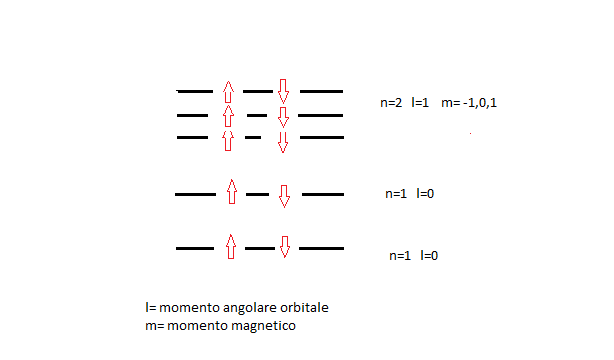
\includegraphics[scale=1]{immagini/occupazione-livelli.png}
\end{center}
Arriva un momento in cui tutti i livelli sono occupati:\\
\begin{equation}
\int_{0}^{E}D(E)E\,dE=N
\end{equation}
dove D(E) è la densità di energia.\\
Trovo:
\begin{equation}
E_{F}=\dfrac{\hbar^{2}}{2m}(\dfrac{3\pi^2N}{V})^{2/3}
\end{equation}
è un energia molto alta.
 \begin{equation}
T_{B}k_{B}=E_{B}  \textrm{  bose} 
\end{equation}

\subsection{Andamento Potenziale Chimico $\mu$}
Fermi:\\
All' inizio posso prendere $\mu=E_{F}$
\begin{center}
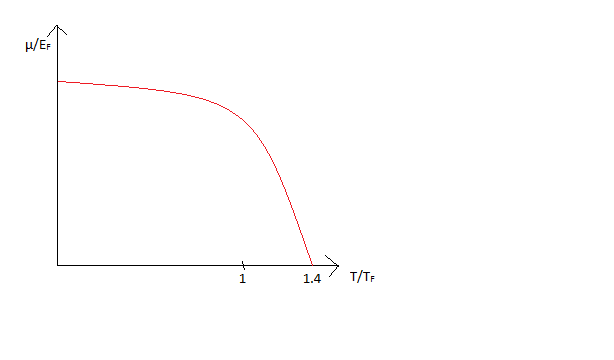
\includegraphics[scale=1]{immagini/pot-chimico-fermi.png} 
\end{center}
Bose:\\
All' inizio posso prendere $\mu=0$
\begin{center}
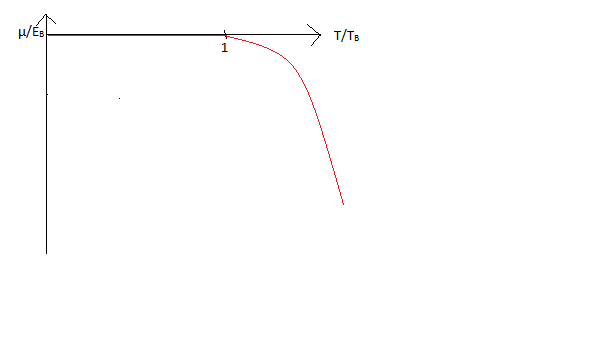
\includegraphics[scale=1]{immagini/pot-chimico-bose.png}
\end{center}

\subsection{Numero di occupazione medio ( in funzione dell'energia)}
Fermi: \\ Tutti gli elettroni cercano di occupare lo stato fondamentale.
Alzando la temperatura si svuotano i livelli sotto $E_{F}$ e si riempono quelli sopra.
\begin{center}
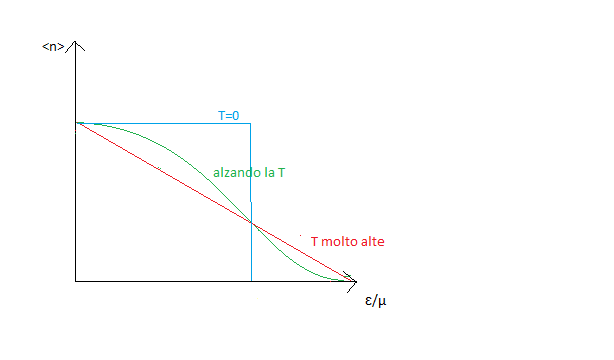
\includegraphics[scale=1]{immagini/n-occ-fermi.png}
\end{center}
Bose:\\ Aumentando T si svuota lo stato fondamentale e si riempono gli stati sopra.
Per T molto grande si ha uno svuotamento netto. Per T piccolo ho un addensamento a energia minima.
\begin{center}
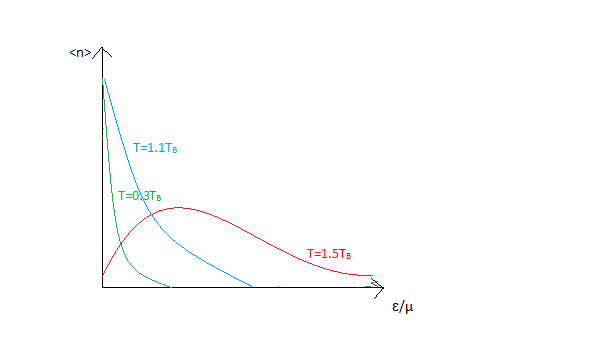
\includegraphics[scale=1]{immagini/n-occ-bose.png}
\end{center}
 
\subsection{Energia Bose}
La curva tende asintoticamente alla retta di Dulong-Petit.
\begin{center}
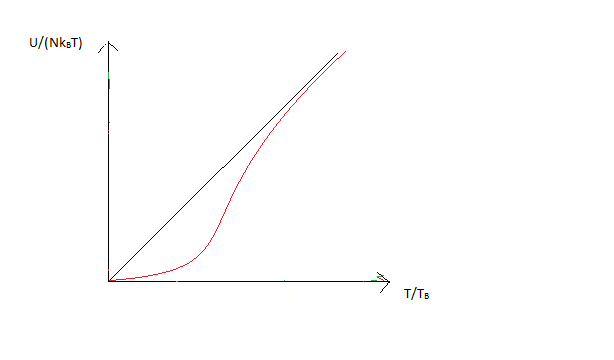
\includegraphics[scale=1]{immagini/energia-bose.png}
\end{center}

\subsection{Calore specifico Bose}
\begin{center}
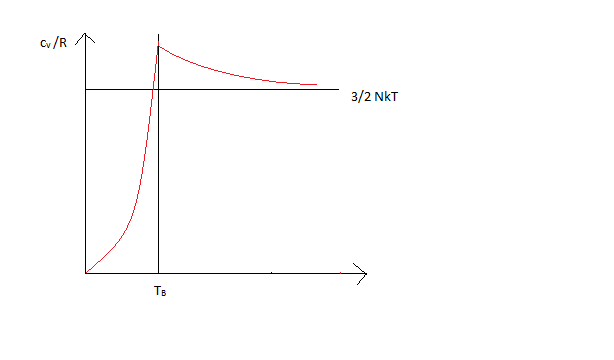
\includegraphics[scale=1]{immagini/calore-spec-bose.png}
\end{center}
Dove $c_{v}$ è il calore specifico e R è la costante dei gas. Da questo grafico si vede bene la transizione di fase. 
$N_{0}/N$ BOSE:
\begin{center}
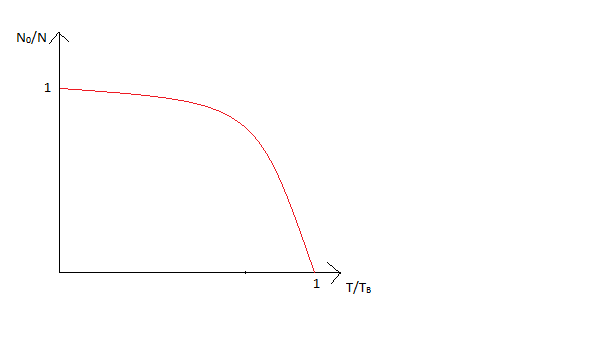
\includegraphics[scale=1]{immagini/ultimo-graf-bose.png}
\end{center}
Ho trovato che la termodinamica dei gas perfetti quantistici è determinato da 2 oggetti: il numero di occupazione medio del livello di energia e la densità di stati.
%\end{document} %TRASCRITTO*
%11 Non località quantistica - Disuguaglianza di Bell
\chapter[Non località quantistica]{Non località quantistica - Disuguaglianza di Bell} %Non località quantistica - Disuguaglianza di Bell
\section{Macchinette di Popescu} %Macchinette di Popescu
Ci sono Alice $A$ e Bob $B$, fidanzati, che devono separarsi. Lei rimane sulla Terra e lui va in un pianeta lontanissimo. Vogliono comunicare simultaneamente e si rivolgono a Popescu. Egli fornisce loro due macchinette che comunicano in binario:
\begin{itemize}
\item Alice: pulsante $x=0,1$ lampadina $a=0,1$
\item Bob: pulsante $y=0,1$ lampadina $b=0,1$
\end{itemize}

Tornando a casa le provano. Le variabili $x$ e $y$ però non sono variabili e rimangono fisse su $0$. In compenso $a$ e $b$ funzionano perfettamente: \\
\begin{tabularx}{\textwidth}{XXXXX}
\toprule
$x$ & $y$ & $a$ & $b$ & $P\left(a,b|x,y\right)$ \\
\midrule
$0$ & $0$ & $0$ & $0$ & $\frac{1}{2}$ \\
$0$ & $0$ & $1$ & $1$ & $\frac{1}{2}$ \\
\bottomrule
\end{tabularx}
Si nota che si potrebbe costruire entrambe le macchinette con una memoria interna condivisa:
Mem$_a=011001110110001$ Mem$_b=011001110110001$.

Tornando da Popescu, egli da loro due macchinette con i pulsanti funzionanti: \\
\begin{tabularx}{\textwidth}{XXXXX}
\toprule
$x$ & $y$ & $a$ & $b$ & $P\left(a,b|x,y\right)$ \\
\midrule
$0$ & $0$ & $0$ & $0$ & $\frac{1}{2}$ \\
$0$ & $0$ & $1$ & $1$ & $\frac{1}{2}$ \\
$1$ & $0$ & $0$ & $1$ & $\frac{1}{2}$ \\
$1$ & $0$ & $1$ & $0$ & $\frac{1}{2}$ \\
$0$ & $1$ & $0$ & $1$ & $\frac{1}{2}$ \\
$0$ & $1$ & $1$ & $0$ & $\frac{1}{2}$ \\
$1$ & $1$ & $0$ & $0$ & $\frac{1}{2}$ \\
$1$ & $1$ & $1$ & $1$ & $\frac{1}{2}$ \\
\bottomrule
\end{tabularx}
Si nota la presenza ancora di memorie interne condivise.

Tornando ancora da Popescu, egli da una versione migliorata delle macchinette: \\
\begin{tabularx}{\textwidth}{XXXXX}
\toprule
$x$ & $y$ & $a$ & $b$ & $P\left(a,b|x,y\right)$ \\
\midrule
$0$ & $0$ & $0$ & $0$ & $\frac{1}{2}$ \\
$0$ & $0$ & $1$ & $1$ & $\frac{1}{2}$ \\
$1$ & $0$ & $0$ & $0$ & $\frac{1}{2}$ \\
$1$ & $0$ & $1$ & $1$ & $\frac{1}{2}$ \\
$0$ & $1$ & $0$ & $0$ & $\frac{1}{2}$ \\
$0$ & $1$ & $1$ & $1$ & $\frac{1}{2}$ \\
$1$ & $1$ & $0$ & $1$ & $\frac{1}{2}$ \\
$1$ & $1$ & $1$ & $0$ & $\frac{1}{2}$ \\
\bottomrule
\end{tabularx}
Questa volta non si nota la memoria condivisa, ma non sono ancora perfette.

Vanno per l'ultima volta da Popescu: \\
\begin{tabularx}{\textwidth}{XXXXX}
\toprule
$x$ & $y$ & $a$ & $b$ & $P\left(a,b|x,y\right)$ \\
\midrule
$0$ & $0$ & $0$ & $0$ & $\frac{3}{4}$ \\
$0$ & $0$ & $1$ & $1$ & $\frac{1}{4}$ \\
$1$ & $0$ & $0$ & $1$ & $\frac{3}{4}$ \\
$1$ & $0$ & $1$ & $0$ & $\frac{1}{4}$ \\
$0$ & $1$ & $0$ & $1$ & $\frac{1}{4}$ \\
$0$ & $1$ & $1$ & $0$ & $\frac{3}{4}$ \\
$1$ & $1$ & $0$ & $0$ & $\frac{1}{4}$ \\
$1$ & $1$ & $1$ & $1$ & $\frac{3}{4}$ \\
\bottomrule
\end{tabularx}
Con questa finalmente si ha comunicazione.

%MANCA UNA PARTE

Tornano da Popescu e chiedono come funzioni l'ultima macchinetta. Egli non rivela come costruirla ma permette di conoscere il metodo per la terza. Il metodo è molto simile alla meccanica quantistica...

Pensando al singoletto $\frac{i}{\sqrt{2}}\left |\sigma_y \right\rangle\rangle=\frac{i}{\sqrt{2}}\left(\left |-1 \right\rangle\otimes\left |1 \right\rangle-\left |1 \right\rangle\otimes\left |-1 \right\rangle\right)$ si ha:
\begin{equation}\begin{split}
U\otimes U^{\dag}\frac{i}{\sqrt{2}}\left |\sigma_y \right\rangle\rangle=\\
=\frac{i}{\sqrt{2}}\left.\left |U\sigma_y U^{\dag}\sigma_y\sigma_y \right\rangle\right\rangle=\\
=\frac{i}{\sqrt{2}}\left.\left |UU^{\dag}\sigma_y \right\rangle\right\rangle=\\
=\frac{i}{\sqrt{2}}\left |\sigma_y \right\rangle\rangle
\end{split}\end{equation}
e si nota che esso è invariante per rotazioni.

%MANCA UNA PARTE

Questa si può descrivere con variabili condivise. Ci si trova nella strssa condizione della seconda tabella.

C'è però un caso che non rientra in quelli precedenti: la misura viene fatta a 45º.

\section{Disuguaglianza di CHSH (Clauser, Horn, Shimmony, Holt)} %Disuguaglianza di CHSH (Clauser, Horn, Shimmony, Holt)
Si hanno variabili random per Alice $\sigma_z=z_A$, $\sigma_x=x_A$ e per Bob $\frac{1}{\sqrt{2}}\left(\sigma_x+\sigma_z\right)=w_B$, $\frac{1}{\sqrt{2}}\left(\sigma_x-\sigma_z\right)u_B$.
\begin{equation}\begin{split}
z_Aw_B+x_Aw_B+x_Au_B-z_Au_B=\left(z_A+x_A\right)w_B+\left(x_A-z_A\right)u_B= \pm 2
\end{split}\end{equation}
Si ricava il bound CHSH:
\begin{equation}\begin{split}
\left | \mathbb{E}\left[\left(z_A+x_A\right)w_B+\left(x_A-z_A\right)u_B\right] \right |\le 2
\end{split}\end{equation}

\subsection{Disuguaglianza nella meccanica quantistica} %Disuguaglianza nella meccanica quantistica
Nella meccanica quantistica si hanno le aspettazioni:
\begin{equation}\begin{split}
\mathbb{E}\left(z_A,w_B\right)=\\
=\frac{1}{2}\left\langle\langle \sigma_y\right |\sigma_z\otimes\frac{1}{\sqrt{2}}\left(\sigma_x+\sigma_z\right)\left |\sigma_y \right\rangle\rangle=\\
\frac{1}{2\sqrt{2}}\left\langle\left\langle \sigma_y|\sigma_z\sigma_y\left(\sigma_x+\sigma_z\right) \right\rangle\right\rangle=\\
\frac{1}{2\sqrt{2}}Tr\left[\sigma_y\sigma_z\sigma_y\sigma_z\right]=\\
=-\frac{1}{\sqrt{2}}
\end{split}\end{equation}
\begin{equation}\begin{split}
\mathbb{E}\left(z_A,u_B\right)=\frac{1}{\sqrt{2}}
\end{split}\end{equation}
\begin{equation}\begin{split}
\mathbb{E}\left(x_A,w_B\right)=\\
=\frac{1}{2}\left\langle\left\langle \sigma_y|\sigma_x\otimes\frac{1}{\sqrt{2}}\left(\sigma_x+\sigma_z\right)\sigma_y \right\rangle\right\rangle=\\
=\frac{1}{2\sqrt{2}}Tr\left[\sigma_y\sigma_x\sigma_y\sigma_x\right]=\\
=-\frac{1}{\sqrt{2}}
\end{split}\end{equation}
\begin{equation}\begin{split}
\mathbb{E}\left(x_A,u_B\right)=\\
=\frac{1}{2}\left\langle\left\langle \sigma_y|\sigma_x\otimes\frac{1}{\sqrt{2}}\left(\sigma_x-\sigma_z\right)\sigma_y \right\rangle\right\rangle=\\
=\frac{1}{2\sqrt{2}}Tr\left[\sigma_y\sigma_x\sigma_y\sigma_x\right]=\\
=-\frac{1}{\sqrt{2}}
\end{split}\end{equation}
usando le regole $\left.\left\langle A|B \right\rangle\right\rangle=Tr\left[A^{\dag}B\right]$ e $\left(A\otimes B\right)\left.\left |C \right\rangle\right\rangle=\left.\left |ACB^{t} \right\rangle\right\rangle$

Si ricava infine
\begin{equation}\begin{split}
\mathbb{E}\left(z_Aw_B+x_Aw_B+x_Au_B-z_Au_B\right)=-\frac{1}{\sqrt{2}}-\frac{1}{\sqrt{2}}-\frac{1}{\sqrt{2}}-\frac{1}{\sqrt{2}}=-2\sqrt{2}
\end{split}\end{equation}
che víola il bound di CHSH (si ricordi che il bound prevede che venga considerato il modulo dell'aspettazione). Questo dimostra che la visione realista della meccanica quantistica è totalmente sbagliata.

\section{Correlazioni EPR (Einstein, Podoloski, Rosen)} %Correlazioni EPR (Einstein, Podoloski, Rosen)

%MANCA TUTTO

\section{Caso GHZ (Greenberger, Horn, Zeilinger)} %Caso GHZ (Greenberger, Horn, Zeilinger)
Sia $\left |\psi  \right\rangle=\frac{1}{\sqrt{2}}\left(\left |000 \right\rangle-\left |111 \right\rangle\right)$.
\begin{equation}\begin{split}
\sigma_{1x}\sigma_{2y}\sigma_{3y}\left |\psi  \right\rangle=\left |\psi  \right\rangle \\
\sigma_{1y}\sigma_{2x}\sigma_{3y}\left |\psi  \right\rangle=\left |\psi  \right\rangle \\
\sigma_{1y}\sigma_{2y}\sigma_{3x}\left |\psi  \right\rangle=\left |\psi  \right\rangle \\
\sigma_{1x}\sigma_{2x}\sigma_{3x}\left |\psi  \right\rangle=-\left |\psi  \right\rangle
\end{split}\end{equation}

\begin{equation}\begin{split}
m_{1x}m_{2y}m_{3y}=+1 \\
m_{1y}m_{2x}m_{3y}=+1 \\
m_{1y}m_{2y}m_{3x}=-1 \\
m_{1x}m_{2x}m_{3x}=+1
\end{split}\end{equation}
Si ha quindi una contraddizione.

\section{Variabili locali non osservabili} %Variabili locali non osservabili
Si prenda $\left\{\left |n \right\rangle\right\}$:
\begin{equation}\begin{split}
\sum{\left |n \right\rangle\left\langle n\right |a_n}=A
\end{split}\end{equation}
Si prende un'osservabile e si fa:
\begin{equation}\begin{split}
\frac{1}{2}\left.\left |\sigma_{x} \right\rangle\right\rangle\left\langle\left\langle \sigma_{x} \right.\right |+\\
\frac{1}{2}\left.\left |\sigma_{y} \right\rangle\right\rangle\left\langle\left\langle \sigma_{y} \right.\right |+\\
\frac{1}{2}\left.\left |\sigma_{z} \right\rangle\right\rangle\left\langle\left\langle \sigma_{z} \right.\right |+\\
\frac{1}{2}\left.\left |\mathbb{I}\right\rangle\right\rangle\left\langle\left\langle \mathbb{I} \right.\right |=\\
\mathbb{I}\otimes\mathbb{I}
\end{split}\end{equation}

\begin{equation}\begin{split}
\left[\frac{1}{2}\left.\left |\sigma_{\alpha} \right\rangle\right\rangle\left\langle\left\langle \sigma_{\alpha } \right.\right |, \bar \sigma\cdot \bar n\otimes\mathbb{I}\right]\neq 0 \quad \forall \bar n
\end{split}\end{equation} 
\section{Esperimento di Stern e Gerlach} %Esperimento di Stern e Gerlach
Considero un sistema di particelle con momento angolare di spin 1/2, in moto lungo y, soggette ad un campo magnetico con un gradiente lungo la direzione z.
\begin{center}
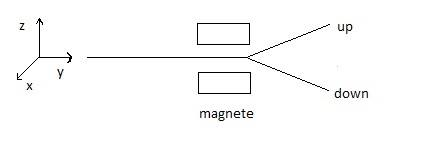
\includegraphics[scale=0.5]{immagini/stern-gerlach.jpg} %immagine
\end{center}

Il gradiente produce una forza traslazionale che direziona le particelle verso l'alto o verso il basso, a seconda che lo spin sia rispettivamente up o down. \\
I due autovalori dell'energia corrispondenti ai due gradi di libertà di spin, sono
\begin{equation}\begin{split}
E_{\pm}=\pm\gamma(B_{0}+\alpha z)\frac{\hbar}{2}
\end{split}\end{equation}
con $\gamma>0$ rapporto giromagnetico  e  $\alpha$ gradiente lungo z.\\
Prese le particelle in un particolare stato iniziale, le collimiamo selezionando quelle con un valore preciso della velocità; queste particelle le preparo poi in uno stato di sovrapposizione di spin up e spin down:
\begin{equation}\begin{split}
c_{\uparrow}\left|\uparrow\right\rangle+c_{\downarrow}\left|\downarrow\right\rangle
\end{split}\end{equation}
dove, per la condizione di normalizzazione risulta
\begin{equation}\begin{split}
\left|c_{\uparrow}\right|^2 = p
\end{split}\end{equation}
\begin{equation}\begin{split}
\left|c_{\downarrow}\right|^2 = 1-p
\end{split}\end{equation}
Il sistema considerato presenta due gradi di libertà per particella: la coordinata x (dipendente dal tempo) che però non è rilevante ai fini della nostra indagine perché abbiamo preparato le particelle in modo che traslino con velocità costante; e il tempo di nostro interesse.\\
Dopo un tempo di volo T, le particelle si raggruppano in due macchie distinte e simmetriche rispetto alla direzione di volo.\\
Consideriamo una particella nello stato iniziale
\begin{equation}\begin{split}
\left|z_{0}\right\rangle (c_{\uparrow}\left|\uparrow\right\rangle+c_{\downarrow}\left|\downarrow\right\rangle)
\end{split}\end{equation}
applichiamo l'Hamiltoniana (che supponiamo agire per un dato periodo) e ne facciamo la rappresentazione z\\
\begin{equation}\begin{split}
\left\langle z\right| \exp (-\frac{itH}{\bar{h}})\left|z_{0}\right\rangle (c_{\uparrow}\left|\uparrow\right\rangle+c_{\downarrow}\left|\downarrow\right\rangle)=\\
\textrm{sostituendo gli autovalori}\\
=c_{\uparrow}\exp(i \gamma T B_{0}\frac{1}{2}) \left|\uparrow\right\rangle \exp(i \alpha \gamma \frac{T}{2}z)+ c_{\downarrow}\exp(-i \gamma T B_{0}\frac{1}{2}) \left|\downarrow\right\rangle \exp(-i \alpha \gamma \frac{T}{2}z)=\\
=c_{\uparrow}\left|\uparrow\right\rangle \left|1\right\rangle_{ORB} + c_{\downarrow}\left|\downarrow\right\rangle \left|2\right\rangle_{ORB}
\end{split}\end{equation}
dove $\left|\uparrow\right\rangle$ e $\left|\downarrow\right\rangle$ rappresentano lo stato di spin e $\left|1\right\rangle$ e $\left|2\right\rangle$ lo stato orbitale.\\
Da questa descrizione si sa che:
\begin{itemize}
\item se preparo una particella in uno stato up $\left|\uparrow\right\rangle$ (ponendo $c_{\uparrow}=1$ e $c_{\downarrow}=0$)\\la ritrovo nello stato up $\left|\uparrow\right\rangle \left|1\right\rangle_{ORB}$;
\item se preparo una particella in uno stato down $\left|\downarrow\right\rangle$ (ponendo $c_{\uparrow}=0$ e $c_{\downarrow}=1$)\\la ritrovo nello stato down $\left|\downarrow\right\rangle \left|2\right\rangle_{ORB}$;
\item se invece preparo le particelle in una sovrapposizione ottengo uno stato entangled.
\end{itemize}
\subsection{Interpretazione}
Il termine $\left|c_{\uparrow}\right|^2$ rappresenta la probabilità di trovare la particella nello stato up
il termine $\left|c_{\downarrow}\right|^2$ rappresenta la probabilità di trovare la particella nello stato down. Se preparo le particelle in una sovrapposizione, esse saranno in due differenti autostati della posizione, non sono in una mistura tra stato up e stato down ma in uno stato entangled.

\section{Gatto di Schrödinger} %Gatto di Schrödinger
Schrödinger propose un paradosso con il quale riuscì a enfatizzare il problema concettuale emerso nell'esperimento di Stern e Gerlach:

Un gatto viene messo in una stanza con pareti metalliche insieme con il seguente congegno infernale [...] All'interno di un contatore Geiger c'è una piccolissima quantità di sostanza radioattiva, così piccola che c'è un'uguale probabilità che in un'ora decada uno degli atomi o che non ne decada nessuno. Se uno decade, allora il contatore scatta e tramite un relè attiva un martelletto che rompe una fiala contenente cianuro. Se si prepara tutto il sistema e si aspetta un'ora, si può dire che il gatto è vivo se non è decaduto nessun atomo ed è morto se è decaduto anche solo un atomo.

La sostanza radioattiva si trova in uno stato di sovrapposizione: decaduta - non decaduta.
\begin{itemize}
\item Se la sostanza non decade il gatto è vivo cioè siamo in uno stato $\left|\psi_{vivo}\right\rangle$;
\item Se la sostanza decade il gatto è morto cioè siamo in uno stato $\left|\psi_{morto}\right\rangle$;
\item Se faccio una sovrapposizione (partendo con il gatto vivo)
\begin{equation}\begin{split}\begin{split}
(c_{\uparrow}\left|\uparrow\right\rangle + c_{\downarrow}\left|\downarrow\right\rangle)\left|\psi_{vivo}\right\rangle=\\
=c_{\uparrow}\left|\uparrow\right\rangle\left|\psi_{vivo}\right\rangle + c_{\downarrow}\left|\downarrow\right\rangle\left|\psi_{morto}\right\rangle
\end{split}\end{split}\end{equation}
ottengo uno stato entangled nel quale il gatto non è né vivo né morto.
\end{itemize}

Si crea un problema concettuale: se vedo la particella in un posto ben preciso, essa dovrebbe essere in un autostato della posizione ben preciso (cioè il gatto dove essere vivo o morto) non può essere entangled.

\section{Von Neumann} %Von Neumann
Von Neumann interviene in questa descrizione affermando che nella misura interferisce anche la nostra mente: quando io guardo il gatto la mia mente risulta in uno stato entangled con la convinzione che il gatto sia vivo quando la particella non è decaduta, e con la convinzione che il gatto sia morto quando la particella è decaduta.\\
Von Neumann sostiene che in questa catena ci debba essere qualcosa, alla fine, che deve collassare; questo è necessario affinché sia verificato il postulato di Von Neumann, cioè se il risultato è su si deve trovare nell'autostato su, mentre se il risultato è giu si deve trovare nell'autostato giù.\\
Questo collasso viene nel cervello, cioè lo creo io quando decido il risultato, che è un dato obiettivo e quindi associato ad uno stato preciso.
Il problema è che se collassa un elemento della catena collassa tutto.

Consideriamo lo stato
\begin{equation}\begin{split}
\frac{1}{2}(\left|\uparrow\right\rangle \left|1\right\rangle + \left|\downarrow\right\rangle \left|2\right\rangle)(\left\langle \uparrow\right| \left\langle 1\right| + \left\langle \downarrow\right|\left\langle 2\right|)
\end{split}\end{equation} 
e applichiamo Von Neumann, cioè prendiamo un qualunque stato $\rho$ e lo proiettiamo:
\begin{equation}\begin{split}
\left|1\right\rangle \left\langle 1\right| \rho \left|1\right\rangle \left\langle 1\right|=\left|1\right\rangle \left\langle 1\right| p_{1}=\left\langle 1\right| p_{1} \left|1\right\rangle
\end{split}\end{equation}
(dove $p_{1}$ rappresenta la probabilità data dalla regola di Bohr) otteniamo quindi:
\begin{equation}\begin{split}
\frac{1}{2} \left|\uparrow\right\rangle \left\langle\uparrow\right| \left|1\right\rangle \left\langle 1\right| + \frac{1}{2}\left|\downarrow\right\rangle \left\langle\downarrow\right| \left|2\right\rangle \left\langle 2\right|\rangle\
\end{split}\end{equation}
che rappresenta non uno stato entanglement ma una mistura.

Definisco gli \textbf{stati bipartiti}:
\begin{equation}\begin{split}
\left|\psi_{1}\right\rangle=\left|\uparrow\right\rangle \left|1\right\rangle
\end{split}\end{equation}
\begin{equation}\begin{split}
\left|\psi_{2}\right\rangle=\left|\downarrow\right\rangle \left|2\right\rangle
\end{split}\end{equation}
lo stato entangled $c_{\uparrow}\left|\psi_{1}\right\rangle + c_{\downarrow}\left|\psi_{2}\right\rangle$ ha una matrice densità del tipo:\\
\begin{equation}\begin{split}
\rho=
\left(\begin{matrix}
\left|c_{\uparrow}\right|^2\quad c_{\uparrow}c_{\downarrow}^* \\
c_{\uparrow}^*c_{\downarrow} \quad \left|c_{\downarrow}\right|^2
\end{matrix}\right)
\end{split}\end{equation}
mentre secondo Von Neumann rimane solo la mistura cioè una matrice del tipo:
\begin{equation}\begin{split}
\rho=
\left(\begin{matrix}
\left|c_{\uparrow}\right|^2\quad 0 \\
0 \quad \left|c_{\downarrow}\right|^2
\end{matrix}\right)
\end{split}\end{equation}
che corrisponde a dire che ho solo due possibilità: la particella si trova su o giù con una data probabilità, il gatto è vivo o morto.\\
E' possibile indipendentemente da Von Neumann, calcolare lo stato, analizzando l'interazione con la meccanica quantistica (l'unico problema rimane il collasso del pointer).

Consideriamo un sistema di questo tipo:
\begin{center}
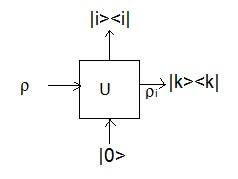
\includegraphics[scale=0.5]{immagini/von-neumann.jpg} %immagine
\end{center}
Prendiamo uno stato misto generico iniziale $\rho$ che interagisce mediante una trasformazione unitaria con un sistema ancillare, che prepariamo in un sistema di riferimento zero e che gioca il ruolo di pointer.\\
Nell'esperimento di Stern e Gerlach il sistema rappresenta lo spin e l'ancilla è il grado orbitale; mentre nel paradosso di Schrödinger il sistema è la particella che decade e l'ancilla è il gatto.\\
Si misura poi un'osservabile i che è associata ad un set ortonormale $\{\left|i\right\rangle\}$ tale che $I=\sum_{i}\left|i\right\rangle\left\langle i\right|$.
All'uscita il sistema entra in un nuovo apparato di misura dove facciamo un'altra misura sul sistema chiamata $\left|k\right\rangle\left\langle k\right|$, associata ad un altro set ortonormale $\{\left|k\right\rangle\}$ tale che $I=\sum_{k}\left|k\right\rangle\left\langle k\right|$.
Calcoliamo la probabilità congiunta di vedere il risultato $i$ sull'ancilla e il risultato $k$ nella misura fatta sul sistema:
\begin{equation}\begin{split}
p(i,k)=tr[\left|k\right\rangle\left\langle k \right|\otimes\left|i\right\rangle\left\langle i \right| U (\rho\otimes \left|0\right\rangle\left\langle 0\right|)U^+]
\end{split}\end{equation}
(utilizzando la regola di Born e la Schrödinger picture). \\
Si calcola poi la probabilità marginale di vedere i indipendentemente da ciò che si vede dopo:
\begin{equation}\begin{split}
p(i)=\sum_{k}p(1,k)=tr[I\otimes \left|i\right\rangle \left\langle i\right| U (\rho\otimes \left|0\right\rangle\left\langle 0\right|) U^+]
\end{split}\end{equation}
Calcoliamo la probabilità condizionata di vedere k se abbiamo visto i (con la formula di Bayes):
\begin{equation}\begin{split}
p(k|i)=\frac{p(i,k)}{p(i)}
\end{split}\end{equation}
All'uscita della prima misura il sistema si trova in uno stato $\rho_{i}$ tale che:
\begin{equation}\begin{split}
tr[\rho_{i}\left|k\right\rangle\left\langle k\right|]=p(k|i)
\end{split}\end{equation}
ricavo $\rho_{i}$:
\begin{equation}\begin{split}
p(k|i)=\frac{p(i,k)}{p(i)}=\\
\frac{tr[\left|k\right\rangle\left\langle k\right| tr_{2}[(I\otimes\left|i\right\rangle\left\langle i\right|)U(\rho\otimes\left|0\right\rangle\left\langle 0\right|)U^+]]}{tr[(I\otimes\left|i\right\rangle\left\langle i\right|) U (\rho\otimes\left|0\right\rangle\left\langle 0\right|)U^+]}
\end{split}\end{equation}
sappiamo che la traccia parziale di un operatore (R) si calcola come somma su\\un set ortonormale di:
\begin{equation}\begin{split}
tr_{2}[R]= \sum_{i}(I\otimes\left\langle i\right|)R(I\otimes\left|i\right\rangle)
\end{split}\end{equation}
utilizzando l'invarianza della traccia per permutazione ciclica e le decomposizioni $I\otimes\left|i\right\rangle\left\langle i\right|=(I\otimes\left|i\right\rangle)(I\otimes\left\langle i\right|)$  $\rho\otimes\left|0\right\rangle\left\langle 0\right|=(\rho\otimes I)(I\otimes\left|0\right\rangle)(I\otimes\left\langle0\right|)$ otteniamo:
\begin{equation}\begin{split}
tr_{2}[(I\otimes\left|i\right\rangle\left\langle i\right|)U(\rho\otimes\left|0\right\rangle\left\langle 0\right|)U^+]=\\
=(I\otimes\left\langle i\right|)U(I\otimes\left|0\right\rangle)\rho(I\otimes\left\langle 0\right|)U^+(I\otimes\left|i\right\rangle)= \\
=A_{i}\rho A_{i}^+
\end{split}\end{equation}
con $A_{i}=(I\otimes\left\langle i\right|)U(I\otimes\left|0\right\rangle)$ dove:
$(I\otimes\left\langle i\right|)$ rappresenta l'osservabile che misuriamo sul pointer, $U$ l'interazione unitaria tra sistema e ancilla, $(I\otimes\left|0\right\rangle)$ la preparazione del pointer/dell'ancilla cioè lo $z_{0}$ delle particelle. \\
Si ricava quindi:
\begin{equation}\begin{split}
\rho_{i}=\frac{A_{i}\rho A_{i}^+}{tr[A_{i}\rho A_{i}^+]}
\end{split}\end{equation}
che rappresenta lo stato che esce dall'apparato di misura dopo che ho letto il risultato, uno stato condizionato dalla conoscenza del risultato della misura precedente. \\
Abbiamo ottenuto questa relazione solamente utilizzando la regola di Born e rompendo lo stato entangled con Von Neumann.\\
Alla fine dell'interazione tra stato e misura, lo stato non è entangled ma resta solo una mistura tra gli stati che corrispondono ai due possibili risultati (stati che so calcolare). %TRASCRITTO*

\part{APPLICAZIONI}
\chapter{Perturbazioni stazionarie} %Perturbazioni stazionarie %MANCA
\input{capitoli2/11-12-2013} %MANCA
\input{capitoli2/11-13-2013} %MANCA
\section{Livello doppiamente degenere} %Livello doppiamente degenere
\begin{equation}\begin{split}
\begin{cases}
H_0\left |\psi _a^{\left(0\right)} \right\rangle=E^{\left(0\right)}\left |\psi _a^{\left(0\right)} \right\rangle \\
H_0\left |\psi _b^{\left(0\right)} \right\rangle=E^{\left(0\right)}\left |\psi _b^{\left(0\right)} \right\rangle
\end{cases}
\end{split}\end{equation}
Si ha:
\begin{equation}\begin{split}
H_0\left(\alpha\left |\psi _a ^{\left(0\right)}\right\rangle+\beta\left |\psi _b^{\left(0\right)} \right\rangle\right)=E^{\left(0\right)}\left(\alpha\left |\psi _a ^{\left(0\right)}\right\rangle\beta\left |\psi _b^{\left(0\right)} \right\rangle\right)
\end{split}\end{equation}

Sia:
\begin{equation}\begin{split}
H=H_0+H_P=H_0+\lambda H_0
\end{split}\end{equation}
\begin{equation}\begin{split}
H\left |\psi  \right\rangle=E\left |\psi  \right\rangle
\end{split}\end{equation}
\begin{equation}\begin{split}
\begin{cases}
E=E^{\left(0\right)}+\lambda E^{\left(1\right)}=E^{\left(0\right)}+\delta E^{\left(1\right)} \\
\left |\psi  \right\rangle=\left |\psi ^{\left(0\right)} \right\rangle+\lambda\left |\psi ^{\left(1\right)} \right\rangle=\left |\psi ^{\left(0\right)} \right\rangle+\left |\delta\psi ^{\left(1\right)} \right\rangle
\end{cases}
\end{split}\end{equation}

Si ricava $\lambda$:
\begin{equation}\begin{split}
H_0\left |\psi ^{\left(1\right)} \right\rangle+H'\left |\psi ^{\left(0\right)} \right\rangle=E^{\left(0\right)}\left |\psi ^{\left(1\right)} \right\rangle+E^{\left(1\right)}\left |\psi ^{\left(0\right)} \right\rangle \\
\left\langle \psi _a^{\left(0\right)}|H_0|\psi ^{\left(1\right)} \right\rangle+\left\langle \psi _a^{\left(0\right)}|H'|\psi ^{\left(0\right)} \right\rangle=E^{\left(0\right)}\left\langle \psi _a^{\left(0\right)}|\psi ^{\left(1\right)} \right\rangle+E^{\left(1\right)}\left\langle \psi _a^{\left(0\right)}|\psi ^{\left(0\right)} \right\rangle
\end{split}\end{equation}
\begin{equation}\begin{split}
\begin{cases}
\alpha\left\langle \psi _a^{\left(0\right)}|H'|\psi _a^{\left(0\right)} \right\rangle+\beta\left\langle \psi _a^{\left(0\right)}|H'|\psi _b^{\left(0\right)} \right\rangle=E^{\left(1\right)}\alpha \\
\alpha\left\langle \psi _b^{\left(0\right)}|H'|\psi _a^{\left(0\right)} \right\rangle+\beta\left\langle \psi _b^{\left(0\right)}|H'|\psi _b^{\left(0\right)} \right\rangle=E^{\left(1\right)}\beta
\end{cases}
\end{split}\end{equation}

%MANCA UNA PARTE

\section{Correzione agli autovalori} %Correzione agli autovalori
\begin{equation}\begin{split}
\left(H_0-E^{\left(0\right)}\right)\left |\psi _i^{\left(1\right)} \right\rangle=-\left(H'-E_i^{\left(1\right)}\right)\left |\psi _i^{\left(0\right)} \right\rangle
\end{split}\end{equation}
Si supponga di avere $\psi _i$:
\begin{equation}\begin{split}
\left |\psi _i^m \right\rangle+\sum_{m \textrm{ degenere}}{\gamma_m\left |\psi _m^{\left(0\right)} \right\rangle}
\end{split}\end{equation}

%MANCA UNA PARTE

\begin{equation}\begin{split}
\left(H_0-E^{\left(0\right)}\right)\sum_{m\textrm{ deg}}{c_m^{\left(i\right)}\left |\psi _m^{\left(0\right)} \right\rangle}=\\
=-\left(H'-E^{\left(1\right)}\right)\left |\psi _i^{\left(0\right)} \right\rangle=\\
=\sum_{m\textrm{ deg}}{c_m^{\left(i\right)}\left(E_m^{\left(0\right)}-E^{\left(0\right)}\right)}\left |\psi _m^{\left(0\right)} \right\rangle
\end{split}\end{equation}
Con $n$ dentro al sottospazio degenere
\begin{equation}\begin{split}
\sum_{m\textrm{ deg}}{c_m^{\left(i\right)}\left(E_m^{\left(0\right)}-E^{\left(0\right)}\right)}\left\langle \psi _n^{\left(0\right)}|\psi _m^{\left(0\right)} \right\rangle=\\
=-\left\langle \psi _n^{\left(0\right)}|H'-E_i^{\left(1\right)}|\psi _i^{\left(0\right)} \right\rangle=\\
=\left\langle \psi _n^{\left(0\right)}|H'|\psi _i^{\left(0\right)} \right\rangle+E_i^{\left(0\right)}\left\langle \psi _i^{\left(0\right)}|\psi _i^{\left(0\right)} \right\rangle
\end{split}\end{equation}
Con $n$ dentro al sottospazio degenere
\begin{equation}\begin{split}
c_n^{\left(i\right)}\left(E_n^{\left(0\right)}-E^{\left(0\right)}\right)=-\left\langle \psi _0^{\left(0\right)}|H'|\psi _i^{\left(0\right)} \right\rangle \\
\Longrightarrow c_n^{\left(i\right)}=\frac{\left\langle \psi _0^{\left(0\right)}|H'|\psi _i^{\left(0\right)} \right\rangle}{\left(E^{\left(0\right)}-E_n^{\left(0\right)}\right)}
\end{split}\end{equation}

In definitiva:
\begin{equation}\begin{split}
\left |\psi _i^{\left(1\right)} \right\rangle=\sum_{m\textrm{ deg}}{\frac{\left\langle \psi _0^{\left(0\right)}|H'|\psi _i^{\left(0\right)} \right\rangle}{\left(E^{\left(0\right)}-E_m^{\left(0\right)}\right)}\left |\psi _m^{\left(0\right)} \right\rangle}
\end{split}\end{equation}

%MANCA UNA PARTE

\begin{teorema}
Sia $A$ e che esso commuti con $H'$:
\begin{equation}\begin{split}
\left[A,H_0\right]=\left[A,H'\right]=0.
\end{split}\end{equation}
%MANCA U A PARTE
\end{teorema}
\begin{proof}
\begin{equation}\begin{split}
\left\langle \psi _a|\left[A,H'\right]|\psi _b \right\rangle=0 \\
=\left\langle \psi _a|AH'|\psi _b \right\rangle-\left\langle \psi _a|H'A|\psi _b \right\rangle=
=\mu\left\langle \psi _a|H'|\psi _b \right\rangle-\nu\left\langle \psi _a|H'|\psi _b \right\rangle=H'_{a,b}\left(\mu-\nu\right)=0
\end{split}\end{equation}
\end{proof}

\subsection{Problemi a simmetria rettngolare} %Problemi a simmetria rettangolare
Sia $V\left(\bar x\right)=V\left(x\right)+V\left(y\right)+V\left(z\right)$:
\begin{equation}\begin{split}
\left(-\frac{\hbar ^2}{2m}\nabla ^2+V\left(\bar x\right)\right)\bar \psi =E\bar \psi 
\end{split}\end{equation}
con $\bar \psi =\psi \left(x\right)\psi \left(y\right)\psi \left(z\right)$.
\begin{equation}\begin{split}
-\frac{\hbar ^2}{2m}\frac{\partial ^2}{\partial x^2}\psi \left(x\right)\phi \left(t\right)\chi \left(z\right)+\\
-\frac{\hbar ^2}{2m}\frac{\partial ^2}{\partial y^2}\psi \left(x\right)\phi \left(t\right)\chi \left(z\right)+\\
-\frac{\hbar ^2}{2m}\frac{\partial ^2}{\partial z^2}\psi \left(x\right)\phi \left(t\right)\chi \left(z\right)+\\
V\left(x\right)\psi \phi\chi+V\left(y\right)\psi \phi\chi+V\left(x\right)\psi \phi\chi=\\
=E\psi \phi\chi
\end{split}\end{equation}
\begin{equation}\begin{split}
\left(-\frac{\hbar ^2}{2m}\frac{\partial ^2\psi }{\partial x^2}\frac{1}{\psi }\right)\cdot \left(-\frac{\hbar ^2}{2m}\frac{\partial ^2\phi }{\partial y^2}\frac{1}{\phi }\right)\cdot \left(-\frac{\hbar ^2}{2m}\frac{\partial ^2\chi }{\partial z^2}\frac{1}{\chi }\right)+V\left(x\right)+V\left(y\right)+V\left(z\right)=\\
=E=\\
E_x+E_y+E_z
\end{split}\end{equation}

\subsection{Buca di potenziale in 3D}
\begin{esempio}[Griffiths]
Si ha:
\begin{equation}\begin{split}
V\left(\bar x\right)
\begin{cases}
0, & 0\le x \le a, 0\le y \le a, 0\le z\le a\\
\infty , & \textrm{altrove}
\end{cases}
\end{split}\end{equation}
%MANCA UNA PARTE
\end{esempio} 
\begin{equation}\begin{split}
H_0=E\left(\begin{matrix}
1&0&0\\
0&1&0\\
0&0&2
\end{matrix}\right)
\end{split}\end{equation}
Si ha un'hamiltoniana perturbativa:
\begin{equation}\begin{split}
H_p=\left(\begin{matrix}
0&\eta &\epsilon\\
\eta &0&\epsilon\\
\epsilon &\epsilon &0
\end{matrix}\right)
\end{split}\end{equation}
con $\epsilon, \eta\ll E$.

\begin{equation}\begin{split}
\delta E_3^{\left(0\right)}=\left\langle E_3^{\left(0\right)}|H_p|E_3^{\left(0\right)} \right\rangle=0
\end{split}\end{equation}

Si ha quindi la correzione
\begin{equation}\begin{split}
\left |\delta E_3^{\left(1\right)} \right\rangle=\\
=\frac{\left\langle E_1^{\left(0\right)}|H_p|E_3^{\left(0\right)} \right\rangle}{2E-E}\left |E_1^{\left(0\right)} \right\rangle+\frac{\left\langle E_2^{\left(0\right)}|H_p|E_3^{\left(0\right)} \right\rangle}{E_3^{\left(0\right)}-E_2^{\left(0\right)}}\left |E_2^{\left(0\right)} \right\rangle=\\
=\frac{\epsilon}{E}\left(\begin{matrix}1\\0\\0\end{matrix}\right)+\frac{\epsilon}{E}\left(\begin{matrix}0\\1\\0\end{matrix}\right)=\\
=\left(\begin{matrix}
\frac{\epsilon}{E}\\
\frac{\epsilon}{E}\\
0
\end{matrix}\right)
\end{split}\end{equation}

Gli autovettori sono:
\begin{equation}\begin{split}
E_3=E_3^{\left(0\right)} \rightarrow \delta E_3^{\left(1\right)}=E_3^{\left(0\right)}=2E \\
\Longrightarrow \left |E_3 \right\rangle=\left |E_3^{\left(0\right)} \right\rangle+\left |\delta E_3^{\left(1\right)} \right\rangle
\end{split}\end{equation}
Il livello si splitta in due livelli.

%MANCA UNA PARTE

Si possono definire gli autovalori di ordine $0$:
\begin{equation}\begin{split}
\begin{cases}
\left |\bar E_1^{\left(0\right)} \right\rangle=\frac{1}{\sqrt{2}}\left(\left |E_1^{\left(0\right)} \right\rangle+\left |E_2^{\left(0\right)} \right\rangle\right) \\
\left |\bar E_2^{\left(0\right)} \right\rangle=\frac{1}{\sqrt{2}}\left(\left |E_1^{\left(0\right)} \right\rangle-\left |E_2^{\left(0\right)} \right\rangle\right) 
\end{cases}
\end{split}\end{equation}

\subsection{Correzione degli autovettori} %Correzione degli autovettori
\begin{equation}\begin{split}
\left |\delta\bar E^{\left(1\right)} \right\rangle=\\
\frac{\left\langle E_3^{\left(0\right)}|H_p|\bar E_1^{\left(0\right)} \right\rangle}{-E}\left |E_3^{\left(0\right)} \right\rangle=\\
=-\frac{\epsilon\sqrt{2}}{E}\left(\begin{matrix}0\\0\\1\end{matrix}\right)
\end{split}\end{equation}
considerando $\left\langle E_3^{\left(0\right)}|H_p|\bar E_1^{\left(0\right)} \right\rangle=\frac{1}{\sqrt{2}}\left\langle E_3^{\left(0\right)}|H_p| E_1^{\left(0\right)} \right\rangle+\frac{1}{\sqrt{2}}\left\langle E_3^{\left(0\right)}|H_p| E_2^{\left(0\right)} \right\rangle$.

\begin{equation}\begin{split}
\left |\delta\bar E_2^{\left(1\right)} \right\rangle=\\
\frac{\left\langle E_3^{\left(0\right)}|H_p|\bar E_2^{\left(0\right)} \right\rangle}{-E}\left |E_3^{\left(0\right)} \right\rangle=\\
=0
\end{split}\end{equation}
considerando $\left\langle E_3^{\left(0\right)}|H_p|\bar E_2^{\left(0\right)} \right\rangle=\frac{1}{\sqrt{2}}\left\langle E_3^{\left(0\right)}|H_p| E_1^{\left(0\right)} \right\rangle-\frac{1}{\sqrt{2}}\left\langle E_3^{\left(0\right)}|H_p| E_2^{\left(0\right)} \right\rangle=0$.

E si ha quindi:
\begin{itemize}
\item $\left |E_1 \right\rangle=\frac{1}{\sqrt{2}}\left(\begin{matrix}1\\1\\-2\frac{\epsilon}{E}\end{matrix}\right)$
\item $\left |E_2 \right\rangle=\left |\bar E_2^{\left(0\right)} \right\rangle=\frac{1}{\sqrt{2}}\left(\begin{matrix}1\\-1\\0\end{matrix}\right)$
\end{itemize}

%MANCA UNA PARTE

Sia
\begin{equation}\begin{split}
H=\left(\begin{matrix}
E&\eta&\epsilon\\
\eta&E&\epsilon\\
\epsilon&\epsilon&2E\\
\end{matrix}\right)
\end{split}\end{equation}
allora si ha:
\begin{equation}\begin{split}
H\left |E_1 \right\rangle=E_1\left |E_1 \right\rangle=\\
=\left(\begin{matrix}
E&\eta&\epsilon\\
\eta&E&\epsilon\\
\epsilon&\epsilon&2E\\
\end{matrix}\right)
\left(\begin{matrix}
1\\1\\-2\frac{\epsilon}{E}
\end{matrix}\right)=\left(\begin{matrix}
E+\eta+o\left(\frac{\epsilon}{E}\right)^2\\
\eta+E\\
2\epsilon-4\epsilon
\end{matrix}\right)=\\
=\left(\begin{matrix}
E+\eta\\E+\eta\\-2\epsilon
\end{matrix}\right)=\left(E+\eta\right)\left(\begin{matrix}
1\\1\\-\frac{2\epsilon}{E+\eta}
\end{matrix}\right)=\left(E+\eta\right)\left(\begin{matrix}
1\\1\\-2\frac{\epsilon}{E}
\end{matrix}\right)
\end{split}\end{equation}
per le espansioni in serie si ha $\frac{2\epsilon}{E+\eta}=\frac{2\epsilon}{E\left(1+\frac{\epsilon}{E}\right)}\rightarrow \frac{2\epsilon}{E}\left(1-\frac{\eta}{E}\right)\simeq \frac{2\epsilon}{E}$.

Se si opera sul vettore $3$ si ha:
\begin{equation}\begin{split}
\left(\begin{matrix}
E&\eta&\epsilon\\
\eta&E&\epsilon\\
\epsilon&\epsilon&2E\\
\end{matrix}\right)\left(\begin{matrix}
\frac{\epsilon}{E}\\
\frac{\epsilon}{E}\\
1
\end{matrix}\right)=2E\left(\begin{matrix}
\frac{\epsilon}{E}\\
\frac{\epsilon}{E}\\
1
\end{matrix}\right)
\end{split}\end{equation} 
\chapter{Perturbazioni non dipendenti dal tempo} %Perturbazioni non dipendenti dal tempo
\section{Hamiltoniana di una particella in un campo elettromagnetico} %Hamiltoniana particella in campo elettromagnetico
Si sa che $\bar F=q\left(\bar E+\bar v\times\bar B\right)$ e che $\begin{cases}
\bar E=-\bar \nabla -\frac{\partial \bar A}{\partial t} \\
\bar B=\bar \nabla \times\bar A 
\end{cases}
$ e considerando l'hamiltoniana come:
\begin{equation}\begin{split}
H=\frac{1}{2m}\left(\bar p-q\bar A\right)^2+qV+U
\end{split}\end{equation}

Si ha quindi:
\begin{equation}\begin{split}
\begin{cases}
\dot p_i=-\frac{\partial H}{\partial x_i}=-\frac{1}{m}\left(\bar p-qA\right)\left(-q\right)\cdot \frac{\partial \bar A}{\partial x_i}-q\frac{\partial V}{\partial x_i}=\frac{q}{m}\left(\bar p- q\bar A\right)\cdot \frac{\partial A}{\partial x_i}-q\frac{\partial V}{\partial x_i} \\
\dot x_i=\frac{1}{m}\left(\bar p-q\bar A\right)_i
\end{cases}
\end{split}\end{equation}
Passando alle accelerazioni si ha:
\begin{equation}\begin{split}
\ddot x_i=\frac{1}{m}\left(\dot p_i-q\frac{\partial A_i}{\partial t}\right) \\
\Longrightarrow m\ddot x_i+q\frac{\partial A_i}{\partial t}=\dot p_i=\frac{q}{m}\left(\bar p- q\bar A\right)\cdot \frac{\partial A}{\partial x_i}-q\frac{\partial V}{\partial x_i} \\
\Longrightarrow m\ddot x_i=-q\left(\frac{\partial A_i}{\partial t}+\sum_j{\frac{\partial A_i}{\partial x_j}v_j}\right)+q\sum_j{\frac{\partial A_j}{\partial x_i}v_j}-q\frac{\partial V}{\partial x_i}
\end{split}\end{equation}
\begin{equation}\begin{split}
m\ddot x_i=qE_i+q\sum_j{v_j\left(\frac{\partial A_j}{\partial x_i}-\frac{\partial A_i}{\partial x_j}\right)}=\\
=qE_x+q\left\{v_x\left(\frac{\partial A_x}{\partial x}-\frac{\partial A_x}{\partial x}\right)+v_y\left(\frac{\partial A_y}{\partial x}-\frac{\partial A_x}{\partial y}\right)+v_z\left(\frac{\partial A_z}{\partial x}-\frac{\partial A_x}{\partial z}\right)\right\}=\\
=qE_x+q\left(v_yB_z-v_zB_y\right)=\\
=q\left[E_x+\left(\bar v\times \bar B\right)_x\right]
\end{split}\end{equation}
da questo si vuole passare al corrispondente quantistico.

Si calcola il commutatore tra $p$ ed $A$:
\begin{equation}\begin{split}
\left(\hat p\cdot \hat A-\hat A\cdot \hat p\right)f=\left(\hat p\cdot \hat A\right)+\hat A\left(\hat pf\right)-\hat A\left(\hat pf\right)\\
\Longrightarrow \left[\hat p, \hat A\right]=\hat p\cdot \hat A=-i\hbar \left(\bar \nabla \cdot A\right)
\end{split}\end{equation}
si riscrive l'operatore hamiltoniano:
\begin{equation}\begin{split}
H=\\
=\frac{1}{2m}\left(\hat p^2+q^2\hat A^2-q\hat p\cdot \hat A-q\hat A\cdot hat p\right)+qV \\
\frac{1}{2m}\left[\hat p^2+q^2\hat A^2-q\left(\hat A\cdot \hat p-i\hbar \bar \nabla \cdot \bar A\right)-q\hat A\cdot \hat p\right]+qV
\end{split}\end{equation}
\begin{equation}\begin{split}
H=\frac{\hat p^2}{2m}+\frac{q^2}{2m}\hat A^2-\frac{q}{m}\hat A\cdot \hat p+\frac{i\hbar q}{2m}\left(\bar \nabla \cdot \bar A\right)+qV
\end{split}\end{equation}

\subsection{Campo elettrico costante e uniforme} %Campo elettrico costante e uniforme
\begin{equation}\begin{split}
\begin{cases}
\bar E=0 \\
\bar B=\bar B\left(x,t\right)=\bar B_0
\end{cases}
\end{split}\end{equation}
\begin{equation}\begin{split}
\begin{cases}
V=0 \\
\bar A=\frac{1}{2}\bar B_0\times \bar x
\end{cases}
\end{split}\end{equation}
\begin{equation}\begin{split}
\begin{cases}
A_x=\frac{1}{2}\left(B_{0,y}z-B_{0,z}y\right) \\
A_y=\frac{1}{2}\left(B_{0,z}x-B_{0,x}z\right) \\
A_z=\frac{1}{2}\left(B_{0,x}y-B_{0,y}x\right)
\end{cases}
\end{split}\end{equation}
\begin{equation}\begin{split}
\bar \nabla \cdot \bar A=0
\end{split}\end{equation}

Riscrivendo l'hamiltoniana generale si ha:
\begin{equation}\begin{split}
H=\\
\frac{p^2}{2m}+\frac{q^2}{8m}\left(\bar B_x\times \bar x\right)^2-\frac{q}{2m}\bar B_0\times \hat x\cdot \hat p=\\
\frac{p^2}{2m}+\frac{e}{2m}\bar B_0\cdot \hat L=\\
\frac{p^2}{2m}+\frac{e\hbar }{2m}\bar B_0\cdot \hat l
\end{split}\end{equation}
considerando $\bar B_0\times \hat x\cdot \hat p=\bar B_0\cdot \hat L$ e $\mu_B=\frac{e\hbar }{2m}$ il magnetone di Bohr e $\hat l$ il momento angolare considerato in $\hbar $. 
\input{capitoli2/11-22-2013} %MANCA
\section{Correzione di H} %Correzione di H
Hamiltoniana relativistica
\begin{equation}\begin{split}
H_p=-\frac{1}{8}\frac{\hat p^{4}}{m^3c^2}=\frac{1}{2}\frac{E_k^2}{mc^2}
\end{split}\end{equation}

Hamiltoniana interazione spin-orbita:
\begin{equation}\begin{split}
H_{so}=\frac{e^2}{8\pi r_0}\frac{1}{m^2c^2r^3}\bar s\cdot \bar L
\end{split}\end{equation}

Hamiltoniana iperfine
\begin{equation}\begin{split}
H_{hf}=\frac{\mu_0\rho_0e^2}{8\pi m_pm_e}\frac{1}{\hbar ^2}\left[3\left(\bar s_p\cdot \hat r\right)\left(\bar s_e\cdot \hat r\right)-\bar s_p\cdot \bar s_e\right]+\frac{\mu_0\rho_0e^2}{3m_pm_e}\bar s_p\cdot \bar s_e\delta\left(\bar r\right)
\end{split}\end{equation}

Viene definita la costante di struttura fine:
\begin{equation}\begin{split}
\alpha=\frac{e^2}{4\pi\varepsilon_0\hbar c}\sim \frac{1}{137}
\end{split}\end{equation}
e l'energia:
\begin{equation}\begin{split}
E_1=\frac{m}{2\hbar ^2}\left(\frac{e^2}{4\pi\varepsilon_0}\right)^2
\end{split}\end{equation}

Quindi:
\begin{equation}\begin{split}
H_0+H_r+H_{so}\rightarrow E_1\left(1+o\left(\alpha^2\right)\right)
\end{split}\end{equation}
ricordando $\mu_0\varepsilon_0=\frac{1}{c^2}$

\subsection{Correzione relativistica} %Correzione relativistica
\begin{equation}\begin{split}
H_r\sim E_1\frac{E_1}{mc^2}
\end{split}\end{equation}

\begin{equation}\begin{split}
\frac{E_1}{mc^2}=\\
\frac{m}{2\hbar ^2}\left(\frac{e^2}{4\pi\varepsilon_0}\right)^2\frac{1}{mc^2}\simeq \\
\simeq \alpha^2
\end{split}\end{equation}

\subsection{Correzione spin-orbita} %Correzione spin-orbita
Considerando lo spin-orbita:
\begin{equation}\begin{split}
\frac{\left\langle H_{so} \right\rangle}{E_1}=\\
=\frac{e^2}{8\pi \varepsilon_0}\frac{\hbar ^2}{m^2c^2}\frac{1}{a^3}\frac{2\hbar ^2}{m}\left(\frac{4\pi\varepsilon_0}{e^2}\right)^2=\\
=\frac{e^2}{8\pi \varepsilon_0}\frac{\hbar ^2}{m^2c^2}\frac{m^3e^6}{\left(4\pi\varepsilon_0\right)^3\hbar ^6}\frac{2\hbar ^2}{m}\left(\frac{4\pi\varepsilon_0}{e^2}\right)^2=\\
=\frac{e^4}{\hbar ^2c^2\left(4\pi\varepsilon_0\right)^2}=\\
=\alpha^2
\end{split}\end{equation}
con $\frac{1}{a}$ si considera il raggio di Bohr.

\subsection{Correzione iperfine} %Correzione iperfine
Si calcola prima quanto vale l'iperfine sullo spin-orbita:
\begin{equation}\begin{split}
\frac{\left\langle H_{hf} \right\rangle}{\left\langle H_{so} \right\rangle}=\\
=\frac{\mu_0\rho_pe^2\hbar ^2}{8\pi m_pm_ea^3}\frac{8\pi \varepsilon_0m_e^2c^2a^3}{e^2\hbar ^2}=\\
=\frac{\rho_pm_e}{m_p}O\left(10^{-3}\right)
\end{split}\end{equation}

Guardando il secondo termine si ha:
\begin{equation}\begin{split}
\frac{\mu_0\rho_0e^2\hbar ^2}{3m_pm_e}|\psi \left(0\right)|^2\frac{8\pi \varepsilon_0 m_e^2c^2a^3}{e^2\hbar ^2}=\\
=\rho_0\frac{m_e}{m_p}
\end{split}\end{equation}

\chapter{Perturbazioni tempo dipendenti} %Perturbazioni tempo dipendenti
Sia $H\left(t\right)=H_0+H_1\left(t\right)$. Si vogliono separare i due addendi (dando per certa la $H_0$):
\begin{equation}\begin{split}
u\left(t\right)=v\left(t\right)w\left(t\right)
\end{split}\end{equation}
con
\begin{equation}\begin{split}
v\left(t\right)=\exp{\left(-\frac{i}{\hbar }H_0t\right)} \\
\Longrightarrow i\hbar \frac{dv}{dt}=H_0v
\end{split}\end{equation}
e
\begin{equation}\begin{split}
w\left(t\right)=T\left\{\exp{\left[-\frac{i}{\hbar }\int_0^t{H_{1,I}\left(t'\right)\textrm{d}t'}\right]}\right\}
\end{split}\end{equation}

%MANCA UNA PARTE

Si espande al primo ordine $w\left(t\right)$:
\begin{equation}\begin{split}
w\left(t\right)=\mathbb{I}\left\{\left[-\frac{i}{\hbar }\int_0^t{H_{1,I}\left(t'\right)\textrm{d}t'}\right]\right\}
\end{split}\end{equation}

Compondendo qundi si ha:
\begin{equation}\begin{split}
u\left(t\right)=v\left(t\right)-\frac{i}{\hbar }\int_0^t{v^{\dag}\left(t'\right)H_1\left(t'\right)v\left(t'\right)\textrm{d}t'}
\end{split}\end{equation}

\begin{equation}\begin{split}
\left\langle \omega _{n'}^{\left(0\right)}\left|u\left(t\right)\right|\omega _n^{\left(0\right)} \right\rangle=\\
\left\langle \omega _{n'}^{\left(0\right)}\left|\exp{\left(-\frac{i}{\hbar }H_0t\right)}\right|\omega _n^{\left(0\right)} \right\rangle+\\
-\frac{i}{\hbar }\left\langle \omega _{n'}^{\left(0\right)}\left|\exp{\left(-\frac{i}{\hbar }H_0t\right)}\int_0^t{\exp{\left(\frac{i}{\hbar }H_0t'\right)}H_1\left(t'\right)\exp{\left(-\frac{i}{\hbar }H_0t'\right)}}\right|\omega _n^{\left(0\right)} \right\rangle=\\
=e^{-i\hbar \omega _n^{\left(0\right)}t}\delta_{n,n'}+\\
-\frac{i}{\hbar }e^{-i\hbar \omega _{n'}^{\left(0\right)}}\int_0^t{e^{i\omega _{n'}^{\left(0\right)}t'}\left\langle \omega _{n'}^{\left(0\right)}\left|H_1\left(t'\right)\right|\omega _n^{\left(0\right)} \right\rangle e^{-i\omega _n^{\left(0\right)}t'}\textrm{d}t'}
\end{split}\end{equation}

Si hanno due casi:
\begin{itemize}
\item $n'=n$:
\begin{equation}\begin{split}
\left\langle \omega _{n'}^{\left(0\right)}|u\left(t\right)|\omega _n^{\left(0\right)} \right\rangle=\\
=e^{-i\omega _n^{\left(0\right)}t}\left\{1-\frac{i}{\hbar }\int_0^t{\left\langle \omega _{n'}^{\left(0\right)}\left|H_1\left(t\right)\right|\omega _n^{\left(0\right)} \right\rangle\textrm{d}t'}\right\}
\end{split}\end{equation}

\item $n'\neq n$:
\begin{equation}\begin{split}
\left\langle \omega _{n'}^{\left(0\right)}|u\left(t\right)|\omega _n^{\left(0\right)} \right\rangle=\\
=-\frac{i}{\hbar }e^{-i\omega _{n'}^{\left(0\right)}t}\int_0^t{\left\langle \omega _{n'}^{\left(0\right)}|H_1\left(t'\right)|\omega _n^{\left(0\right)} \right\rangle e^{i\left(\omega _{n'}^{\left(0\right)}-\omega _n^{\left(0\right)}\right)t}\textrm{d}t'}
\end{split}\end{equation}
\end{itemize}

Si calcola la probabilità in generale:
\begin{equation}\begin{split}
\left |\psi \left(t\right) \right\rangle=\\
=u\left(t\right)\left |\psi \left(t\right) \right\rangle=\\
=\sum_m{\left |\omega _m^{\left(0\right)} \right\rangle\left\langle \omega _{m}^{\left(0\right)}|u\left(t\right)|\omega _i^{\left(0\right)} \right\rangle}=\\
=\sum_m{\left\langle \omega _{m}^{\left(0\right)}|u\left(t\right)|\omega _i^{\left(0\right)} \right\rangle\left |\omega _m^{\left(0\right)} \right\rangle}
\end{split}\end{equation}

In generale si ha anche:
\begin{equation}\begin{split}
P_{i\to n}\left(t;\left |\psi  \right\rangle=\left |\omega _n^{\left(0\right)} \right\rangle\right)=\left|\left\langle \omega _{n}^{\left(0\right)}|u\left(t\right)|\omega _i^{\left(0\right)} \right\rangle\right|^2
\end{split}\end{equation}

Supponendo $n\neq i$ e $n=f$ si ha:
\begin{equation}\begin{split}
P_{i\to f}=\frac{1}{\hbar ^2}\left|\int_0^t{\left\langle \omega _{f}^{\left(0\right)}|H_1\left(t'\right)|\omega _i^{\left(0\right)} \right\rangle e^{i\left(\omega _f^{\left(0\right)}-\omega _i^{\left(0\right)}\right)t'}\textrm{d}t'} \right|^2
\end{split}\end{equation}

%MANCA UNA PARTE

E si ha quindi:
\begin{equation}\begin{split}
P_{i\to i}+\sum_{n\neq i}{P_{i\to n}}=1.
\end{split}\end{equation}

\subsection{Esempio di calcolo} %Esempio di calcolo
Si pone $H_1=\textrm{const}$:
\begin{equation}\begin{split}
\left\langle \omega _{n'}^{\left(0\right)}|u\left(t\right)|\omega _n^{\left(0\right)} \right\rangle=\\
=-\frac{i}{\hbar }e^{-i\omega _{n'}^{\left(0\right)}t}\left\langle \omega _{n'}^{\left(0\right)}|H_1\left(t\right)|\omega _n^{\left(0\right)} \right\rangle\int_0^t{e^{i\left(\omega _{n'}^{\left(0\right)}-\omega _n^{\left(0\right)}\right)t'}\textrm{d}t'}=\\
=-\frac{i}{\hbar }e^{-i\omega _{n'}^{\left(0\right)}t}\left(H_1\right)_{n',n}\left.\frac{e^{i\left(\omega _{n'}^{\left(0\right)}-\omega _n^{\left(0\right)}\right)t'}}{i\left(\omega _{n'}^{\left(0\right)}-\omega _n^{\left(0\right)}\right)}\right|_0^t=\\
=-\frac{2i}{\hbar }e^{-i\omega _{n'}^{\left(0\right)}t}\left(H_1\right)_{n',n}e^{i\left(\omega _{n'}^{\left(0\right)}-\omega _n^{\left(0\right)}\right)\frac{t}{2}}\frac{\sin{\left[{\left(\omega _{n'}^{\left(0\right)}-\omega _n^{\left(0\right)}\right)\frac{t}{2}}\right]}}{\omega _{n'}^{\left(0\right)}-\omega _n^{\left(0\right)}}
\end{split}\end{equation}

Per avere la probabilità si ha:
\begin{equation}\begin{split}
P_{n\to n'}=\\
=\frac{4}{\hbar ^2}\left|\left\langle\omega _{n'}^{\left(0\right)} \left|H_1\right| \omega _n^{\left(0\right)}\right\rangle\right|\frac{\sin^2{\left[{\left(\omega _{n'}^{\left(0\right)}-\omega _n^{\left(0\right)}\right)\frac{t}{2}}\right]}}{\left(\omega _{n'}^{\left(0\right)}-\omega _n^{\left(0\right)}\right)^2}=\\
=\frac{4}{\hbar ^2}\left|\left\langle\omega _{n'}^{\left(0\right)} \left|H_1\right| \omega _n^{\left(0\right)}\right\rangle\right|\frac{\sin^2{\left[{\left(\omega _{n'}^{\left(0\right)}-\omega _n^{\left(0\right)}\right)\frac{t}{2}}\right]}}{\left(\omega _{n'}^{\left(0\right)}-\omega _n^{\left(0\right)}\right)^2}\frac{2}{\pi t}\frac{\pi t}{2}=\\
=\frac{2\pi t}{\hbar ^2}\left|\left\langle\omega _{n'}^{\left(0\right)} \left|H_1\right| \omega _n^{\left(0\right)}\right\rangle\right|\hat\delta_{\frac{2}{t}}\left(\omega _{n'}^{\left(0\right)}-\omega _n^{\left(0\right)}\right)=\\
=\frac{2\pi t}{\hbar}\left|\left\langle\omega _{n'}^{\left(0\right)} \left|H_1\right| \omega _n^{\left(0\right)}\right\rangle\right|\hat\delta\left(E _{n'}^{\left(0\right)}-E _n^{\left(0\right)}\right)
\end{split}\end{equation}

Si ha quindi il rate di transizione:
\begin{equation}\begin{split}
\frac{\textrm{d}P}{\textrm{d}t}=\\
=R_{n\to n'}=\\
=\frac{2\pi}{\hbar }\left|\left\langle H \right\rangle\right|^2\hat\delta\left(E _{n'}^{\left(0\right)}-E _n^{\left(0\right)}\right)=\\
=\frac{2\pi}{\hbar }\left|\left\langle H \right\rangle\right|^2\rho\left(E_n^{\left(0\right)}\right)
\end{split}\end{equation}
con l'ultimo passaggio chiamato \textbf{regola d'oro di Fermi}.
Sia:
\begin{equation}\begin{split}
\begin{cases}
H_0\left |\psi _a \right\rangle=E_a\left |\psi _a \right\rangle \\
H_0\left |\psi _b \right\rangle=E_b\left |\psi _b \right\rangle
\end{cases} \\
\left\langle \psi _a|\psi _b \right\rangle=\delta_{a,b}
\end{split}\end{equation}

%MANCA UNA PARTE

Si accende una perturbazione, avendo sempre $H=H_0+H'\left(t\right)$:
\begin{equation}\begin{split}
\left |\psi \left(t\right) \right\rangle=c_a\left(t\right)e^{-\frac{i}{\hbar }E_at}\left |\psi _a \right\rangle+c_b\left(t\right)e^{-\frac{i}{\hbar }E_bt}\left |\psi _b \right\rangle
\end{split}\end{equation}

Bisogna calcolare ora i coefficienti:
\begin{equation}\begin{split}
H\left |\psi  \right\rangle=i\hbar \frac{\partial H\left(t\right)}{\partial t}
\end{split}\end{equation}
Si consideri:
\begin{equation}\begin{split}
\left |\psi \left(t\right) \right\rangle=\sum_i{c_i\left(t\right)e^{-\frac{i}{\hbar }E_it}\left |\psi _i \right\rangle}
\end{split}\end{equation}
e si risolve:
\begin{equation}\begin{split}
i\hbar \frac{\partial \psi }{\partial t}=\\
=i\hbar \sum_i{\dot c_i\left(t\right)e^{-\frac{i}{\hbar }E_it}\left |\psi _i \right\rangle+c_i\left(t\right)e^{-\frac{i}{\hbar }E_it}\left(-\frac{i}{\hbar }E_i\right)\left |\psi _i \right\rangle}=\\
=i\hbar \sum_i{\dot c_i\left(t\right)-\frac{i}{\hbar }E_iC_i\left(t\right)}e^{-\frac{i}{\hbar }E_it}\left |\psi _i \right\rangle
\end{split}\end{equation}
\begin{equation}\begin{split}
H\left |\psi  \right\rangle=\\
=\left(H_0+H'\left(t\right)\right)\sum_i{c_i\left(t\right)e^{-\frac{i}{\hbar }E_it}\left |\psi _i \right\rangle}=\\
=\sum_i{c_i\left(t\right)e^{-\frac{i}{\hbar }E_it}E_i\left |\psi _i \right\rangle}+\sum_i{c_i\left(t\right)e^{-\frac{i}{\hbar }E_it}H'\left(t\right)\left |\psi _i \right\rangle}
\end{split}\end{equation}
\begin{equation}\begin{split}
i\hbar \sum_i{\dot c_i\left(t\right)e^{-\frac{i}{\hbar }E_it}\left |\psi _i \right\rangle}=\\
=\sum_i{c_i\left(t\right)e^{-\frac{i}{\hbar }E_it}H'\left(t\right)\left |\psi _i \right\rangle}
\end{split}\end{equation}
\begin{equation}\begin{split}
i\hbar \sum_i{\dot c_i\left(t\right)e^{-\frac{i}{\hbar }E_it}\left\langle \psi _a|\psi _i \right\rangle}=\\
=\sum_i{c_i\left(t\right)e^{-\frac{i}{\hbar }E_it}\left\langle \psi _a|H'\left(t\right)|\psi _i \right\rangle}=\\
=i\hbar \dot c_ae^{-\frac{i}{\hbar }E_at}
\end{split}\end{equation}
\begin{equation}\begin{split}
\dot c_a\left(t\right)=-\frac{i}{\hbar }\sum_i{c_i\left(t\right)e^{-\frac{i}{\hbar }\left(E_i-E_a\right)t}H_{a,i}'}
\end{split}\end{equation}
Si vogliono ora trasformare queste equazioni differenziali in equazioni integrali considerando $c_i\left(0\right)=c_i^{\left(0\right)}$:
\begin{equation}\begin{split}
c_a\left(t\right)=\\
=c_a^{\left(0\right)}-\frac{i}{\hbar }\sum_i{\int_0^t{c_i\left(t'\right)e^{-\frac{i}{\hbar }\left(E_i-E_a\right)t}H'_{a,i}\left(t'\right)\textrm{d}t'}}=\\
\Longrightarrow \textrm{si sostituisce }c_i\left(t'\right)=c_i^{\left(0\right)}+\sum_i{\int{\dots H'}}\\
\Longrightarrow c_a\left(t\right)=c_a^{\left(0\right)}-\frac{i}{\hbar }\sum_i{\int_0^t{c_i^{\left(0\right)}e^{-\frac{i}{\hbar }\left(E_i-E_a\right)t}H'_{a,i}\left(t'\right)\textrm{d}t'}}+o\left(H'^2\right)
\end{split}\end{equation}

\subsection{Caso particolare} %Caso particolare
Sia:
\begin{equation}\begin{split}
\begin{cases}
c_a\left(0\right)=c_a^{\left(0\right)}=1 \\
c_k\left(0\right)=0
\end{cases}
\end{split}\end{equation}
Si ha quindi:
\begin{equation}\begin{split}
c_a\left(t\right)=1-\frac{i}{\hbar }\int_0^t{H'_{a,a}\left(t'\right)\textrm{d}t'}
\end{split}\end{equation}
\begin{equation}\begin{split}
c_b\left(t\right)=0-\frac{i}{\hbar }\int_0^t{e^{-\frac{i}{\hbar }\left(E_b-E_a\right)t}H'_{b,a}\left(t'\right)\textrm{d}t'}
\end{split}\end{equation}

Si supponga $E_b>E_a$ quindi $\omega _0=\frac{E_b-E_a}{\hbar }>0$. Si ha $c_b$ ampiezza di transizione
$\left|c_b\right|^2$ probabilità di transizione (inconsistente dal punto di vista perturbativo).

\section{Particella colpita da onda elettromagnetica} %Particella colpita da onda elettromagnetica
\begin{equation}\begin{split}
H=\frac{p^2}{2m}-\frac{q}{m}\hat A\cdot \hat p+\frac{i\hbar q}{2m}\left(\bar \nabla \cdot \bar A\right)-\frac{q^2}{2m}\bar A^2+qV+u
\end{split}\end{equation}
ci si pone nel gauge di Lorentz e siccome $A^2\ll A$ si ha:
\begin{equation}\begin{split}
H=\frac{p^2}{2m}-\frac{q}{m}\hat A\cdot \hat p+u\\
H'=-\frac{q}{m}\hat A\cdot \hat p
\end{split}\end{equation}

Si ha un'onda trasversale:
\begin{equation}\begin{split}
\bar A=\bar n A_0\omega \left(\bar k\cdot \bar x-\omega t\right)
\end{split}\end{equation}
con $\bar n$ direzione di polarizzazione, $\left(\bar k\cdot \bar x-\omega t\right)$ direzione di propagazione e si ricava l'hamiltoniana:
\begin{equation}\begin{split}
H'=-\frac{q}{m}A_0\frac{e^{i\left(\bar k\cdot \bar x-\omega t\right)}+e^{-i\left(\bar k\cdot \bar x-\omega t\right)}}{2}\bar n\cdot \bar p
\end{split}\end{equation}

Si ottiene quindi:
\begin{equation}\begin{split}
\left\langle \psi _a\left|\frac{e^{i\left(\bar k\cdot \bar x-\omega t\right)}+e^{-i\left(\bar k\cdot \bar x-\omega t\right)}}{2}\right|\psi _a \right\rangle
\end{split}\end{equation}

La lunghezza d'onda usata è di $4\cdot 10^{-7}$ m e le dimensioni dell'atomo di idrogeno sono $10^{-10}$ m:
\begin{equation}\begin{split}
\frac{\lambda}{d}=10^{-3}
\end{split}\end{equation}

Trovandosi in questo caso allora si possono non considerare le parti con $\bar x$:
\begin{equation}\begin{split}
e^{ik\cdot \bar x}=1
\end{split}\end{equation}
chiamata \textbf{approssimazione di dipolo elettrico}.

Si ricava quindi l'hamiltoniana di perturbazione dovuta alla radiazione elettromagnetica è:
\begin{equation}\begin{split}
H'_{b,a}=\left\langle \psi _b|H'\left(t\right)|\psi _a \right\rangle=-\frac{q}{m}A_0\left\langle \psi _b\left|\bar n\cdot \bar p\right|\psi _a \right\rangle\cos{\left(\omega t\right)}=V_{b,a}\cos{\left(\omega t\right)}.
\end{split}\end{equation}
\begin{equation}\begin{split}
c_b\left(t\right)=\\
=-\frac{i}{\hbar }V_{b,a}\int_0^t{e^{i\omega _0t'}\cos{\left(\omega t'\right)}\textrm{d}t}=\\
=-\frac{iV_{b,a}}{2\hbar }\int_0^t{\left[e^{i\left(\omega _0+\omega \right)t'}+e^{i\left(\omega _0-\omega \right)t'}\right]\textrm{d}t'}=\\
=-\frac{V_{b,a}}{2\hbar }\left[\frac{e^{i\left(\omega _0+\omega \right)t}-1}{\omega _0+\omega }+\frac{e^{i\left(\omega _0-\omega \right)t}-1}{\omega _0-\omega }\right]\simeq \\
\simeq -\frac{V_{b,a}}{2\hbar }\left[\frac{1}{\omega _0}+t\right]\\
\Longrightarrow c_b\left(t\right)\simeq-\frac{V_{b,a}}{2\hbar }\frac{e^{i\left(\omega _0-\omega \right)\frac{t}{2}}-e^{-i\left(\omega _0-\omega \right)\frac{t}{2}}}{2i\left(\omega _0-\omega \right)}e^{i\left(\omega _0-\omega \right)\frac{t}{2}}=\\
=-\frac{iV_{b,a}}{\hbar }e^{i\left(\omega _0-\omega \right)\frac{t}{2}}\frac{\sin{\left[\left(\omega _0-\omega \right)\frac{t}{2}\right]}}{\omega _0-\omega }
\end{split}\end{equation}

Si ha perciò la probabilità di transizione:
\begin{equation}\begin{split}
P_{a\to b}\left(t\right)=\frac{|V_{b,a}|^2}{\hbar ^2}\frac{\sin^2{\left[\left(\omega _0-\omega \right)\frac{t}{2}\right]}}{\left(\omega _0-\omega \right)^2}
\end{split}\end{equation}
Per $\omega $ fissato, in funzione del tempo, si ha una sinusoide; per $t$ fissato, in funzione di omega, si ha un picco simile alla risonanza.

Chiamando $\frac{a}{\pi}\frac{\sin^2{\left(\frac{x}{a}\right)}}{x^2}\equiv \hat \delta_a\left(x\right)$ si ottiene:
\begin{equation}\begin{split}
P_{a\to b}\left(t\right)=\frac{|V_{b,a}|^2}{\hbar ^2}\frac{\pi t}{2}\hat \delta_{\frac{t}{2}}\left(\omega _0-\omega \right)
\end{split}\end{equation}

Ricordando la definizione di $V_{b,a}=-\frac{q}{m}A_0\left\langle \psi _b|\bar n\cdot \bar p|\psi _a \right\rangle$ si ha nel sistema di riferimento per cui la direzione di propagazione della luce coincide con l'asse $z$:
\begin{equation}\begin{split}
V_{b,a}=-\frac{q}{m}A_0\left\langle \psi _b|\hat p_z|\psi _a \right\rangle
\end{split}\end{equation}

Considerando $H_0=\frac{p_x^2+p_y^2+p_z^2}{2m}+V\left(\bar x\right)$ si ricava il commutatore
\begin{equation}\begin{split}
\left[z,H_0\right]=\frac{1}{2m}\left[z,p_z^2\right]=\frac{1}{2m}\left\{p_z\left[z,p_z\right]+\left[z,p_z\right]p_z\right\}=\frac{i\hbar }{2m}p_z\\
\Longrightarrow p_z=-\frac{im}{\hbar }\left[z,H_0\right]
\end{split}\end{equation}
\begin{equation}\begin{split}
V_{b,a}=\\
=-\frac{q}{m}A_0\frac{m}{\hbar }\left\langle \psi _b\left|\left[z,H_0\right]\right|\psi _a \right\rangle=\\
=\frac{iq}{\hbar }A_0\left[E_a\left\langle \psi _b|z|\psi _a \right\rangle-E_b\left\langle \psi _b|z|\psi _a \right\rangle\right]=\\
=-\frac{iq}{\hbar }A_0\left(E_b-E_a\right)\left\langle \psi _b|z|\psi _a \right\rangle=\\
=-iA_0\omega _0\left\langle \psi _b|qz|\psi _a \right\rangle=\\
=-i\omega A_0\omega \frac{\omega _0}{\omega }\left\langle \psi _b|qz|\psi _a \right\rangle=\\
=-iE_0\frac{\omega _0}{\omega }\left\langle \psi _b|qz|\psi _a \right\rangle
\end{split}\end{equation}
considerando $\bar A=\bar nA_0\cos{\left(\omega t\right)}$, $\bar E=-\frac{\partial \bar A}{\partial t}$, $\bar E=\bar nA_0\omega \sin{\left(\omega t\right)}$.
Si è ovviamente nell'ipotesi che $a$ sia ad un livello di energia inferiore a $b$.
\begin{equation}\begin{split}
\left[\bar x,H_0\right]=\frac{i\hbar }{m}\bar p
\end{split}\end{equation}
\begin{equation}\begin{split}
\left[z,H_0\right]=-p_z
\end{split}\end{equation}

Per avere la polarizzazione in direzione arbitraria

%MANCA UNA PARTE

Tipicamente $q,\bar x$ è il dipolo elettrico tra elettrone e protone. La transizione ci sarà se l'elemento di matrice del dipolo elettrico è diverso da $0$.

\section{Visione fisica} %Visione fisica
È stato assorbito un quanto di energia elettromagnetica, quindi un fotone dall'autostato di $A$.

Se ci si pone in uni stato dove $b$ è minore di $a$, messa la perturbazione si trova che la probabilità di transire da $b$ ad $a$ è:
\begin{equation}\begin{split}
P_{b\to a} \left(t\right)= P_{a\to b}\left(t\right)
\end{split}\end{equation}
considerando l'ampiezza di transizione:
\begin{equation}\begin{split}
c_{a,b}\left(t\right)=-\frac{V_{b,a}}{2\hbar }\left[\frac{e^{i\left(-\omega _0+\omega \right)t}-1}{-\omega _0+\omega }+\frac{e^{i\left(-\omega _0-\omega \right)t}-1}{-\omega _0-\omega }\right]
\end{split}\end{equation}
con il primo addendo dominante e il secondo trascurabile. In questo caso il sistema ha ceduto un fotone: \textbf{emissione stimolata} (utilizzato nei maser).

Esiste anche l'\textbf{emissione spontanea} (in realtà è comunque stimolata) dovuta al fatto che in realtà l'hamiltoniana è:
\begin{equation}\begin{split}
H=H_0+H_{int}+H_{l,m}^0
\end{split}\end{equation}
e non solo $H=H_0+H_{int}$. Questo provoca che una vibrazione del campo esterno è possibile solo a determinate energie, i cosiddetti quanti di radiazione. Il fenomeno del punto zero avviene, come nell'oscillatore armonico, anche nel campo: avvengono fluttuazioni quantistiche che provocano comparsa e scomparsa di fotoni. Quindi se si mette un atomo nello stato fondamentale basta aspettare un tot di tempo per il quale l'atomo si trova nel caso di fluttuazione quantistica per avere il decadimento ad uno stato piu stabile e quindi emettere "spontaneamente".

\section{Passaggio alla densità} %Passaggio alla densità
Considerando la densità di energia di un campo elettromagnetico:
\begin{equation}\begin{split}
\rho=\frac{1}{2}\varepsilon_0E^2+\frac{1}{2}\frac{1}{\mu_0}B^2\\
\rightarrow \rho_{em}=\varepsilon_0E^2=\varepsilon_0E^2_0\cos{\left(\omega t\right)}
\end{split}\end{equation}
e $\frac{1}{T}\int_0^t{\rho_{em}\textrm{d}t}=\frac{1}{2}\varepsilon_0E^2$, si ha:
\begin{equation}\begin{split}
P_{a,b}\left(t\right)=\frac{|P_{b,a}|^2\rho\left(\omega \right)}{\varepsilon_0\hbar ^2}\pi t\hat\delta\left(\omega _0-\omega \right) \\
\Longrightarrow \textrm{se si vuole sommare su tutte le onde}\\
\Longrightarrow P_{a,b}\left(t\right)=\int{\frac{|P_{b,a}|^2\rho\left(\omega \right)}{\varepsilon_0\hbar ^2}\pi t\hat\delta\left(\omega _0-\omega \right)\textrm{d}\omega }= \\
=\frac{|P_{b,a}|^2\rho\left(\omega_0 \right)}{\varepsilon_0\hbar ^2}\pi t
\end{split}\end{equation}

In un caso realistico il campo elettromagnetico non è polarizzato in un verso solo, ma è solitamente equiripartita nei vari gradi di polarizzazione. Bisogna perciò mediare nelle varie direzioni:
\begin{equation}\begin{split}
\left|P_{a,b}\right|^2=\\
=\int{\left|\left\langle \psi _0|q\bar x|\psi _0 \right\rangle\right|^2\cos^2{\left(\theta\right)}\frac{1}{4\pi}\textrm{d}\cos{\left(\theta\right)}\textrm{d}\phi}=\\
=\left|\left\langle \psi _0|q\bar x|\psi _0 \right\rangle\right|^2\frac{1}{2}\int_{-1}^1{\cos^2{\left(\theta\right)}\textrm{d}\cos{\left(\theta\right)}}=\\
=\left|\left\langle \psi _0|q\bar x|\psi _0 \right\rangle\right|^2\frac{1}{2}\left.\frac{1}{3}\cos^3{\left(\theta\right)}\right|_{-1}^1=\\
=\frac{1}{3}\left|\left\langle \psi _0|q\bar x|\psi _0 \right\rangle\right|^2
\Longrightarrow P{a,b}\left(t\right)=\frac{\left|\left\langle \psi _0|q\bar x|\psi _0 \right\rangle\right|^2\rho\left(\omega _0\right)\pi t}{3\varepsilon_0\hbar ^2}
\end{split}\end{equation}
scegliendo il sistema di riferimento tale che $\bar p$ è diretto come l'asse $z$, $\bar n$ è diretto nell'ottante positivo di $y$ e $z$ con angoli $\theta$ tra $\bar p$ e $\bar n$ e $\phi$ tra il coniugato di $\bar n$ e $x$.
\section{Correlazione di Einstein} %Correlazione di Einstein
Ci si pone in una cavità al cui interno vi è un campo elettromagnetico. Si chiamano $N_{a,b}$ il numero di atomi su $a$ e $b$; $A$ la probabilità di emissione spontanea; $N_bA$ il numero di atomi che transiscono da $b$ ad $a$ per emissione spontanea nell'unità di tempo; sapendo $R_{a,b}=B_{a,b}\rho\left(\omega _0\right)$ si ha $N_bB_{b,a}\rho\left(\omega _0\right)$ il numero di atomi inizialmente sul livello $a$ che vanno sul livello $b$ per assorbimento di radiazione, quindi per emissione stimolata nell'unità di tempo. Si ha quindi:
\begin{equation}\begin{split}
\frac{\textrm{d}N_b}{\textrm{d}t}=-N_bA-N_bB_{b,a}\rho\left(\omega _0\right)+N_aB_{a,b}\rho\left(\omega _0\right)
\end{split}\end{equation}
e si è in una situazione di equilibrio. \\ Perciò:
\begin{equation}\begin{split}
\rho\left(\omega _0\right)=\frac{N_bA}{N_aB_{a,b}-N_bB_{b,a}}=\frac{A}{\frac{N_a}{N_b}B_{a,b}-B_{b,a}}
\end{split}\end{equation}
Se $A=0$ non è possibile l'equilibrio e quindi si nota che non si può avere un livello ad energia nulla.

Si ricava:
\begin{equation}\begin{split}
N_{a,b}\propto e^{-\frac{E_{a,b}}{kT}}\\
\Longrightarrow \frac{N_a}{N_b}=\frac{e^{-\frac{E_{a}}{kT}}}{e^{-\frac{E_{b}}{kT}}}=e^{\frac{E_b-E_a}{kT}}=e^{\frac{\hbar \omega }{kT}}
\end{split}\end{equation}
e quindi:
\begin{equation}\begin{split}
\rho\left(\omega _0\right)=\frac{A}{e^{\frac{\hbar \omega }{kT}}B_{a,b}-B_{b,a}}=\frac{\hbar \omega _0^3}{\pi^2c^3\left(e^{\frac{\hbar \omega }{kT}}-1\right)}=\frac{A}{B\left(e^{\frac{\hbar \omega }{kT}}-1\right)}
\end{split}\end{equation}
\begin{equation}\begin{split}
\frac{A}{B}=\frac{\hbar \omega _0^3}{\pi^2c^3}
\end{split}\end{equation}
\begin{equation}\begin{split}
A=\frac{\omega _0^3}{\pi c^3}\frac{1}{3\varepsilon_0\hbar }\left|P_{a,b}\right|^2
\end{split}\end{equation}

Se ci si pone nel livello nullo si ha:
\begin{equation}\begin{split}
\frac{dN_b}{dt}=-N_bA \\
\Longrightarrow \frac{dN_b}{N_b}=-Adt\\
\Longrightarrow \textrm{integrando} \Longrightarrow -At=\ln{\left(\frac{N\left(t\right)}{N\left(0\right)}\right)}\\
\Longrightarrow N\left(t\right)=N_0\exp{\left(-At\right)}
\end{split}\end{equation}
Si definisce la vita media del sistema:
\begin{equation}\begin{split}
\tau =\frac{1}{A}
\end{split}\end{equation}

Se si prende un livello eccitato elevato possono esistere diversi meccanismi di emissione spontanea che devono essere considerati. Si ha quind. $\tau=\frac{1}{A_a+A_2+\dots}$.

\section[Vita media di un livello atomico]{Ordine di grandezza del tempo di vita media di un livello atomico} %Ordine di grandezza del tempo di vita media di un livello atomico
Sia ora
\begin{equation}\begin{split}
A=\frac{\left(\hbar \omega _0\right)^3\left|\left\langle \psi _b\left|q\bar r\right|\psi _a \right\rangle\right|^2}{3\pi \varepsilon_0\hbar ^4c^3}
\end{split}\end{equation}
\begin{equation}\begin{split}
\alpha=\frac{e^2}{4\pi\varepsilon_0\hbar c}\\
a_0=\frac{4\pi\varepsilon_0\hbar }{me^2}
\end{split}\end{equation}

Quindi si compiono i seguenti passaggi:
\begin{equation}\begin{split}
A=\frac{\left(\hbar \omega _0\right)^3e^2a_0^2}{3\pi \varepsilon_0\hbar ^4c^3}\\
\tau=\\
=\frac{3\pi\varepsilon_0\hbar ^4c^3}{\left(1\textrm{eV}\right)^3e^2}\frac{m^2e^4}{\left(4\pi\varepsilon_0\hbar ^2\right)4\pi\varepsilon_0\hbar \hbar }\frac{c}{c}=\\
=\frac{\hbar m^2c^4}{\left(1\textrm{eV}\right)^3}=\\
=\frac{10^{-2}\cdot 6.58\cdot 10^{-16}\textrm{eV s}}{\left(1\textrm{eV}\right)^3}\cdot 0.25\cdot 10^{12}\textrm{eV}^2=\\
=\frac{1.5\cdot 10^{-4}}{\left(1\right)^3}s\simeq\\
\simeq 10^{-7}-10^{-8} \textrm{s}
\end{split}\end{equation}

\subsection{Giustificazione dell'utilizzo dell'hamiltoniana perturbata} %Giustificazione dell'utilizzo dell'hamiltoniana perturbata
Ci si pone in una cavità fredda con fotoni, un rilevatore di fotoni. All'interno della cavità c'è un solo atomo che decade nello stato fondamentale. $\left |\psi _0 \right\rangle\left |1 \right\rangle$ $\left |\psi _1 \right\rangle\left |0 \right\rangle$ con lo stato fondamentale $\psi _0$ e il fotone libero $\left |1 \right\rangle$.
\begin{equation}\begin{split}
H=H_0+H_{em}=H_0\otimes\mathbb{I}+H_{em}\otimes\mathbb{I}
\end{split}\end{equation}
Si fa entrare un fotone
\begin{equation}\begin{split}
\left |\psi _0 \right\rangle\left |0 \right\rangle\rightarrow c_a\left(t\right)\left |\psi _0 \right\rangle\left |1 \right\rangle+c_b\left(t\right)\left |\psi _1 \right\rangle\left |0 \right\rangle
\end{split}\end{equation}
Nel primo caso si rileva il fotone e quindi l'atomo torna nello stato fondamentale. Nel secondo caso il fotone è stato assorbito e quindi lo stato del sistema è $\left |\psi _1 \right\rangle\left |0 \right\rangle$.
%Metodi non perturbativi
\chapter{Metodi non perturbativi} %Metodi non perturbativi
Vengono utilizzati per ricavare gli stati fondamentali.
\section{Metodo variazionale per gli stati non eccitati} %Metodo variazionale per gli stati non eccitati
Si ha un'hmailtoniana:
\begin{equation}\begin{split}
\begin{cases}
H\left |\psi _{nd} \right\rangle=E_n\left |\psi _{nd} \right\rangle & \textrm{discreto}\\
H\left |\psi _{Ed} \right\rangle=E\left |\psi _{Ed} \right\rangle & \textrm{continuo}\\
H\left |\psi _0 \right\rangle=E_0\left |\psi _0 \right\rangle
\end{cases}
\end{split}\end{equation}

Nello spazio di Hilbert del sistema si prende uno stato $\left |\psi  \right\rangle$ si prende un funzionale energia e si dimostra
\begin{equation}\begin{split}
E\left[\psi \right]=\left\langle \psi |H|\psi  \right\rangle\ge E_0
\end{split}\end{equation}
\begin{proof}
\begin{equation}\begin{split}
\left |\psi  \right\rangle=\sum_{nd}{c_{nd}\left |\psi _{nd} \right\rangle}+\sum_d{\int_{\sigma_c}c_d\left(E\right)\left |\psi _{ed} \right\rangle\textrm{d}E}
\end{split}\end{equation}
\begin{equation}\begin{split}
\left\langle \psi |\psi  \right\rangle=\\
\sum_{nd}{c^*_{n'd'}c_{nd}\left\langle \psi _{n'd'}|\psi _{nd} \right\rangle}+\sum_{dd'}{\int_{\sigma_c}c^*_{d'}\left(E'\right)c_d\left(E\right)\left\langle \psi _{E'd'}|\psi _{ed} \right\rangle\textrm{d}E}\textrm{d}E'=\\
=\sum_{nd}{|c_{nd}|^2}+\sum_d{\int_{\sigma_c}{|c_d\left(E\right)|^2\textrm{d}E}} =\\
=1
\end{split}\end{equation}
\begin{equation}\begin{split}
\left\langle \psi |H|\psi  \right\rangle=\\
=\sum_{nd}{|c_{nd}|^2E_n}+\sum_d{\int_{\sigma_c}|c_d|^2E}\equiv E\left[\psi \right]
\end{split}\end{equation}
\begin{equation}\begin{split}
E\left[\psi \right]-E_0=\sum{nd}{|c_{nd}|^2\left(E_n-E_0\right)}+\sum_{d}{\int_{\sigma_c}{|c_d|^2\left(E-E_0\right)\textrm{d}E}}\ge 0
\end{split}\end{equation}
\end{proof}

%MANCA UNA PARTE

Si consideri un generico stato $\left |\psi  \right\rangle$ normalizzato nello spazio di Hilbert e una sua variazione $\left |\delta\psi  \right\rangle$.
\begin{equation}\begin{split}
\delta\left\langle \psi |H|\psi  \right\rangle=\left\langle \delta\psi |H|\psi  \right\rangle+\left\langle \psi |H|\delta\psi  \right\rangle=2Re\left(\left\langle \delta\psi |H|\psi  \right\rangle\right)=0
\end{split}\end{equation}
\begin{equation}\begin{split}
\delta\left\langle \psi |\psi  \right\rangle=\left\langle \delta\psi |\psi  \right\rangle+\left\langle \psi |\delta\psi  \right\rangle=2Re\left(\left\langle \delta\psi |\psi  \right\rangle\right)=0
\end{split}\end{equation}
\begin{equation}\begin{split}
\delta\left\langle \psi |H|\psi  \right\rangle=\\
=\left\langle i\delta\psi |H|\psi  \right\rangle+\left\langle \psi |H|i\delta\psi  \right\rangle=\\
=-i\left\langle \delta\psi |H|\psi  \right\rangle+i\left\langle \psi |H|\delta\psi  \right\rangle=\\
=-i\left(\left\langle \delta\psi |H|\psi  \right\rangle-\left\langle \psi |H|\delta\psi  \right\rangle\right)=\\
=-i2iIm\left(\left\langle \delta\psi |H|\psi  \right\rangle\right)=\\
=0
\end{split}\end{equation}
e analogamente per $\left\langle \psi |\psi  \right\rangle$.

Perciò si ha in definitiva:
\begin{equation}\begin{split}
\begin{cases}
\left\langle \delta\psi |H|\psi  \right\rangle=0\\
\left\langle \delta\psi |\psi  \right\rangle=0
\end{cases}
\end{split}\end{equation}
per permetter questo i vettori $H\left |\psi \right\rangle$ e $\left |\psi \right\rangle$ devono essere paralleli:
\begin{equation}\begin{split}
H\left |\psi  \right\rangle\sim \left |\psi  \right\rangle.
\end{split}\end{equation}

\section{Metodo variazionale per gli stati eccitati} %Metodo variazionale per gli stati eccitati
Il funzionale $E\left[\psi \right]$ ha dei ounti stazionari.
\begin{equation}\begin{split}
H\left |\psi  \right\rangle=E\left |\psi  \right\rangle
\end{split}\end{equation}
\begin{equation}\begin{split}
\left\langle \delta\psi |H|\psi  \right\rangle=E\left\langle \delta\psi |\psi  \right\rangle.
\end{split}\end{equation}
\section{Buca di potenziale $\delta$-forme} %Buca di potenziale delta-forme
Sia $H=\frac{\hbar ^2}{2m}\frac{d^2}{dx^2}-\alpha\delta\left(x\right)$ l'hamiltoniana di una buca di potrnziale $\delta$-forme. Si ha ipuno stato legato con l'autovalore $E=-\frac{m\alpha^2}{2\hbar ^2}$. Si vuole risolvere col metodo variazionale.

Essendo $\psi _b\left(x\right)=Ae^{-bx^2}$ intesa come gaussiana si ha per la normalizzazione:
\begin{equation}\begin{split}
1=|A|^2\int_{-\infty }^{+\infty }{e^{-2bx^2}\textrm{d}x}=\sqrt{\frac{\pi}{2b}}|A|^2\\
\Longrightarrow A=\left(\frac{2b}{\pi}\right)^{\frac{1}{4}}
\end{split}\end{equation}
e quindi:
\begin{equation}\begin{split}
\psi _b\left(x\right)=\left(\frac{2b}{\pi}\right)^{\frac{1}{4}}e^{-bx^2}
\end{split}\end{equation}

Si vuole ricavare il valore di aspettazione dell'energia cinetica:
\begin{equation}\begin{split}
\left(\frac{2b}{\pi}\right)^{\frac{1}{2}}\int_{-\infty }^{+\infty }{e^{-bx^2}\left(-\frac{\hbar ^2}{2m}\frac{\partial ^2}{\partial x^2}\right)e^{-bx^2}\textrm{d}x}\\
\Longrightarrow \frac{d^2}{dx^2}e^{-bx^2}=\frac{d}{dx}\frac{d}{dx}e^{-bx^2}=\frac{d}{dx}\left[e^{-bx^2}\left(-2bx\right)\right]=\dots\\
\Longrightarrow +\frac{\hbar ^2}{2m}\left(\frac{2b}{\pi}\right)^{\frac{1}{2}}2b\int{e^{-2bx^2}\textrm{d}x}-\frac{\hbar ^2}{2m}\left(\frac{2b}{\pi}\right)^{\frac{1}{2}}4b^2\int{x^2e^{-bx^2}\textrm{d}x}\\
\Longrightarrow \int{e^{-bx^2}}=\left(\frac{\pi}{b}\right)^{\frac{1}{2}}=I\left(b\right)\\
\Longrightarrow -\frac{dI}{db}=\dots=\frac{1}{2}\sqrt{\pi}\frac{1}{b^{\frac{3}{2}}}\\
\Longrightarrow \left\langle T \right\rangle=\frac{\hbar 2b}{2m}
\end{split}\end{equation}

Si vuole ricavare il valore di aspettazione dell'energia potrnziale:
\begin{equation}\begin{split}
\left(\frac{2b}{\pi}\right)^{\frac{1}{2}}\int{e^{-bx^2}\left(-\alpha\delta\left(x\right)\right)e^{-bx^2}\textrm{d}x}=\left.-\alpha\left(\frac{2b}{\pi}\right)^{\frac{1}{2}}e^{-2bx^2}\right|_{x=0}=-\alpha \left(\frac{2b}{\pi}\right)^{\frac{1}{2}}\\
\Longrightarrow \left\langle V \right\rangle=-\alpha\sqrt{\frac{2b}{\pi}}
\end{split}\end{equation}

E quindi si ha in definitiva il \textbf{valore di aspettazione dell'hamiltoniana}:
\begin{equation}\begin{split}
\left\langle H \right\rangle=\left\langle T \right\rangle+\left\langle V \right\rangle=\frac{\hbar 2b}{2m}-\alpha\sqrt{\frac{2b}{\pi}}=E\left(b\right)
\end{split}\end{equation}


$E\left(b\right)$ ha un minimo in quanto il suo grafico parte da $0$ scende per valori bassi e poi risale per valori alti. Si vuole quindi ricavare questo minimo:
\begin{equation}\begin{split}
0=\frac{d\left\langle H \right\rangle}{db}=\frac{\hbar ^2}{2m}-\frac{\alpha}{\sqrt{2\pi b}}\\
\Longrightarrow \sqrt{2b}=\frac{\alpha}{\sqrt{\pi}}\frac{2m}{\hbar ^2}\\
\Longrightarrow b=\frac{2\alpha^2m^2}{\pi\hbar ^4}
\end{split}\end{equation}

Si ricava quindi il valore di stato fondamentale:
\begin{equation}\begin{split}
E_0=\frac{\alpha^2m}{\pi\hbar ^2}-\frac{2m\alpha^2}{\pi\hbar ^2}=-\frac{m\alpha^2}{\pi\hbar ^2}
\end{split}\end{equation}
questo valore è leggermente più alto del valore ricavato esattamente con il metodo classico che vale $E_0=-\frac{m\alpha^2}{2\hbar ^2}$.

Bisogna porre attenzione sulla scelta del tipo di funzione d'onda (in questo caso gaussiana) perché ciò può provocare un'errore molto grande. Esistono le reti neurali però che riescono in teoria ad approssimare qualsiasi funzione.
\section[Metodo WKB]{Metodo WKB (Wentzel-Kramers-Brillouin)} %Metodo WKB (Wentzel-Kramers-Brillouin)
Si prenda una buca di potenziale con un salto netto, come una funzione a gradino. Si prenda il potenziale $V$ all'interno della buca senza però essere al livello più basso. Si ha:
\begin{equation}\begin{split}
\begin{cases}
p=\sqrt{2m\left(E-V\right)} & E>V \textrm{ regione classica}\\
p=\sqrt{2m\left(V-E\right)} & E< V \textrm{ zona di tunneling}
\end{cases}
\end{split}\end{equation}

L'equazione di Schrödinger è:
\begin{equation}\begin{split}
-\frac{\hbar ^2}{2m}\frac{d^2}{dx^2}\psi +V\left(x\right)\psi =E\psi \\
\textrm{considerando la regione classica}\\
\Longrightarrow \frac{d^2\psi }{dx^2}=-\frac{p^2\left(x\right)}{\hbar ^2}\psi 
\end{split}\end{equation}
Considerando $f\left(x\right)$ come funzione complessa, e pensandola come fase, si ha:
\begin{equation}\begin{split}
\psi =A\exp{\left(\frac{i}{\hbar }f\left(x\right)\right)}\\
\Longrightarrow \psi '=\psi \frac{i}{\hbar }f'\left(x\right)\\
\psi ''=\frac{i}{\hbar }\left[\psi 'f'+\psi f''\right]=\frac{i}{\hbar }\left[\frac{i}{\hbar }\psi \left(f'\right)^2+\psi f''\right]\\
\Longrightarrow -\frac{i}{\hbar ^2}\psi \left(f'\right)^2+\frac{i}{\hbar }\hbar f''=-\frac{p^2\left(x\right)}{\hbar ^2}\psi \\
\Longrightarrow -\left(f'\right)^2+i\hbar f''=-p^2\left(x\right)\\
\Longrightarrow -\left(f'\right)^2+i\hbar f''+p^2\left(x\right)=0
\end{split}\end{equation}
Ora si fa intervenire l'approssimazione facendo espandere $f$ in $\hbar $:
\begin{equation}\begin{split}
f=f_0+\hbar f_1+o\left(\hbar ^2\right)\\
f'=f'_0+\hbar f'_1 \quad f''=f''_0+\hbar f''_1
\end{split}\end{equation}
Sostituendo quindi:
\begin{equation}\begin{split}
i\hbar \left(f''_0+\hbar f''_1\right)-\left(f'_0+\hbar f'_1\right)^2+p^2\left(x\right)\\
i\hbar f''_0-\left(f'^2_0+2\hbar f'_0f'_1\right)+p^2\left(x\right)=0
\end{split}\end{equation}
\begin{equation}\begin{split}
\begin{cases}
\hbar ^0: & f{'}_0^2+p^2\left(x\right)=0 \Longrightarrow f{'}_0=\pm p\left(x\right)\\
\hbar ^1: & f''_0-2f'_0f'_1=0 \Longrightarrow f'_1=\frac{i}{2}\frac{f''_0}{f'_0}=\frac{1}{2}i\frac{d}{dx}\ln{\left(f'_0\right)}
\end{cases}
\end{split}\end{equation}

\begin{equation}\begin{split}
\begin{cases}
f_0=\pm\int_*^x{p\left(x'\right)\textrm{d}x'}\\
f_1=\frac{1}{2}i\int_*^x{\frac{d}{dx'}\ln{\left(\pm p\left(x\right)\right)}\textrm{d}x'}=\frac{1}{2}i\left[\ln{\left( p\left(x\right)\right)}+in\pi\right]
\end{cases}
\end{split}\end{equation}
che vanno inserite nella formula di $f$:
\begin{equation}\begin{split}
f=\pm\int_*^x{p\left(x'\right)\textrm{d}x'}+\frac{1}{2}i\hbar \ln{\left(p\left(x\right)\right)}+\dots
\end{split}\end{equation}

Ritornando alla $\psi $ si ha infine:
\begin{equation}\begin{split}
\psi =\\
A\exp{\left(\pm\frac{i}{\hbar }\int_*^x{p\left(x'\right)\textrm{d}x'}\right)}\exp{\left(\frac{i}{\hbar }\frac{1}{2}i\hbar \ln{\left(p\left(x\right)\right)}\right)}=\\
=\frac{A}{\sqrt{p\left(x\right)}}\exp{\left(\pm\frac{i}{\hbar }\int_*^x{p\left(x'\right)\textrm{d}x'}\right)}
\end{split}\end{equation}

\subsection{Esempio Griffiths} %Esempio Griffiths
Si ha un potenziale definito da:
\begin{equation}\begin{split}
V=\begin{cases}
V\left(x\right) & 0\le x \le a\\
\infty & \textrm{altrove}
\end{cases}
\end{split}\end{equation}

La funzione d'onda è:
\begin{equation}\begin{split}
\psi \left(x\right)=\\
\frac{1}{\sqrt{p\left(x\right)}}\left[c_+e^{i\phi\left(x\right)}+c_-e^{-i\phi}\right]=\\
\frac{1}{\sqrt{p\left(x\right)}}\left[c_1\sin{\left(\phi\left(x\right)\right)}+c_2\cos{\left(\phi\left(x\right)\right)}\right]
\end{split}\end{equation}
Considerando
\begin{equation}\begin{split}
\phi\left(x\right)=\frac{1}{\hbar }\int_0^x{p\left(x'\right)\textrm{d}x'}
\end{split}\end{equation}
si pongono le condizioni al contorno:
\begin{equation}\begin{split}
\phi\left(a\right)=\frac{1}{\hbar }\int_0^a{p\left(x'\right)\textrm{d}x'}=n\pi\\
\int_0^a{\sqrt{2m\left(E_n-V\left(x\right)\right)}\textrm{d}x'}=n\pi\hbar 
\end{split}\end{equation}

Nella regione di tunneling si ha che la funzione d'onda è:
\begin{equation}\begin{split}
\psi =\frac{A}{\sqrt{p\left(x\right)}}\exp{\left(\pm\frac{1}{\hbar }\int_*^x{\bar p\left(x'\right)\textrm{d}x'}\right)}
\end{split}\end{equation}

%MANCA UNA PARTE

Si ottiene dunque il coeffieciente di trasmissione:
\begin{equation}\begin{split}
T=\exp{\left(-\frac{2}{\hbar }\int_0^L{p\left(x'\right)\textrm{d}x'}\right)}
\end{split}\end{equation}
\section{Metodo di Hartree} %Metodo di Hartree
Si ha un sistema con $n$ particelle identitche. Si impone $n=3$. Ci si trova in una buca di potenziale dove si conoscono i livelli di particella singola e si vogliono mettere $n$ particelle identiche. La hamiltoniana è:
\begin{equation}\begin{split}
H=\\
=\sum_{i=1}^3{\left(\frac{p_i^2}{2m}+V_1^{\left(i\right)}\right)}+\sum_{i,j}^{i<j}{V^{i,j}}=\\
=\sum_{i=1}^3{\left(\frac{p_i^2}{2m}+V_1^{\left(i\right)}\right)}+\frac{1}{2}\sum_{i,j}^{i\neq j}{V^{i,j}}=\\
=\frac{p_1^2}{2m}+V_1^{\left(1\right)}+\frac{p_2^2}{2m}+V_1^{\left(2\right)}+\frac{p_i^2}{2m}+V_3^{\left(3\right)}+V^{1,2}+V^{1,3}+V^{2,3}
\end{split}\end{equation}

Si definisce:
\begin{equation}\begin{split}
\left |\psi _{n_1}\left(x_1,y_1,\dots\right) \right\rangle\equiv \left |\psi _{n_1}\left(1\right) \right\rangle\\
\left\langle \psi _{n_i}|\psi _{n_j} \right\rangle=\delta_{n_i,n_j}
\end{split}\end{equation}
considerando anche che:
\begin{equation}\begin{split}
\left |\psi  \right\rangle=\left |\phi_{n_1}\left(1\right) \right\rangle\left |\phi_{n_2}\left(2\right) \right\rangle\left |\phi_{n_3}\left(3\right) \right\rangle
\end{split}\end{equation}

Il metodo di Hartree non considera lo spin statistico.

Ricordando il metodo variazionale si ha:
\begin{equation}\begin{split}
\begin{cases}
\left\langle \delta\psi |H|\psi  \right\rangle=0\\
\left\langle \delta\psi |\psi  \right\rangle=0
\end{cases}
\end{split}\end{equation}
si ricarca il funzionale energia:
\begin{equation}\begin{split}
\left\langle \psi |H|\psi  \right\rangle=\\
=\left\langle \psi |\frac{p^2}{2m}+V_1^{\left(1\right)}|\psi  \right\rangle+\left(2\right)+\left(3\right)+\left\langle \psi |V^{1,2}|\psi  \right\rangle+\dots
\end{split}\end{equation}
Dividendo in due parti si ha:
\begin{equation}\begin{split}
\left\langle \phi\left(1\right)\right |\left\langle \phi\left(2\right) \right |\left\langle \phi\left(2\right)\right |\left(\frac{p^2_i}{2m}+V_1^{\left(1\right)}\right)\left |\phi_{n_1}\left(1\right) \right\rangle\left |\phi_{n_2}\left(2\right) \right\rangle\left |\phi_{n_3}\left(3\right) \right\rangle=\\
=\dots=\\
=\left\langle \phi_{n_1}\left(1\right)|\frac{p^2_i}{2m}+V_1^{\left(1\right)}|\phi_{n_1}\left(1\right) \right\rangle
\end{split}\end{equation}
e analogamente per $V^{1,2}$:
\begin{equation}\begin{split}
\left\langle \phi\left(1\right)\right |\left\langle \phi\left(2\right)\right |V^{1,2}\left |\phi\left(1\right) \right\rangle\left |\phi\left(2\right) \right\rangle
\end{split}\end{equation}
Si può qui di riscrivere il funzionale energia (il valore dell'aspettazione dell'hamiltoniana):
\begin{equation}\begin{split}
\left\langle \psi |H|\psi  \right\rangle=\\
=\sum_{i=1}^{3}{\left\langle \phi_{n_i}|\frac{p^2_i}{2m}+V_1^{\left(1\right)}|\phi_{n_i} \right\rangle}+\\
+\left\langle \phi_{n_1}\phi_{n_2}|V^{1,2}|\phi_{n_1}\phi_{n_2} \right\rangle+\\
+\left\langle \phi_{n_1}\phi_{n_3}|V^{1,3}|\phi_{n_1}\phi_{n_3} \right\rangle+\\
+\left\langle \phi_{n_2}\phi_{n_3}|V^{2,3}|\phi_{n_2}\phi_{n_3} \right\rangle
\end{split}\end{equation}

Si osserva ora:
\begin{equation}\begin{split}
\left |\psi ' \right\rangle=\\
=\left(\left |\phi _{n_1} \right\rangle+\left |\delta\phi _{n_1} \right\rangle\right)\left |\phi_{n_1}  \right\rangle\left |\phi_{n_3} \right\rangle=\\
=\left |\psi  \right\rangle+\left |\delta_1\psi  \right\rangle
\end{split}\end{equation}
\begin{equation}\begin{split}
\left |\delta\psi  \right\rangle=\left |\delta\phi_{n_1} \right\rangle\left |\phi_{n_2} \right\rangle\left |\phi_{n_3} \right\rangle
\end{split}\end{equation}

Ricordando il metodo variazionale si ha la struttura ad un corpo:
\begin{equation}\begin{split}
\left\langle \delta\phi_{n_1}|\frac{p_1^2}{2m}+V_1^{\left(1\right)}|\phi_{n_1} \right\rangle+\left\langle \delta\phi_{n_1}|\phi_{n_1} \right\rangle\left\langle \phi_{n_2}|\frac{p_2^2}{2m}+V_2^{\left(2\right)}|\phi_{n_2} \right\rangle+\left\langle \delta\phi_{n_1}|\phi_{n_1} \right\rangle\left\langle \phi_{n_3}|\frac{p_3^2}{2m}+V_3^{\left(3\right)}|\phi_{n_3} \right\rangle
\end{split}\end{equation}
e quella a due corpi:
\begin{equation}\begin{split}
\left\langle \delta\phi_{n_1}\phi_{n_2}|V^{1,2}|\phi_{n_1}\phi_{n_2} \right\rangle+\left\langle \delta\phi_{n_1}\phi_{n_3}|V^{1,3}|\phi_{n_1}\phi_{n_3} \right\rangle+\left\langle \delta\phi_{n_1}|\phi_{n_1} \right\rangle\left\langle \phi_{n_2}\phi_{n_3}|V^{2,3}|\phi_{n_2}\phi_{n_3} \right\rangle
\end{split}\end{equation}
che vanno sommate ottenendo:
\begin{equation}\begin{split}
\left\langle \delta_1\psi |H|\psi  \right\rangle=\\
\left\langle \delta\phi_{n_1}|\frac{p_1^2}{2m}+V_1^{\left(1\right)}|\phi_{n_1} \right\rangle+\\
+\left\langle \delta\phi_{n_1}|\phi_{n_1} \right\rangle\left\langle \phi_{n_2}|\frac{p_2^2}{2m}+V_2^{\left(2\right)}|\phi_{n_2} \right\rangle+\\
+\left\langle \delta\phi_{n_1}|\phi_{n_1} \right\rangle\left\langle \phi_{n_3}|\frac{p_3^2}{2m}+V_3^{\left(3\right)}|\phi_{n_3} \right\rangle+\\
+\left\langle \delta\phi_{n_1}\phi_{n_2}|V^{1,2}|\phi_{n_1}\phi_{n_2} \right\rangle+\\
+\left\langle \delta\phi_{n_1}\phi_{n_3}|V^{1,3}|\phi_{n_1}\phi_{n_3} \right\rangle+\\
+\left\langle \delta\phi_{n_1}|\phi_{n_1} \right\rangle\left\langle \phi_{n_2}\phi_{n_3}|V^{2,3}|\phi_{n_2}\phi_{n_3} \right\rangle
\end{split}\end{equation}

%MANCA UNA PARTE

\begin{equation}\begin{split}
\left\langle \delta\phi_{n_1}\right |\frac{p_1^2}{2m}+V_1^{\left(1\right)}\left |\phi_{n_1} \right\rangle+\sum_{i\neq 1}{\left\langle \delta\phi_{n_1}\right |\left\langle \phi_{n_i}\right |V^{1,2}\left |\phi_{n_1} \right\rangle\left |\phi_{n_i} \right\rangle}=\epsilon_1\left\langle \delta\phi_{n_1}|\phi_{n_1} \right\rangle\\
\Longrightarrow \left[\left(\frac{p_1^2}{2m}+V_1^{\left(1\right)}\right)+\sum_{i\neq 1}{\left\langle \phi_{n_i}\right |V^{1,i}\left |\phi_{n_i} \right\rangle}\right]\left |\phi_{n_1} \right\rangle=\epsilon_1\left |\phi_{n_1} \right\rangle
\end{split}\end{equation}
Si toglie il prodotto scalare per farlo valere su ogni $\delta\phi_{n_1}$.

In generale si ha:
\begin{equation}\begin{split}
\left[\left(\frac{p_k^2}{2m}+V_k^{\left(1\right)}\right)+\sum_{i\neq k}{\left\langle \phi_{n_i}\right |V^{k,i}\left |\phi_{n_i} \right\rangle}\right]\left |\phi_{n_k} \right\rangle=\epsilon_k\left |\phi_{n_k} \right\rangle
\end{split}\end{equation}
chiamando il \textbf{potenziale di Hartree} il valore $V^{k,i}$.

\begin{equation}\begin{split}
\left[\left(-\frac{\hbar ^2}{2m}\nabla _k^2+V_1\left(\bar r_k\right)\right)+\sum_{i\neq k}{\int{\left|\phi_{n_i}\right|^2V\left(r_k,r_i\right)\textrm{d}r_i}}\right]\phi_{n_k}\left(r_k\right)=\epsilon_k\phi_{n_k}\left(r_k\right)
\end{split}\end{equation}

%MANCA UNA PARTE

Si considera lo stato fattorizzato. Si definisce
\begin{equation}\begin{split}
h_H^{k}=\frac{p ^2}{2m}+V_1^{\left(k\right)}+\sum_{i\neq k}{\left\langle \phi_{n_i}\right |V^{k,i}\left |\phi_{n_i} \right\rangle}
\end{split}\end{equation}
e l'hamiltoniana di Hartree:
\begin{equation}\begin{split}
H_H=\sum_k{h_H^{k}}
\end{split}\end{equation}
Si ha quindi:
\begin{equation}\begin{split}
H_H\left |\psi  \right\rangle=\\
= =\\
= =\\
=\left(\sum_i{\epsilon_i}\right)\left |\psi  \right\rangle
\end{split}\end{equation}

Si definisce una hamiltoniana residua e perciò si ha l'hamiltoniana del sistema:
\begin{equation}\begin{split}
H=H_H+H_{res}
\end{split}\end{equation}
\begin{equation}\begin{split}
H_{res}=H-H_H=\\
=\sum_{k}{\left(\frac{p_k^2}{2m}+V_1^{\left(k\right)}\right)}+\frac{1}{2}\sum_{i,j}^{i\neq j}{V^{i,j}}-\sum_k{\frac{p ^2}{2m}+V_1^{\left(k\right)}}-\sum_{k,i\neq k}{\left\langle \phi_{n_i}\right |V^{k,i}\left |\phi_{n_i} \right\rangle}=\\
=\frac{1}{2}\sum_{i,j}^{i\neq j}{V^{i,j}}-\sum_{i,j\neq k}{\left\langle \phi_{n_j}\right |V^{i,j}\left |\phi_{n_j} \right\rangle}
\end{split}\end{equation}
Il suo valore di aspettazione è:
\begin{equation}\begin{split}
\left\langle \psi \right |H_{res}\left |\psi  \right\rangle=\\
=\frac{1}{2}\sum_{i,j}^{i\neq j}{\left\langle \phi_{n_i}\phi_{n_j}\right |V^{i,j}\left |\phi_{n_i}\phi_{n_j} \right\rangle}-\sum_{i,j\neq k}{\left\langle \phi_{n_i}\phi_{n_j}\right |V^{i,j}\left |\phi_{n_i}\phi_{n_j} \right\rangle}=\\
=-\frac{1}{2}\sum_{i,j}^{i\neq j}{\left\langle \phi_{n_i}\phi_{n_j}\right |V^{i,j}\left |\phi_{n_i}\phi_{n_j} \right\rangle}
\end{split}\end{equation}

Si ricava perciò il valore di aspettazione dell'hamiltoniana:
\begin{equation}\begin{split}
\left\langle \psi \right |H\left |\psi  \right\rangle=\left\langle H \right\rangle+\left\langle H_{res} \right\rangle=\\
=\sum_i{\epsilon_i}-\frac{1}{2}\sum_{i,j}^{i\neq j}{\left\langle \phi_{n_i}\phi_{n_j}\right |V^{i,j}\left |\phi_{n_i}\phi_{n_j} \right\rangle}
\end{split}\end{equation}
\begin{equation}\begin{split}
\left\langle H \right\rangle=\sum_i{\left\langle \phi_i\right |\frac{p_i^2}{2m}+V_1^{i}\left |\phi_i \right\rangle}+\frac{1}{2}\sum_{i,j}^{i\neq j}{\left\langle \phi_{n_i}\phi_{n_j}\right |V^{i,j}\left |\phi_{n_i}\phi_{n_j} \right\rangle}
\end{split}\end{equation}
\begin{equation}\begin{split}
\frac{1}{2}\sum_{i,j}^{i\neq j}{\left\langle \phi_{n_i}\phi_{n_j}\right |V^{i,j}\left |\phi_{n_i}\phi_{n_j} \right\rangle}=\left\langle H \right\rangle-\sum_i{\left\langle \phi_i\right |\frac{p_i^2}{2m}+V_1^{\left(i\right)}\left |\phi_i \right\rangle}
\end{split}\end{equation}
\begin{equation}\begin{split}
\left\langle H \right\rangle\sum_i{\epsilon_i}-\left\langle H \right\rangle+\sum_i{\left\langle \phi_i\right |\frac{p_i^2}{2m}+V_1^{\left(i\right)}\left |\phi_i \right\rangle}
\end{split}\end{equation}

Si ottiene finalmente il valore di aspettazione da utilizzare:
\begin{equation}\begin{split}
\left\langle \psi \right |H\left |\psi  \right\rangle=\frac{1}{2}\sum_i{\epsilon_i+\left\langle \phi_i\right |\frac{p_k^2}{2m}+V_1^{\left(i\right)}\left |\phi_i \right\rangle}
\end{split}\end{equation}

\subsection{Moltiplicatori di Lagrange} %Moltiplicatori di Lagrange

%MANCA TUTTO

\section{Metodo di Hartree-Fock} %Metodo di Hartree-Fock
Si definisce il \textbf{determinante di Slater}:
\begin{equation}\begin{split}
\left |\psi  \right\rangle=\frac{1}{\sqrt{N!}}\left|\begin{matrix}
\psi _{n_1}\left(1\right)&\psi _{n_1}\left(2\right)&\dots&\psi _{n_1}\left(N\right)\\
\psi _{n_2}\left(1\right)&\psi _{n_2}\left(2\right)&\dots&\psi _{n_2}\left(N\right)\\
&&\dots& \\
\psi _{n_N}\left(1\right)&\psi _{n_N}\left(2\right)&\dots&\psi _{n_N}\left(N\right)
\end{matrix}\right|
\end{split}\end{equation}
Si ha quindi che $\left\langle \psi _1|\psi _2 \right\rangle=\delta_{i,j}$.

Si hanno le seguenti proprietà:
\begin{itemize}
\item Su 2 particelle vale:
\begin{equation}\begin{split}
\left\langle \psi '\right |F\left |\psi  \right\rangle=\\
=\frac{1}{2!}\left[\left\langle \psi' _1\left(1\right)\right |\left\langle \psi'_2\left(2\right)\right |-\left\langle \psi'_2\left(1\right)\right |\left\langle \psi'_1\left(2\right)\right |\right]F\left[\left |\psi _1\left(1\right) \right\rangle\left |\psi _2\left(2\right) \right\rangle-\left |\psi _2\left(1\right) \right\rangle\left |\psi _1\left(2\right) \right\rangle\right]=\\
=\dots=\\
=\left\langle \psi' _1\left(1\right)\right |\left\langle \psi'_2\left(2\right)\right |F|\left[\left |\psi _1\left(1\right) \right\rangle\left |\psi _2\left(2\right) \right\rangle-\left |\psi _1\left(2\right) \right\rangle\left |\psi _2\left(1\right) \right\rangle\right]
\end{split}\end{equation}

\item Su $N$ particelle vale:
\begin{equation}\begin{split}
\left\langle \psi '\right |F\left |\psi  \right\rangle=\\
=\frac{1}{N!}\left|\begin{matrix}
\psi' _{n_1}\left(1\right)&\dots&\psi' _{n_1}\left(N\right)\\
\psi' _{n_2}\left(1\right)&\dots&\psi' _{n_2}\left(N\right)\\
&&\dots& \\
\psi' _{n_N}\left(1\right)&\dots&\psi' _{n_N}\left(N\right)
\end{matrix}\right|F\left|\begin{matrix}
\psi _{n_1}\left(1\right)&\dots&\psi _{n_1}\left(N\right)\\
\psi _{n_2}\left(1\right)&\dots&\psi _{n_2}\left(N\right)\\
&&\dots& \\
\psi _{n_N}\left(1\right)&\dots&\psi _{n_N}\left(N\right)
\end{matrix}\right|=\\
%MANCA UNA PARTE
=\left\langle \psi '_1\left(1\right)\right |\left\langle\psi _2\left(2\right) \right |\dots\left\langle\psi _N\left(N\right) \right |F\left|\begin{matrix}
\psi _{n_1}\left(1\right)&\dots&\psi _{n_1}\left(N\right)\\
\psi _{n_2}\left(1\right)&\dots&\psi _{n_2}\left(N\right)\\
&&\dots& \\
\psi _{n_N}\left(1\right)&\dots&\psi _{n_N}\left(N\right)
\end{matrix}\right|
\end{split}\end{equation}
\end{itemize}

Prendendo il determinante di Slater su due particelle:
\begin{equation}\begin{split}
\left |\psi  \right\rangle=\frac{1}{\sqrt{2}}\left|\begin{matrix}
\psi _1\left(1\right)&\psi _1\left(2\right)\\
\psi _2\left(1\right)&\psi _2\left(1\right)
\end{matrix}\right|
\end{split}\end{equation}
Si cambia base con $\psi '=U\psi $:
\begin{equation}\begin{split}
\psi _1\to \psi '_1\\
\psi _2\to \psi '_2
\end{split}\end{equation}
ottendendo:
\begin{equation}\begin{split}
\left |\psi ' \right\rangle=\\
=\frac{1}{\sqrt{2}}\left|\begin{matrix}
\psi' _1\left(1\right)&\psi' _1\left(2\right)\\
\psi' _2\left(1\right)&\psi' _2\left(1\right)
\end{matrix}\right|=\\
=\frac{1}{\sqrt{2}}\left|U\left(\begin{matrix}
\psi _1\left(1\right)&\psi _1\left(2\right)\\
\psi _2\left(1\right)&\psi _2\left(1\right)
\end{matrix}\right)\right|=\\
=\frac{1}{\sqrt{2}}\det{\left(U\right)}\left|\begin{matrix}
\psi _1\left(1\right)&\psi _1\left(2\right)\\
\psi _2\left(1\right)&\psi _2\left(1\right)
\end{matrix}\right|=\\
=\det{\left(U\right)}\left |\psi  \right\rangle
\end{split}\end{equation}

Si ritorni ora al metodo di Hartree-Fock e si voglia calcolare $\left\langle \psi \right |H\left |\psi  \right\rangle=E\left[\psi \right]$ ricordando che $H=\frac{p_1^2}{2m}+V_1^{\left(1\right)}$:
\begin{equation}\begin{split}
\left\langle \psi \right |\frac{p_1^2}{2m}+V_1^{\left(1\right)}\left |\psi  \right\rangle=\\
=\left\langle \psi _1\left(1\right)\right |\left\langle \psi _2\left(2\right)\right |\dots\left\langle \psi _N\left(N\right)\right |\frac{p_1^2}{2m}+V_1^{\left(1\right)}|\left|\begin{matrix}
\psi _{n_1}\left(1\right)&\dots&\psi _{n_1}\left(N\right)\\
\psi _{n_2}\left(1\right)&\dots&\psi _{n_2}\left(N\right)\\
&&\dots& \\
\psi _{n_N}\left(1\right)&\dots&\psi _{n_N}\left(N\right)
\end{matrix}\right|=\\
%MANCA UNA PARTE
=\left\langle \psi _1\left(1\right)\right |H^{\left(1\right)}\left |\psi _1\left(1\right) \right\rangle
\end{split}\end{equation}
Tutti gli altri valori sono $0$ in quanto ortonormali.
\input{capitoli2/12-11-2013} %MANCA
\input{capitoli2/12-13-2013} %MANCA
\section{Sviluppo dello scattering per onde parziali} %Sviluppo dello scattering per onde parziali

%MANCA UNA PARTE

\begin{equation}\begin{split}
\psi _E=R_{E,l}\left(r\right)Y_{l,m}\left(\theta,\phi\right)\\
\Longrightarrow u_{E,l}\left(r\right)=rR_{E,l}\left(r\right)\\
\Longrightarrow -\frac{\hbar ^2}{2m}\frac{d^2u}{dr^2}+\left[V\left(r\right)+\frac{\hbar ^2}{2m}\frac{l\left(l+1\right)}{r^2}\right]u=Eu\\
\Longrightarrow -\frac{\hbar ^2}{2m}\frac{d^2u}{dr^2}+\left[\frac{\hbar ^2}{2m}\frac{l\left(l+1\right)}{r^2}\right]u=Eu
\end{split}\end{equation}

\begin{equation}\begin{split}
\begin{cases}
u''\left(r\right)-\frac{l\left(l+1\right)}{r^2}u\left(r\right)=-k^2u\left(r\right)\\
k=\frac{2mE}{\hbar ^2}
\end{cases}
\end{split}\end{equation}

Grazie alla fisica matematica si sanno risolvere:
\begin{equation}\begin{split}
u_{E,l}\left(r\right)=Arj_l\left(kx\right)+Brn_l\left(kx\right)\\
R_{E,l}\left(r\right)=Aj_l\left(kx\right)+Bn_l\left(kx\right)
\end{split}\end{equation}
con Vessel $j_0=\frac{\sin{\left(x\right)}}{x}$, $j_1=\frac{\sin{\left(x\right)}}{x^2}-\frac{\cos{\left(x\right)}}{x}$ regolari nell'origine \\ e Neumann $n_0=-\frac{\cos{\left(x\right)}}{x}$, $n_1=\frac{\cos{\left(x\right)}}{x^2}-\frac{\sin{\left(x\right)}}{x}$ si golari nell'origine.

Si utilizzano le funzioni di Hankel sferiche:
\begin{equation}\begin{split}
\begin{cases}
h^n_l\left(x\right)=j_l\left(x\right)+in_l\left(x\right) & \textrm{prima specie}\\
h^n_l\left(x\right)=j_l\left(x\right)-in_l\left(x\right) & \textrm{seconda specie}
\end{cases}
\end{split}\end{equation}
e si ottiene:
\begin{equation}\begin{split}
R_{E,l}\left(r\right)=A'h^{\left(1\right)}_l\left(kx\right)+B'h^{\left(2\right)}_l\left(kx\right)\\
\Longrightarrow \textrm{volendo solo onde uscenti} \Longrightarrow R_{E,l}\left(r\right)=A'h^{\left(1\right)}_l\left(kx\right)
\end{split}\end{equation}
L'equazione di Schrödinger diventa perciò:
\begin{equation}\begin{split}
\psi _{E,l}\left(r,\theta ,\phi \right)=A'h^{\left(1\right)}_l\left(kx\right)Y_{l,m}\left(\theta,\phi\right)\\
\Longrightarrow \psi _E\left(r,\theta,\phi \right)=A\left[e^{ikx}+\sum_{l,m}{c_{l,m}h^{\left(1\right)}_l\left(kx\right)Y_{l,m}\left(\theta ,\phi \right)}\right]=\\
=A\left[e^{ikx}+k\sum_{l=0}^{\infty }{i^{l+1}\left(2l+1\right)a_lh^{\left(1\right)}_l\left(kx\right)P_l\left(\cos{\left(\theta\right)}\right)}\right]
\end{split}\end{equation}
con $Y_{l,0}=\sqrt{\frac{2l+1}{4\pi}}P_l\left(\cos{\left(\theta\right)}\right)$. Il suo sviluppo asintotico è:
\begin{equation}\begin{split}
A\left[e^{ikz}+k\sum_{l=0}^{\infty }{i^{l+1}\left(2l+1\right)a_l\left(-i\right)^{l+1}\frac{e^{ikr}}{kr}P_l\left(\cos{\left(\theta\right)}\right)}\right]\\
\Longrightarrow f\left(\theta\right)=\sum_{l=0}^{\infty }{\left(2l+1\right)a_lP_l\left(\cos{\left(\theta\right)}\right)}
\end{split}\end{equation}

%MANCA UNA PARTE

\begin{equation}\begin{split}
\frac{d\sigma}{d\Omega}=\left|f\right|^2=\sum_{l,l'=0}^{\infty }{\left(2l+1\right)\left(2l'+1\right)a_l^*a_{l'}P_l\left(\cos{\left(\theta\right)}\right)P_{l'}\left(\cos{\left(\theta\right)}\right)}
\end{split}\end{equation}
\begin{equation}\begin{split}
\sigma =\int{\frac{d\sigma}{d\Omega}\textrm{d}\Omega}=\\
= =\\
=2\pi\sum_{l=0}^{\infty }{\left(2l+1\right)^2|a_l|^2\frac{2}{2l+1}}=\\
=4\pi\sum_{l=0}^{\infty }{\left(2l+1\right)\left|a_l\right|^2}
\end{split}\end{equation}

Considerando tutti i risultati ricavati, si ha:
\begin{equation}\begin{split}
e^{ikz}=e^{ikr\cos{\left(\theta\right)}}=\\
=\sum_{l=0}^{\infty }{c_lj_l\left(kr\right)Y_{l,0}\left(0,\phi\right)}=\\
=\sum_{l=0}^{\infty }{c_l\sqrt{\frac{2l+1}{4\pi}}j_l\left(l+1\right)P_l\left(\cos{\left(\theta\right)}\right)}
\end{split}\end{equation}

%MANCA UNA PARTE

\begin{equation}\begin{split}
P_n\left(x\right)=\\
==\\
==\\
=\frac{1}{2^nn!}2n\left(2n-1\right)^{\dots}\left(n+1\right)\left[x^n\dots\right]=\\
=\frac{1}{2^nn!}\frac{\left(2n\right)!}{n!}
\end{split}\end{equation}

%MANCA UNA PARTE

\begin{equation}\begin{split}
c_n=i^n\sqrt{4\pi\left(2n+1\right)}
\end{split}\end{equation}
e quindi si ha
\begin{equation}\begin{split}
e^{ikz}=\sum_{l=1}^{\infty }{i^l\left(2l+1\right)j_l\left(kr\right)P_l\left(\cos{\left(\theta\right)}\right)}
\end{split}\end{equation}

%MANCA UNA PARTE

\section{Scattering di una sfera dura} %Scattering di una sfera dura
\begin{equation}\begin{split}
V\left(r\right)
\begin{cases}
0 & r>a\\
\infty  & r\le a
\end{cases}
\end{split}\end{equation}

Bisogna porre $\psi \left(a,\theta,\phi\right)=0$
\begin{equation}\begin{split}
\sum_{l=0}^{\infty }%MANCA
\end{split}\end{equation}
\begin{equation}\begin{split}
a_n=-\frac{i}{k}\frac{j_m\left(ka\right)}{h^{\left(1\right)}_n\left(ka\right)}
\end{split}\end{equation}

È interrssante notare dove $ka\to 0$:
\begin{equation}\begin{split}
\frac{j_m\left(ka\right)}{in_m\left(ka\right)}=id_l\left(ka\right)^{2n+1}\sim a_n
\end{split}\end{equation}
ci si può fermare alla sola onda $s$:
\begin{equation}\begin{split}
\sigma\simeq \frac{4\pi}{k^2}\left(ka\right)^2=4\pi a^2
\end{split}\end{equation}
\begin{equation}\begin{split}
\frac{d\sigma}{d\Omega}=\textrm{const}
\end{split}\end{equation}

Man mano che si aumenta l'energia è più importante l'intervento dell'onda $p$ e quindi si distorce sempre più la forma dell'onda.
Si hanno i risultati:
\begin{equation}\begin{split}
\psi =A\left[e^{ikz}+f\left(\theta\right)\frac{e^{ikr}}{r}\right]
\end{split}\end{equation}
\begin{equation}\begin{split}
\psi _E\left(r,\theta\right)=A\sum_{l=0}^{\infty }{i^l\left(2l+1\right)\left[j_l\left(kr\right)+ika_lh^{\left(1\right)}_l\left(kr\right)\right]P_l\left(\cos{\left(\theta\right)}\right)}
\end{split}\end{equation}
\begin{equation}\begin{split}
f\left(\theta\right)=\sum_{l=0}^{\infty }{\left(2l+1\right)a_lP_l\left(\cos{\left(\theta\right)}\right)}
\end{split}\end{equation}
\begin{equation}\begin{split}
\frac{d\sigma}{d\Omega}=\left|f\left(0\right)\right|^2
\end{split}\end{equation}
\begin{equation}\begin{split}
\sigma=4\pi \sum_{l=0}^{\infty }{\left(2l+1\right)\left|a_l\right|^2}
\end{split}\end{equation}

\subsection{Sfasamenti} %Sfasamenti
Si devono prendere le forme asintotiche di $j_l$ e $h_l$:
\begin{equation}\begin{split}
j_l\left(x\right)\rightarrow \frac{\sin{\left(x-\frac{l\pi}{2}\right)}}{x}=\frac{e^{i\left(x-l\frac{\pi}{2}\right)}-e^{-i\left(x-l\frac{\pi}{2}\right)}}{2ix}=\frac{\left(-1\right)^li^le^{il}-i^le^{-ix}}{2ix}=\frac{i^{l-1}}{2x}\left[\left(-1\right)^le^{ix}-e^{-ix}\right]
\end{split}\end{equation}
\begin{equation}\begin{split}
h^m_l\left(x\right)\rightarrow \frac{\left(-i\right)^{l+1}}{x}e^{ix}.
\end{split}\end{equation}
Queste vengono inserite in $\psi _E$:
\begin{equation}\begin{split}
\psi _E\left(r,\theta\right)=\\
=A\sum_{l=0}^{\infty }{i^l\left(2l+1\right)\left[\frac{i^{l-1}}{2kr}\left[\left(-1\right)^le^{ikr}-e^{-ikr}\right]+ika_l\frac{\left(-i\right)^{l+1}}{kr}e^{ikr}\right]P_l\left(\cos{\left(\theta\right)}\right)}=\\
= =\\
=A\sum_{l=0}^{\infty }{\left[\frac{2l+1}{2ik}\frac{e^{ikr}}{r}-\frac{2l+1}{2ikr}\left(-1\right)^le^{-ikr}+\frac{a_l\left(2l+1\right)}{r}e^{ikr}\right]P_l\left(\cos{\left(\theta\right)}\right)}=\\
=A\sum_{l=0}^{\infty }{\frac{2l+1}{2ir}\left[\left(1+2ika_l\right)\frac{e^{ikr}}{r}-\left(-1\right)^l\frac{e^{-ikr}}{r}\right]P_l\left(\cos{\left(\theta\right)}\right)}
\end{split}\end{equation}

Bisogna che sia:
\begin{equation}\begin{split}
\left|1+2ika_l\right|=1\quad \forall l
\end{split}\end{equation}
e perciò si definisce $\delta_o$:
\begin{equation}\begin{split}
1+2ika_l=e^{i2\delta_l}
\end{split}\end{equation}
e si ricava:
\begin{equation}\begin{split}
a_l=\frac{e^{2i\delta_l}-1}{2ik}=e^{i\delta_l}\frac{e^{i\delta_l}-e^{-i\delta_l}}{2ik}=\frac{1}{k}e^{i\delta_l}\sin{\left(\delta_l\right)}.
\end{split}\end{equation}
Si ha quindi:
\begin{equation}\begin{split}
\begin{cases}
f\left(\theta\right)=\sum_{l=0}^{\infty }{\left(2l+1\right)\frac{1}{k}e^{i\delta_l}\sin{\left(\delta_l\right)}P_l\left(\cos{\left(\theta\right)}\right)}\\
\sigma=\frac{4\pi}{k^2}\sum_{l=0}^{\infty }{\left(2l+1\right)\sin^2{\left(\delta_l\right)}}
\end{cases}
\end{split}\end{equation}
\begin{equation}\begin{split}
\sigma_l=\frac{4\pi}{k^2}\left(2l+1\right)\sin^2{\left(\delta_l\right)}\le \frac{4\pi}{k^2}\left(2l+1\right)
\end{split}\end{equation}

Per ricavare gli sfasamenti:
\begin{equation}\begin{split}
\psi\left(r,\theta\right) =\\
=A\sum_{l=0}^{\infty }{i^l\left(2l+1\right)\left[j_l\left(kr\right)ie^{idelta_l}\sin{\left(\delta_l\right)}h^{\left(1\right)}_l\left(kr\right)\right]P_l\left(\cos{\left(\theta\right)}\right)}=\\
= =\\
= =\\
=A\sum_{l=0}^{\infty }{i^l\left(2l+1\right)e^{i\delta_l}\left[\cos{\left(\delta_l\right)}j_l\left(kr\right)-\sin{\left(\delta_l\right)}n_l\left(kr\right)\right]P_l\left(\cos{\left(\theta\right)}\right)}
\end{split}\end{equation}
Bisogna andare ora nella regione dove il potenziale è diverso da $0$.

Per esempio, se si vuole $\delta_0$:
\begin{equation}\begin{split}
\cos{\left(\delta_0\right)}j_0\left(ka\right)=\sin{\left(\delta_0\right)}n_0\left(ka\right)\\
\Longrightarrow \tan{\left(\delta_0\right)}=\frac{j_0\left(ka\right)}{n_0\left(ka\right)}=-\tan{\left(ka\right)}\\
\Longrightarrow \delta_0=-ka
\end{split}\end{equation}
\begin{equation}\begin{split}
\sigma_0=\frac{4\pi}{k^2}\sin^2{\left(ka\right)}\simeq \frac{4\pi}{k^2}k^2a^2=4\pi a^2
\end{split}\end{equation}

\section{Diagramma di Argand} %Diagramma di Argand
Considerando
\begin{equation}\begin{split}
ka_l=\frac{e^{2i\delta_l}-1}{2i}=\frac{1}{2}i+\frac{1}{2}e^{i\left(2\delta_l-\frac{\pi}{2}\right)}
\end{split}\end{equation}
si nota che $ka_l$,sta su una circonferenza con centro il punto $0,\frac{1}{2}i$ e di raggio $\frac{1}{2}$.
\input{capitoli2/12-18-2013} %MANCA
\input{capitoli2/12-20-2013} %MANCA
\chapter{Translazioni, rotazioni} %Translazioni, rotazioni
%Si trovano sul Sakurai
\section{Traslazioni infinitesime} %Traslazioni infinitesime
Si prenda in considerazione $\tau\left(\delta x'\right)=1-\frac{i}{\hbar }\hat p_x\delta x'$ e si ottiene l'operatore di traslazione infinitesimo:
\begin{equation}\begin{split}
\hat x\left(1-\frac{i}{\hbar }\hat p_x\delta x'\right)\left |x' \right\rangle=\\
=x'\left |x' \right\rangle-\frac{i}{\hbar }\hat x\hat p_x\delta x'\left |x' \right\rangle=\\
=\hat x\left |x' \right\rangle-\frac{i}{\hbar }\left(i\hbar +\hat p_x\cap x\right)\delta x'\left |x' \right\rangle=\\
=\left(x'+\delta x'\right)\left |x' \right\rangle-\frac{i}{\hbar }\hat p_x\left(x'+\delta x'\right)\delta x'\left |x' \right\rangle=\\
=\left(x'+\delta x'\right)\left(1-\frac{i}{\hbar }\hat p_x\delta x'\right)\left |x' \right\rangle
\end{split}\end{equation}

In 3D $\left[\hat x,\hat p\right]=i\hbar $ si ha l'operatore di traslazione:
\begin{equation}\begin{split}
\tau\left(\delta x'\right)=1-\frac{i}{\hbar }\hat p\cdot \delta x'
\end{split}\end{equation}

%MANCA UNA PARTE

Per quanto riguarda la funzione d'onda:
\begin{equation}\begin{split}
\tau\left(\delta x'\right)\left |\alpha \right\rangle \rightarrow \\
\left\langle x'\right |\tau\left |\alpha \right\rangle=\\
=\int{ \left\langle x'\right |\tau\left |x'' \right\rangle\left\langle x''|\alpha \right\rangle\textrm{d}^3x''}=\\
=\int{\left\langle x'|x''+\delta x' \right\rangle\left\langle x''|\alpha \right\rangle\textrm{d}^3x''}=\\
=%MANCA UNA PARTE
\end{split}\end{equation}
considerando $y''=x''+\delta x'$ e $x''=y''-\delta x'$

%MANCA UNA PARTE

La traslazione infinitesima è
\begin{itemize}
\item unitaria
\item additiva
\item 
\end{itemize}

\section{Traslazioni finite} %Traslazioni finite
Si prenda ora $\tau\left(\Delta x\right)=\lim_{N\to \infty }{\left(1-\frac{i}{\hbar }\hat p\cdot \frac{Delta x}{N}\right)^N}\simeq -\frac{i}{\hbar }\hat p\cdot \frac{\Delta x}{N}$:
\begin{equation}\begin{split}
\tau \left(Delta x\right)=\lim_{N\to \infty }{\exp{\left(-N\frac{i}{\hbar }\hat p\cdot \right)}}=e^{-\frac{i}{\hbar }}
\end{split}\end{equation}

\section{Rotazioni} %Rotazioni

%MANCA TUTTO 
\input{capitoli2/1-8-2014} %MANCA
\begin{equation}\begin{split}
\left |u_3 \right\rangle=\left\{1+\left(\sqrt{1+\left(\frac{\varepsilon}{2E}\right)^2}+\frac{\varepsilon}{2E}\right)^2\right\}^{-\frac{3}{2}}\left(\begin{matrix}1\\-\sqrt{1+\left(\frac{\varepsilon}{2E}\right)^2}-\frac{\varepsilon}{2E}\\0\end{matrix}\right)
\end{split}\end{equation}

Per $\varepsilon \rightarrow 0$ si ha $\lambda=E+\frac{\varepsilon}{2}$; normalizzando:
\begin{equation}\begin{split}
a
\end{split}\end{equation}
si ha:
\begin{equation}\begin{split}
\left |u_2 \right\rangle=\frac{1}{\sqrt{2}}\left(\begin{matrix}1+\frac{\varepsilon}{4E}\\1-\frac{\varepsilon}{4E}\\0\end{matrix}\right)
\end{split}\end{equation}
\begin{equation}\begin{split}
\left |u_3 \right\rangle=\frac{1}{\sqrt{2}}\left(\begin{matrix}1-\frac{\varepsilon}{4E}\\-1-\frac{\varepsilon}{4E}\\0\end{matrix}\right)
\end{split}\end{equation}

\subsection{Soluzione con metodo perturbativo} %Soluzione con metodo perturbativo
Si impone che $\textrm{det}\left(H_0-\lambda\mathbb{I}\right)=0$:
\begin{equation}\begin{split}
\left|\begin{matrix}-\lambda & E & 0\\E & -\lambda & 0\\0 & 0 & E-\lambda \end{matrix}\right|=0
\end{split}\end{equation}

%MANCA UNA PARTE

Si ottiene il sistema di equazioni:
\begin{equation}\begin{split}
\begin{cases}
-\lambda x+Ey=0\\
Ex -\lambda y=0\\
\left(E-\lambda\right)z=0
\end{cases}
\end{split}\end{equation}
Si hanno quindi:
\begin{equation}\begin{split}
\begin{cases}
\lambda=-E\\
x=-y\\
2z=0
\end{cases}\\
\left(\begin{matrix}x\\-x\\0\end{matrix}\right) \Longrightarrow \left |u_3^{\left(0\right)} \right\rangle=\frac{1}{\sqrt{2}}\left(\begin{matrix}1\\-1\\0\end{matrix}\right)
\end{split}\end{equation}
\begin{equation}\begin{split}
\begin{cases}
x=y\\
0z=0
\end{cases}\\
\left(\begin{matrix}x\\x\\z\end{matrix}\right) \Longrightarrow \left |u_2^{\left(0\right)} \right\rangle=\frac{1}{\sqrt{2}}\left(\begin{matrix}1\\1\\0\end{matrix}\right) 
\end{split}\end{equation}
\begin{equation}\begin{split}
\left |u_1^{\left(0\right)} \right\rangle=\left(\begin{matrix}0\\0\\1\end{matrix}\right)
\end{split}\end{equation}

%MANCA UNA PARTE

\begin{equation}\begin{split}
V_{\lambda,j}=\left\langle U_{\lambda}^{\left(0\right)}\right |V\left |U_j^{\left(0\right)} \right\rangle
\end{split}\end{equation}

\begin{equation}\begin{split}
V_{1,1}=1
\end{split}\end{equation}
\begin{equation}\begin{split}
V_{2,1}=V_{1,2}=\frac{1}{\sqrt{2}}\left(\begin{matrix}1&1&0\end{matrix}\right)\left(\begin{matrix}1&0&0\\0&0&0\\0&0&-1\end{matrix}\right)\left(\begin{matrix}0\\0\\1\end{matrix}\right)=0
\end{split}\end{equation}
\begin{equation}\begin{split}
V_{2,2}=\frac{1}{\sqrt{2}}\left(\begin{matrix}1&1&0\end{matrix}\right)\left(\begin{matrix}1&0&0\\0&0&0\\0&0&-1\end{matrix}\right)\frac{1}{\sqrt{2}}\left(\begin{matrix}1\\1\\0\end{matrix}\right)=\frac{1}{2}
\end{split}\end{equation}

%MANCA UNA PARTE

\begin{equation}\begin{split}
\left|\begin{matrix}-\frac{1}{2}-\lambda & \frac{1}{\sqrt{2}}\\\frac{1}{\sqrt{2}}&-lambda\end{matrix}\right|=0\\
\Longrightarrow  \lambda_1=-1, \quad \lambda_2=\frac{1}{2} \\
\Longrightarrow \lambda_1=-\varepsilon, \quad \lambda_2=\frac{\varepsilon}{2} 
\end{split}\end{equation}

\begin{equation}\begin{split}
\left(\begin{matrix}-\frac{1}{2}-\lambda & \frac{1}{\sqrt{2}}\\\frac{1}{\sqrt{2}}&-lambda\end{matrix}\right)\left(\begin{matrix}x\\y\end{matrix}\right)=0
\end{split}\end{equation}
Per $\lambda=\frac{1}{2}$:
\begin{equation}\begin{split}
x=\frac{1}{\sqrt{2}}y \Longrightarrow \left(\begin{matrix}\frac{1}{\sqrt{2}y}\\y\end{matrix}\right) \Longrightarrow \textrm{normalizzando } \frac{1}{\sqrt{3}}\left(\begin{matrix}1\\\sqrt{2}\end{matrix}\right)
\end{split}\end{equation}
Per $\lambda=-1$:
\begin{equation}\begin{split}
\frac{1}{2}x=-\frac{1}{\sqrt{2}}y \Longrightarrow \left(\begin{matrix}-\sqrt{2}y\\y\end{matrix}\right) \Longrightarrow  \textrm{normalizzando } \frac{1}{\sqrt{3}}\left(\begin{matrix}-\sqrt{2}\\1\end{matrix}\right)
\end{split}\end{equation}

La matrice di trasformazione $S$ è:
\begin{equation}\begin{split}
S=\frac{1}{\sqrt{3}}\left(\begin{matrix}-\sqrt{2}&1\\1&\sqrt{2}\end{matrix}\right)
\end{split}\end{equation}

%MANCA UNA PARTE

Si calcolano gli autovettori corretti all'ordine 0:

%MANCA UNA PARTE

Per la correzione al 1º ordine si ha:
\begin{equation}\begin{split}
\left |\delta u_j \right\rangle=\sum_{i\neq j}{\frac{\left\langle U_i^{\left(0\right)}\right |\varepsilon V\left |U_j^{\left(0\right)} \right\rangle}{E_j^{\left(0\right)}-E_i^{\left(0\right)}}\left |U_i^{\left(0\right)} \right\rangle}
\end{split}\end{equation}
con $i$ nel livello non degenere.

Quindi:
\begin{equation}\begin{split}
\left |\delta u_1 \right\rangle=0 \\
\Longrightarrow \left |u_1^{\left(0\right)} \right\rangle+0=\left(\begin{matrix}0\\0\\1\end{matrix}\right)
\end{split}\end{equation}
\begin{equation}\begin{split}
\left |\delta u_2 \right\rangle=\frac{\varepsilon}{2}\cdot \frac{1}{2E}\cdot \frac{1}{\sqrt{2}}\left(\begin{matrix}1\\-1\\0\end{matrix}\right)\\
\Longrightarrow \left |u_2^{\left(0\right)} \right\rangle+\left |\delta u_2 \right\rangle=\frac{1}{\sqrt{2}}\left(\begin{matrix}1+\frac{\varepsilon}{4E}\\1-\frac{\varepsilon}{4E}\\0\end{matrix}\right)
\end{split}\end{equation}
Per il livello non degenere (il 3º) si ha:
\begin{equation}\begin{split}
\delta E_3=\left\langle U_3^{\left(0\right)}\right |\varepsilon V\left |U_3^{\left(0\right)} \right\rangle=\frac{\varepsilon}{2}\\
\Longrightarrow E_3^{\left(0\right)}+\delta E_3=-E+\frac{\varepsilon}{2}
\end{split}\end{equation}
\begin{equation}\begin{split}
\left |\delta u_3 \right\rangle=-\frac{1}{2E}\cdot \frac{\varepsilon}{2}\cdot \frac{1}{\sqrt{2}}\left(\begin{matrix}1\\1\\0\end{matrix}\right)\\
\Longrightarrow \left |u_3^{\left(0\right)} \right\rangle+\left |\delta u_3 \right\rangle=\frac{1}{\sqrt{2}}\left(\begin{matrix}1-\frac{\varepsilon}{4}\\-1-\frac{\varepsilon}{4E}\\0\end{matrix}\right)
\end{split}\end{equation} %MANCA
\input{capitoli2/1-10-2014} %MANCA
\input{capitoli2/1-13-2014} %MANCA
\section{Teorema adiabatico} %Teorema adiabatico
Si chiama il tempo interno $t_i$ e quello esterno $t_e$, con $t_e\gg t_i$. Prendendo un pendolo, si ha il periodo $T =2\pi\sqrt{\frac{L}{g}}$:
\begin{equation}\begin{split}
T\left(t\right)=2\pi\sqrt{\frac{L\left(t\right)}{g}}
\end{split}\end{equation}

Si suppomga $H^{\left(i\right)}\rightarrow H^{\left(f\right)}$, cioè che si vari lentamente l'hamiltoniana con il tempo:
\begin{equation}\begin{split}
H^{\left(i\right)}\left |\psi _n^{\left(i\right)} \right\rangle=E_n^{\left(i\right)}\left |\psi _n^{\left(i\right)} \right\rangle \rightarrow H^{\left(f\right)}\left |\psi _n^{\left(f\right)} \right\rangle=E_n^{\left(f\right)}\left |\psi _n^{\left(f\right)} \right\rangle
\end{split}\end{equation}

\section{Effetto Abramov-Bohm} %Effetto Abramov-Bohm
Ci si po e nella situazione elettromagnetica:
\begin{equation}\begin{split}
\begin{cases}
\bar E=-\bar \nabla \phi -\frac{\partial }{\partial t}\bar A\\
\bar B=\bar \nabla \times \bar A
\end{cases}
\end{split}\end{equation}
la cui hamiltoniana è:
\begin{equation}\begin{split}
H=\frac{1}{2m}\left(\frac{i}{\hbar }\bar \nabla -q\bar A\right)^2+q\phi
\end{split}\end{equation}

In un solenoide con $B=\mu_0nI$:
\begin{equation}\begin{split}
\begin{cases}
\bar A=\frac{\mu_0nI}{2}r\hat \phi, & r<R\\
\bar A=\frac{\mu_0nI}{2}\frac{R^2}{r}\hat\phi, & r>R
\end{cases}
\end{split}\end{equation}

Prendendo una particella quantistica che arriva dall'infinito e passa vicino al solenoide, da una parte o dall'altra, si ha:
\begin{equation}\begin{split}
\bar A=\frac{\Phi\left(B\right)}{2\pi r}\hat\phi
\end{split}\end{equation}
con
\begin{equation}\begin{split}
\psi =e^{ig}\psi '
\end{split}\end{equation}
con $g=\frac{q}{\hbar }int_{\Theta}^{F}{\bar A\left(\bar r'\right)\textrm{d}^3\bar r'}=\pm\frac{q\Phi}{2\hbar }$. Si ottiene:
\begin{equation}\begin{split}
\Delta_{\textrm{fase}}=\frac{q\Phi}{\hbar }
\end{split}\end{equation}

\section{Paradosso EPR} %Paradosso EPR
\subsection{Principio di realtà} %Principio di realtà
\emph{Se senza intervenire in un sistema è possibile prevedere con certezza una grandezza fisica, a questa corrisponde una proprietà oggettiva del sistema.}

\subsection{Principio di località - Einstein} %Principio di località - Einstein
\emph{Dati due sistemi isolati, allora le evolutzioni delle proprietà fische di uno non possono essere influenzate da quelle fatte sull'altro.}

\subsection{Paradosso} %Paradosso
È un paradosso perché vengono considerati il principio di realta, il principio di località e che la meccanica quantistica sia completa.

Prendendo un mesone $\pi$ che decade $\pi^0\rightarrow e^-e^+$, che mantiene lo spin 0, in quanto si conserva il momento angolare. Siamo in uno stato di si goletto di spin:
\begin{equation}\begin{split}
\left |\psi  \right\rangle=\\
\frac{1}{\sqrt{2}}\left[\left |+ \right\rangle_z^{\left(-\right)}\left |- \right\rangle_z^{\left(+\right)}-\left |- \right\rangle_z^{\left(-\right)}\left |+ \right\rangle_z^{\left(+\right)}\right]=\\
\frac{1}{\sqrt{2}}\left[\left |+ \right\rangle_x^{\left(-\right)}\left |- \right\rangle_x^{\left(+\right)}-\left |- \right\rangle_x^{\left(-\right)}\left |+ \right\rangle_x^{\left(+\right)}\right]
\end{split}\end{equation} 
che è uno stato entangled (esistono solo proprietà globali).

Si utilizzano i proiettori:
\begin{equation}\begin{split}
P_{\psi }\left(A=a_i\right)=\left|\left\langle a_i|\psi  \right\rangle\right|=\left\langle \psi |a_i \right\rangle\left\langle a_i|\psi  \right\rangle=\left\langle \psi \right |P_i\left |\psi  \right\rangle
\end{split}\end{equation}

I conti sono sul \textbf{\href{http://www2.pv.infn.it/~nicrosi/paradosso/home.htm}{quadernetto}}.

%MANCA UNA PARTE

Per tempi successivi a $t$, valendo il principio di realtà, si sa con certezza che lo spin relativo a z in B è negativo; ma essendo impossibile modificare un sistema agendo su di un altro allora sicuramente lo spin in B era negativo già prima del tempo $t$.

Si possono seguire due strade: la prima dice che analogamente a z, si ricava x, e quindi si dovrebbero sapere contemporaneamente sia lo spin di z sia quello di x. Questo è un assurdo perché per la meccanica quantistica non si devono sapere sia x sia z contemporaneamente.

La seconda strada invece si basa sullo stato entangled. %MANCA UNA PARTE

Entrambe le strade portano comunque a riconoscere che la meccanica quantistica è una teoria incompleta.

In realtà se si esclude qualsiasi dei principi iniziali il paradosso non è più paradossale (come si esclude la completezza si potrebbe escludere sia la realtà che la località). 
\section{Teorema di Bell} %Teorema di Bell
Ci si pone nella situazione precedente, cioè lo stato del singoletto del pione. Si indica con $P\left(\bar a,\bar b\right)$ la probabilità:
\begin{equation}\begin{split}
P\left(\bar a,\bar b\right)=-\bar a\cdot \bar b.
\end{split}\end{equation}
con a e b direzioni di correlazione.

Lo stato di singoletto è:
\begin{equation}\begin{split}
\left |\psi  \right\rangle=\frac{1}{\sqrt{2}}\left[\left |+ \right\rangle^{\left(-\right)}\left |- \right\rangle^{\left(+\right)}-\left |- \right\rangle^{\left(-\right)}\left |+ \right\rangle^{\left(+\right)}\right]
\end{split}\end{equation}

Il valore di aspettazione è:
\begin{equation}\begin{split}
\left\langle \psi \right |\bar S^{\left(-\right)}\bar a\bar S^{\left(+\right)}\bar b\left |\psi  \right\rangle=\\
=\left\langle \psi \right |S_z^{\left(-\right)}\left(S_x^{\left(+\right)}\sin{\left(\theta\right)}+S_z^{\left(+\right)}\cos{\left(\theta\right)}\right)\left |\psi  \right\rangle=\\
=-\bar a\cdot \bar b
\end{split}\end{equation}
avendo considerato:
\begin{equation}\begin{split}
\left\langle \psi \right |S_z^{\left(-\right)}S_x^{\left(+\right)}\left |\psi  \right\rangle=\\
=\frac{1}{\sqrt{2}}\left\langle \psi \right |S_z^{\left(-\right)}S_x^{\left(+\right)}\left[\left |+ \right\rangle^{\left(-\right)}\left |- \right\rangle^{\left(+\right)}-\left |- \right\rangle^{\left(-\right)}\left |+ \right\rangle^{\left(+\right)}\right]=\\
=\frac{1}{2}\left[\right]S_z^{\left(-\right)}S_x^{\left(+\right)}\left[\left |+ \right\rangle^{\left(-\right)}\left |- \right\rangle^{\left(+\right)}-\left |- \right\rangle^{\left(-\right)}\left |+ \right\rangle^{\left(+\right)}\right]=\\
=\frac{1}{2}\left[_z^{\left(+\right)}\left\langle -\right |S_x^{\left(+\right)}\left |- \right\rangle_z^{\left(+\right)}-_z^{\left(+\right)}\left\langle +\right |S_x^{\left(+\right)}\left |+ \right\rangle_z^{\left(+\right)}\right]=\\
=\frac{1}{2}\left[0\right]
\end{split}\end{equation}
\begin{equation}\begin{split}
\left\langle \psi \right |S_z^{\left(-\right)}S_z^{\left(+\right)}\left |\psi  \right\rangle=\\
=\frac{1}{2}\left[-1-1\right]=-1
\end{split}\end{equation}

\subsection{Località alla Bell} %Località alla Bell
\emph{L'esito di una misurazione su un elettrone non risente di come sia fatto l'apparato di misurazione sul positrone.}

Siano quindi lo stato di singoletto $\left |\psi  \right\rangle$ e $\lambda$ variabile nascosta con:
\begin{equation}\begin{split}
\begin{cases}
A\left(\bar a,\lambda\right)=\pm 1, & \textrm{}\\
B\left(\bar b,\lambda\right)=\pm 1, & \textrm{}
\end{cases}
\end{split}\end{equation}

Sia anche che:
\begin{equation}\begin{split}
B\left(\bar a,\lambda\right)=-A\left(\bar a,\lambda\right) \quad \forall \lambda
\end{split}\end{equation}

Si ha dunque:
\begin{equation}\begin{split}
P\left(\bar a,\bar b\right)=\\
=\int{\rho\left(\lambda\right)A\left(\bar a,\lambda\right)B\left(\bar b,\lambda\right)\textrm{d}\lambda}=\\
=-\int{\rho\left(\lambda\right)A\left(\bar a,\lambda\right)B\left(\bar b,\lambda\right)\textrm{d}\lambda}\\
\Longrightarrow P=P\left(\bar a,\bar b\right)-P\left(\bar a,\bar c\right)=\int{\rho\left(\lambda\right)\left[A\left(\bar a,\lambda\right)A\left(\bar b,\lambda\right)-A\left(\bar a,\lambda\right)A\left(\bar c,\lambda\right)\right]\textrm{d}\lambda}=\\
==\\
=-\int{\rho\left(\lambda\right)A\left(\bar a,\lambda\right)A\left(\bar b,\lambda\right)\left[1-A\left(\bar b,\lambda\right)A\left(\bar c,\lambda\right)\right]\textrm{d}\lambda}=\\
\Longrightarrow -\int{\rho\left(\lambda\right)\left[1-A\left(\bar b,\lambda\right)A\left(\bar c,\lambda\right)\right]\textrm{d}\lambda}\le P\left(\bar a,\bar b\right)-P\left(\bar a,\bar c\right)\le \int{\rho\left(\lambda\right)\left[1-A\left(\bar b,\lambda\right)A\left(\bar c,\lambda\right)\right]\textrm{d}\lambda}\\
\Longrightarrow \left|P\left(\bar a,\bar b\right)-P\left(\bar a,\bar c\right)\right|\le 1-\int{\rho\left(\lambda\right)\left[A\left(\bar b,\lambda\right)A\left(\bar c,\lambda\right)\right]\textrm{d}\lambda}=1+P\left(\bar b,\bar c\right)
\end{split}\end{equation}
richedendo che $\rho\left(\lambda\right)>0$ e normalizzata e avendo introdotto una terza direzione.

Si usano ora delle direzioni particolari:

%MANCA UNA PARTE

La meccanica quantistica quindi non può essere completata con teorie alle variabili nascoste locali. (Si possono costruire teorie a variabili nascoste ma queste sono valite per la quantistica se non viene considerata la località di Bell).

Si guarda ora se vale la quantistica o la teoria alle variabili nascoste. Per fare ciò si utilizza la disuguaglianza CHSH.

Si utilizzano 4 direzioni:
\begin{equation}\begin{split}
S=A\left(\bar a,\lambda\right)\left[B\left(\bar b,\lambda\right)-B\left(\bar b',\lambda\right)\right]+A\left(\bar a',\lambda\right)\left[B\left(\bar b,\lambda\right)-B\left(\bar b',\lambda\right)\right]=\pm 2
\end{split}\end{equation}
\begin{equation}\begin{split}
-2\le S=\int{\rho\left(\lambda\right)S\left(\lambda\right)\textrm{d}\lambda}\le 2\\
-2\le S=P\left(\bar a,\bar b\right)-P\left(\bar a,\bar b'\right)+P\left(\bar a',\bar b\right)+P\left(\bar a',\bar b'\right)\le 2
\end{split}\end{equation}
Se vengono considerati gli angoli tra le direzioni di $\frac{\pi}{8}$ si ottiene che $S_{\textrm{MQ}}=2\sqrt{2}$.

%MANCA UNA PARTE

La teoria rispetto questo apparato sperimentale è $S=2.7\pm 0.05$, mentre quello ricavato è $S=2.69\pm 0.025$.

È GIUSTA LA MECCANICA QUANTISTICA!!! 

\part{ESERCITAZIONI}
%Buca di potenziale rettangolare
\chapter{Buca di potenziale rettangolare} %Buca di potenziale rettangolare
Si è in una dimensione:
\begin{equation}\begin{split}
V\left(x\right)=
\begin{cases}
-V_0, & -b\le x\le b \\
0, & |x|>0
\end{cases}
\end{split}\end{equation}

\textbf{Nel caso classico} si ha:
\begin{equation}\begin{split}
E=-V_0\\
-V_0<E<0
\end{split}\end{equation}
Per $E>0$ si ha:
\begin{equation}\begin{split}
\begin{cases}
\bar p=\sqrt{2mE} x, & x\le -b, \quad x\ge b \\
\bar p=\sqrt{m\left(E+V_0\right)}, & |b|\le b
\end{cases}
\end{split}\end{equation}

\textbf{Nel caso quantistico} si ha:
\begin{equation}\begin{split}
E\le V_0 \quad \textrm{non esiste soluzione} \\
-V_0<E<0
\end{split}\end{equation}

Si cercano ora le soluzioni:
\begin{equation}\begin{split}
-\frac{\hbar ^2}{2m}\frac{\textrm{d}}{\textrm{d}x^2}w\left(x\right)+V\left(x\right)w\left(x\right)=Ew\left(x\right)
\end{split}\end{equation}
Si definiscono:
\begin{equation}\begin{split}
w_{>}\left(x\right) \quad x>b\\
w_{<}\left(x\right) \quad  x\le -b\\
w_{u}\left(x\right) \quad x>b
\end{split}\end{equation}
e quindi si ha:
\begin{equation}\begin{split}
-\frac{\hbar ^2}{2m}\frac{d^2}{dx^2}w_>\left(x\right)=Ew_{>}\left(x\right) \\
-\frac{\hbar ^2}{2m}\frac{d^2}{dx^2}w_<\left(x\right)=Ew_{<}\left(x\right) 
\end{split}\end{equation}
e
\begin{equation}\begin{split}
-\frac{\hbar ^2}{2m}\frac{d^2}{dx^2}w_u\left(x\right)=\left(E+V_0\right)w_{u}\left(x\right)
\end{split}\end{equation}

Si ha quindi:
\begin{equation}\begin{split}
w_<\left(-b\right)=w_u\left(-b\right) \\
w_>\left(b\right)=w_u\left(b\right) \\
w_<'\left(-b\right)=w_u'\left(-b\right) \\
w_>'\left(b\right)=w_u'\left(b\right) 
\end{split}\end{equation}

Si definiscono:
\begin{equation}\begin{split}
k=\frac{1}{\hbar }\sqrt{-2mE} \\
\bar k=\frac{1}{\hbar }\sqrt{2m\left(E+V_0\right)}
\end{split}\end{equation}
e si hanno quindi le soluzioni:
\begin{equation}\begin{split}
w_<\left(x\right)=\alpha\exp{\left(kx\right)}+\beta\exp{\left(-kx\right)} \\
w_u\left(x\right)=\gamma\exp{\left(i\bar kx\right)}+\delta\exp{\left(-i\bar kx\right)}=\bar \gamma\cos{\left(\bar kx\right)}+\bar \delta\sin{\left(\bar kx\right)} \\
w_>\left(x\right)=\epsilon\exp{\left(kx\right)}+\theta\exp{\left(-kx\right)}
\end{split}\end{equation}

Si ha il caso limite per cui $E=0$:
\begin{equation}\begin{split}
w_<\left(x\right)=0
w_u\left(x\right)=\bar \gamma\cos{\left(\bar kx\right)}+\bar \delta
w_>\left(x\right)=0
\end{split}\end{equation}
Per $x=-b$
\begin{equation}\begin{split}
\bar \gamma-\bar \delta=\alpha+\beta=0 \\
\Longrightarrow \bar \gamma\bar k\sin{\left(\bar kb\right)}+\bar \delta\bar k\cos{\left(\bar kb\right)}=0 \\
\bar \gamma+\bar \delta=\epsilon+\theta=0 \\
\Longrightarrow -\bar \gamma\bar k\sin{\left(\bar kb\right)}+\bar \delta\bar \gamma\cos{\left(\bar kb\right)}
\end{split}\end{equation}
La soluzione non è accettabile perché la soluzione identicamente nulla non è accettabile.

Si ha il caso in cui $-V_0\le E \le V_0$. Si ha che $\beta$ e $\epsilon$ sono entrambe nulle.
\begin{equation}\begin{split}
\alpha\exp{\left(-kb\right)}=\bar \gamma\cos{\left(\bar kb\right)}-\bar \delta\sin{\left(\bar kb\right)} \\
\Longrightarrow \alpha k \exp{\left(-kb\right)}=\bar \gamma\bar k\sin{\left(\bar kb\right)}+\bar \delta\cos{\left(\bar kb\right)} \\
\bar \gamma\cos{\left(\bar kb\right)}+\bar \delta\sin{\left(\bar kb\right)}=\theta\exp{\left(-kb\right)} \\
\Longrightarrow -\bar \gamma\bar k\sin{\left(\bar kb\right)}+\bar \delta\cos{\left(\bar kb\right)} =-\theta k\exp{\left(-kb\right)}
\end{split}\end{equation}

Si riscrivono le incognite e si sommano inzialmente la prima con la terza:
\begin{equation}\begin{split}
\left(\alpha+\theta\right)\exp{\left(-kb\right)}-2\bar \gamma\cos{\left(\bar kb\right)}=0
\end{split}\end{equation}
si sottrae la quarta alla seconda:
\begin{equation}\begin{split}
\left(\alpha+\theta\right)k\exp{\left(-kb\right)}-2\bar \gamma\bar k\sin{\left(\bar kb\right)}=0
\end{split}\end{equation}
si sottrae la terza alla prima:
\begin{equation}\begin{split}
\left(\alpha-\theta\right)\exp{\left(-kb\right)}+2\bar \delta\sin{\left(\bar kb\right)}=0
\end{split}\end{equation}
si sommano la quarta e la seconda:
\begin{equation}\begin{split}
\left(\alpha-\theta\right)\exp{\left(-\bar kb\right)}-2\bar \delta \bar k\cos{\left(\bar kb\right)}=0
\end{split}\end{equation}
Si ha quindi un sistema di equazioni omogeneo che ammette una soluzione non banale nel caso in cui il determinante della matrice:
\begin{equation}\begin{split}
\left|\begin{matrix}
\left(\alpha+\theta\right)\exp{\left(-kb\right)} & -2\bar \gamma\cos{\left(\bar kb\right)} & 0 & 0 \\
\left(\alpha+\theta\right)k\exp{\left(-kb\right)} & -2\bar \gamma\bar k\sin{\left(\bar kb\right)} & 0 & 0 \\
0 & 0 & \left(\alpha-\theta\right)\exp{\left(-kb\right)} & +2\bar \delta\sin{\left(\bar kb\right)} \\
0 & 0 & \left(\alpha-\theta\right)\exp{\left(-\bar kb\right)} & -2\bar \delta\bar k\cos{\left(\bar kb\right)}
\end{matrix}\right|=0
\end{split}\end{equation}
e quindi si hanno le possibilità che i determinanti delle sottomatrici siano nulli che danno come risultati:
\begin{equation}\begin{split}
\bar k\sin{\left(\bar kb\right)}-k\cos{\left(\bar kb\right)}=0 \\
\bar k\cos{\left(\bar kb\right)}+k\sin{\left(\bar kb\right)}=0
\end{split}\end{equation}

Si possono calcolare quindi:
\begin{equation}\begin{split}
\bar \gamma=\alpha\frac{\exp{\left(-kb\right)}}{\cos{\left(kb\right)}}
\end{split}\end{equation}
\begin{equation}\begin{split}
\bar \delta=-\alpha\frac{\exp{\left(-kb\right)}}{\sin{\left(\bar kb\right)}}
\end{split}\end{equation}

Si ha quindi:
\begin{equation}\begin{split}
w_<\left(x\right)=\alpha\exp{\left(kx\right)}\\
w_u\left(x\right)=\alpha\frac{\exp{\left(-kb\right)}}{\cos{\left(\bar kb\right)}}\cos{\left(\bar kx\right)}\\
w_>\left(x\right)=\alpha \exp{\left(-kx\right)}
\end{split}\end{equation}
che è una funzione pari.

\begin{equation}\begin{split}
w_<\left(x\right)=\alpha\exp{\left(kx\right)}\\
w_u\left(x\right)=-\alpha\frac{\exp{\left(-kb\right)}}{\sin{\left(\bar kb\right)}}\sin{\left( kx\right)}\\
w_>\left(x\right)=-\alpha \exp{\left(-kx\right)}
\end{split}\end{equation}
che è una funzione dispari.

Si definisce $\eta=kb$ e $\xi=\bar kb$:
\begin{equation}\begin{split}
\bar k\tan{\left(\bar kb\right)}=k \Longrightarrow \xi\tan{\left(\xi\right)}=\eta \\
\bar k\tan{\left(\bar kb\right)}^{-1}=-k \Longrightarrow -\xi\tan{\left(\xi\right)}^{-1}=-\eta
\end{split}\end{equation}
ma considerando $k$ e $\bar k$ si ricava:
\begin{equation}\begin{split}
\eta^2+\xi^2=\frac{b^2}{\hbar ^2}\left[-2mE+2mE+2mV_0\right]=2mV_0\frac{b^2}{\hbar ^2}
\end{split}\end{equation}
che è l'equazione di una circonferenza di raggio $r=\sqrt{\frac{2mV_0b^2}{\hbar ^2}}$.

Portando tutto nel piano $\eta-\xi$ si hanno:
%graficopari
%graficodispari
che mostrano le soluzioni pari:
\begin{equation}\begin{split}
\begin{cases}
r=n\pi \rightarrow \eta=0 \rightarrow k=0 \rightarrow E=0 \rightarrow \textrm{nessuna soluzione} \\
\left(n-1\right)\pi\le r \le n\pi \rightarrow \textrm{si hanno }$n$ \textrm{ intersezioni}
\end{cases}
\end{split}\end{equation}
e le soluzioni dispari:
\begin{equation}\begin{split}
r=\left(m+\frac{1}{2}\right)\pi \rightarrow \textrm{nessuna soluzione}
\end{split}\end{equation}

Si ha quindi:
\begin{equation}\begin{split}
0\le r \le \frac{\pi}{2} \quad E_0, W_0 \textrm{ pari} \\
\frac{\pi}{2} \le r \le \pi \quad E_0,W_0 \textrm{ } \quad \textrm{ } \\
\pi
\end{split}\end{equation}

\subsection{Caso discreto - problema monodimensionale} %Caso discreto - problema monodimensionale
Si hanno due funzioni d'onda distinte si ha un'unica equazione di Schrödinger: sono funzioni degeneri.
\begin{equation}\begin{split}
-\frac{\hbar ^2}{2m}\frac{d^2}{dx^2}\psi_i\left(x\right) +V\left(x\right)\psi_i\left(x\right) =E\psi _i\left(x\right) \\
\psi_i ''=-\frac{2m}{\hbar ^2}\left(E-V\left(x\right)\right)\psi _i\left(x\right)
\end{split}\end{equation}

Si può fare la derivata del Wrownskiano:
\begin{equation}\begin{split}
\frac{dW\left(x\right)}{dx}=\frac{d}{dx}\left[\psi _1\left(x\right)\psi _2'\left(x\right)-\psi _1\left(x\right)'\psi _2\left(x\right)\right]=0
\end{split}\end{equation}

Si ricava quindi che il Wrownskiano è costante e quindi si ricava:
\begin{equation}\begin{split}
\psi _2\left(x\right)=\textrm{const}\psi _1\left(x\right)
\end{split}\end{equation}
e quindi $E$ è un autovalore degenere.

\begin{itemize}
\item Prendendo $E<V_0$ si definiscono:
\begin{equation}\begin{split}
k=\frac{1}{\hbar }\sqrt{-2mE} \\
\bar k=\frac{1}{\hbar }\sqrt{-2m\left(E-V_0\right)}
\end{split}\end{equation}
Si può risolvere come prima con la sostituzione del coseno con il coseno iperbolico e del seno con il seno iperbolico avendo i due casi:
\begin{equation}\begin{split}
\bar k\sinh{\left(\bar kb\right)}+k\cosh{\left(\bar kb\right)}=0\\
\bar k\cosh{\left(\bar kb\right)}+k\sinh{\left(\bar kb\right)}=0
\end{split}\end{equation}
Si ricava che $k>0$ e $\bar k>0$ non è accettabile; $k>0$ e $\bar k=0$ non è accettabile.

Quindi la condizione $E\le - V_0$ non è un caso possibile perchè non ammette soluzioni. 
\item Nel caso di $E>0$ si ha:
\begin{equation}\begin{split}
-\frac{\hbar ^2}{2m}\frac{d^2}{dx^2}w\left(x\right)=\left(E+V_0\right)w\left(x\right) \quad -b\le x \le b \\
-\frac{\hbar ^2}{2m}\frac{d^2}{dx^2}w\left(x\right)=Ew\left(x\right) \quad x\ge b, \quad x\le -b
\end{split}\end{equation}
ponendo $k=\frac{1}{\hbar }\sqrt{2mE}$ e $\bar k=\frac{1}{\hbar }\sqrt{2m\left(E+V_0\right)}$
\begin{equation}\begin{split}
w_<\left(x\right)=\alpha\exp{\left(ikx\right)}+\beta\exp{\left(-ikx\right)} \\
w_u\left(x\right)=\gamma\exp{\left(i\bar kx\right)}+\delta\exp{\left(-i\bar kx\right)} \\
w_>\left(x\right)=\epsilon\exp{\left(ikx\right)}+\theta\exp{\left(-ikx\right)}
\end{split}\end{equation}
\begin{equation}\begin{split}
\begin{cases}
w_<\left(-b\right)=w_u\left(-b\right) \\
w'_<\left(-b\right)=w'_u\left(-b\right) \\
w_>\left(b\right)=w_u\left(b\right) \\
w'_u\left(b\right)=w'_u\left(b\right)
\end{cases}
\end{split}\end{equation}
Ci sono quindi $6$ incognite e $4$ equazioni linearmente indipendenti perciò si hanno $2$ incognite dipendenti e quindi si è in uno stato doppiamente degenere.

Si impongono le comdizioni al contorno:
\begin{itemize}
\item $\theta=0$ per la diffusione da sinistra;
\item $\alpha=0$ per la diffusione da destra.
\end{itemize}

Vengono definite ora le probabilità di diffusione da destra e da sinistra:
\begin{itemize}
\item \textbf{coefficiente di riflessione}:
\begin{equation}\begin{split}
R=\frac{|\beta|^2}{|\alpha|^2};
\end{split}\end{equation}
\item \textbf{coefficiente di trasmissione}:
\begin{equation}\begin{split}
T=\frac{|\epsilon|^2}{|\alpha|^2}.
\end{split}\end{equation}
\end{itemize}
\end{itemize}

\chapter{Potenziale a gradino} %Potenziale a gradino
Si ha il potenziale
\begin{equation}\begin{split}
V\left(x\right)=\begin{cases}
V_0 & x<|b| \\
0 & x>|b|
\end{cases}
\end{split}\end{equation}

Nel \textbf{caso classico} si ha:
\begin{equation}\begin{split}
\begin{cases}
E<0 & \textrm{impossibile} \\
0<E<V_0 & \textrm{rimbalza contro le pareti del gradino da fuori e non entra mai}\\
E>V_0
\end{cases}
\end{split}\end{equation}
L'ultimo caso avrà:
\begin{equation}\begin{split}
\begin{cases}
p=\sqrt{2mE} & -\infty \le x\-b \\
p=\sqrt{2m\left(E-V_0\right)} & -b\le x\le b\\
p=\sqrt{2mE} & b\le x\infty
\end{cases}
\end{split}\end{equation}

Nel \textbf{caso quantistico} si ha:
\begin{equation}\begin{split}
\begin{cases}
E<0 & \textrm{nessun autovalore di }H\\
0<E<V_0 & \textrm{spettro continuo, degenerazione }2 \\
E>V_0 & \textrm{spettro continuo, degenerazione }2 
\end{cases}
\end{split}\end{equation}

\begin{itemize}
\item Per $E<0$ si ha:
\begin{equation}\begin{split}
\bar k=\frac{1}{\hbar }\sqrt{2m\left(V_0-E\right)}\\
k=\frac{1}{\hbar }\sqrt{-2mE}
\end{split}\end{equation}
come nel caso della buca di potenziale. Non si hanno quindi soluzioni accettabili.

\item Per $E>V_0$ si ha:
\begin{equation}\begin{split}
\bar k=\frac{1}{\hbar }\sqrt{2m\left(E-V_0\right)}\\
k=\frac{1}{\hbar }\sqrt{2mE}
\end{split}\end{equation}
\begin{equation}\begin{split}
w_<\left(x\right)=\alpha\exp{\left(ikx\right)}+\beta\exp{\left(-ikx\right)} \\
w_u\left(x\right)=\gamma\exp{\left(i\bar kx\right)}+\delta\exp{\left(-i\bar kx\right)} \\
w_>\left(x\right)=\epsilon\exp{\left(ikx\right)}+\theta\exp{\left(-ikx\right)}
\end{split}\end{equation}
Si hanno $6$ incognite con $2$ incognite sono linearmente dipendenti e quindi si hanno delle soluzioni doppiamente degeneri.

\item Per $0<E<V_0$ si ha:
\begin{equation}\begin{split}
\bar k=\frac{1}{\hbar }\sqrt{-2m\left(E-V_0\right)}\\
k=\frac{1}{\hbar }\sqrt{2mE}
\end{split}\end{equation}
\begin{equation}\begin{split}
w_<\left(x\right)=\alpha\exp{\left(ikx\right)}+\beta\exp{\left(-ikx\right)} \\
w_u\left(x\right)=\gamma\exp{\left(\bar kx\right)}+\delta\exp{\left(\bar kx\right)} \\
w_>\left(x\right)=\epsilon\exp{\left(ikx\right)}+\theta\exp{\left(-ikx\right)}
\end{split}\end{equation}
Si hanno $6$ incognite con $2$ incognite sono linearmente dipendenti e quindi si hanno delle soluzioni doppiamente degeneri.
\end{itemize}

\chapter{Particella libera in 3D} %Particella libera in 3D
Si hanno le soluzioni improprie:
\begin{equation}\begin{split}
\psi \left(\bar x,t\right)=A\exp{\left[i\left(\bar k\cdot \bar x-\omega t\right)\right]}
\end{split}\end{equation}
con:
\begin{equation}\begin{split}
\omega =\frac{E}{k}=-\frac{\hbar k}{2m}
\end{split}\end{equation}

Definendo il \textbf{pacchetto d'onda}:
\begin{equation}\begin{split}
\psi \left(\bar x,t\right)=\frac{1}{\left(2\pi\right)^{\frac{3}{2}}}\int{g\left(\bar k\right)e^{i\left(\bar k\bar x-\omega t\right)}\textrm{d}\bar k}
\end{split}\end{equation}
si ha in una dimensione:
\begin{equation}\begin{split}
\psi \left(\bar x,t\right)=\frac{1}{\sqrt{2\pi}}\int_{-\infty }^{+\infty }{g\left(k\right)e^{i\left(kx-\omega t\right)}\textrm{d}k}
\end{split}\end{equation}

La funzione a tempo indipendente è:
\begin{equation}\begin{split}
\psi \left(\bar x,0\right)=\frac{1}{\sqrt{2\pi}}\int_{-\infty }^{+\infty }{g\left(k\right)e^{i\left(kx\right)}\textrm{d}k}
\end{split}\end{equation}

Imponendo la condizione di normalizzazione si ha:
\begin{equation}\begin{split}
1=\int{|\psi \left(\bar x,0\right)|^2\textrm{d}x}=\\
\int{\textrm{d}x}\frac{1}{\sqrt{2\pi}}\int_{-\infty }^{+\infty }{g^*\left(k\right)e^{-i\left(kx\right)}\textrm{d}k}\frac{1}{\sqrt{2\pi}}\int_{-\infty }^{+\infty }{g\left(k\right)e^{i\left(k'x\right)}\textrm{d}k'}=\\
\dots \\
\int{|g\left(k\right)|^2\textrm{d}k}
\end{split}\end{equation}

Si prende un pacchetto gaussiano:
\begin{equation}\begin{split}
g\left(k\right)=\frac{\sqrt{a}}{\left(2\pi\right)^\frac{3}{4}}e^{-\frac{a^2}{4}\left(k-k_0\right)^2}
\end{split}\end{equation}
e si risolve l'equazione di Schrödinger a tempo indipendente:
\begin{equation}\begin{split}
\psi \left(x,0\right)=\\
=\frac{\sqrt{a}}{\left(2\pi\right)^\frac{3}{4}}\int{e^{-\frac{a^2}{4}\left(k-k_0\right)^2}e^{ikx}\textrm{d}k}=\\
=\frac{\sqrt{a}}{\left(2\pi\right)^\frac{3}{4}}2\frac{\sqrt{\pi}}{a}e^{-\frac{x^2}{a^2}}e^{ixk_0}=\\
=\left(\frac{\pi^216}{a^28\pi^3}\right)^{\frac{1}{4}}e^{-\frac{x^2}{a^2}}e^{ixk_0}=\\
=\left(\frac{2}{\pi a^2}\right)e^{-\frac{x^2}{a^2}}e^{ixk_0}
\end{split}\end{equation}
sapendo che:
\begin{equation}\begin{split}
\int_{-\infty }^{+\infty }{e^{\alpha^2\left(x+\beta \right)^2}\textrm{d}x}=\frac{\sqrt{\pi}}{\alpha} \quad \textrm{integrale di Poisson}
\end{split}\end{equation}
e che:
\begin{equation}\begin{split}
-\alpha^2\left(x-x_0\right)^2+ibx=\\
=-\alpha^2\left[\left(x-x_0\right)^2-\frac{ib\left(x-x_0\right)}{\alpha^2}-\frac{b^2}{4\alpha^2}\right]=\\
=-\alpha^2\left[\left(x-x_0\right)^2-\frac{ib}{2\alpha}\right]^2+ibx_0-\frac{b^2}{4\alpha^2} \Longrightarrow 
\end{split}\end{equation}
\begin{equation}\begin{split}
\int_{-\infty }^{+\infty }{e^{\alpha^2\left(x-x_0 \right)^2}e^{ibx}\textrm{d}x}=\\
=e^{ibx_0}e^{-\frac{b^2}{4\alpha^2}}\int{e^{-\alpha^2\left[\left(x-x_0\right)^2-\frac{ib}{2\alpha}\right]^2}\textrm{d}x}=\\
=\frac{\sqrt{\pi}}{\alpha}e^{ibx_0}e^{-\frac{b^2}{4\alpha^2}}
\end{split}\end{equation}

Si calcola la densità di probabilità:
\begin{equation}\begin{split}
|\psi \left(x,0\right)|^2=\sqrt{\frac{2}{\pi a}}e^{-2\frac{x^2}{a^2}}
\end{split}\end{equation}
che è una funzione gaussiana centrata nello $0$ di larghezza $\Delta x=\frac{b}{\sqrt{2}}\equiv \sqrt{\left\langle x-\left\langle x \right\rangle \right\rangle^2}=\frac{a}{2}$.

La densità di probabilità in funIone dei momenti è:
\begin{equation}\begin{split}
|g\left(k\right)|^2=\frac{a}{\sqrt{2\pi}}e^{-\frac{a^2}{2}\left(k-k_0\right)^2}
\end{split}\end{equation}
che è una funzione gaussiana con larghezza $\Delta k=\frac{1}{a} \rightarrow p=\hbar k \rightarrow \Delta p=\frac{\hbar }{a}$.

Si ricava quindi il primcipio di imderminazione:
\begin{equation}\begin{split}
\Delta p\Delta x=\frac{\hbar }{a}\frac{a}{2}=\frac{\hbar }{2}
\end{split}\end{equation}
e quindi il paccetto gaussiano è il pacchetto di minima indeterminazione.

Se la funzione dipende dal tempo si ha:
\begin{equation}\begin{split}
\psi \left(x,t\right)=\\
=\frac{1}{\sqrt{2\pi}}\int{g\left(k\right)e^{i\left(kx-\omega t\right)}\textrm{d}k}=\\
\sqrt{\alpha\left(t\right)}\exp{\left[-\alpha\left(t\right)\left(\Delta k\right)^2\left(x-\frac{\hbar k}{m}t\right)^2\right]}\exp{\left[i\left(kk_0x-\omega _0t\right)\right]}
\end{split}\end{equation}
con $\alpha\left(t\right)=\left[1+\frac{i2\hbar \left(\Delta k\right)^2}{m}t\right]$.

La densità di probabilità è:
\begin{equation}\begin{split}
|\psi \left(x,t\right)|^2=\\
=\sqrt{\frac{2}{\pi a^2}}\frac{1}{\sqrt{1+\frac{4\hbar ^2t^2}{m^2a^4}}}\exp{\left[\frac{-2a^2\left(x-\frac{\hbar k_0}{m}t\right)}{a^4+\frac{4\hbar ^2t^2}{m^2}}\right]}
\end{split}\end{equation}
che è una funzione gaussiana di larghezza $\Delta x=\frac{a}{2}\sqrt{1+\frac{4\hbar ^2t^2}{m^2a^4}}$ e $V_0=\frac{\hbar k_0}{m}$.

Nello spazio degli impulsi si ha:
\begin{equation}\begin{split}
g\left(k,t\right)=g\left(k,0\right)e^{-i\omega kt}\\
|g\left(k,t\right)|^2=|g\left(k,0\right)|^2
\end{split}\end{equation}

Riassumendo:
\begin{itemize}
\item $t=0 \Longrightarrow \Delta p\Delta x=\frac{\hbar }{2}$;
\item $t>0 \Longrightarrow \Delta p\Delta x>\frac{\hbar }{2}$ si ha sparpagliamento.
\end{itemize} 
\chapter{Esercizi} %Esercizi
\section{Esercizio 1 del 7/9/2001} %Esercizio 1
Un fascio, propagantesi lungo l'asse $y$, di particelle di spin $1$ nello stato corrispondente all'autovalore $S_z=+1$, viene fatto passare attraverso un dispositivo di Stern-Gerlach orientato lungo l'asse $x$. I fasci emergenti dal dispositivo vengono fra di loro separati e ciascuno di essi viene fatto passare attraverso un ulteriore apparato di Stern-Gerlach orientato come l'asse $z$.

\subsection{Risoluzione} %Risoluzione
\begin{equation}\begin{split}
\bar F=-\partial \left(\hat \mu\cdot \hat B\right)=-\mu x \frac{\partial B}{\partial x}\hat x
\end{split}\end{equation}
\begin{equation}\begin{split}
\bar \mu=-\frac{e}{2m}\bar S
\end{split}\end{equation}
Per ogni dispositivo ci Stern-Gerlach escono $3$ fasci (per i valori $\pm 1, 0$): ci sono in tutto $9$ fasci da considersre.

\begin{equation}\begin{split}
\phi_1=\left(\begin{matrix}1\\0\\0\end{matrix}\right) \\
\phi_0=\left(\begin{matrix}0\\1\\0\end{matrix}\right) \\
\phi_{-1}=\left(\begin{matrix}0\\0\\1\end{matrix}\right) 
\end{split}\end{equation}
\begin{equation}\begin{split}
S_z=\left(\begin{matrix}1&0&0\\0&0&0\\0&0&-1\end{matrix}\right)
\end{split}\end{equation}
\begin{equation}\begin{split}
\left |S_x=+ 1 \right\rangle=\frac{1}{2}\left(\begin{matrix}1\\\sqrt{2}\\1\end{matrix}\right)=\frac{1}{2}\left[\phi _1+\sqrt{2}\phi_0 +\phi_{-1}\right] \\
\left |S_x=0 1 \right\rangle=\frac{1}{\sqrt{2}}\left(\begin{matrix}1\\0\\-1\end{matrix}\right)=\frac{1}{\sqrt{2}}\left[\phi _1-\phi_{-1}\right] \\
\left |S_x=- \right\rangle=\frac{1}{2}\left(\begin{matrix}1\\-\sqrt{2}\\1\end{matrix}\right)=\frac{1}{2}\left[\phi _1-\sqrt{2}\phi_0 +\phi_{-1}\right] 
\end{split}\end{equation}

\begin{equation}\begin{split}
P_1\left(S_x=+1\right)=\left|\left\langle S_x=+1|S_z=+1 \right\rangle\right|^2=\left|\frac{1}{2}\left\langle \phi_1+\sqrt{2}\phi_0+\phi_{-1}|\phi_1 \right\rangle\right|^2=\frac{1}{4}\\
P_0\left(S_x=0\right)=\left|\left\langle S_x=0|S_z=+1 \right\rangle\right|^2=\left|\frac{1}{\sqrt{2}}\left\langle \phi_1-\phi_{-1}|\phi_1 \right\rangle\right|^2=\frac{1}{2}\\
P_{-1}\left(S_x=-1\right)=\left|\left\langle S_x=-1|S_z=+1 \right\rangle\right|^2=\left|\frac{1}{2}\left\langle \phi_1+\sqrt{2}\phi_0-\phi_{-1}|\phi_1 \right\rangle\right|^2=\frac{1}{4}
\end{split}\end{equation}

\begin{equation}\begin{split}
P'_1\left(S_z=+1\right)=\left|\left\langle S_z=+1|S_x=+1 \right\rangle\right|^2=\frac{1}{4}\\
P'_1\left(S_z=+1\right)=\left|\left\langle S_z=0|S_x=+1 \right\rangle\right|^2=\left|\frac{1}{2}\left\langle\phi_{0} |\phi_1+\sqrt{2}\phi_0+\phi_{-1} \right\rangle\right|^2=\frac{1}{2}\\
P'_1\left(S_z=+1\right)=\left|\left\langle S_z=+1|S_x=+1 \right\rangle\right|^2=\left|\frac{1}{2}\left\langle\phi_{-1} |\phi_1+\sqrt{2}\phi_0+\phi_{-1} \right\rangle\right|^2=\frac{1}{4}
\end{split}\end{equation}

Si ha quindi:
\begin{equation}\begin{split}
S_x=1 \left(P=\frac{1}{4}\right)
\begin{cases}
s_z=+1 \left(P=\frac{1}{4}\right)&\frac{1}{4}\cdot \frac{1}{4}=\frac{1}{16} \\
s_z=0 \left(P=\frac{1}{2}\right)&\frac{1}{2}\cdot \frac{1}{4}=\frac{1}{8} \\
s_z=-1 \left(P=\frac{1}{4}\right)&\frac{1}{4}\cdot \frac{1}{4}=\frac{1}{16}
\end{cases}
\end{split}\end{equation}
\begin{equation}\begin{split}
S_x=0 \left(P=\frac{1}{2}\right)
\begin{cases}
s_z=+1 \left(P=\frac{1}{2}\right)&\frac{1}{2}\cdot \frac{1}{2}=\frac{1}{4}\\
s_z=0 \left(P=0\right)&\frac{1}{2}\cdot 0=0\\
s_z=-1 \left(P=\frac{1}{2}\right)&\frac{1}{2}\cdot \frac{1}{2}=\frac{1}{4}
\end{cases}
\end{split}\end{equation}
\begin{equation}\begin{split}
S_x=-1 \left(P=\frac{1}{4}\right)
\begin{cases}
s_z=+1 \left(P=\frac{1}{4}\right)&\frac{1}{4}\cdot \frac{1}{4}=\frac{1}{16}\\
s_z=0 \left(P=\frac{1}{2}\right)&\frac{1}{2}\cdot \frac{1}{4}=\frac{1}{8}\\
s_z=-1 \left(P=\frac{1}{4}\right)&\frac{1}{4}\cdot \frac{1}{4}=\frac{1}{16}
\end{cases}
\end{split}\end{equation}
Se si sommano tutte le probabilità si ottiene ovviamente $1$.

\section{Esercizio 1 del 27/10/2000} %Esercizio 1 del 27/10/2000

\subsection{Risoluzione} %Risoluzione
Siano
\begin{equation}\begin{split}
L_+=L_x+iL_y \\
L_-=L_x-iL_y
\end{split}\end{equation}
\begin{equation}\begin{split}
L_x=\frac{1}{2}\left(L_++L_-\right)\\
L_y=\frac{1}{2}\left(L_+-L_-\right)
\end{split}\end{equation}

Utilizzando le armoniche sferiche:
\begin{equation}\begin{split}
L_+Y_{l,m}=\hbar \sqrt{l\left(l+1\right)-m\left(m+1\right)}Y_{l,m+1}\\
L_-Y_{l,m}=\hbar \sqrt{l\left(l+1\right)-m\left(m-1\right)}Y_{l,m-1}
\end{split}\end{equation}

\begin{equation}\begin{split}
L_+\phi_1=0\\
L_+\phi_0=\hbar \sqrt{2}\phi_1\\
L_+\phi_{-1}=\hbar \sqrt{2}\phi_0
\end{split}\end{equation}
\begin{equation}\begin{split}
L_-\phi_1=\hbar \sqrt{2}\phi_0
L_-\phi_0=\hbar \sqrt{2}\phi_{-1}\\
L_-\phi_{-1}=0
\end{split}\end{equation}

\begin{equation}\begin{split}
L_x\phi_1=\frac{\hbar }{2}\left(L_++L_-\right)\phi_1=\frac{\hbar }{\sqrt{2}}\phi_0\\
L_x\phi_0=\frac{\hbar }{\sqrt{2}}\phi_1+\frac{1}{\sqrt{2}}\phi_{-1}=\frac{\hbar }{\sqrt{2}}\left(\phi_1+\phi_{-1}\right)\\
L_x\phi_{-1}=\frac{\hbar }{\sqrt{2}}\phi_0
\end{split}\end{equation}
e analogamente per $L_y$.

\begin{equation}\begin{split}
L_x\left(p\phi_1+q\phi_0+r\phi_{-1}\right)=\lambda \left(p\phi_1+q\phi_0+r\phi_{-1}\right)\\
\frac{p\hbar }{\sqrt{2}}\phi_0+q\frac{\hbar }{\sqrt{2}}\left(\phi_1+\phi_{-1}\right)+\frac{r\hbar }{\sqrt{2}}\phi_0=\lambda\left(p\phi_1+q\phi_0+r\phi_{-1}\right)
\end{split}\end{equation}
considerando $\lambda=0,\pm\hbar $
\begin{equation}\begin{split}
\begin{cases}
\frac{q\hbar }{\sqrt{2}}=\lambda p\\
\frac{\hbar }{\sqrt{2}}\left(p+r\right)=\lambda q
\frac{q\hbar }{\sqrt{2}}=\lambda r
\end{cases}\\
\Longrightarrow
\begin{cases}
\lambda=0\\
q=0\\
p=-2
\end{cases},
\begin{cases}
\lambda=\hbar \\
p=r\\
q=\sqrt{2} p
\end{cases},
\begin{cases}
\lambda=-\hbar \\
p=r\\
q=\sqrt{2}p
\end{cases}
\end{split}\end{equation}

Se si sostituisce nella combinazione iniziale si ha:
\begin{itemize}
\item $\lambda=0$:
\begin{equation}\begin{split}
\frac{1}{\sqrt{2}}\left(\phi_1-\phi_{-1}\right)
\end{split}\end{equation}
\item $\lambda=\hbar $:
\begin{equation}\begin{split}
\frac{1}{2}\left(\phi_1+\sqrt{2}\phi_0+\phi_{-1}\right)
\end{split}\end{equation}
\item $\lambda=-\hbar $:
\begin{equation}\begin{split}
\frac{1}{2}\left(\phi_1-\sqrt{2}\phi_0+\phi_{-1}\right)
\end{split}\end{equation}
\end{itemize}

Usando la notazione matriciale si ha:
\begin{equation}\begin{split}
L_x\phi_1=\frac{\hbar }{\sqrt{2}}\phi_1\\
L_x\phi_1=\frac{\hbar }{\sqrt{2}}\left(\phi_1+\phi_{-1}\right)\\
L_x\phi_{-1}=\frac{\hbar }{\sqrt{2}}\phi_1\\
\end{split}\end{equation}

\begin{equation}\begin{split}
L_x=\frac{\hbar }{\sqrt{2}}\left(\begin{matrix}0&1&0\\1&0&1\\0&1&0\end{matrix}\right)
\end{split}\end{equation}
e analogamente per $L_y$.

Si possono calcolare autovalori e autovettori:
\begin{equation}\begin{split}
\frac{\hbar }{\sqrt{2}}\left(\begin{matrix}0&1&0\\1&0&1\\0&1&0\end{matrix}\right)\left(\begin{matrix}x\\y\\z\end{matrix}\right)=\lambda\left(\begin{matrix}x\\y\\z\end{matrix}\right)\\
\frac{\hbar }{\sqrt{2}}\left(\begin{matrix}-\lambda&1&0\\1&-\lambda&1\\0&1&-\lambda\end{matrix}\right)\left(\begin{matrix}x\\y\\z\end{matrix}\right)=\left(\begin{matrix}0\\0\\0\end{matrix}\right)\\
-\lambda\left|\begin{matrix}-\lambda&1\\1&-\lambda\end{matrix}\right|-1\left|\begin{matrix}1&1\\0&-\lambda\end{matrix}\right|\\
\Longrightarrow \begin{cases}
\lambda=0\\
\lambda=\pm\hbar 
\end{cases}
\end{split}\end{equation}
\begin{equation}\begin{split}
\begin{cases}
\frac{\hbar }{\sqrt{2}}y=\lambda x\\
\frac{\hbar }{\sqrt{2}}\left(x+z\right)=\lambda y\\
\frac{\hbar }{\sqrt{2}}y=\lambda z\\
\end{cases}
\end{split}\end{equation}
e si ricavano i risultati come fatto precedentemente.

\section{Esercizio 1 del 29/6/2001} %Esercizio 1 del 29/6/2001

\subsection{Risoluzione} %Risoluzione
Ci si trova nello spazio $\mathcal{L}^2\left(\mathbb{R}^3\right)\otimes \mathfrak{l}$.
\begin{equation}\begin{split}
\left\langle \psi |\psi  \right\rangle=\\
=1=
\\=\int{\left[\left|\psi _+\left(r,\theta,\phi\right)\right|^2+\left|\psi _-\left(r,\theta,\phi\right)\right|^2\right]\textrm{d}^3\bar r}=\\
=\left(\frac{4}{3}+\frac{1}{3}\right)\int{r^2|R\left(r\right)|^2\textrm{d}r}=\\
=\left(\frac{5}{3}\right)\int{r^2|R\left(r\right)|^2\textrm{d}r}\\
\Longrightarrow \int{r^2|R\left(r\right)|^2\textrm{d}r}=\frac{3}{5}
\end{split}\end{equation}
\begin{equation}\begin{split}
\int{r^2|R\left(r\right)|^2\textrm{d}r}\int{\left[Y_{0,0}^*Y_{0,0}+\frac{1}{3}Y_{1,0}^*Y_{1,0}+\frac{1}{\sqrt{3}}Y_{0,0}^*Y_{1,0}+\frac{1}{\sqrt{3}}Y_{0,0}Y_{1,0}^*\right]\textrm{d}\Omega}
\end{split}\end{equation}
%MANCA UNA PARTE

\begin{equation}\begin{split}
P\left(S_z=\frac{\hbar }{2}\right)=\\
=\left|\left\langle S_z=\frac{\hbar }{2}|\psi  \right\rangle\right|^2=\\
=\int{|\psi _+\left(r,\theta,\phi\right)|^2\textrm{d}^3\bar r}=\\
=\frac{4}{3}\int{|R\left(r\right)|^2r^2\textrm{d}r}=\\
=\frac{4}{5}
\end{split}\end{equation}
\begin{equation}\begin{split}
P\left(S_z=-\frac{\hbar }{2}\right)=\frac{1}{5}
\end{split}\end{equation}

Per le altre componenti:
\begin{equation}\begin{split}
S_x=\frac{\hbar }{2}\left(\begin{matrix}0&1\\1&0\end{matrix}\right)\\
\left |S_x=+\frac{\hbar }{2} \right\rangle=\frac{1}{\sqrt{2}}\left(\begin{matrix}1\\1\end{matrix}\right)\\
\left |S_x=-\frac{\hbar }{2} \right\rangle=\frac{1}{\sqrt{2}}\left(\begin{matrix}1\\-1\end{matrix}\right)
\end{split}\end{equation}
\begin{equation}\begin{split}
S_y=\frac{\hbar }{2}\left(\begin{matrix}0&-i\\i&0\end{matrix}\right)\\
\left |S_y=+\frac{\hbar }{2} \right\rangle=\frac{1}{\sqrt{2}}\left(\begin{matrix}1\\i\end{matrix}\right)\\
\left |S_y=-\frac{\hbar }{2} \right\rangle=\frac{1}{\sqrt{2}}\left(\begin{matrix}1\\-i\end{matrix}\right)
\end{split}\end{equation}

%MANCA UNA PARTE 
\chapter{Funzione di una matrice} %funzione di una matrice
Si ha una matrice $A$, la sua funzione è:
\begin{equation}\begin{split}
f\left(A\right)=\left.\sum_{n=0}^{\infty }\frac{1}{n!}\left(\frac{\textrm{d}^nf\left(x\right)}{\textrm{d}x^n}\right)\right|_{x=0}A^n
\end{split}\end{equation}

Ci sono due casi: A diagonale o no. Nel primo caso si ha:
\begin{equation}\begin{split}
A=\left(\begin{matrix}a_1&0\\0&a_2\end{matrix}\right)\Longrightarrow f\left(A\right)=\left(\begin{matrix}f\left(a_1\right)&0\\0&f\left(a_2\right)\end{matrix}\right)
\end{split}\end{equation}
si sviluppa in serie di Taylor:
\begin{equation}\begin{split}
A^2=\left(\begin{matrix}a^2_1&0\\0&a^2_2\end{matrix}\right)\\
A^3=\left(\begin{matrix}a^3_1&0\\0&a^3_2\end{matrix}\right)\\
\dots A^n=\left(\begin{matrix}a^n_1&0\\0&a^n_2\end{matrix}\right)\\
\Longrightarrow f\left(A\right)=\left(\begin{matrix}f\left(a_1\right)&0\\0&f\left(a_2\right)\end{matrix}\right)
\end{split}\end{equation}

Nel secondo caso invece si hanno tre modi:
\begin{itemize}
\item Cambio di base e la si fa diventare diagonale
\item Si applica la formula
\item Per matrici hermitiane uso la rappresentazione spettrale
\end{itemize}

Utilizzando il secondo metodo:
\begin{equation}\begin{split}
A=\left(\begin{matrix}0&1\\1&0\end{matrix}\right)\\
\exp{\left(A\right)}=\sum_{n=0}^{\infty }{\frac{1}{n!}A^n}\\
\frac{d^n\exp{\left(x\right)}}{dx^n}=\left.\exp{\left(x\right)}\right|_{x=0}
\end{split}\end{equation}
\begin{equation}\begin{split}
A^2=\left(\begin{matrix}1&0\\0&1\end{matrix}\right)\\
\dots \Longrightarrow A^{2n}=\left(A^2\right)^n=\mathbb{I} \quad A^{2n+1}=A
\end{split}\end{equation}
Perciò si può suddividere in due parti:
\begin{equation}\begin{split}
\exp{\left(A\right)}=\\
=\sum_{n \textrm{ pari}}{\frac{1}{n!}}\mathbb{I}+\sum_{n \textrm{ dispari}}{\frac{1}{n!}}A=\\
=\left(\begin{matrix}\sum_{n \textrm{ pari}}{\frac{1}{n!}}&0\\0&\sum_{n \textrm{ pari}}{\frac{1}{n!}}\end{matrix}\right)+\left(\begin{matrix}0&\sum_{n \textrm{ dispari}}{\frac{1}{n!}}\\\sum_{n \textrm{ dispari}}{\frac{1}{n!}}&0\end{matrix}\right)=\\
=\left(\begin{matrix}\cosh{\left(1\right)}&\sinh{\left(1\right)}\\\sinh{\left(1\right)}&\cosh{\left(1\right)}\end{matrix}\right)
\end{split}\end{equation}

Utilizzando il terzo metodo invece si ha:

%MANCA UNA PARTE

\begin{equation}\begin{split}
f\left(A\right)=\\
=\sum_{n=0}^{\infty }{\frac{1}{n!}f^n\left(0\right)}\sum_i{a_i^n\left |a_i \right\rangle\left\langle a_i\right |}=\\
==\\
==\\
=\left(\begin{matrix}f\left(a_1\right)&0\\0&f\left(a_2\right)\end{matrix}\right)
\end{split}\end{equation}

%MANCA TUTTO

\begin{equation}\begin{split}
\exp{\left(A\right)}=\\
=\exp{\left(1\right)}\frac{1}{2}\left(\begin{matrix}1\\1\end{matrix}\right)\left(\begin{matrix}1&1\end{matrix}\right)+\exp{\left(-1\right)}\frac{1}{2}\left(\begin{matrix}1\\-1\end{matrix}\right)\left(\begin{matrix}1&-1\end{matrix}\right)=\\
=\frac{1}{2}\exp{\left(1\right)}\left(\begin{matrix}1&1\\1&1\end{matrix}\right)+\frac{1}{2}\exp{\left(-1\right)}\left(\begin{matrix}1&-1\\-1&1\end{matrix}\right)=\\
=\left(\begin{matrix}\cosh{\left(1\right)}&\sinh{\left(1\right)}\\\sinh{\left(1\right)}&\cosh{\left(1\right)}\end{matrix}\right)
\end{split}\end{equation} 
\chapter{Esercizi} %Esercizi
\section{Esercizio 1 del 10/2/1989} %Esercizio 1 del 10/2/1989

\subsection{Risoluzione} %Risoluzione

%MANCA TUTTO

%MANCA UNA PARTE

Nella rappresentazione spettrale si ha:
\begin{equation}\begin{split}
U\left(t\right)=\\
=\exp{\left(-\frac{i}{\hbar }Ht\right)}=\\
=\exp{\left(-\frac{i}{\hbar }E_1t\right)}\left |E_1 \right\rangle\left\langle E_1\right |+\exp{\left(-\frac{i}{\hbar }E_2t\right)}\left |E_2 \right\rangle\left\langle E_2\right |
\end{split}\end{equation}

\begin{equation}\begin{split}
\left |\psi \left(t\right) \right\rangle=\begin{cases}
\left |\psi _1\left(t\right) \right\rangle=U\left(t\right)\left |E_1 \right\rangle, \textrm{     } p_1=\frac{1}{2}, & \left |\psi _1\left(t\right) \right\rangle=\exp{\left(-\frac{i}{\hbar }E_1t\right)}\left |E_1 \right\rangle\\
\left |\psi _2\left(t\right) \right\rangle=U\left(t\right)\left |E_2 \right\rangle, \textrm{     } p_2=\frac{1}{2}, & \left |\psi _2\left(t\right) \right\rangle=\exp{\left(-\frac{i}{\hbar }E_2t\right)}\left |E_2 \right\rangle
\end{cases}
\end{split}\end{equation}

%MANCA UNA PARTE

Mello stato miscela si ha:
\begin{equation}\begin{split}
\left |\psi \left(0\right) \right\rangle=\begin{cases}
\left |E_1 \right\rangle & p_1=\frac{1}{2}\\
\left |E_2 \right\rangle & p_2=\frac{1}{2}
\end{cases}
\end{split}\end{equation}

%MANCA TUTTO

In generale si ha:
\begin{equation}\begin{split}
\left |\psi \left(t\right) \right\rangle=\begin{cases}
\left |\psi _1\left(0\right) \right\rangle & p\ge 0 \\
\dots\\
\left |\psi _n\left(0\right) \right\rangle & p\ge 0
\end{cases}
\end{split}\end{equation}
\begin{equation}\begin{split}
\sum_i{p_i}=1\\
P\left(A=a_n\right)=\sum_{i=1}^{\infty }{p_i\left|\left\langle u_n|\psi _i\left(0\right) \right\rangle\right|^2}\\
\left\langle \hat A \right\rangle=
\end{split}\end{equation}

\begin{equation}\begin{split}
\sum_n{a_nP\left(A=a_n\right)}=\\
=\sum_n\sum_i{a_nP_i|\left\langle u_n|\psi _i \right\rangle|^2}\\
=\sum_i{p_i}\sum_n{\left\langle \psi _i|A|u_n \right\rangle\left\langle u_n|\psi _i \right\rangle}=\\
=\sum_i{p_i\left\langle \psi _i|A\left(\sum_n{\left |u_n \right\rangle\left\langle u_n\right |}\right)|\psi _i \right\rangle}=\\
=\sum_i{p_i\left\langle A \right\rangle_i}
\end{split}\end{equation} 
\section{Esercizio 1 del 30/6/1989} %Esercizio 1 del 30/6/1989

\subsection{Risoluzione} %Risoluzione
\begin{equation}\begin{split}
H=\frac{1}{2}E\left(\begin{matrix}1&1\\1&1\end{matrix}\right)
\end{split}\end{equation}
Si diagonalizza:
\begin{equation}\begin{split}
\left(1-\lambda\right)^2-1\\
\Longrightarrow \lambda_1=0 \quad \lambda_2=2
\end{split}\end{equation}
Gli autovettori sono:
\begin{equation}\begin{split}
\left |\psi _1 \right\rangle=\frac{1}{\sqrt{2}}\left(\begin{matrix}1\\-1\end{matrix}\right)
\left |\psi _2 \right\rangle=\frac{1}{\sqrt{2}\left(\begin{matrix}1\\1\end{matrix}\right)}
\end{split}\end{equation}
quindi:
\begin{equation}\begin{split}
H_\psi =\left(\begin{matrix}0&0\\0&E\end{matrix}\right)
\end{split}\end{equation}

\begin{equation}\begin{split}
e^{-\frac{i}{\hbar }Ht}=\left(\begin{matrix}1&0\\0&e^{-\frac{i}{\hbar }Et}\end{matrix}\right)
\end{split}\end{equation}

\begin{equation}\begin{split}
\left |\psi _1 \right\rangle=\frac{1}{\sqrt{2}}\left(\left |\psi _1 \right\rangle+\left |\psi _2 \right\rangle\right)\\
\left |\psi _2 \right\rangle=\frac{1}{\sqrt{2}}\left(\left |\psi _2 \right\rangle-\left |\psi _1 \right\rangle\right)
\end{split}\end{equation}

Cambiando la base:
\begin{equation}\begin{split}
U\left(t\right)\left |\psi \left(0\right) \right\rangle=\left(\begin{matrix}1&0\\0&e^{-\frac{i}{\hbar }Et}\end{matrix}\right)\left(\begin{matrix}\frac{1}{\sqrt{2}}\\\frac{1}{\sqrt{2}}\end{matrix}\right)-\frac{1}{\sqrt{2}}\left(\begin{matrix}1\\e^{-\frac{i}{\hbar }Et}\end{matrix}\right)
\end{split}\end{equation}

\begin{equation}\begin{split}
U\left(t\right)=\frac{1}{2}e^{-\frac{i}{\hbar }Et}\left(\begin{matrix}1&1\\1&1\end{matrix}\right)=\frac{1}{2}e^{-\frac{i}{\hbar }Et}\left(\left |\psi _1 \right\rangle+\left |\psi _2 \right\rangle\right)
\end{split}\end{equation}

C'è un'altra strada:
\begin{equation}\begin{split}
U\left(t\right)=\\
=\exp{\left(-\frac{i}{\hbar }Et\right)}\left |\psi _1 \right\rangle\left\langle \psi _1\right |+\exp{\left(-\frac{i}{\hbar }Et\right)}\left |\psi _2 \right\rangle\left\langle \psi _2\right |\\
\Longrightarrow \left |E_1 \right\rangle\left\langle E_1\right |+\exp{\left(-\frac{i}{\hbar }Et\right)\left |E_2 \right\rangle\left\langle E_2\right |}
\end{split}\end{equation}
con $E_1=\frac{1}{\sqrt{2}}\left(\begin{matrix}1\\1\end{matrix}\right)$ e $E_2=\frac{1}{\sqrt{2}}\left(\begin{matrix}1\\-1\end{matrix}\right)$.
\begin{equation}\begin{split}
U\left(t\right)=\frac{1}{2}\left(\begin{matrix}1&-1\\-1&1\end{matrix}\right)+\exp{\left(\frac{i}{\hbar }Et\right)}\frac{1}{2}\left(\begin{matrix}1&1\\1&1\end{matrix}\right)
\end{split}\end{equation}
e perciò si ricava:
\begin{equation}\begin{split}
\left |\psi \left(t\right) \right\rangle=U\left(t\right)\left |\psi \left(0\right) \right\rangle=\frac{1}{\sqrt{2}}\left |E_1 \right\rangle+\frac{1}{\sqrt{2}}\exp{\left(-\frac{i}{\hbar }Et\right)}\left |E_2 \right\rangle
\end{split}\end{equation}

Sapendo che:
\begin{equation}\begin{split}
U\left(t\right)=\sum_{n=1}^{\infty }{\exp{\left(-\frac{i}{\hbar }Et\right)}\left |E_n \right\rangle\left\langle E_n\right |}\\
H\left |E_n \right\rangle=E_n\left |E_n \right\rangle
\end{split}\end{equation}
diagonalizzando:
\begin{equation}\begin{split}
H=\frac{E}{2}\left(\begin{matrix}1&1\\1&1\end{matrix}\right)\\
\Longrightarrow E_1=0 \Longrightarrow \left |E_1 \right\rangle\frac{1}{\sqrt{2}}\left(\begin{matrix}1\\-1\end{matrix}\right)\\
\Longrightarrow E_2=E \Longrightarrow \left |E_2 \right\rangle\frac{1}{\sqrt{2}}\left(\begin{matrix}1\\1\end{matrix}\right)
\end{split}\end{equation}
\begin{equation}\begin{split}
\left |\psi \left(t\right) \right\rangle=\\
=U\left(t\right)\left |\psi \left(0\right) \right\rangle=\\
=\left |E_1 \right\rangle\left\langle E_1|\phi_1 \right\rangle+\exp{\left(-\frac{i}{\hbar }Et\right)}\left |E_2 \right\rangle\left\langle E_2|\phi_1 \right\rangle=\\
=\frac{1}{\sqrt{2}}\left |E_1 \right\rangle+\exp{\left(-\frac{i}{\hbar }Et\right)}\frac{1}{\sqrt{2}}\left |E_2 \right\rangle
\end{split}\end{equation}
con $\left |\psi \left(0\right) \right\rangle=\left |\phi_1 \right\rangle$.

Come controllo:
\begin{equation}\begin{split}
A\left |\phi_1 \right\rangle=a_1\left |\phi_1 \right\rangle\\
A\left |\phi_2 \right\rangle=a_2\left |\phi_2 \right\rangle
\end{split}\end{equation}
\begin{equation}\begin{split}
P_t\left(A=a_1\right)=\left|\left\langle \phi_1|\psi \left(t\right) \right\rangle\right|^2=\frac{1}{2}\left[1+\cos{\left(\frac{E}{\hbar }t\right)}\right]\\
P_t\left(A=a_2\right)=\left|\left\langle \phi_2|\psi \left(t\right) \right\rangle\right|^2=\frac{1}{2}\left[1-\cos{\left(\frac{E}{\hbar }t\right)}\right]
\end{split}\end{equation}

%MANCA TUTTO

\chapter{Stati di singoletto e tripletto} %Stati di singoletto e tripletto
Essendo $\bar S_{tot}=\bar s_1+\bar s_2$ e $S^2_{tot}=\hbar ^2S_{tot}\left(S_{tot}+1\right)$ si hanno:
\begin{equation}\begin{split}
\textrm{Tripletto: } S_{tot}=1 \Longrightarrow \left |1,1 \right\rangle, \left |1,0 \right\rangle, \left |0,1 \right\rangle\\
\textrm{Singoletto: } S_{tot}=0 \Longrightarrow \left |0,0 \right\rangle
\end{split}\end{equation}

\begin{equation}\begin{split}
S_1^2\left |s_1m_{s1} \right\rangle\\
S_2^2\left |s_2m_{s2} \right\rangle
\end{split}\end{equation}
\begin{equation}\begin{split}
\left[\left |s_1m_{s1} \right\rangle\left |s_2m_{s2} \right\rangle\right]\Longrightarrow \left[\left |S_{tot} \right\rangle,\left |M_{tot} \right\rangle\right]
\end{split}\end{equation}

%MANCA UNA PARTE

\section[Coefficienti di Clebsch-Gordan]{Costruzione coefficienti di Clebsch-Gordan} %Costruzione coefficienti di Clebsch-Gordan
Siano $S_-=S_x-iS_y=S_{1-}+S_{2-}$, $S_-\left |S,M \right\rangle=\sqrt{s\left(s+1\right)-m\left(m+1\right)}\left |S,M-1 \right\rangle$:
\begin{equation}\begin{split}
\left |S_{tot}=1,M_{tot}=1 \right\rangle=\left |\frac{1}{2},\frac{1}{2} \right\rangle\\
\Longrightarrow S_{1-}\left |\frac{1}{2},\frac{1}{2} \right\rangle+S_{2-}\left |\frac{1}{2},\frac{1}{2} \right\rangle
\end{split}\end{equation}
\begin{equation}\begin{split}
\left |S_{tot}=1,M_{tot}=0 \right\rangle=\\
=S_-\left |S_{tot}=1,M_{tot}=1 \right\rangle=\\
\sqrt{2}\left |S_{tot}=1,M_{tot}=0 \right\rangle\\
\Longrightarrow \left |S_{tot}=1,M_{tot}=0 \right\rangle=\frac{1}{\sqrt{2}}\left[\left |-\frac{1}{2},\frac{1}{2} \right\rangle+\left |\frac{1}{2},-\frac{1}{2} \right\rangle\right]
\end{split}\end{equation}
\begin{equation}\begin{split}
\left |S_{tot}=1,M_{tot}=-1 \right\rangle\\
\Longrightarrow S_-\left |S_{tot}=1,M_{tot}=0 \right\rangle\\
\Longrightarrow \left |S_{tot}=1,M_{tot}=-1 \right\rangle=\left |-\frac{1}{2},-\frac{1}{2} \right\rangle
\end{split}\end{equation}

Lo stato di tripletto con $S_{tot}=1$ ha quindi:
\begin{equation}\begin{split}
\begin{cases}
\left |\frac{1}{2},\frac{1}{2} \right\rangle & M_{tot}=1\\
\frac{1}{\sqrt{2}}\left[\left |\frac{1}{2},-\frac{1}{2} \right\rangle +\left |-\frac{1}{2},\frac{1}{2} \right\rangle \right] & M_{tot}=0\\
\left |-\frac{1}{2},-\frac{1}{2} \right\rangle & M_{tot}=-1
\end{cases}
\end{split}\end{equation}

Per lo stato di singoletto con $S_{tot}=0$ e $M_{tot}=0$ si ha:
\begin{equation}\begin{split}
\frac{1}{\sqrt{2}}\left[\left |\frac{1}{2},-\frac{1}{2} \right\rangle -\left |-\frac{1}{2},\frac{1}{2} \right\rangle \right]
\end{split}\end{equation}

\begin{tabularx}{\textwidth}{XXXXX}
\toprule
$\left | S_{tot},M_{tot}\right\rangle$ & $\left |1,1 \right\rangle$ & $\left |1,0 \right\rangle$ & $\left |0,1 \right\rangle$ & $\left |0,0 \right\rangle$ \\
$\left\langle M_{s1},M_{s2}\right |$ &&&&\\
\midrule
$\left\langle \frac{1}{2},\frac{1}{2}\right |$ & $1$ & $0$ & $0$ & $0$ \\
$\left\langle \frac{1}{2},-\frac{1}{2}\right |$ & $0$ & $\frac{1}{\sqrt{2}}$ & $0$ & $-\frac{1}{\sqrt{2}}$ \\
$\left\langle -\frac{1}{2},\frac{1}{2}\right |$ & $0$ & $\frac{1}{\sqrt{2}}$ & $0$ & $\frac{1}{\sqrt{2}}$ \\
$\left\langle -\frac{1}{2},-\frac{1}{2}\right |$ & $0$ & $0$ & $1$ & $0$ \\
\bottomrule
\end{tabularx}

\chapter{Esercizi} %Esercizi
\section{Esercizio 1 del 28/9/2012} %Esercizio 1 del 28/9/2012
\subsection{Risoluzione} %Risoluzione

%MANCA TUTTO 
\input{capitoli3/12-19-2013} %MANCA
\input{capitoli3/1-8-2014} %MANCA
\begin{equation}\begin{split}
\left |u_3 \right\rangle=\left\{1+\left(\sqrt{1+\left(\frac{\varepsilon}{2E}\right)^2}+\frac{\varepsilon}{2E}\right)^2\right\}^{-\frac{3}{2}}\left(\begin{matrix}1\\-\sqrt{1+\left(\frac{\varepsilon}{2E}\right)^2}-\frac{\varepsilon}{2E}\\0\end{matrix}\right)
\end{split}\end{equation}

Per $\varepsilon \rightarrow 0$ si ha $\lambda=E+\frac{\varepsilon}{2}$; normalizzando:
\begin{equation}\begin{split}
a
\end{split}\end{equation}
si ha:
\begin{equation}\begin{split}
\left |u_2 \right\rangle=\frac{1}{\sqrt{2}}\left(\begin{matrix}1+\frac{\varepsilon}{4E}\\1-\frac{\varepsilon}{4E}\\0\end{matrix}\right)
\end{split}\end{equation}
\begin{equation}\begin{split}
\left |u_3 \right\rangle=\frac{1}{\sqrt{2}}\left(\begin{matrix}1-\frac{\varepsilon}{4E}\\-1-\frac{\varepsilon}{4E}\\0\end{matrix}\right)
\end{split}\end{equation}

\subsection{Soluzione con metodo perturbativo} %Soluzione con metodo perturbativo
Si impone che $\textrm{det}\left(H_0-\lambda\mathbb{I}\right)=0$:
\begin{equation}\begin{split}
\left|\begin{matrix}-\lambda & E & 0\\E & -\lambda & 0\\0 & 0 & E-\lambda \end{matrix}\right|=0
\end{split}\end{equation}

%MANCA UNA PARTE

Si ottiene il sistema di equazioni:
\begin{equation}\begin{split}
\begin{cases}
-\lambda x+Ey=0\\
Ex -\lambda y=0\\
\left(E-\lambda\right)z=0
\end{cases}
\end{split}\end{equation}
Si hanno quindi:
\begin{equation}\begin{split}
\begin{cases}
\lambda=-E\\
x=-y\\
2z=0
\end{cases}\\
\left(\begin{matrix}x\\-x\\0\end{matrix}\right) \Longrightarrow \left |u_3^{\left(0\right)} \right\rangle=\frac{1}{\sqrt{2}}\left(\begin{matrix}1\\-1\\0\end{matrix}\right)
\end{split}\end{equation}
\begin{equation}\begin{split}
\begin{cases}
x=y\\
0z=0
\end{cases}\\
\left(\begin{matrix}x\\x\\z\end{matrix}\right) \Longrightarrow \left |u_2^{\left(0\right)} \right\rangle=\frac{1}{\sqrt{2}}\left(\begin{matrix}1\\1\\0\end{matrix}\right) 
\end{split}\end{equation}
\begin{equation}\begin{split}
\left |u_1^{\left(0\right)} \right\rangle=\left(\begin{matrix}0\\0\\1\end{matrix}\right)
\end{split}\end{equation}

%MANCA UNA PARTE

\begin{equation}\begin{split}
V_{\lambda,j}=\left\langle U_{\lambda}^{\left(0\right)}\right |V\left |U_j^{\left(0\right)} \right\rangle
\end{split}\end{equation}

\begin{equation}\begin{split}
V_{1,1}=1
\end{split}\end{equation}
\begin{equation}\begin{split}
V_{2,1}=V_{1,2}=\frac{1}{\sqrt{2}}\left(\begin{matrix}1&1&0\end{matrix}\right)\left(\begin{matrix}1&0&0\\0&0&0\\0&0&-1\end{matrix}\right)\left(\begin{matrix}0\\0\\1\end{matrix}\right)=0
\end{split}\end{equation}
\begin{equation}\begin{split}
V_{2,2}=\frac{1}{\sqrt{2}}\left(\begin{matrix}1&1&0\end{matrix}\right)\left(\begin{matrix}1&0&0\\0&0&0\\0&0&-1\end{matrix}\right)\frac{1}{\sqrt{2}}\left(\begin{matrix}1\\1\\0\end{matrix}\right)=\frac{1}{2}
\end{split}\end{equation}

%MANCA UNA PARTE

\begin{equation}\begin{split}
\left|\begin{matrix}-\frac{1}{2}-\lambda & \frac{1}{\sqrt{2}}\\\frac{1}{\sqrt{2}}&-lambda\end{matrix}\right|=0\\
\Longrightarrow  \lambda_1=-1, \quad \lambda_2=\frac{1}{2} \\
\Longrightarrow \lambda_1=-\varepsilon, \quad \lambda_2=\frac{\varepsilon}{2} 
\end{split}\end{equation}

\begin{equation}\begin{split}
\left(\begin{matrix}-\frac{1}{2}-\lambda & \frac{1}{\sqrt{2}}\\\frac{1}{\sqrt{2}}&-lambda\end{matrix}\right)\left(\begin{matrix}x\\y\end{matrix}\right)=0
\end{split}\end{equation}
Per $\lambda=\frac{1}{2}$:
\begin{equation}\begin{split}
x=\frac{1}{\sqrt{2}}y \Longrightarrow \left(\begin{matrix}\frac{1}{\sqrt{2}y}\\y\end{matrix}\right) \Longrightarrow \textrm{normalizzando } \frac{1}{\sqrt{3}}\left(\begin{matrix}1\\\sqrt{2}\end{matrix}\right)
\end{split}\end{equation}
Per $\lambda=-1$:
\begin{equation}\begin{split}
\frac{1}{2}x=-\frac{1}{\sqrt{2}}y \Longrightarrow \left(\begin{matrix}-\sqrt{2}y\\y\end{matrix}\right) \Longrightarrow  \textrm{normalizzando } \frac{1}{\sqrt{3}}\left(\begin{matrix}-\sqrt{2}\\1\end{matrix}\right)
\end{split}\end{equation}

La matrice di trasformazione $S$ è:
\begin{equation}\begin{split}
S=\frac{1}{\sqrt{3}}\left(\begin{matrix}-\sqrt{2}&1\\1&\sqrt{2}\end{matrix}\right)
\end{split}\end{equation}

%MANCA UNA PARTE

Si calcolano gli autovettori corretti all'ordine 0:

%MANCA UNA PARTE

Per la correzione al 1º ordine si ha:
\begin{equation}\begin{split}
\left |\delta u_j \right\rangle=\sum_{i\neq j}{\frac{\left\langle U_i^{\left(0\right)}\right |\varepsilon V\left |U_j^{\left(0\right)} \right\rangle}{E_j^{\left(0\right)}-E_i^{\left(0\right)}}\left |U_i^{\left(0\right)} \right\rangle}
\end{split}\end{equation}
con $i$ nel livello non degenere.

Quindi:
\begin{equation}\begin{split}
\left |\delta u_1 \right\rangle=0 \\
\Longrightarrow \left |u_1^{\left(0\right)} \right\rangle+0=\left(\begin{matrix}0\\0\\1\end{matrix}\right)
\end{split}\end{equation}
\begin{equation}\begin{split}
\left |\delta u_2 \right\rangle=\frac{\varepsilon}{2}\cdot \frac{1}{2E}\cdot \frac{1}{\sqrt{2}}\left(\begin{matrix}1\\-1\\0\end{matrix}\right)\\
\Longrightarrow \left |u_2^{\left(0\right)} \right\rangle+\left |\delta u_2 \right\rangle=\frac{1}{\sqrt{2}}\left(\begin{matrix}1+\frac{\varepsilon}{4E}\\1-\frac{\varepsilon}{4E}\\0\end{matrix}\right)
\end{split}\end{equation}
Per il livello non degenere (il 3º) si ha:
\begin{equation}\begin{split}
\delta E_3=\left\langle U_3^{\left(0\right)}\right |\varepsilon V\left |U_3^{\left(0\right)} \right\rangle=\frac{\varepsilon}{2}\\
\Longrightarrow E_3^{\left(0\right)}+\delta E_3=-E+\frac{\varepsilon}{2}
\end{split}\end{equation}
\begin{equation}\begin{split}
\left |\delta u_3 \right\rangle=-\frac{1}{2E}\cdot \frac{\varepsilon}{2}\cdot \frac{1}{\sqrt{2}}\left(\begin{matrix}1\\1\\0\end{matrix}\right)\\
\Longrightarrow \left |u_3^{\left(0\right)} \right\rangle+\left |\delta u_3 \right\rangle=\frac{1}{\sqrt{2}}\left(\begin{matrix}1-\frac{\varepsilon}{4}\\-1-\frac{\varepsilon}{4E}\\0\end{matrix}\right)
\end{split}\end{equation} 
\input{capitoli3/1-10-2014} %MANCA
\input{capitoli3/1-16-2014} %MANCA
\input{capitoli3/1-17-2014} %MANCA

\end{document}